% Options for packages loaded elsewhere
\PassOptionsToPackage{unicode}{hyperref}
\PassOptionsToPackage{hyphens}{url}
\PassOptionsToPackage{dvipsnames,svgnames,x11names}{xcolor}
\documentclass[
  11pt,
  a4paper,
  krantz2]{krantz}
\usepackage{xcolor}
\usepackage[margin=27mm]{geometry}
\usepackage{amsmath,amssymb}
\setcounter{secnumdepth}{5}
\usepackage{iftex}
\ifPDFTeX
  \usepackage[T1]{fontenc}
  \usepackage[utf8]{inputenc}
  \usepackage{textcomp} % provide euro and other symbols
\else % if luatex or xetex
  \usepackage{unicode-math} % this also loads fontspec
  \defaultfontfeatures{Scale=MatchLowercase}
  \defaultfontfeatures[\rmfamily]{Ligatures=TeX,Scale=1}
\fi
\usepackage{lmodern}
\ifPDFTeX\else
  % xetex/luatex font selection
\fi
% Use upquote if available, for straight quotes in verbatim environments
\IfFileExists{upquote.sty}{\usepackage{upquote}}{}
\IfFileExists{microtype.sty}{% use microtype if available
  \usepackage[]{microtype}
  \UseMicrotypeSet[protrusion]{basicmath} % disable protrusion for tt fonts
}{}
\makeatletter
\@ifundefined{KOMAClassName}{% if non-KOMA class
  \IfFileExists{parskip.sty}{%
    \usepackage{parskip}
  }{% else
    \setlength{\parindent}{0pt}
    \setlength{\parskip}{6pt plus 2pt minus 1pt}}
}{% if KOMA class
  \KOMAoptions{parskip=half}}
\makeatother
\usepackage{longtable,booktabs,array}
\newcounter{none} % for unnumbered tables
\usepackage{calc} % for calculating minipage widths
% Correct order of tables after \paragraph or \subparagraph
\usepackage{etoolbox}
\makeatletter
\patchcmd\longtable{\par}{\if@noskipsec\mbox{}\fi\par}{}{}
\makeatother
% Allow footnotes in longtable head/foot
\IfFileExists{footnotehyper.sty}{\usepackage{footnotehyper}}{\usepackage{footnote}}
\makesavenoteenv{longtable}
\usepackage{graphicx}
\makeatletter
\newsavebox\pandoc@box
\newcommand*\pandocbounded[1]{% scales image to fit in text height/width
  \sbox\pandoc@box{#1}%
  \Gscale@div\@tempa{\textheight}{\dimexpr\ht\pandoc@box+\dp\pandoc@box\relax}%
  \Gscale@div\@tempb{\linewidth}{\wd\pandoc@box}%
  \ifdim\@tempb\p@<\@tempa\p@\let\@tempa\@tempb\fi% select the smaller of both
  \ifdim\@tempa\p@<\p@\scalebox{\@tempa}{\usebox\pandoc@box}%
  \else\usebox{\pandoc@box}%
  \fi%
}
% Set default figure placement to htbp
\def\fps@figure{htbp}
\makeatother
% definitions for citeproc citations
\NewDocumentCommand\citeproctext{}{}
\NewDocumentCommand\citeproc{mm}{%
  \begingroup\def\citeproctext{#2}\cite{#1}\endgroup}
\makeatletter
 % allow citations to break across lines
 \let\@cite@ofmt\@firstofone
 % avoid brackets around text for \cite:
 \def\@biblabel#1{}
 \def\@cite#1#2{{#1\if@tempswa , #2\fi}}
\makeatother
\newlength{\cslhangindent}
\setlength{\cslhangindent}{1.5em}
\newlength{\csllabelwidth}
\setlength{\csllabelwidth}{3em}
\newenvironment{CSLReferences}[2] % #1 hanging-indent, #2 entry-spacing
 {\begin{list}{}{%
  \setlength{\itemindent}{0pt}
  \setlength{\leftmargin}{0pt}
  \setlength{\parsep}{0pt}
  % turn on hanging indent if param 1 is 1
  \ifodd #1
   \setlength{\leftmargin}{\cslhangindent}
   \setlength{\itemindent}{-1\cslhangindent}
  \fi
  % set entry spacing
  \setlength{\itemsep}{#2\baselineskip}}}
 {\end{list}}
\usepackage{calc}
\newcommand{\CSLBlock}[1]{\hfill\break\parbox[t]{\linewidth}{\strut\ignorespaces#1\strut}}
\newcommand{\CSLLeftMargin}[1]{\parbox[t]{\csllabelwidth}{\strut#1\strut}}
\newcommand{\CSLRightInline}[1]{\parbox[t]{\linewidth - \csllabelwidth}{\strut#1\strut}}
\newcommand{\CSLIndent}[1]{\hspace{\cslhangindent}#1}
\setlength{\emergencystretch}{3em} % prevent overfull lines
\providecommand{\tightlist}{%
  \setlength{\itemsep}{0pt}\setlength{\parskip}{0pt}}

% NOTE:  clashes with  ntheorem  package... if I want top use that. I tried to use if to put lemma in shaded backgrounds... without luck. So I just put this code back.
% Need to be before \usepackage{newtxtext,newtxmath} to avoid clash with openbox
%\usepackage{amsthm}
%\makeatletter
%\def\thm@space@setup{%
%  \thm@preskip=8pt plus 2pt minus 4pt
%  \thm@postskip=\thm@preskip
%}
\newif\iftutorVersion
\input{setup_flags.tex} % Load the flag for tutor/student version

%%
\usepackage{booktabs}
\usepackage{longtable}
\usepackage[dvipsnames]{xcolor}
\usepackage{tcolorbox} % Provides  \newtcolorbox
\usepackage[bf,singlelinecheck=off]{caption}
\usepackage{pifont} % pifont needed for \ding
\let\arrowvert\relax% Need this to avoid a conflict.. from the amssymb files loaded by krantz
\usepackage{newtxtext,newtxmath} % Nice fonts
\usepackage{fancyhdr}
\usepackage{tabularx} % For column specifications, using the kable_styling function  column_spec()
\usepackage{tabu} % For column specifications, using the kable_styling function  column_spec()
\usepackage{float} % Needed for some kableExtra stuff
\usepackage{mdframed}
\usepackage{enumitem} % To change the itemize spacing in exercises.
\usepackage{subfig} % For sub-figure captions
%\usepackage{caption} % Reformat captions
\usepackage[font={small,it}]{caption}
\usepackage{multirow}
\usepackage{wrapfig}
\usepackage{stackengine} % For sometimes stacking things on top of each other (used in table, in the selecting-a-test chapter)
\renewcommand\stacktype{L}
\def\stackalignment{l}

% FIGURE PLACEMENT: https://tex.stackexchange.com/questions/140568/how-to-set-default-positioning-of-figure-table-document-wide
\makeatletter
  \providecommand*\setfloatlocations[2]{\@namedef{fps@#1}{#2}}
\makeatother
\setfloatlocations{figure}{hbtp}
\setfloatlocations{table}{hbtp}


  
  
%%% Box for writing answers
\usepackage{calc} 
\newlength{\greyboxheight}

% Define helper macro to compute height
% Increase the height of a "line"
\newcommand{\setgreyboxheight}[1]{%
  \setlength{\greyboxheight}{2.3\baselineskip * #1}%
}
\newenvironment{greybox}[1]{%
  \nopagebreak
  \setgreyboxheight{#1}%
  \begin{tcolorbox}[
    colframe=gray!30!black,
    boxrule=2pt,
    width=\linewidth,
    height=\greyboxheight,
    valign=center,
    colback=white,
    left=4pt,
    right=4pt, 
    top=4pt, 
    bottom=4pt,
    before skip=4pt,
    after skip=4pt
  ]
\vspace*{\greyboxheight} % force the box to have that height visually
}{%
  \end{tcolorbox}
  \goodbreak
  %\filbreak % filbreak encourages a break here
}
\newcommand{\answerbox}[1]{\noindent\begin{greybox}{#1}\end{greybox}}



\usepackage{framed,color}
\definecolor{shadecolor}{RGB}{224,224,224}
\definecolor{lightshadecolor}{RGB}{230, 230, 255}
\definecolor{textcolor}{RGB}{124,124,124}

\definecolor{exampleExtraColor}{RGB}{209, 223, 250}
\definecolor{examplecolor}{RGB}{240, 240, 240}

\renewcommand{\textfraction}{0.05}
\renewcommand{\topfraction}{0.8}
\renewcommand{\bottomfraction}{0.8}
\renewcommand{\floatpagefraction}{0.75}

%\renewenvironment{quote}{\begin{VF}}{\end{VF}}
\renewenvironment{quote}%
{\begin{kframe}}
{\end{kframe}}

%\ifxetex
%  \usepackage{letltxmacro}
%  \setlength{\XeTeXLinkMargin}{1pt}
%  \LetLtxMacro\SavedIncludeGraphics\includegraphics
%  \def\includegraphics#1#{% #1 catches optional stuff (star/opt. arg.)
%    \IncludeGraphicsAux{#1}%
%  }%
%  \newcommand*{\IncludeGraphicsAux}[2]{%
%    \XeTeXLinkBox{%
%      \SavedIncludeGraphics#1{#2}%
%    }%
%  }%
%\fi


% Default figure width
\setkeys{Gin}{width=0.5\linewidth}


\makeatletter
\newenvironment{kframe}{%
\medskip{}
\setlength{\fboxsep}{.8em}
 \def\at@end@of@kframe{}%
 \ifinner\ifhmode%
  \def\at@end@of@kframe{\end{minipage}}%
  \begin{minipage}{\columnwidth}%
 \fi\fi%
 \def\FrameCommand##1{\hskip\@totalleftmargin \hskip-\fboxsep
 \colorbox{shadecolor}{##1}\hskip-\fboxsep
     % There is no \\@totalrightmargin, so:
     \hskip-\linewidth \hskip-\@totalleftmargin \hskip\columnwidth}%
 \MakeFramed {\advance\hsize-\width
   \@totalleftmargin\z@ \linewidth\hsize
   \@setminipage}}%
 {\par\unskip\endMakeFramed%
 \at@end@of@kframe}
\makeatother

\makeatletter
\@ifundefined{Shaded}{
}{\renewenvironment{Shaded}{\begin{kframe}}{\end{kframe}}}
\makeatother


\newenvironment{rmdthinkHTML}{}{}

\newenvironment{rmdblock}[1]
  {\setlength{\itemindent}{10em}\begin{quote}\vspace{-1em}
  \begin{itemize}\setlength{\parskip}{2mm}
  \renewcommand{\labelitemi}{
    \raisebox{-.5\height}[0pt][0pt]{
      {\setkeys{Gin}{width=1.5em,keepaspectratio}\includegraphics{icons/#1}}
    }
  }
  \setlength{\fboxsep}{1em}
  \begin{kframe}
  \item
  }
  {
  \end{kframe}
  \end{itemize}\vspace{-0.75em}\end{quote}
  }
\newenvironment{rmdblockNOIMAGE}
  {\begin{quote}\vspace{-0.75em}
  \setlength{\parskip}{2mm}
  %\begin{kframe}
  }
  {%\end{kframe}
  \vspace{-0.05em}\end{quote}
  }
  

%%% START: CALL OUTS %%%%%%%%%%%%%%%%%%%%%%%%%%%%%%%%%%%%%%%%%%%%%%%%%%%%%%%%%%%%%%%%%%%%%%%%
% ROADMAP type: 
% - Objective, 
% - Assessment, 
% - Text references

%%% Objectives boxes
\definecolor{ObjColour}{rgb}{0.878, 0.820, 0.980}
\newtcolorbox{objectivescolourbox}{
  colback=ObjColour,
  colframe=ObjColour,
  coltext=black,
  boxsep=5pt,
  arc=4pt}
\newenvironment{objectivesBox}[1]
  {\small
  \begin{itemize}[leftmargin=.5in]
  \renewcommand{\labelitemi}{
    \raisebox{-.4\height}[0pt][0pt]{
      {\setkeys{Gin}{width=1.5em,keepaspectratio}
        \includegraphics{icons/#1}\qquad}
    } 
  }
  \setlength{\fboxsep}{1em}
  \begin{objectivescolourbox}
  \item
  }
  {
  \end{objectivescolourbox}
  \end{itemize}
  } 
  
  
  
  
%%% Link to Assessment boxes
\definecolor{AssessmentColour}{rgb}{0.878, 0.820, 0.980}
\newtcolorbox{assessmentcolourbox}{
  colback=AssessmentColour,
  colframe=AssessmentColour,
  coltext=black,
  boxsep=5pt,
  arc=4pt}
\newenvironment{assessmentBox}[1]
  {\small
  \begin{itemize}[leftmargin=.5in]
  \renewcommand{\labelitemi}{
    \raisebox{-.4\height}[0pt][0pt]{
      {\setkeys{Gin}{width=1.5em,keepaspectratio}
        \includegraphics{icons/#1}\qquad}
    } 
  }
  \setlength{\fboxsep}{1em}
  \begin{assessmentcolourbox}
  \item
  }
  {
  \end{assessmentcolourbox}
  \end{itemize}
  } 



%%% Chapter-to-read boxes
\definecolor{ReadColour}{rgb}{0.878, 0.820, 0.980}
\newtcolorbox{readcolourbox}{
  colback=ReadColour,
  colframe=ReadColour,
  coltext=black,
  boxsep=5pt,
  arc=4pt}
  
\newenvironment{readBox}[1]
  {\small
  \begin{itemize}[leftmargin=.5in]
  \renewcommand{\labelitemi}{
    \raisebox{-.4\height}[0pt][0pt]{
      {\setkeys{Gin}{width=1.5em,keepaspectratio}
        \includegraphics{icons/#1}\qquad}
    }
  }
  \setlength{\fboxsep}{1em}
  \begin{readcolourbox}
  \item
  }
  {
  \end{readcolourbox}
  \end{itemize}
  }  



% ACTIVITY TYPE:
% - Tutorial starts
% - Drill questions
% - Optional questions
% - Discussion

%%% Menti Question command for margin
%\newcommand{\mentiQuestion}{\marginpar{\hfill\framebox{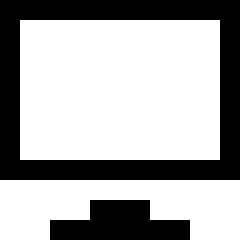
\includegraphics[width=0.5\marginparwidth]{./icons/iconmonstr-computer-6-240.png}}}}
\newenvironment{mentiQuestion}
{\marginpar{%
    \ifodd\value{page}
      \hspace*{-10pt}% odd pages: pull LEFT
    \else
      \hspace*{25pt}% even pages: push RIGHT
    \fi
    \framebox{%
      
\includegraphics[width=0.5\marginparwidth]{icons/iconmonstr-computer-3-240-BLUE.png}%
    }%
  }%
}
{}
%%% Menti Question command
%\usepackage{etoolbox}
%\newcommand{\mentiQuestion}{%
%  \marginpar{%
%    \hfill
%    \framebox{%
%      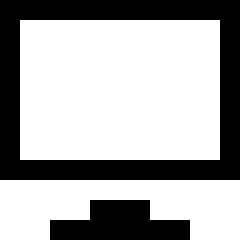
\includegraphics[width=0.5\marginparwidth]{icons/iconmonstr-computer-6-240.png}%
%    }%
%  }%
%}


%%% Hook Pandoc div
%\BeforeBeginEnvironment{startClassBox}{\mentiQuestion}




%%% PreClass box
\definecolor{PreClassColour}{rgb}{0.871, 0.937, 0.745}
\newtcolorbox{preclasscolourbox}{
  colback=PreClassColour,
  colframe=PreClassColour,
  coltext=black,
  boxsep=5pt,
  arc=4pt}
\newenvironment{startClassBox}[1]
  {\small
  \begin{itemize}[leftmargin=.5in]
  \renewcommand{\labelitemi}{
    \raisebox{-.4\height}[0pt][0pt]{
      {\setkeys{Gin}{width=1.5em,keepaspectratio}
        \includegraphics{icons/#1}\qquad}
    }
  }
  \setlength{\fboxsep}{1em}
  \begin{preclasscolourbox}
  \item
  }
  {
  \end{preclasscolourbox}
  \end{itemize}
  } 

%%% PreClass *answers* box
\definecolor{StartClassAnswersColour}{rgb}{0.871, 0.937, 0.745}
\newtcolorbox{startclassanswercolourbox}{
  colback=StartClassAnswersColour,
  colframe=StartClassAnswersColour,
  coltext=black,
  boxsep=5pt,
  arc=4pt}
\newenvironment{startClassAnswersBox}[1]
  {\small
  \begin{itemize}[leftmargin=.5in]
  \renewcommand{\labelitemi}{
    \raisebox{-.4\height}[0pt][0pt]{
      {\setkeys{Gin}{width=1.5em,keepaspectratio}
        \includegraphics{icons/#1}\qquad}
    }
  }
  \setlength{\fboxsep}{1em}
  \begin{startclassanswercolourbox}
  \item
  }
  {
  \end{startclassanswercolourbox}
  \end{itemize}
  } 

  
%%% Drill box
\definecolor{DrillColour}{rgb}{0.871, 0.937, 0.745}
\newtcolorbox{drillcolourbox}{
  colback=DrillColour,
  colframe=DrillColour,
  coltext=black,
  boxsep=5pt,
  arc=4pt}
\newenvironment{drillBox}[1]
  {\small
  \begin{itemize}[leftmargin=.5in]
  \renewcommand{\labelitemi}{
    \raisebox{-.4\height}[0pt][0pt]{
      {\setkeys{Gin}{width=1.5em,keepaspectratio}
        \includegraphics{icons/#1}\qquad}
    }
  }
  \setlength{\fboxsep}{1em}
  \begin{drillcolourbox}
  \item
  }
  {
  \end{drillcolourbox}
  \end{itemize}
  }  
  
  



%%% Optional boxes
\definecolor{OptionalColour}{rgb}{0.871, 0.937, 0.745}
\newtcolorbox{optionalcolourbox}{
  colback=OptionalColour,
  colframe=OptionalColour,
  coltext=black,
  boxsep=5pt,
  arc=4pt}

  
\newenvironment{optionalBox}[1]
  {\small
  \begin{itemize}[leftmargin=.5in]
  \renewcommand{\labelitemi}{
    \raisebox{-.4\height}[0pt][0pt]{
      {\setkeys{Gin}{width=1.5em,keepaspectratio}
        \includegraphics{icons/#1}\qquad}
    }
  }
  \setlength{\fboxsep}{1em}
  \begin{optionalcolourbox}
  \item
  }
  {
  \end{optionalcolourbox}
  \end{itemize}
  }  
  
  
%%% Discuss Box
\definecolor{DiscussColour}{rgb}{0.871, 0.937, 0.745}
\newtcolorbox{discusscolourbox}{
  colback=DiscussColour,
  colframe=DiscussColour,
  coltext=black,
  boxsep=5pt,
  arc=4pt}
\newenvironment{discussBox}[1]
  {
  \begin{itemize}[leftmargin=.5in]
  \renewcommand{\labelitemi}{
    \raisebox{-.4\height}[0pt][0pt]{
      {\setkeys{Gin}{width=1.5em,keepaspectratio}
        \includegraphics{icons/#1}\qquad}
    }
  }
  \setlength{\fboxsep}{1em}
  \begin{discusscolourbox}
  \item
  }
  {
  \end{discusscolourbox}
  \end{itemize}
  }  




% SUPPORT type
% - Common mistakes/warnings
% - Tips
% - Video solutions


%%% Important Box
\definecolor{ImportantColour}{rgb}{0.996, 0.863, 0.761}
\newtcolorbox{importantcolourbox}{
  colback=ImportantColour,
  colframe=ImportantColour,
  coltext=black,
  boxsep=5pt,
  arc=4pt}
\newenvironment{importantBox}[1]
  {\small
  \begin{itemize}[leftmargin=.5in]
  \renewcommand{\labelitemi}{
    \raisebox{-.4\height}[0pt][0pt]{
      {\setkeys{Gin}{width=1.5em,keepaspectratio}
        \includegraphics{icons/#1}\qquad}
    }
  }
  \setlength{\fboxsep}{1em}
  \begin{importantcolourbox}
  \item
  }
  {
  \end{importantcolourbox}
  \end{itemize}
  }  
  
  

%%% Tip boxes
\definecolor{TipColour}{rgb}{0.996, 0.863, 0.761}
\newtcolorbox{tipcolourbox}{
  colback=TipColour,
  colframe=TipColour,
  coltext=black,
  boxsep=5pt,
  arc=4pt}

  
\newenvironment{tipBox}[1]
  {\small
  \begin{itemize}[leftmargin=.5in]
  \renewcommand{\labelitemi}{
    \raisebox{-.4\height}[0pt][0pt]{
      {\setkeys{Gin}{width=1.5em,keepaspectratio}
        \includegraphics{icons/#1}\qquad}
    }
  }
  \setlength{\fboxsep}{1em}
  \begin{tipcolourbox}
  \item
  }
  {
  \end{tipcolourbox}
  \end{itemize}
  }  



  
%%% VideoSolution box
\definecolor{VideoColour}{rgb}{0.996, 0.863, 0.761}
\newtcolorbox{videosolutionscolourbox}{
  colback=VideoColour,
  colframe=VideoColour,
  coltext=black,
  boxsep=5pt,
  arc=4pt}

\newenvironment{videoSolutionBox}[1]
  {\small
  \begin{itemize}[leftmargin=.5in]
  \renewcommand{\labelitemi}{
    \raisebox{-.4\height}[0pt][0pt]{
      {\setkeys{Gin}{width=1.5em,keepaspectratio}
        \includegraphics{icons/#1}\qquad}
    }
  }
  \setlength{\fboxsep}{1em}
  \begin{videosolutionscolourbox}
  \item
  }
  {
  \end{videosolutionscolourbox}
  \end{itemize}
  }  
  
    
  


  

%%% TUTOR-ONLY INFO BOXES
\newenvironment{rmdTutorInfo}
  {\begin{rmdblock}{iconmonstr-school-15-240}}
  {\end{rmdblock}}
  
  

  
%%% END: CALL-OUTS %%%%%%%%%%%%%%%%%%%%%%%%%%%%%%%%%%%%%%%%%%%%%%%%%%%%%%%%%%%%%%%%%%%%%%%%%%%%%%

% Redfine some existing environments
% -QUOTE
\makeatletter
\renewenvironment{quote}
               {\list{}{\vspace{-0.5em}\begin{kframe}\small%
                        \rightmargin   \leftmargin
                        \parsep        \z@ \@plus\p@}%
                \item\relax}
               {\end{kframe}\endlist}
\makeatother


% Change the lemma environment to be shaded
\usepackage{etoolbox}
\usepackage{framed}
\AtBeginEnvironment{lemma}{\begin{shaded}\begin{quote}\vspace{-2em}\setlength{\parskip}{6pt}} % Order must be shaded, then quote
\AtEndEnvironment{lemma}{\end{quote}\end{shaded}}


% ORIGINAL:
%\newenvironment{fold}
%  {\begin{rmdblock}{iconmonstr-idea-12-240}\vspace{-1em}\begin{darkgraytext}\footnotesize \textbf{Answer:}}
%  {\end{darkgraytext}\end{rmdblock}}
\newenvironment{darkgraytext}{\color{textcolor}}{\ignorespacesafterend}
\newenvironment{fold}
  {\vspace{-6pt}\begin{rmdblockNOIMAGE}\begin{darkgraytext}\scriptsize \textbf{Answer:}}
  {\end{darkgraytext}\end{rmdblockNOIMAGE}}
  
% Change the  fold  environment to be disappeared
% Note: In the LaTeX code, it appears like this: \BeginKnitrBlock{fold}
%\usepackage{comment}
%\AtBeginEnvironment{fold}{\begin{comment}}
%\AtEndEnvironment{fold}{\end{comment}}

%\begin{shaded}}
%\AtEndEnvironment{fold}{\end{shaded}}

%%% IF ONLY THIS WORKED:
% \usepackage{comment}
% \includecomment{fold}


%%% Two column chunks: from https://github.com/grantmcdermott/two-col-test/blob/master/preamble.css
\usepackage{multicol}
%% Note: Pandoc (which is doing all of the output conversion behind the scenes) does not parse the content of LaTeX environments. This creates problems when you try to include LaTeX commands with curly brackets directly in your Rmd file. E.g. You can't just use `\begin{multicols}{2}` directly in your Rmd file. Luckily, a straightforward workaround is to simply define some new shortcut commands yourself as per the below.
%% See: https://stackoverflow.com/questions/25849814/rstudio-rmarkdown-both-portrait-and-landscape-layout-in-a-single-pdf/27334272#27334272
\newcommand{\btwocol}{\begin{multicols}{2}}
\newcommand{\etwocol}{\end{multicols}}
            

\usepackage{makeidx}
\makeindex

\usepackage{hyperref}
%\hypersetup{
%    breaklinks = true,     % Allows line breaking of URLs
%    colorlinks = true,     % Colors hyperlinks instead of boxes
%    linkcolor = blue,      % Color for internal links
%    citecolor = blue,      % Color for citations
%    urlcolor = blue        % Color for URLs
%}
\urlstyle{tt}



\makeatother



\frontmatter

%%% Turn off maketitle to get pdf image as title page (https://stackoverflow.com/questions/45963505/coverpage-and-copyright-notice-before-title-in-r-bookdown):
\author{}
\date{\vspace{-2.5em}Last update: \today}
\let\oldmaketitle\maketitle
\AtBeginDocument{\let\maketitle\relax}


% Set headers to just be chapters
\AtBeginDocument{%
  \pagestyle{fancy}
  \fancyhf{}
  
  \renewcommand{\chaptermark}[1]{%
    \markboth{#1}{}%
  }
  
  \renewcommand{\sectionmark}[1]{%
    \markright{#1}%
  }
}




% Taken from: https://bookdown.org/yihui/rmarkdown-cookbook/multi-column.html
\newenvironment{cols}[1][]{}{}

\newenvironment{col}[1]{\begin{minipage}{#1}\ignorespaces}{%
\end{minipage}
\ifhmode\unskip\fi
\aftergroup\useignorespacesandallpars}

\def\useignorespacesandallpars#1\ignorespaces\fi{%
#1\fi\ignorespacesandallpars}

\makeatletter
\def\ignorespacesandallpars{%
  \@ifnextchar\par
    {\expandafter\ignorespacesandallpars\@gobble}%
    {}%
}
\makeatother


\usepackage{bookmark}
\IfFileExists{xurl.sty}{\usepackage{xurl}}{} % add URL line breaks if available
\urlstyle{same}
\hypersetup{
  pdftitle={Science Research Methods: Tutorials},
  pdfauthor={Peter K. Dunn},
  colorlinks=true,
  linkcolor={Maroon},
  filecolor={Maroon},
  citecolor={Blue},
  urlcolor={Blue},
  pdfcreator={LaTeX via pandoc}}

\title{Science Research Methods: Tutorials}
\usepackage{etoolbox}
\makeatletter
\providecommand{\subtitle}[1]{% add subtitle to \maketitle
  \apptocmd{\@title}{\par {\large #1 \par}}{}{}
}
\makeatother
\subtitle{An introduction to quantitative research and statistics}
\author{Peter K. Dunn}
\date{Last updated: June 18, 2026}

\begin{document}
\maketitle



%\killtitle % Removes the title 

%\cleardoublepage\newpage\thispagestyle{empty}\null
%\cleardoublepage\newpage\thispagestyle{empty}\null
%\cleardoublepage\newpage
\thispagestyle{empty}
%\begin{center}
%\includegraphics{images/dedication.pdf}
%\end{center}

\makebox[\textwidth]{
\includegraphics[width=\paperwidth]{images/cover-Tutorial.png}}
%\centerline{\includegraphics[width=\textwidth,height=\textheight]{images/cover.png}}

% Reinstate maketitle (https://stackoverflow.com/questions/45963505/coverpage-and-copyright-notice-before-title-in-r-bookdown):
\let\maketitle\oldmaketitle
\maketitle


\setlength{\abovedisplayskip}{-5pt}
\setlength{\abovedisplayshortskip}{-5pt}

%%% Footer
%\pagestyle{fancy}
%\fancyfoot[L]{\textit{Scientific Research Methods}}


%%% REDEFINE some environments

%%% BASED ONL
%%%   https://stackoverflow.com/questions/58195679/how-can-i-redefine-a-standard-bookdown-theorem-environment-in-latex-pdf (I asked)
%% and adapted using:
%%%   https://stackoverflow.com/questions/1565988/making-a-small-modification-to-a-latex-environment







\let\origexample=\example
\def\example{\begingroup\begin{quote}\setlength{\parskip}{3mm}\vspace{-7mm}\origexample}  
   %% -7mm removes some spacing at the top, which looked odd. Chosen by trial and error
   %% parskip added, otherwise no gap between paras in examples which looked odd.
\let\origendexample=\endexample
\def\endexample{\origendexample\end{quote}\endgroup}


\let\origdefinition=\definition
\def\definition{\begingroup\begin{quote}\vspace{-5mm}\origdefinition}  
   %% -5mm removes some spacing at the top, which looked odd. Chosen by trial and error
\let\origenddefinition=\enddefinition
\def\enddefinition{\origenddefinition\end{quote}\endgroup}


% \let\origlemma=\lemma
% \def\lemma{\begingroup\begin{quote}\vspace{-5mm}\origlemma\normalfont}  
%    %% -5mm removes some spacing at the top, which looked odd. Chosen by trial and error
% \let\origendlemma=\endlemma
% \def\endlemma{\origendlemma\end{quote}\endgroup}
% \renewenvironment{lemma}
%    {\begin{rmdthink}}
%    {\end{rmdthink}}







%%% Greyed background for lemma (now called Think)
% This works, but of course looses all the "lemma" stuff, like numbering and corss-referencing
%\renewenvironment{lemma}
%    {\begin{quote}}
%    {\end{quote}}


% Fix the itemize/enumerate spacing in exercises:
\let\origexercise=\exercise
\def\exercise{\begingroup\setitemize{labelindent=1.5em,labelsep=3mm,leftmargin=*}\setenumerate{labelindent=1.5em,labelsep=3mm,leftmargin=*}\origexercise}  
   %% -5mm removes some spacing at the top, which looked odd. Chosen by trial and error
\let\origendexercise=\endexercise
\def\endexercise{\origendexercise\endgroup}
   %% \setitem  from the  enumitem  package




% Exercise environment does not do dot points correctly: It does this:
%
%   1. This is the
%   way they are done.
%   No hanging pars
%
% So make some adjustments... but it is when itemize is called.


%\renewenvironment{example}[1]%
%  {\begin{quote}\textbf{#1:}}
%  {\end{quote}}

{
\setcounter{tocdepth}{1}
\tableofcontents
}
\chapter*{Preface}\label{preface}


\newcommand{\cms}{\,\text{cm}}
\newcommand{\dLs}{\,\text{dL}}
\newcommand{\xdLs}{\text{dL}}

\newcommand{\fmols}{\,\text{fmol}}
\newcommand{\gs}{\,\text{g}}
\newcommand{\hs}{\,\text{h}}
\newcommand{\xhs}{\text{h}}

\newcommand{\has}{\,\text{ha}}
\newcommand{\xhas}{\text{ha}}

\newcommand{\kgs}{\,\text{kg}}
\newcommand{\kms}{\,\text{km}}
\newcommand{\kWhs}{\,\text{kWh}}
\newcommand{\lbs}{\,\text{lb}}
\newcommand{\Ls}{\,\text{L}}
\newcommand{\xLs}{\text{L}}

\newcommand{\mgs}{\,\text{mg}}
\newcommand{\mls}{\,\text{mL}}
\newcommand{\microgs}{\,\ensuremath{\mu}\text{g}}
\newcommand{\millis}{\,\text{ms}}
\newcommand{\mins}{\,\text{mins}}
\newcommand{\mJs}{\,\text{mJ}}
\newcommand{\MPas}{\,\text{MPa}}
\newcommand{\mmols}{\,\text{mmol}}
\newcommand{\mLs}{\,\text{mL}}
\newcommand{\mms}{\,\text{mm}}
\newcommand{\ms}{\,\text{m}}
\newcommand{\xms}{\text{m}}
\newcommand{\ozs}{\,\text{oz}}
\newcommand{\secs}{\,\text{s}}
\newcommand{\xsecs}{\text{s}}
\newcommand{\ppms}{\,\text{ppm}}
\newcommand{\ys}{\,\text{y}}
\newcommand{\vs}{\,\text{V}}

This book has been prepared for use with the textbook \emph{Scientific Research and Methodology} (available \href{https://peterkdunn.github.io/SRM-Textbook}{free online}, or as a
paper-based textbook, from (for example) \url{https://www.routledge.com}),
to be used in the course \emph{Science Research Methods} at the
University of the Sunshine Coast (UniSC).

This course is an introduction to quantitative research methods in the scientific, engineering and health disciplines.
It introduces the whole research process,
from asking a research question to analysis and reporting of the data.
The focus, however, is on the analysis of data.

\section*{Answers to questions}\label{answers-to-questions}


The answers to most of the tutorial questions are given in App.~\ref{OptionalAnswers}.
In the online version, some answers are implied by working through the online exercises.

\section*{Statistical software}\label{statistical-software}


Most of this book can be read without relying on any specific statistical software.
However, some parts explicitly mention and refer to
jamovi
(\citeproc{ref-Software:jamovi}{The jamovi Project}).
jamovi is \emph{free} to download and use.

\section*{Data sets}\label{data-sets}


Many of the data sets used in this book are available in the \textbf{R} package \texttt{SRMData}, and are listed and available in the companion \href{https://peterkdunn.github.io/SRM-Textbook/AppendixDataSets.html}{textbook}.

\section*{Call-outs used in this book}\label{call-outs-used-in-this-book}


The call-outs used in this book are explained below:

\subsection*{\texorpdfstring{Call-outs to \emph{orient} your study}{Call-outs to orient your study}}\label{call-outs-to-orient-your-study}


\begin{objectivesBox}{iconmonstr-target-4-240.png}
These call-outs introduce the objectives for the sections of the book.

\end{objectivesBox}

\begin{assessmentBox}{iconmonstr-text-check-list-lined-240.png}
These call-out show how the content links to the course assessment.

\end{assessmentBox}

\begin{readBox}{iconmonstr-school-15-240.png}
These call-outs indicate the relevant chapter of the textbook to read.

\end{readBox}

\subsection*{\texorpdfstring{Call-outs to indicate \emph{activities}}{Call-outs to indicate activities}}\label{call-outs-to-indicate-activities}


\begin{drillBox}{iconmonstr-pencil-9-240.png}
These call-outs highlight drill questions, for practising some of the mathematical computations.

\end{drillBox}

\begin{discussBox}{iconmonstr-speech-bubble-26-240.png}
These call-outs are optional discussion topics that your tutor \emph{may} choose to use in tutorials.

\end{discussBox}

\begin{optionalBox}{iconmonstr-help-4-240.png}
These call-outs highlight \textbf{optional} questions, that you might like to complete for personal study.

\end{optionalBox}

\subsection*{\texorpdfstring{Call-outs that give \emph{support}}{Call-outs that give support}}\label{call-outs-that-give-support}


\begin{importantBox}{iconmonstr-warning-8-240.png}
These call-outs highlight common mistakes or warnings, about (for example) a particular concept or about using a formula.

\end{importantBox}

\begin{tipBox}{iconmonstr-info-6-240.png}
These call-outs offer helpful information.

\end{tipBox}

\begin{videoSolutionBox}{iconmonstr-youtube-10-240.png}
This icon flags questions that have \emph{video solutions} in the online book: a narrator works through the question, explaining the solution.

\end{videoSolutionBox}

\section*{How this book was made}\label{how-this-book-was-made}


This book was made using \textbf{R} (\citeproc{ref-Software:Rsoftware}{R Core Team 2018}), and the \textbf{bookdown} package (\citeproc{ref-Software:Rbookdown}{Xie 2016}), based on
Markdown syntax,
using \textbf{knitr} (\citeproc{ref-package:knitr}{Xie 2015}).
Numerous other \textbf{R} packages were used, including:

\begin{itemize}
\tightlist
\item
  \textbf{diagram} (\citeproc{ref-Rpackage:diagram}{Soetaert 2017}) for making some diagrams.
\item
  \textbf{kableExtra} (\citeproc{ref-package:kableExtra}{Zhu 2018}) for nicer tables.
\item
  \textbf{DT} (\citeproc{ref-package:DT}{Xie et al. 2018}) for displaying some data tables in the online version.
\item
  \textbf{viridis} (\citeproc{ref-package:viridis}{Garnier et al. 2024}) for some colour specifications that make colours easier for those with colour-blindness, and for better grey-scale printing.
\item
  \textbf{webexercises} (\citeproc{ref-package:webex}{Barr and DeBruine 2021}) for creating interactive web exercises (i.e., \emph{Quick Revision} questions) in the online version.
\end{itemize}

All of this software is \emph{free} and open source.
Other resources used include:

\begin{itemize}
\tightlist
\item
  The online quizzes are embedded using
  H5P
  iframes.
\item
  Icons are from
  \textbf{iconmonstr},
  and are freely available.
\end{itemize}

\section*{Learning outcomes}\label{learning-outcomes}


\begin{objectivesBox}{iconmonstr-target-4-240.png}

In this book, you will learn to:

\begin{itemize}
\tightlist
\item
  Develop quantitative research questions and testable hypotheses.
\item
  Design quantitative studies to answer simple scientific research questions.
\item
  Select and produce appropriate graphical, numerical and statistical analyses.
\item
  Select, apply and interpret the results of the correct statistical technique to analyse data.
\item
  Comprehend, apply and communicate in the language of research and statistics.
\item
  Demonstrate professional integrity in planning, interpreting and reporting the results of quantitative studies.
\end{itemize}

\end{objectivesBox}

\section*{How to cite this book}\label{how-to-cite-this-book}


Peter K. Dunn (2025).
\emph{Scientific Research and Methodology Tutorial Book: An introduction to quantitative research and statistics in science, engineering and health}.
\url{https://peterkdunn.github.io/SRM-Tutorial-Workbook/index.html}

\mainmatter

\chapter{Teaching Week 1 tutorial}\label{Lecture1}

\begin{objectivesBox}{iconmonstr-target-4-240.png}

You will learn to:

\begin{itemize}
\tightlist
\item
  identify types of research studies.
\item
  ask quantitative research questions.
\item
  use and understand the language used in research.
\end{itemize}

\end{objectivesBox}

\begin{assessmentBox}{iconmonstr-text-check-list-lined-240.png}

The Week~1 content is essential for:

\begin{itemize}
\tightlist
\item
  \textbf{Task~2A}, where you need to \emph{write your own RQ};
\item
  \textbf{Quiz~1}, which includes questions about \emph{writing RQs and RQ components}; and
\item
  the \textbf{Exam}, which will contain questions about \emph{RQs and RQ components}.
\end{itemize}

\end{assessmentBox}

\begin{readBox}{iconmonstr-school-15-240.png}

You will learn and practice the content associated with these chapters of the \href{https://peterkdunn.github.io/SRM-Textbook/}{textbook}:

\begin{itemize}
\tightlist
\item
  \href{https://peterkdunn.github.io/SRM-Textbook/Intro.html}{Chapter 1 (Research: an introduction)}.
\item
  \href{https://peterkdunn.github.io/SRM-Textbook/RQs.html}{Chapter 2 (Research questions)}.
\item
  \href{https://peterkdunn.github.io/SRM-Textbook/FactorsInfluenceY.html}{Chapter 3 (Overview of research design)}.
\item
  \href{https://peterkdunn.github.io/SRM-Textbook/ResearchDesign.html}{Chapter 4 (Types of research studies)}.
\end{itemize}

\end{readBox}

\pagebreak

\section{Quick revision}\label{QuickRevision-Tutorial1}

Consider this RQ (based on Jaworowska et al. (\citeproc{ref-data:jaworowska2012:determination}{2012})):

\begin{quote}
For London take-away restaurants, is the average amount of salt in a Chinese meal the same as in an Indian meal?
\end{quote}

\begin{enumerate}
\def\labelenumi{\arabic{enumi}.}
\item
  What \emph{type} of RQ is this? \tightlist
  Explain your answer, and why the other answers are incorrect.

  \begin{enumerate}
  \def\labelenumii{\alph{enumii}.}
  \tightlist
  \item
    Descriptive.
  \item
    Relational.
  \item
    Repeated-measures.
  \item
    Correlational?
  \end{enumerate}
\item
  What is the \emph{purpose} this RQ? \tightlist

  \begin{enumerate}
  \def\labelenumii{\alph{enumii}.}
  \tightlist
  \item
    Estimation.
  \item
    Decision-making?
  \end{enumerate}
\item
  Is an \emph{intervention} present?
  If so, what is it?
  \answerbox{2}
\item
  What is the \emph{outcome} in this RQ?
  Explain your answer, and why the other answers are incorrect.

  \begin{enumerate}
  \def\labelenumii{\alph{enumii}.}
  \tightlist
  \item
    The amount of salt in each meal.
  \item
    The average amount of salt in Chinese and Indian take-away meals.
  \item
    London take-away restaurants.
  \item
    The average amount of salt.
  \end{enumerate}
\item
  What is the \emph{response variable}?

  \begin{enumerate}
  \def\labelenumii{\alph{enumii}.}
  \tightlist
  \item
    The amount of salt in each meal.
  \item
    The average amount of salt in Chinese and Indian take-away meals.
  \item
    London take-away restaurants.
  \item
    The average amount of salt.
  \end{enumerate}
\item
  What is the \emph{unit of analysis}?
  Explain.

  \begin{enumerate}
  \def\labelenumii{\alph{enumii}.}
  \tightlist
  \item
    We need more information about how the data were collected.
  \item
    Each meal.
  \item
    Each restaurant.
  \end{enumerate}
\item
  What is the \emph{unit of observation}?
  Explain.

  \begin{enumerate}
  \def\labelenumii{\alph{enumii}.}
  \tightlist
  \item
    We need more information about how the data were collected.
  \item
    Each meal.
  \item
    Each restaurant.
  \end{enumerate}
\item
  The article states (p.~518) that ``a takeaway meal was defined as food purchased from out of home food outlets or ordered for home delivery''.
  What \emph{type} of definition is this?

  \begin{enumerate}
  \def\labelenumii{\alph{enumii}.}
  \tightlist
  \item
    Operational.
  \item
    Conceptual
  \end{enumerate}
\end{enumerate}

\section{Class discussion}\label{TW1-Class-Discussion}

\begin{discussBox}{iconmonstr-speech-bubble-26-240.png}
\textbf{Discuss}: In \emph{this} course, in \emph{this} semester, what percentage of students are female?

\end{discussBox}

\section{Research process}\label{ResearchProcess}

Organise the steps of the research process (Fig. \ref{fig:SixStepsToOrder}) into the usual order in which they are used.

\begin{figure}[hbtp]

{\centering \includegraphics[width=0.4\linewidth]{01-TW1-Tutorial_files/figure-latex/SixStepsToOrder-1} 

}

\caption{The six basic steps in research: what is the usual order in which they are  used?}\label{fig:SixStepsToOrder}
\end{figure}

\section{Forming RQs}\label{FormingRQs}

A café owner doesn't believe that his customers can taste the difference between diet and regular colas.
As a result, the owner decides to study this by conducting a study of his customers.

\begin{enumerate}
\def\labelenumi{\arabic{enumi}.}
\item
  Two RQs that the café owner is considering are given below.
  Which do you prefer, and why? \tightlist

  \begin{enumerate}
  \def\labelenumii{\alph{enumii}.}
  \tightlist
  \item
    Among my customers, is the \emph{average} customer-taste rating (on a five-point scale) the same for diet and regular cola drinks?
  \item
    Among my customers, is the \emph{percentage} of customers who prefer diet cola drinks the same as the \emph{percentage} of customers who prefer regular cola drinks?
    \answerbox{2}
  \end{enumerate}
\item
  Develop your own RQ to answer the café owner's question, by carefully and precisely describing P, O, C and I (where relevant).
  \answerbox{3}
\item
  Make notes about \emph{how} the café owner could gather data to answer the RQ.
  \answerbox{3}
\end{enumerate}

\section{Terminology}\label{UnderstandingTerminology1}

Explain the \emph{fundamental differences} between the following pairs of often-confused terms (Table~\ref{tab:SimilarTerms}), highlighting the important differences.

\begin{table}
\centering
\caption{\label{tab:SimilarTerms}Distinguish the similar terms.}
\centering
\fontsize{10}{12}\selectfont
\begin{tabular}[t]{r>{}cl}
\toprule
Hypothesis & \textbf{$\blacktriangleleft$ Pair 1 $\blacktriangleright$} & Research question\\
Relational RQ & \textbf{$\blacktriangleleft$ Pair 2 $\blacktriangleright$} & Repeated-measures RQ\\
\addlinespace
Response variable & \textbf{$\blacktriangleleft$ Pair 3 $\blacktriangleright$} & Explanatory variable\\
Response variable & \textbf{$\blacktriangleleft$ Pair 4 $\blacktriangleright$} & Outcome\\
\addlinespace
Observational study & \textbf{$\blacktriangleleft$ Pair 5 $\blacktriangleright$} & Experimental study\\
Quasi-experiment & \textbf{$\blacktriangleleft$ Pair 6 $\blacktriangleright$} & True experiment\\
\addlinespace
Conceptual definition & \textbf{$\blacktriangleleft$ Pair 7 $\blacktriangleright$} & Operational definition\\
Unit of observation & \textbf{$\blacktriangleleft$ Pair 8 $\blacktriangleright$} & Unit of analysis\\
\bottomrule
\end{tabular}
\end{table}

\section{Terminology}\label{UnderstandingTerminology2}

The use of mobile phones has changed people's behaviour.
Barkley and Lepp (\citeproc{ref-data:Barkley2016:Phones}{2016}) examined how the use of mobile phones impacts walking speed.
Read the following information from the research article (p.~2, 3), and answer the questions that follow, \textbf{explaining} the reason for your choices.
\textbf{Make sure you explain why the other options are incorrect.}

\begin{quote}
The purpose of this study was to compare average walking speed {[}\ldots{]} while individuals were holding a cell phone to their ear (\emph{talking}), actively utilizing the phone with their hands and looking at the screen (\emph{texting}), or not using a cell phone (\emph{no use}).
\end{quote}

\begin{enumerate}
\def\labelenumi{\arabic{enumi}.}
\tightlist
\item
  Which one of these is most likely the \emph{outcome} in the study?
  Explain why the other options are \emph{incorrect}.

  \begin{enumerate}
  \def\labelenumii{\alph{enumii}.}
  \tightlist
  \item
    The way subjects were using their phone.
  \item
    The time taken to walk \(50\)~m.
  \item
    The \textbf{average} time taken to walk \(50\)~m.
  \item
    The difference between the times taken, between those texting and those not texting.
    \answerbox{2}
  \end{enumerate}
\item
  Which one of these is most likely the \emph{comparison} in the study?
  Explain why the other options are \emph{incorrect}.

  \begin{enumerate}
  \def\labelenumii{\alph{enumii}.}
  \tightlist
  \item
    Between the ways that subjects were using their phone (talking; texting; not at all).
  \item
    Between those walking slowly and those walking quickly.
  \item
    Between those walking and those not walking.
  \item
    Between those using and not using a mobile phone.
    \answerbox{2}
  \end{enumerate}
\item
  What is the \emph{explanatory variable}?
  Explain why the other options are \emph{incorrect}.

  \begin{enumerate}
  \def\labelenumii{\alph{enumii}.}
  \tightlist
  \item
    The phone.
  \item
    The way that the phone is being used.
  \item
    The \textbf{average} time to walk \(50\,\text{m}\).
  \item
    The walking speed.
    \answerbox{2}
  \end{enumerate}
\item
  What is the \emph{response variable}?
  Explain why the other options are \emph{incorrect}.

  \begin{enumerate}
  \def\labelenumii{\alph{enumii}.}
  \tightlist
  \item
    The differences between the times taken.
  \item
    The way subjects were using the phone.
  \item
    The \textbf{average} time to walk \(50\,\text{m}\).
  \item
    The time taken to walk \(50\,\text{m}\).
    \answerbox{2}
  \end{enumerate}
\end{enumerate}

\bigskip

\begin{quote}
Naturalistic observations were made, unbeknownst to the subjects {[}\ldots{]} as individuals transversed a 50~m straight walkway on an American college campus {[}\ldots{]}\\
\strut ~

The walkway was straight, had limited ingress and egress, and was simple to navigate.
\end{quote}

\begin{enumerate}
\def\labelenumi{\arabic{enumi}.}
\setcounter{enumi}{4}
\tightlist
\item
  Which one of these is most likely the \emph{population} under study?
  Explain why the other options are \emph{incorrect}.

  \begin{enumerate}
  \def\labelenumii{\alph{enumii}.}
  \tightlist
  \item
    Phones.
  \item
    People.
  \item
    People at an American college.
  \item
    Students at an American college.
    \answerbox{2}
  \end{enumerate}
\item
  Which one of these is most likely the \emph{intervention} in the study?
  Explain why the other options are \emph{incorrect}.

  \begin{enumerate}
  \def\labelenumii{\alph{enumii}.}
  \tightlist
  \item
    The way subjects were using their phones.
  \item
    The timing of the walk.
  \item
    There is no intervention.
  \item
    The phone.
    \answerbox{2}
  \end{enumerate}
\end{enumerate}

\bigskip

\begin{quote}
All observations were made while subjects were walking in one direction (west to east) approaching the overpass where research personnel were positioned.
The starting and end points to the \(50\,\text{m}\) walkway were selected as they had physical landmarks (e.g., a park bench bolted to the walkway) that were easily seen by the observer.\\
\strut ~

Walking speed was recorded, via a stopwatch, as the time (seconds) it took subjects to walk from the start to end points on the \(50\)~m walkway.
~

Walking speed was recorded for every fifth individual, walking independent of others (i.e., alone), to cross the starting point on the \(50\)~m walkway.
\end{quote}

\begin{enumerate}
\def\labelenumi{\arabic{enumi}.}
\setcounter{enumi}{6}
\tightlist
\item
  Which one of these is most likely the \emph{unit of observation} in the study?
  Explain why the other options are \emph{incorrect}.

  \begin{enumerate}
  \def\labelenumii{\alph{enumii}.}
  \tightlist
  \item
    The phone.
  \item
    \emph{Individual} subjects.
  \item
    \emph{Groups} of subjects.
  \item
    Minutes.
    \answerbox{2}
  \end{enumerate}
\item
  Which one of these is most likely the \emph{unit of analysis} in the study?
  Explain why the other options are \emph{incorrect}.

  \begin{enumerate}
  \def\labelenumii{\alph{enumii}.}
  \tightlist
  \item
    The phone.
  \item
    \emph{Individual} subjects.
  \item
    \emph{Groups} of subjects.
  \item
    Minutes.
    \answerbox{2}
  \end{enumerate}
\item
  What is the purpose of recording walking speed for `every fifth individual'?
  \answerbox{2}
\end{enumerate}

\section{Creating research questions and studies}\label{CreateRQs}

Consider the following scenario:

\begin{quote}
While at Café~C one day enjoying a small, organic, almond-milk, half-strength, decaffeinated latte (sometimes called a \emph{Why-Bother}\ldots), Nim sighed, `Exams start next week.
I suppose we'll all start feeling stressed soon.'\\
\strut ~

`Ah,' Jane said, `I had better buy more teabags then.'\\
\strut ~

`Tea bags? Why?' asked Nim, eyebrows raised.\\
\strut ~

`Everyone knows that Earl Grey tea relaxes students\ldots{}' Jane sighed.\\
\strut ~

`How do you know that?' Nim said.\\
\strut ~

`It \emph{does},' snapped Jane.
`Earl Grey relaxes people.'
\end{quote}

Nim considers studying Jane's assertion as the basis for a \textbf{feasible} and \textbf{practical} SCI110 project.

\begin{enumerate}
\def\labelenumi{\arabic{enumi}.}
\tightlist
\item
  Nim needs to determine a \emph{population} to study.
  Which of these would be a useful, feasible and practical population to use?
  Or is there a different population that is `better' to use?
  Explain.

  \begin{enumerate}
  \def\labelenumii{\alph{enumii}.}
  \tightlist
  \item
    All university students.
  \item
    Female university students about to do an exam.
  \item
    UniSC students.
  \item
    Queensland university students.
  \end{enumerate}
\item
  Identify an \emph{outcome} that Nim can measure to answer the research question.
  Justify your answer.
  \answerbox{3}
\item
  Which of these \emph{between-individuals comparisons} do you think Nim should use?
  Why?

  \begin{enumerate}
  \def\labelenumii{\alph{enumii}.}
  \tightlist
  \item
    Between drinking Earl Grey tea and coffee.
  \item
    Between drinking Earl Grey tea and black (ordinary) tea.
  \item
    Between drinking Earl Grey tea and water.
  \item
    Between exam time and other times of the semester.
  \item
    Between students and non-students.
  \end{enumerate}
\item
  Explain why `Between before and after drinking Earl Grey tea' is a \emph{within-individuals} comparison.
  \answerbox{3}
\item
  Construct a well-worded \emph{relational} research question \emph{with an intervention} based on your P, O and~C.
  \answerbox{3}
\item
  \emph{Briefly} describe an \emph{experimental} study for answering this proposed research question.
  \answerbox{3}
\item
  Construct a well-worded \emph{relational} research question \emph{without an intervention} based on your P, O and~C.
  \answerbox{3}
\item
  \emph{Briefly} describe an \emph{observational} study for answering this proposed research question.
  \answerbox{3}
\item
  List any necessary word or terms that need operational or conceptual definitions.
  (You do not need to \emph{give} the definitions.)
  \answerbox{2}
\item
  Using this research question, identify the \textbf{response} and \textbf{explanatory} variables, and hence the data that \emph{needs} to be collected to answer the question.
  \answerbox{2}
\end{enumerate}

\section{Identifying units of analysis and units of observation}\label{Units}

Bamboo is a fast-growing, strong grass often used for environmentally-friendly building practices.
A small research study explored the hardness of bamboo when used as flooring material.

The \emph{Janka hardness}\footnote{The force required to embed an \(11.28\,\text{mm}\) steel ball into wood to a depth of half the diameter of the ball.} of bamboo flooring provided by Bamboo Flooring Australia Pty Ltd was measured by the Queensland Department of Primary Industries (\citeproc{ref-data:Gerber:BambooFlooring}{Gerber 2004}).
Five floorboards had two hardness measurements taken on \emph{each} board (units probably kilonewtons; Table~\ref{tab:JankaBoards}).

\begin{table}
\centering
\caption{\label{tab:JankaBoards}Two Janka hardness measurements from five different bamboo boards..}
\centering
\fontsize{10}{12}\selectfont
\begin{tabular}[t]{ccccc}
\toprule
\textbf{Board 1} & \textbf{Board 2} & \textbf{Board 3} & \textbf{Board 4} & \textbf{Board 5}\\
\midrule
$\phantom{0}10.5$ & $\phantom{0}8.0$ & $\phantom{0}11.5$ & $\phantom{0}10.3$ & $\phantom{0}10.2$\\
$\phantom{0}\phantom{0}7.5$ & $\phantom{0}8.0$ & $\phantom{0}11.2$ & $\phantom{0}\phantom{0}9.9$ & $\phantom{0}\phantom{0}9.3$\\
\bottomrule
\end{tabular}
\end{table}

\begin{enumerate}
\def\labelenumi{\arabic{enumi}.}
\tightlist
\item
  What is the unit of analysis: the test, the board, the Janka hardness, each measurement, kilonewtons, or something else?
  Explain your answer.
  \answerbox{2}
\item
  \emph{How many} units of analysis are there?
  \answerbox{1}
\item
  \emph{How many} units of observation are there?
  \answerbox{1}
\item
  Suppose the measurements were all taken from \(10\)~\emph{different} places on the \emph{same} board (rather than from five different boards).
  How many units of analysis are there now?
  Explain your answer.
  \answerbox{2}
\item
  Comment on the amount of variation \emph{between} the boards compared to the amount of variation \emph{within} boards.
  \answerbox{2}
\end{enumerate}

\section{\texorpdfstring{\textbf{Optional questions}}{Optional questions}}\label{OptionalTW1}

\begin{optionalBox}{iconmonstr-help-4-240.png}
These questions are \textbf{optional}; e.g., if you need more practice, or you are studying for the exam.
(Answers appear in Sect.~\ref{Lecture1Answers}.)

\end{optionalBox}

\subsection{\texorpdfstring{\textbf{(Optional)} Identifying different types of studies}{(Optional) Identifying different types of studies}}\label{TypesOfStudies}

\begin{enumerate}
\def\labelenumi{\arabic{enumi}.}
\item
  A lecturer wishes to compare the average blood alcohol concentrations (BAC) of students in two of her classes.
  She measures the BAC of students in two of her Monday morning classes.

  What \emph{type} of study is this: observational, true experimental, quasi-experimental?
  Explain.
\item
  A lecturer wishes to compare the average BAC of students in two of her classes,
  to determine if knowing in advance leads to different average BAC.

  She informs one class on a Friday that she will be measuring BAC in students on a Monday morning,
  but does not tell another of her Friday classes.

  What type of study is this: observational, true experimental, quasi-experimental?
  Explain.
\end{enumerate}

\pagebreak

\subsection{\texorpdfstring{\textbf{(Optional)} Terminology}{(Optional) Terminology}}\label{TerminologyLect1}

Complete the crossword
in Fig. \ref{fig:Crossword-Week1-Terminology}
to help you understand some of the words used in the content.

\begin{figure}[hbtp]

{\centering 
\includegraphics[width=0.7\linewidth]{images/Crossword-Week1} 

}

\caption{A crossword to complete.}\label{fig:Crossword-Week1-Terminology}
\end{figure}

\begin{multicols}{2}\small

\textbf{Across}
\begin{enumerate}\tightlist
  \item[\textbf{2.}]
  The second step in the research process (6)  
  \item[\textbf{3.}]
  The type of research where data are summarised using numerical methods (and is studied in SCI110) (12)
  \item[\textbf{5.}]
  What is Australia's national gemstone? (4)  
  \item[\textbf{6.}]
  Research is used to provide \verb|________|-based answers to RQs (8)  
  \item[\textbf{7.}] 
  The first step in the research process is to \verb|___| the research question (3)  
  \item[\textbf{9.}]
  RQs in which groups are compared numerically are called \verb|__________| (10)  
  \item[\textbf{12.}]
  RQs may be decision making-type RQs or \verb|__________|-type RQs (10)  
  \item[\textbf{15.}]
  What we do with the data to find an answer to the RQ (7)  
  \item[\textbf{16.}] 
  What is the name of Australia's wild dog? (5)
  \item[\textbf{17.}] 
  What is the abbreviation for Australia's island state? (3)
\end{enumerate}

\columnbreak

\textbf{Down}
\begin{enumerate}\tightlist
  \item[\textbf{1.}]
  Independent collections of units of observations are called units of \verb|________| (8)
  \item[\textbf{2.}]
  `Conceptual' and `Operational' are different types of \verb|___________| (11)  
  \item[\textbf{3.}]
  The type of research where data are \emph{not} summarised using numerical methods (11)  
  \item[\textbf{4.}] 
  What is a baby koala called? (4)
  \item[\textbf{6.}]
  What bird is on the Australian coat of arms? (3)
  \item[\textbf{8.}]
  The collected information to answer the RQ is called \verb|____| (4)  
  \item[\textbf{10.}]
  A confounding variable, that is not measured or recorded, is a \verb|_______| variable (7)
  \item[\textbf{11.}]
  After designing a study, the next step is to \verb|_______| the data (7)  
  \item[\textbf{13.}]
  The acronym to remember the four components of a RQ (4)
  \item[\textbf{14.}]
  The sample size is the number of \verb|_____| of analysis (5)
\end{enumerate}
\end{multicols}

\chapter{Teaching Week 2 tutorial}\label{Lecture2}

\begin{objectivesBox}{iconmonstr-target-4-240.png}

You will learn to:

\begin{itemize}
\tightlist
\item
  design quantitative research studies to answer RQs.
\item
  use and understand the language used in research.
\end{itemize}

\end{objectivesBox}

\begin{assessmentBox}{iconmonstr-text-check-list-lined-240.png}

The Week~2 content is essential for:

\begin{itemize}
\tightlist
\item
  \textbf{Task~2A}, which is largely about the \emph{research design} for answering your own RQ;
\item
  \textbf{Quiz~1}, which includes questions about \emph{research design}; and
\item
  the \textbf{Exam}, which will contain questions about \emph{research design}.
\end{itemize}

\end{assessmentBox}

\begin{readBox}{iconmonstr-school-15-240.png}

You will learn and practice the content associated with these chapters of the \href{https://peterkdunn.github.io/SRM-Textbook/}{textbook}:

\begin{itemize}
\tightlist
\item
  \href{https://peterkdunn.github.io/SRM-Textbook/Ethics.html}{Chapter 5 (Ethics in research)}.
\item
  \href{https://peterkdunn.github.io/SRM-Textbook/Sampling.html}{Chapter 6 (External validity: sampling)}.
\item
  \href{https://peterkdunn.github.io/SRM-Textbook/DesignInternal.html}{Chapter 7 (Internal validity)}.
\item
  \href{https://peterkdunn.github.io/SRM-Textbook/Interpretation.html}{Chapter 8 (Research design limitations)}.
\end{itemize}

\end{readBox}

\begin{tipBox}{iconmonstr-info-6-240.png}
You should bring your calculator to tutorials from \textbf{next week onwards}.

\end{tipBox}

\pagebreak

\section{Quick revision}\label{QuickRevision-Tutorial2}

Consider this RQ (\citeproc{ref-walters2018factors}{Walters et al. 2018}):

\begin{quote}
What factors are preventing the adoption of household solar technologies in Santiago {[}Chile{]}?'
\end{quote}

\begin{enumerate}
\def\labelenumi{\arabic{enumi}.}
\tightlist
\item
  For this RQ, what is the \emph{Population}? \tightlist

  \begin{enumerate}
  \def\labelenumii{\alph{enumii}.}
  \tightlist
  \item
    Solar technologies.
  \item
    Household in the world.
  \item
    Household in Chile.
  \item
    Household in Santiago.
  \end{enumerate}
\item
  The study will be \emph{externally valid} if:

  \begin{enumerate}
  \def\labelenumii{\alph{enumii}.}
  \tightlist
  \item
    The sample is representative of all households in Santiago.
  \item
    The sample is representative of all households in Chile.
  \item
    The sample is representative of all solar technologies.
  \item
    The sample is representative of all households in the world.
  \end{enumerate}
\item
  Suppose the researchers mailed surveys to all households in Santiago, and people returned the survey if they wished to.
  What is the \emph{best} description of this sampling method?

  \begin{enumerate}
  \def\labelenumii{\alph{enumii}.}
  \tightlist
  \item
    Systematic sampling.
  \item
    Convenience sampling.
  \item
    Self-selecting sampling.
  \item
    None of the other answers are correct.
  \end{enumerate}
\item
  Suppose the researchers randomly selected five suburbs in Santiago; then ten streets within each of these suburbs; then ten households within each of these streets.
  What is the \emph{best} description of this sampling method?

  \begin{enumerate}
  \def\labelenumii{\alph{enumii}.}
  \tightlist
  \item
    Stratified sampling.
  \item
    Systematic sampling.
  \item
    Multi-stage sampling.
  \item
    None of the other answers are correct.
  \end{enumerate}
\item
  Suppose the researchers stood outside a busy supermarket, and surveyed every ninth person who entered.
  What is the \emph{best} description of this sampling method?

  \begin{enumerate}
  \def\labelenumii{\alph{enumii}.}
  \tightlist
  \item
    Stratified sampling.
  \item
    Systematic sampling.
  \item
    Multi-stage sampling.
  \item
    None of the other answers are correct.
  \end{enumerate}
\end{enumerate}

\section{Study design}\label{StudyDesign}

A student group was studying this RQ (which is \textbf{not} appropriate for the SCI110 Project; Task 2):

\begin{quote}
Among Australians, is the average serum cholesterol concentration different for smokers and non-smokers?
\end{quote}

Explain \emph{why}, according to the \emph{Guidelines}, this RQ is \emph{not} appropriate for Task~2.
\answerbox{2}

The students gave the following information about their study.
Explain \textbf{why} each of these statements is \textbf{incorrect}.

\begin{enumerate}
\def\labelenumi{\arabic{enumi}.}
\tightlist
\item
  ``The design is observational, as we cannot manipulate each person's serum cholesterol.''
  \answerbox{2}
\item
  ``The Outcome is \emph{the average serum cholesterol concentration for smokers and non-smokers}.''
  \answerbox{2}
\item
  ``The study is \emph{not} externally valid, as the results may not apply to all people in the world.''
  \answerbox{2}
\item
  ``The response variable is \emph{serum cholesterol}.''
  \answerbox{2}
\item
  ``In this experiment, the population is \emph{Australians}.''
  \answerbox{2}
\item
  ``The data file will have two columns: one with serum cholesterol concentration for smokers, and one with serum cholesterol concentration for non-smokers.''
  \answerbox{2}
\item
  ``\emph{Whether or not the person owns a cat} is likely to be a confounding variable.''
  \answerbox{2}
\item
  ``The \emph{observer effect} is not relevant, as the participants will know they are involved in a study.''
  \answerbox{2}
\end{enumerate}

\section{Language}\label{LanguageReport}

Patients who have suffered a stroke often have restricted limb movement, and rehabilitation therapies are studying robotics to assist these patients.
Read the description (line breaks added for clarity) of one such study (\citeproc{ref-data:Lo2010:RobotAssistance}{Lo et al. 2010}), then complete the crossword
in Fig. \ref{fig:Crossword-Week2-Terminology}
regarding this information.

\begin{quote}
In this multicenter, randomized, controlled trial involving \(127\) patients with moderate-to-severe upper-limb impairment \(6\)~months or more after a stroke, we randomly assigned \(49\)~patients to receive intensive robot-assisted therapy, \(50\) to receive intensive comparison therapy, and \(28\)~to receive usual care.\\
\strut ~

Therapy consisted of \(36\) \(1\)-hour sessions over {[}\ldots{]} \(12\)~weeks.
The primary outcome was a change in motor function {[}\ldots{]} at \(12\)~weeks\ldots{}\\
\strut ~

We recruited veterans from four participating VA medical centers who were \(18\)~years of age or older and had long-term, moderate-to-severe motor impairment of an upper limb from a stroke that had occurred at least \(6\) months before enrollment.\\
\strut ~

Such impairment was defined as a score of~\(7\) to~\(38\) on the Fugl-Meyer Assessment of Sensorimotor Recovery after Stroke, a scale with scores for upper-limb impairment ranging from~\(0\) (no function) to~\(66\) (normal function).
All patients provided written informed consent.
Patients were randomly assigned to receive robot-assisted therapy, intensive comparison therapy, or usual care\ldots{}\\
\strut ~

Trained evaluators who were unaware of study-group assignments assessed patients~\(6\), \(12\), \(24\), and \(36\)~weeks after randomization.
The primary outcome was a change in the Fugl-Meyer score at \(12\)~weeks, as compared with the baseline value\ldots{}

--- Lo et al. (\citeproc{ref-data:Lo2010:RobotAssistance}{2010})
\end{quote}

\pagebreak

\begin{figure}[hbtp]

{\centering 
\includegraphics[width=0.85\linewidth]{images/Crossword-Week2} 

}

\caption{A crossword to complete.}\label{fig:Crossword-Week2-Terminology}
\end{figure}

\begin{multicols}{2}\small
\textbf{Across}
\begin{enumerate}\tightlist
  \item[\textbf{2.}]
  The type of tree that koalas feed on (3)  
  \item[\textbf{3.}]
  The evaluators were unaware of the group the patient was in; they were \verb|_____| to the treatment (5)
  \item[\textbf{5.}]
  Informed consent ensures the study is \verb|_______| (7)
  \item[\textbf{7.}]
  Canberra is in what state or territory? (3)
  \item[\textbf{8.}]
  When individuals change their behaviour if they think they are being observed: the \verb|_________| effect (9)
  \item[\textbf{11.}]
  The type of therapy is called the \verb|_________| (9)
  \item[\textbf{12.}]
  The research question is of this type (10)
  \item[\textbf{13.}]
  Riddle: Feed me, I live; water me, I die (4)
  \item[\textbf{14.}]
  Patients were assigned \verb|________| to the type of therapy received (8)  
\end{enumerate}

\columnbreak

\textbf{Down}
\begin{enumerate}\tightlist
  \item[\textbf{1.}]
  The size of the \verb|______| is $127$ (6)
  \item[\textbf{3.}]
  A lovely place to relax, with sand and surf (5)
  \item[\textbf{4.}]
  What is the famous rock in central Australia? (5)
  \item[\textbf{5.}]
  This type of study is called a \verb|____________| study (12)  
  \item[\textbf{6.}] 
  Ask if you need \verb|____| (e.g., in tutorial, or on the Canvas \textit{Discussions}) (4)  
  \item[\textbf{9.}]
  The treatment of `usual care' would be considered to be the \verb|_______| group (7)
  \item[\textbf{10.}]
  The number of groups being compared (5)  
  \item[\textbf{15.}]
  What is Australia's largest cricket oval? (3)
\end{enumerate}
\end{multicols}

\section{Assessing reports}\label{AssessReport}

A report in \emph{The Sydney Morning Herald} (\citeproc{ref-data:Berry:AgedCheese}{Berry 2016}) was entitled `Aged cheese could help you age well'.
The research was based partly on a study of mice, and partly on a study of people.
Based on this headline, answer the following questions.

\begin{enumerate}
\def\labelenumi{\arabic{enumi}.}
\tightlist
\item
  What are reasonable suggestions for the outcome and response variable, given this headline? \tightlist
  \answerbox{2}
\item
  What are reasonable suggestions for the comparison and explanatory variable, given this headline?
  \answerbox{2}
\item
  Would you expect the study to be observational or experimental?
  Explain.
  \answerbox{2}
\end{enumerate}

Below is an extract from the newspaper article about the mice study that formed part of the research.

\begin{quote}
Cheese is not only delicious and nutritious {[}\ldots{]} it can also slow down the ageing process, according to a new study {[}\ldots{]}
In the study published in the journal \emph{Nature Medicine}, European researchers analysed the effect of a compound found in aged cheese (as well as legumes and whole grains) called spermidine {[}\ldots{]}
the team supplemented the drinking water of mice with spermidine.
Control mice drank normal water.
\end{quote}

The researchers then found that the addition of spermidine `\,``significantly extended'' the {[}average{]} lifespan of the mice\ldots{}'.
Based on this information, answer the following questions.

\begin{enumerate}
\def\labelenumi{\arabic{enumi}.}
\setcounter{enumi}{3}
\tightlist
\item
  What are reasonable suggestions for the outcome and response variable for the mice study? \tightlist
  \answerbox{2}
\item
  What are reasonable suggestions for the comparison and explanatory variable?
  \answerbox{2}
\item
  Is the study observational or experimental?
  Explain.
  \answerbox{2}
\item
  Does the newspaper headline appear reasonable?
  \answerbox{1}
\item
  Why do the researchers give some mice plain drinking water?
  \answerbox{2}
\end{enumerate}

Below is an extract from the newspaper article for the human study that formed part of the research.

\begin{quote}
\ldots{} the researchers surveyed \(800\) Italians about their diet and found that those who reported a higher intake of spermidine had lower blood pressure\ldots{}
\end{quote}

Based on this information, answer the following questions.

\begin{enumerate}
\def\labelenumi{\arabic{enumi}.}
\setcounter{enumi}{8}
\tightlist
\item
  What are reasonable suggestions for the outcome and response variable for the human study? \tightlist
  \answerbox{2}
\item
  What \emph{type} of RQ is suggested: relational, correlational or repeated-measures?
  \answerbox{1}
\item
  Is the study observational or experimental?
  Explain.
  \answerbox{2}
\end{enumerate}

\pagebreak

\begin{enumerate}
\def\labelenumi{\arabic{enumi}.}
\setcounter{enumi}{11}
\item
  Are the following variables likely to be extraneous variables, control variables, confounding variables, or none of these?
  \textbf{Explain.}

  \begin{enumerate}
  \def\labelenumii{\alph{enumii}.}
  \tightlist
  \item
    The sex of the person.
  \item
    The number of siblings.
  \item
    The distance to the nearest hospital.
  \item
    The amount of exercise per week by the person.
  \item
    Whether their father had heart problems.
    \answerbox{4}
  \end{enumerate}
\end{enumerate}

The newspaper article is based on a research paper (\citeproc{ref-eisenberg2016cardioprotection}{{Eisenberg et al.} 2016}), in which the diets of more than \(800\) Italians were recorded in~1995, 2000 and~2005 for the people-study.
From 1995 to~2010, the researchers recorded heart-related events for each subject: incidents of high blood pressure, heart failure, stroke and premature death from heart disease.

Those with the highest spermidine intakes had a \(40\)\% lower risk of heart failure (both fatal and non-fatal) compared to those with the lowest spermidine intakes.
Those with the highest spermidine intakes also had a significantly lower risk of \emph{any} heart disease, compared to those with the lowest spermidine intakes.

\begin{enumerate}
\def\labelenumi{\arabic{enumi}.}
\setcounter{enumi}{12}
\tightlist
\item
  Does the newspaper headline appear consistent with the research article?
  \answerbox{1}
\end{enumerate}

The study reports that the biggest contributors to spermidine intakes were:

\begin{itemize}
\tightlist
\item
  wholemeal foods (accounting for \(13.4\)\% of intake);
\item
  apples and pears (\(13.3\)\%),
\item
  salad (\(9.8\)\%),
\item
  vegetable sprouts (\(7.3\)\%), and
\item
  potatoes (\(6.4\)\%).
\item
  aged cheese (\(2.9\)\%).
\end{itemize}

\begin{enumerate}
\def\labelenumi{\arabic{enumi}.}
\setcounter{enumi}{13}
\tightlist
\item
  Based on this information, do you agree with, or not agree with, the newspaper article headline?
  Explain.
  \answerbox{2}
\item
  Is the cause-and-effect relationship, as implied in the article headline, reasonable?
  Explain.
  \answerbox{2}
\item
  What did you learn from this study?
  \answerbox{1}
\end{enumerate}

\nopagebreak

\section{Class discussion: planning a research study}\label{PlanStudy2}

\begin{tipBox}{iconmonstr-info-6-240.png}
This activity is very important for helping with your Project.

\end{tipBox}

\begin{discussBox}{iconmonstr-speech-bubble-26-240.png}
Your tutor will have
information.

\end{discussBox}

\section{Study design features}\label{StudyFeatures}

A study (\citeproc{ref-data:Truswell1992:crisps}{Truswell et al. 1992}) compared the health benefits of crisps (`potato chips') when fried in canola oil or palmolein.
The article states (line breaks added):

\begin{quote}
Recently canola oil crisps have appeared in the market with the implication that their lower proportion of saturated fatty acids would have beneficial effects on plasma cholesterol.\\
\strut ~

We decided to examine this experimentally\ldots{} a major manufacturer agreed to fry batches of potato crisps in canola oil or the conventional palmolein for a human trial.
This provided an opportunity for us to run a double blind crossover trial.

--- Truswell et al. (\citeproc{ref-data:Truswell1992:crisps}{1992})
\end{quote}

Part of the protocol for the study is given below:

\begin{quote}
Subjects were asked to eat about a third of the day's crisps at the beginning of each meal and then, in the rest of their diets, to eat foods that were low to moderate in fat from a list of such foods\ldots{}\\
\strut ~

The crisps were supplied in plain bags, unmarked except for two code characters: `T4' or `B9' in 1990 and `D5' or `GS' in 1991.
Until the end of the experiment, the type of oil was known only by the food scientist who prepared the crisps.\\
\strut ~

In 1990, \(21\) subjects (\(12\) men, \(9\) women) completed the \(5\)~week experiment.
They were randomly allocated to take palmolein (`B9') or canola (`T4') crisps for the first \(3\) weeks, then (without a washout period) changed over to the other type, canola or palmolein for another \(2\) weeks.
Thus half the subjects ate (new) canola crisps for \(3\) weeks and the (usual) palmolein crisps for the next \(2\) weeks.\\
\strut ~

The other half of the subjects ate palmolein crisps for \(3\) weeks and canola crisps for the next \(2\) weeks.
The first week of the \(3\) weeks served as an adjustment period.
Fasting venous bloods were taken once at the start (usual diet), then for the last \(3\) mornings of both the first and second experimental periods.

--- Truswell et al. (\citeproc{ref-data:Truswell1992:crisps}{1992})
\end{quote}

\begin{enumerate}
\def\labelenumi{\arabic{enumi}.}
\tightlist
\item
  Explain how random \emph{allocation} is used (and why), if at all.
  \answerbox{2}
\item
  Explain how the impact of the Hawthorne effect has been minimised.
  \answerbox{2}
\item
  Explain how the impact of the observer effect has been minimised.
  \answerbox{2}
\item
  Would the carry-over effect play a role? Explain.
  \answerbox{2}
\item
  Describe the blinding that is used.
  \answerbox{2}
\end{enumerate}

\chapter{Teaching Week 3 tutorial}\label{Lecture3}

\begin{objectivesBox}{iconmonstr-target-4-240.png}

You will learn to:

\begin{itemize}
\tightlist
\item
  collect data.
\item
  classify data.
\item
  produce and understand graphical summaries for quantitative data.
\item
  produce and understand numerical summaries for quantitative data.
\end{itemize}

\end{objectivesBox}

\begin{assessmentBox}{iconmonstr-text-check-list-lined-240.png}

The Week~3 content is essential for:

\begin{itemize}
\tightlist
\item
  \textbf{Task~2A}, which requires you to \emph{classify variables and suggest appropriate numerical and appropriate graphical summaries};
\item
  \textbf{Task~2B}, which requires you to \emph{collect your own data, classify variables, produce appropriate numerical summaries, and produce appropriate graphs};
\item
  \textbf{Quiz~2}, which includes questions about \emph{classifying variables, numerical summaries and graphs}; and
\item
  the \textbf{Exam}, which will contain questions about \emph{classifying variables, numerical summaries and graphs}.
\end{itemize}

\end{assessmentBox}

\begin{readBox}{iconmonstr-school-15-240.png}

You will learn and practice the content associated with these chapters of the \href{https://peterkdunn.github.io/SRM-Textbook/}{textbook}:

\begin{itemize}
\tightlist
\item
  \href{https://peterkdunn.github.io/SRM-Textbook/CollectingDataProcedures.html}{Chapter 9 (Collecting data)}.
\item
  \href{https://peterkdunn.github.io/SRM-Textbook/DescribingVars.html}{Chapter 10 (Classifying data and variables)}.
\item
  \href{https://peterkdunn.github.io/SRM-Textbook/SummariseQuantData.html}{Chapter 11 (Summarising quantitative data)}.
\end{itemize}

\end{readBox}

\begin{tipBox}{iconmonstr-info-6-240.png}
You should bring your calculator to tutorials \textbf{from this week onwards}.

\end{tipBox}

\begin{tipBox}{iconmonstr-info-6-240.png}
You can search on YouTube for tutorials on using your calculator's \textbf{Statistics Mode}.
For example:

\texttt{"statistics"\ "mean"\ "standard\ deviation"\ Casio\ fx82}

\end{tipBox}

\pagebreak

\section{Quick revision}\label{QuickRevision-Tutorial3}

In a study of obstructive sleep apnoea (OSA) in adults with Down Syndrome (\citeproc{ref-carvalho2020stop}{{de Carvalho et al.} 2020}), \(n = 60\) adults underwent a sleep study.
Part of the data are shown in Table~\ref{tab:OSAKable}.
(REI is the Respiratory Event Index; REI under~\(5\) refers to no sleep apnoea; REI of \(30\)~or over refers to severe sleep apnoea.)

\begin{enumerate}
\def\labelenumi{\arabic{enumi}.}
\tightlist
\item
  How would you \emph{classify} the variable \texttt{Age}? \tightlist

  \begin{enumerate}
  \def\labelenumii{\alph{enumii}.}
  \tightlist
  \item
    Qualitative nominal
  \item
    Qualitative ordinal
  \item
    Quantitative discrete
  \item
    Quantitative continuous
  \end{enumerate}
\item
  How would you \emph{classify} the variable \texttt{Gender}? \tightlist

  \begin{enumerate}
  \def\labelenumii{\alph{enumii}.}
  \tightlist
  \item
    Qualitative nominal
  \item
    Qualitative ordinal
  \item
    Quantitative discrete
  \item
    Quantitative continuous
  \end{enumerate}
\item
  How would you \emph{classify} the variable \texttt{BMI}? \tightlist

  \begin{enumerate}
  \def\labelenumii{\alph{enumii}.}
  \tightlist
  \item
    Qualitative nominal
  \item
    Qualitative ordinal
  \item
    Quantitative discrete
  \item
    Quantitative continuous
  \end{enumerate}
\item
  How would you \emph{classify} the variable \texttt{REI}? \tightlist

  \begin{enumerate}
  \def\labelenumii{\alph{enumii}.}
  \tightlist
  \item
    Qualitative nominal
  \item
    Qualitative ordinal
  \item
    Quantitative discrete
  \item
    Quantitative continuous
  \end{enumerate}
\end{enumerate}

\begin{table}
\centering
\caption{\label{tab:OSAKable}Part of the obstructive sleep apnoea data set ($n = 60$).}
\centering
\fontsize{10}{12}\selectfont
\begin{tabular}[t]{ccccc}
\toprule
\textbf{Age} & \textbf{Gender} & \textbf{BMI} & \textbf{Neck circumference (cm)} & \textbf{REI}\\
\midrule
21 & Male & 20.3 & 37 & 46\\
24 & Male & 24.1 & 40.5 & 19.3\\
26 & Male & 25.2 & 38 & 12.4\\
39 & Female & 40.8 & 41 & 58.6\\
21 & Female & 35 & 37 & 12.7\\
\addlinespace
29 & Male & 29.2 & 41 & 38.8\\
20 & Male & 25.8 & 42 & 24.4\\
21 & Male & 20.9 & 37 & 7\\
19 & Female & 20.5 & 32 & 37.6\\
27 & Male & 22.4 & 39 & 21.7\\
\addlinespace
$\vdots$ & $\vdots$ & $\vdots$ & $\vdots$ & $\vdots$\\
\bottomrule
\end{tabular}
\end{table}

\section{Class discussion}\label{TW3-Class-Discussion}

\begin{discussBox}{iconmonstr-speech-bubble-26-240.png}
\textbf{Discuss}: Two datasets can have the same numerical summaries but tell very different stories.

\end{discussBox}

\section{\texorpdfstring{Using the calculator \emph{Statistics Mode} for a small data set}{Using the calculator Statistics Mode for a small data set}}\label{StatsMode}

Table~\ref{tab:PolyTable} shows the polythene usage, in tonnes, by eight UK cosmetic companies (\citeproc{ref-gilchrist2000regression}{Gilchrist 2000}).

\begin{enumerate}
\def\labelenumi{\arabic{enumi}.}
\tightlist
\item
  Using your calculator's \emph{Statistics Mode}, find the \textbf{mean} and \textbf{standard deviation} of these numbers.
  \answerbox{2}
\item
  Without using a calculator, find the \textbf{median} of the data.
  \answerbox{2}
\item
  Without using a calculator, find the \textbf{IQR} of the data.
  \answerbox{2}
\end{enumerate}

\begin{table}
\centering
\caption{\label{tab:PolyTable}The amount of polythene (in tonnes) used by a sample of eight UK cosmetic companies.}
\centering
\fontsize{10}{12}\selectfont
\begin{tabular}[t]{llllllll}
\toprule
$\phantom{0}\phantom{0}\phantom{0}8.001$ & $\phantom{0}\phantom{0}29.400$ & $\phantom{0}266.532$ & $4298.700$ & $\phantom{0}\phantom{0}94.500$ & $2547.300$ & $\phantom{0}676.200$ & $\phantom{0}\phantom{0}\phantom{0}0.000$\\
\bottomrule
\end{tabular}
\end{table}

\begin{importantBox}{iconmonstr-warning-8-240.png}
Most calculators have \textbf{two buttons} that compute the standard deviation when in \emph{Statistics Mode}: one computes the standard deviation if the data are a sample, and one if the data are a population.
In practice, data are almost \emph{never} a population.\\
\strut ~

If you are using your calculator correctly, you should get (before rounding) \(\bar{x} = 990.0791\) and \(s = 1588.514579\).
If you get \(s = 1485.919327\) for the \emph{standard deviation}, you are using your calculator incorrectly, so please \textbf{ask for help}: you are probably pressing the incorrect button to get the standard deviation.

\end{importantBox}

\section{Understanding centre and variation}\label{UnderstandingVariation}

A tutor has recorded the marks (as a percentage) for all students in her four classes for an assignment.
All classes have \(30\)~students.
The corresponding histograms are shown in Fig.~\ref{fig:VariationHistograms}.

\begin{enumerate}
\def\labelenumi{\arabic{enumi}.}
\tightlist
\item
  In which class would the median be the \emph{largest}?
  Why?
  \answerbox{2}
\item
  In which class would the median be the \emph{smallest}?
  Why?
  \answerbox{2}
\item
  In which class would the standard deviation be the \emph{largest}?
  Why?
  \answerbox{2}
\item
  In which class would the standard deviation be the \emph{smallest}?
  Why?
  \answerbox{2}
\end{enumerate}

\begin{figure}[hbtp]

{\centering 
\includegraphics[width=0.9\linewidth]{03-TW3-Tutorial_files/figure-latex/VariationHistograms-1} 

}

\caption{Histogram of marks for four classes.}\label{fig:VariationHistograms}
\end{figure}

\section{Understanding histograms}\label{UnderstandingHistograms}

\begin{importantBox}{iconmonstr-warning-8-240.png}
\textbf{NOTE}: In this exercise, the first bar of the histogram is not necessarily at zero; it is the \textbf{shape} of the histogram that is of interest here: right skewed, left skewed, symmetric, etc.

\end{importantBox}

Consider the four histograms in Fig.~\ref{fig:FourHistograms}.
Which histogram is most likely to describe the \emph{shape} of the following data?
Why?

\begin{enumerate}
\def\labelenumi{\arabic{enumi}.}
\tightlist
\item
  The time that students remain in the examination room for a \textbf{short} or \textbf{easy} two-hour examination.
\item
  The heights of female students at UniSC.
\item
  The \emph{starting} salaries of new science graduates employed full-time.
\item
  The volume of drink in \(375\,\text{mL}\) cans of soft drink.
\item
  The time that students remain in the examination room for a \textbf{hard} or \textbf{long} two-hour examination.
\end{enumerate}

\begin{figure}[hbtp]

{\centering \includegraphics[width=0.8\linewidth]{03-TW3-Tutorial_files/figure-latex/FourHistograms-1} 

}

\caption{Four histograms; what \textbf{shape} is appropriate for which scenario?}\label{fig:FourHistograms}
\end{figure}

\section{Collecting data}\label{PlanStudy3}

Your tutor will have information.

\section{Interpreting graphs}\label{InterpretingGraphs}

A study of Weddell seals (\citeproc{ref-data:Bryden1984:WeddellSeals}{Bryden et al. 1984}) measured, among other things, the seal body length.
A histogram of the body length of \(90\)~female seals is shown in Fig.~\ref{fig:Bryden1984Fig3b}.

\begin{enumerate}
\def\labelenumi{\arabic{enumi}.}
\tightlist
\item
  Describe this histogram in words (average; variation; shape; outliers).
  \answerbox{3}
\item
  What alternative graphical displays could be used to display these data?
  \answerbox{2}
\item
  Critique the graph.
  \answerbox{3}
\item
  Write a one-sentence summary of the body length of female Weddell seals suitable for a publicity brochure.
  \answerbox{2}
\end{enumerate}

\begin{figure}[hbtp]

{\centering 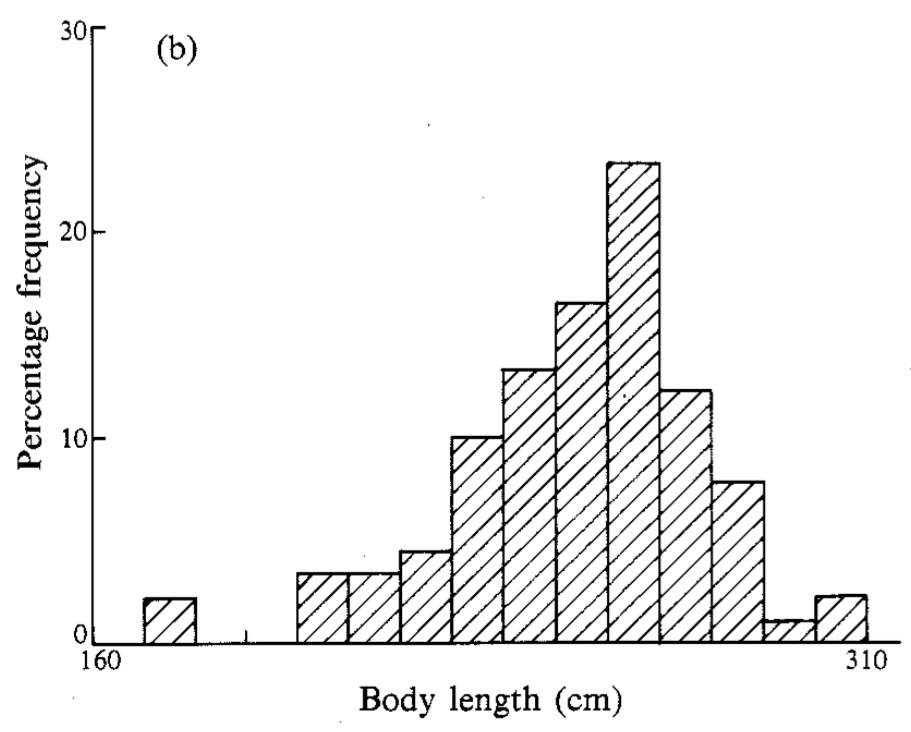
\includegraphics[width=0.55\linewidth]{ArticleImages/Bryden1984-Figure3b} 

}

\caption{A histogram of the body length of female Weddell seals}\label{fig:Bryden1984Fig3b}
\end{figure}

\section{\texorpdfstring{\textbf{Optional drills}: computational exercises}{Optional drills: computational exercises}}\label{Chapter3Drills}

\emph{(Answers appear in Sect. \ref{Lecture3Answers})}

\begin{drillBox}{iconmonstr-pencil-9-240.png}
These \emph{optional} \textbf{Drill} exercises (repeated practice) give you practice at getting computations correct, and using your calculator.
These drill questions are more about practising the underlying \emph{mathematics} rather than the \emph{statistics}.
If you need help, please \textbf{ask}.

\end{drillBox}

\begin{enumerate}
\def\labelenumi{\arabic{enumi}.}
\tightlist
\item
  The data in Table~\ref{tab:AISTable} give the heights of \(n = 7\) female tennis players at the \emph{Australian Institute of Sport} (AIS) in centimetres (\citeproc{ref-telford1991sex}{Telford and Cunningham 1991}).

  \begin{enumerate}
  \def\labelenumii{\alph{enumii}.}
  \tightlist
  \item
    Using your calculator's \emph{Statistics Mode}, find the \textbf{mean} and \textbf{standard deviation} of the data.
    \answerbox{2}
  \item
    Without using a calculator, find the \textbf{median} of the data.
    \answerbox{2}
  \item
    Compute the \textbf{IQR} for the data.
    \answerbox{2}
  \end{enumerate}
\end{enumerate}

\begin{table}
\centering
\caption{\label{tab:AISTable}The heights (in centimetres) of female tennis players at the AIS.}
\centering
\fontsize{10}{12}\selectfont
\begin{tabular}[t]{lllllll}
\toprule
$167.9$ & $177.5$ & $162.5$ & $172.5$ & $166.7$ & $175.0$ & $157.9$\\
\bottomrule
\end{tabular}
\end{table}

\begin{enumerate}
\def\labelenumi{\arabic{enumi}.}
\setcounter{enumi}{1}
\tightlist
\item
  Bamboo is a fast-growing, strong grass useful for environmentally-friendly building practices.
  A small research study explored the properties of bamboo when used as flooring material, including the bending strength (the Modulus of Rupture, or MOR, in MPa).
  Five different bamboo floorboards were provided by Bamboo Flooring Australia Pty Ltd and assessed by the Queensland Department of Primary Industries (\citeproc{ref-data:Gerber:BambooFlooring}{Gerber 2004}).
  The five MOR test results (in MPa) are shown in Table \ref{tab:MORTable}.

  \begin{enumerate}
  \def\labelenumii{\alph{enumii}.}
  \tightlist
  \item
    Identify the type of RQ being answered: descriptive, relational, cross-sectional or correlational.
    Justify your answer.
    \answerbox{2}
  \item
    Use your calculator's statistics mode to compute the \textbf{mean} and the \textbf{standard deviation}.
    \answerbox{2}
  \item
    Without using a calculator, find the \textbf{median} of the data.
    \answerbox{2}
  \end{enumerate}
\end{enumerate}

\begin{table}
\centering
\caption{\label{tab:MORTable}The MOR (in MPa) for five bamboo boards.}
\centering
\fontsize{10}{12}\selectfont
\begin{tabular}[t]{lllll}
\toprule
99.2 & 111.2 & 97.6 & 101.1 & 104\\
\bottomrule
\end{tabular}
\end{table}

\begin{enumerate}
\def\labelenumi{\arabic{enumi}.}
\setcounter{enumi}{2}
\tightlist
\item
  The data in Table~\ref{tab:AISTable2} give the percentage body fat of \(n = 9\) female swimmers at the \emph{Australian Institute of Sport} (AIS) (\citeproc{ref-telford1991sex}{Telford and Cunningham 1991}).

  \begin{enumerate}
  \def\labelenumii{\alph{enumii}.}
  \tightlist
  \item
    Using your calculator's \emph{Statistics Mode}, find the \textbf{mean} and \textbf{standard deviation} of the data.
  \item
    Without using a calculator, find the \textbf{median} of the data.
  \item
    Compute the \textbf{IQR}.
    \answerbox{4}
  \end{enumerate}
\end{enumerate}

\begin{table}
\centering
\caption{\label{tab:AISTable2}The percentage body fat of female swimmers at the AIS.}
\centering
\fontsize{10}{12}\selectfont
\begin{tabular}[t]{lllllllll}
\toprule
14.52 & 11.47 & 17.71 & 18.48 & 11.22 & 13.61 & 12.78 & 11.85 & 13.35\\
\bottomrule
\end{tabular}
\end{table}

\section{\texorpdfstring{\textbf{Optional questions}}{Optional questions}}\label{OptionalTW3}

\begin{optionalBox}{iconmonstr-help-4-240.png}
These questions are \textbf{optional}; e.g., if you need more practice, or you are studying for the exam.
(Answers appear in Sect.~\ref{Lecture3Answers}.)

\end{optionalBox}

\subsection{\texorpdfstring{\textbf{(Optional)} Using the calculator Statistics Mode}{(Optional) Using the calculator Statistics Mode}}\label{CalculatorBatteries}

Batteries are expensive, so comparing the performance of expensive and cheap batteries is helpful.
A test on the lifetime of batteries (\citeproc{ref-data:ALDIBatteryTesting}{Lindström 2011}) compared the time for two brands of \(1.5\)~volt batteries to reduce their voltage to \(1.0\)~volts under standard testing conditions.

The times (in hours) for nine Energizer Max batteries and nine ALDI brand batteries (Ultracell) are shown in Table~\ref{tab:BattTable}.

\begin{table}
\centering
\caption{\label{tab:BattTable}The times taken for batteries to go from $1.5\,\text{V}$ to $1.0\,\text{V}$, in hours.}
\centering
\fontsize{10}{12}\selectfont
\begin{tabular}[t]{>{}llllllllll}
\toprule
\textbf{Energizer} & $7.58$ & $7.46$ & $7.46$ & $7.59$ & $7.46$ & $7.52$ & $6.83$ & $6.89$ & $7.45$\\
\textbf{Ultracell} & $7.50$ & $7.48$ & $7.47$ & $7.48$ & $7.48$ & $7.41$ & $7.47$ & $6.96$ & $7.48$\\
\bottomrule
\end{tabular}
\end{table}

\begin{enumerate}
\def\labelenumi{\arabic{enumi}.}
\tightlist
\item
  Is the type of research study a true experimental, quasi-experimental, or observational study? Justify your answer.
  \tightlist
  \answerbox{2}
\item
  What are the \emph{units of observation} and \emph{units of analysis}?
  \answerbox{2}
\item
  Use your calculator's \emph{Statistics Mode} to compute the following. (Check your answers to ensure you are using your calculator correctly.)

  \begin{enumerate}
  \def\labelenumii{\alph{enumii}.}
  \item
    Compute the mean times for the \emph{Energizer} batteries (to two decimal places).
  \item
    Compute the standard deviation of the \emph{Energizer} battery times (to three decimal places).
  \item
    Compute the mean times for the \emph{Ultracell} batteries (to two decimal places).
  \item
    Compute the standard deviation of the \emph{Ultracell} battery times (to three decimal places).
  \end{enumerate}
\end{enumerate}

\answerbox{4}

\begin{enumerate}
\def\labelenumi{\arabic{enumi}.}
\setcounter{enumi}{3}
\tightlist
\item
  Explain what these calculations tell you.
  \answerbox{2}
\item
  Compute the median lifetime for each brand, explain what this tells you.
  (Many calculators cannot compute medians.)

  \begin{enumerate}
  \def\labelenumii{\alph{enumii}.}
  \item
    Compute the median of the \emph{Energizer} batteries (to two decimal places).
  \item
    Compute the median of the \emph{Ultracell} batteries (to two decimal places).
  \end{enumerate}
\end{enumerate}

\answerbox{3}

\begin{enumerate}
\def\labelenumi{\arabic{enumi}.}
\setcounter{enumi}{5}
\tightlist
\item
  Determine (and justify) if the mean or median would be a more appropriate measure of centre.
  \answerbox{2}
\item
  Do you think that the average time to reach \(1.0\)~volts is the same for each brand?
  Explain.
  \answerbox{2}
\item
  Information about the cost of the batteries would also be important information to know (see below).
  What advice would you give about buying batteries based on these data?
  \answerbox{2}
\end{enumerate}

\begin{tipBox}{iconmonstr-info-6-240.png}

The cost of the batteries, at the time of publication (05~September, 2012), was:

\begin{itemize}
\tightlist
\item
  \emph{Ultracell}: A four-pack cost \$2.49 from ALDI online
\item
  \emph{Energizer Max}: A four-pack cost \$5.97 from Woolworths online, \emph{on special}; the normal price was \$8.01 for the four-pack.
\end{itemize}

\end{tipBox}

\chapter{Teaching Week 4 tutorial}\label{Lecture4}

\begin{objectivesBox}{iconmonstr-target-4-240.png}

You will learn to:

\begin{itemize}
\tightlist
\item
  produce and understand graphical summaries for \textbf{qualitative} data.
\item
  produce and understand numerical summaries for \textbf{qualitative} data (e.g., odds, proportions).
\item
  produce and understand graphical summaries for comparing \textbf{qualitative} data.
\item
  produce and understand numerical summaries for comparing \textbf{qualitative} data (e.g., odds ratios, difference in proportions).
\end{itemize}

\end{objectivesBox}

\begin{assessmentBox}{iconmonstr-text-check-list-lined-240.png}

The Week~4 content is essential for:

\begin{itemize}
\tightlist
\item
  \textbf{Task~2A}, which requires you to \emph{suggest appropriate numerical summaries, and suggest appropriate graphs};
\item
  \textbf{Task~2B}, which requires you to \emph{produce and interpret appropriate numerical summaries and produce and interpret appropriate graphs};
\item
  \textbf{Quiz~2}, which includes questions about \emph{numerical summaries and graphs}; and
\item
  the \textbf{Exam}, which will contain questions about \emph{numerical summaries and graphs}.
\end{itemize}

\end{assessmentBox}

\begin{readBox}{iconmonstr-school-15-240.png}
You will learn and practice the content associated with these chapters of the \href{https://peterkdunn.github.io/SRM-Textbook/}{textbook}:

\begin{itemize}
\tightlist
\item
  \href{https://peterkdunn.github.io/SRM-Textbook/SummariseQualData.html}{Chapter~12 (Summarising qualitative data)}.
\item
  \href{https://peterkdunn.github.io/SRM-Textbook/CompareQualData.html}{Chapter~15 (Comparing qualitative data between individuals}.
\end{itemize}

Take careful note of which chapters are covered in this tutorial!

\end{readBox}

\begin{tipBox}{iconmonstr-info-6-240.png}
You should bring your calculator to tutorials from this week onwards.

\end{tipBox}

\pagebreak

\section{Quick revision}\label{QuickRevision-Tutorial4}

A study of obstructive sleep apnoea (OSA) in adults with Down Syndrome (\citeproc{ref-carvalho2020stop}{{de Carvalho et al.} 2020}) had \(n = 60\) adults (\(27\)~females; \(33\)~males) undergo a sleep study.
Part of the data are in Table~\ref{tab:OSAKable3}.
(REI is the Respiratory Event Index; an REI under~\(5\) refers to no sleep apnoea; an REI of \(30\)~or over refers to severe sleep apnoea.)

\begin{enumerate}
\def\labelenumi{\arabic{enumi}.}
\tightlist
\item
  Which of these would be an \textbf{inappropriate} numerical summary for the age of the participants? \tightlist  

  \begin{enumerate}
  \def\labelenumii{\alph{enumii}.}
  \tightlist
  \item
    Median.
  \item
    Odds.
  \item
    Standard deviation.
  \item
    Mean.
  \end{enumerate}
\item
  What might be an \textbf{appropriate} way to numerically describe the amount of \emph{variation} in the ages of participants?

  \begin{enumerate}
  \def\labelenumii{\alph{enumii}.}
  \tightlist
  \item
    Standard deviation.
  \item
    Median.
  \item
    Mean.
  \item
    Odds.
  \end{enumerate}
\item
  What might be an \textbf{appropriate} way to numerically describe the average Respiratory Event Index (REI) of participants?

  \begin{enumerate}
  \def\labelenumii{\alph{enumii}.}
  \tightlist
  \item
    Percentage.
  \item
    Odds.
  \item
    Standard deviation.
  \item
    Mean.
  \end{enumerate}
\item
  What might be an \textbf{appropriate} way to numerically describe the gender of the participants?

  \begin{enumerate}
  \def\labelenumii{\alph{enumii}.}
  \tightlist
  \item
    Standard deviation.
  \item
    Median.
  \item
    IQR.
  \item
    Percentages.
  \end{enumerate}
\item
  In the sample of \(n = 60\), what \textbf{percentage} of individuals are females?

  \begin{enumerate}
  \def\labelenumii{\alph{enumii}.}
  \tightlist
  \item
    \begin{enumerate}
    \def\labelenumiii{\arabic{enumiii}.}
    \setcounter{enumiii}{121}
    \tightlist
    \item
    \end{enumerate}
  \item
    0.82.
  \item
    0.45.
  \item
    45\%.
  \item
    55\%.
  \item
    0.55.
  \end{enumerate}
\item
  In the sample of \(n = 60\), what are the \textbf{odds} that an individual is female?

  \begin{enumerate}
  \def\labelenumii{\alph{enumii}.}
  \tightlist
  \item
    0.45.
  \item
    45\%.
  \item
    \begin{enumerate}
    \def\labelenumiii{\arabic{enumiii}.}
    \setcounter{enumiii}{121}
    \tightlist
    \item
    \end{enumerate}
  \item
    55\%.
  \item
    0.55.
  \item
    0.82.
  \end{enumerate}
\item
  Use the jamovi output in Fig.~\ref{fig:OSAoutput} to find the mean of \emph{Gender}, and explain what this means.
  \answerbox{3}
\end{enumerate}

\begin{figure}[hbtp]

{\centering 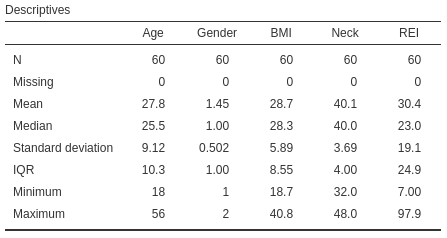
\includegraphics[width=0.75\linewidth]{SoftwareImages/OSADescriptive} 

}

\caption{A numerical summary of the OSA data: jamovi}\label{fig:OSAoutput}
\end{figure}

\begin{table}
\centering
\caption{\label{tab:OSAKable3}Part of the Obstructive Sleep Apnoea (OSA) data set.}
\centering
\fontsize{10}{12}\selectfont
\begin{tabular}[t]{ccccc}
\toprule
\textbf{Age} & \textbf{Gender} & \textbf{BMI} & \textbf{Neck circumference (cm)} & \textbf{REI}\\
\midrule
21 & Male & 20.3 & 37 & 46\\
24 & Male & 24.1 & 40.5 & 19.3\\
26 & Male & 25.2 & 38 & 12.4\\
39 & Female & 40.8 & 41 & 58.6\\
21 & Female & 35 & 37 & 12.7\\
\addlinespace
29 & Male & 29.2 & 41 & 38.8\\
20 & Male & 25.8 & 42 & 24.4\\
21 & Male & 20.9 & 37 & 7\\
19 & Female & 20.5 & 32 & 37.6\\
27 & Male & 22.4 & 39 & 21.7\\
\addlinespace
$\vdots$ & $\vdots$ & $\vdots$ & $\vdots$ & $\vdots$\\
\bottomrule
\end{tabular}
\end{table}

\section{Class discussion}\label{TW4-Class-Discussion}

\begin{discussBox}{iconmonstr-speech-bubble-26-240.png}
\textbf{Discuss}: The raw data is more useful than a graphical summary.

\end{discussBox}

\section{Percentages and odds}\label{PercentOddsStroke}

In a study of how well emergency dispatchers recognised signs of stroke (\citeproc{ref-oostema2018emergency}{Oostema et al. 2018}), the data in Table~\ref{tab:Stroke} were collected.

\begin{table}
\centering
\caption{\label{tab:Stroke}How well emergency dispatchers recognised signs of stroke.}
\centering
\fontsize{10}{12}\selectfont
\begin{tabular}[t]{>{}lcc}
\toprule
\multicolumn{1}{c}{\textbf{ }} & \multicolumn{1}{c}{\textbf{Dispatcher}} & \multicolumn{1}{c}{\textbf{Dispatcher}} \\
\textbf{ } & \textbf{suspected stroke} & \textbf{missed stroke}\\
\midrule
\textbf{Males} & 67 & 43\\
\textbf{Females} & 97 & 39\\
\bottomrule
\end{tabular}
\end{table}

\begin{enumerate}
\def\labelenumi{\arabic{enumi}.}
\tightlist
\item
  \emph{Why} are the levels `Male' and `Female' placed in the rows of the table, rather than the columns?
  \answerbox{2}
\item
  What proportion of patients had their stroke symptoms missed? \tightlist
  \answerbox{2}
\item
  Sketch a side-by-side or stacked bar chart to display the data.
  \answerbox{4}
\item
  Of the \emph{male} patients, what \emph{proportion} had their stroke symptoms missed by the dispatcher?
  \null
  \answerbox{2}
\item
  Of the \emph{female} patients, what \emph{proportion} had their stroke symptoms missed by the dispatcher?
  \null
  \answerbox{2}
\item
  For the \emph{male} patients, what are the \emph{odds} that they had their stroke symptoms missed by the dispatcher?
  \null
  \answerbox{2}
\item
  For the \emph{female} patients, what are the \emph{odds} that they had their stroke symptoms missed by the dispatcher?
  \null
  \answerbox{2}
\item
  What is the \emph{difference between the proportions} of stroke symptoms being missed by the dispatcher, comparing \emph{males} to \emph{females}?
  \null
  \answerbox{2}
\item
  What is the \emph{odds ratio} that a patients had their stroke symptoms missed by the dispatcher, comparing \emph{males} to \emph{females}?
  \null
  \answerbox{2}
\item
  Construct a numerical summary table by completing Table~\ref{tab:StrokeSymptomsSummary}.
\end{enumerate}

\begin{table}
\centering
\caption{\label{tab:StrokeSymptomsSummary}Numerical summary table: emergency dispatchers and missing stroke symptoms.}
\centering
\fontsize{10}{12}\selectfont
\begin{tabular}[t]{l|c|c|c}
\hline
\multicolumn{1}{c|}{\textbf{ }} & \multicolumn{1}{c|}{\textbf{Proportion of}} & \multicolumn{1}{c|}{\textbf{Odds that}} & \multicolumn{1}{c}{\textbf{Sample}} \\
\textbf{ } & \textbf{symptoms missed} & \textbf{symptoms missed} & \textbf{size}\\
\hline
Males & \null & \null & \null\\
 
\null & \null & \null & \vphantom{2} \null\\
\hline
Females & \null & \null & \null\\
 
\null & \null & \null & \vphantom{1} \null\\
\hline
\null & \multicolumn{1}{l|}{\em{Difference:\hspace{4cm}\null }} & \multicolumn{1}{l|}{\em{Odds ratio:\hspace{4cm}\null }} & \null\\
 
\null & \null & \null & \null\\
\hline
\end{tabular}
\end{table}

\section{Two-way tables}\label{TwoWayTables}

Soccer (football) is a unique in that one aspect is `the purposeful use of the unprotected head for controlling and advancing the ball' (\citeproc{ref-kirkendall2001heading}{Kirkendall et al. 2001}).
Some researchers suspect that repeatedly `heading' the ball may impair brain function.

A study (\citeproc{ref-kirkendall2001heading}{Kirkendall et al. 2001}) was conducted to determine (p.~157)

\begin{quote}
\ldots whether long-term or chronic neuropsychological dysfunction (i.e.~concussion) was present in collegiate soccer players\ldots{}
\end{quote}

Data were collected from \(240\)~college students for two variables:

\begin{itemize}
\tightlist
\item
  The student type: one of `soccer player', `non-soccer athlete', or `non-athlete'.
\item
  The number of head concussions: each student was asked about the number of head concussions they had experienced; `zero' , `one', or `two or more' concussions.
\end{itemize}

Use the study data (Table~\ref{tab:SoccerTable}) to answer the following questions.

\begin{table}
\centering
\caption{\label{tab:SoccerTable}Data on concussions experienced by college students.}
\centering
\fontsize{10}{12}\selectfont
\begin{tabular}[t]{>{}lccc>{}c}
\toprule
\multicolumn{1}{c}{\textbf{ }} & \multicolumn{3}{c}{\textbf{Num. concussions}} & \multicolumn{1}{c}{\textbf{ }} \\
\cmidrule(l{3pt}r{3pt}){2-4}
\textbf{ } & \textbf{0} & \textbf{1} & \textbf{2 or more} & \textbf{Total}\\
\midrule
\textbf{Soccer players} & $\phantom{0}45$ & $\phantom{0}\phantom{0}5$ & $\phantom{0}13$ & \textbf{$\phantom{0}63$}\\
\textbf{Non-soccer athletes} & $\phantom{0}68$ & $\phantom{0}25$ & $\phantom{0}\phantom{0}3$ & \textbf{$\phantom{0}96$}\\
\textbf{Non-athletes} & $\phantom{0}45$ & $\phantom{0}15$ & $\phantom{0}21$ & \textbf{$\phantom{0}81$}\\
\midrule
\textbf{\textbf{Total}} & \textbf{$158$} & \textbf{$\phantom{0}45$} & \textbf{$\phantom{0}37$} & \textbf{\textbf{$240$}}\\
\bottomrule
\end{tabular}
\end{table}

\begin{enumerate}
\def\labelenumi{\arabic{enumi}.}
\tightlist
\item
  \emph{Why} is the number of concussions placed in the columns of the table, rather than the rows?
  \answerbox{2}
\item
  Classify the two variables.
  \answerbox{2}
\item
  Compute the percentage of college students in the \emph{sample} that have received exactly one concussion.
  \answerbox{2}
\item
  Compute the percentage of college students in the population that have received two or more concussions.
  \answerbox{2}
\item
  Many possible graphs exists to display the data; four are shown in Fig.~\ref{fig:SoccerGraph}.
  What is the main message from each graph?
  Which graph do you think is best?
  Why?
  \answerbox{2}
\item
  Among \textbf{non-athletes}, compute the odds of receiving two or more concussions.
  Interpret what this means.
  \answerbox{2}
\item
  Among \textbf{soccer players}, compute the odds of receiving two or more concussions.
  Interpret what this means.
  \answerbox{2}
\item
  Compute the odds ratio comparing the odds of a non-athlete receiving two or more concussions to the odds of a soccer player receiving two or more concussions.
  \answerbox{2}
\item
  Create a table of \textbf{column} percentages.
  What do these tell you?
  \answerbox{4}
\item
  Create a table of \textbf{row} percentages.
  What do these tell you?
  \answerbox{4}
\item
  Which one of these tables is probably more sensible?
  Why?
  \answerbox{2}
\item
  What did you learn from this study?
  \answerbox{2}
\end{enumerate}

\begin{figure}[hbtp]

{\centering 
\includegraphics[width=0.75\linewidth]{04-TW4-Tutorial_files/figure-latex/SoccerGraph-1} 

}

\caption{Four different graphs displaying the soccer-data. 'S' mean a soccer player; 'NS' means a non-soccer athlete; 'NA' means a non-athlete.}\label{fig:SoccerGraph}
\end{figure}

\pagebreak

\section{Working with odds}\label{WorkingWithOdds}

A study (\citeproc{ref-data:montalvo2020:retrospective}{Montalvo et al. 2020}) examined \(433\)~bridge collapses.
Of these \(433\)~bridges, \(36\)~bridges collapsed due to deterioration, and \(82\)~bridges collapsed due to a collision.

\begin{enumerate}
\def\labelenumi{\arabic{enumi}.}
\item
  The \textbf{percentage} of bridges collapsing due to deterioration is \_\_\_\_\_ divided by \_\_\_\_\_, or~\(8.3\)\%.
\item
  The \textbf{odds} of a bridge collapsing due to deterioration is \_\_\_\_\_ divided by \_\_\_\_\_, or~\(0.091\).
\item
  The odds of a bridge collapsing due to deterioration is~\(0.091\).
  What does this mean?

  \begin{enumerate}
  \def\labelenumii{\alph{enumii}.}
  \tightlist
  \item
    For every \(100\) bridges that do collapse due to deterioration, about \(9.1\) bridges do not collapse.
  \item
    For every \(100\) bridges that do not collapse due to deterioration, about \(9.1\) bridges do collapse.
  \item
    About \(9\)\% of bridges collapse due to deterioration.
  \item
    About \(90\)\% of bridges collapse due to deterioration.
  \end{enumerate}
\item
  The percentage of bridges \textbf{not} collapsing due to deterioration is \_\_\_\_\_ divided by \_\_\_\_\_, or \(91.7\)\%.
\item
  The odds of a bridge \textbf{not} collapsing due to deterioration is \_\_\_\_\_ divided by \_\_\_\_\_, or \(11.0\).
\item
  The percentage of bridge collapses due to collisions is \_\_\_\_\_ divided by \_\_\_\_\_, or \(18.9\)\%.
\item
  The odds of a bridge collapsing due to collisions is \_\_\_\_\_ divided by \_\_\_\_\_, or \(0.234\).
\item
  True or false: The odds of an event cannot be larger than one.
\item
  True or false: The odds of an event cannot be smaller than one.
\item
  Which \textbf{one} of the following statements is true?

  \begin{enumerate}
  \def\labelenumii{\alph{enumii}.}
  \tightlist
  \item
    Proportions and odds are the same thing.
  \item
    Percentages must be whole numbers.
  \item
    Odds cannot be negative
  \end{enumerate}
\end{enumerate}

\section{\texorpdfstring{\textbf{Optional drills}: Computational exercises}{Optional drills: Computational exercises}}\label{Chapter4Drills}

\emph{(Answers appear in Sect. \ref{Lecture4Answers})}

\begin{drillBox}{iconmonstr-pencil-9-240.png}
These \emph{optional} \textbf{Drill} exercises (repeated practice) give you practice at getting computations correct, and using your calculator.
These drill questions are more about practising the underlying \emph{mathematics} rather than the \emph{statistics}.
If you need help, please \textbf{ask}.

\end{drillBox}

\begin{enumerate}
\def\labelenumi{\arabic{enumi}.}
\item
  A study of drivers (\citeproc{ref-data:mcevoy2006:phoneuse}{McEvoy et al. 2006}) in New South Wales (NSW) and Western Australia (WA) were asked if they use their phone while driving (Table \ref{tab:PDTable}).

  \begin{enumerate}
  \def\labelenumii{\alph{enumii}.}
  \tightlist
  \item
    What \textbf{percentage} of people use their phone while driving?
    \answerbox{1}
  \item
    What are the \textbf{odds} that a person uses their phone while driving?
    \answerbox{1}
  \item
    What are the \textbf{odds} that a WA resident uses their phone while driving?
    \answerbox{1}
  \item
    What are the \textbf{odds} that a NSW resident uses their phone while driving?
    \answerbox{1}
  \item
    What are the \textbf{odds ratio} that a person uses their phone while driving, comparing WA residents to NSW residents?
    \answerbox{2}
  \end{enumerate}
\end{enumerate}

\begin{table}
\centering
\caption{\label{tab:PDTable}The number of drivers who use their phone while driving.}
\centering
\fontsize{10}{12}\selectfont
\begin{tabular}[t]{>{}lcc}
\toprule
\textbf{ } & \textbf{Uses phone} & \textbf{Does not use phone}\\
\midrule
\textbf{NSW} & 381 & 295\\
\textbf{WA} & 345 & 326\\
\bottomrule
\end{tabular}
\end{table}

\begin{enumerate}
\def\labelenumi{\arabic{enumi}.}
\setcounter{enumi}{1}
\tightlist
\item
  The data in Table \ref{tab:RSTable} give the number of plum cuttings that were alive or dead, and whether the rootstock was long or short (\citeproc{ref-bartlett1935contingency}{Bartlett 1935}).

  \begin{enumerate}
  \def\labelenumii{\alph{enumii}.}
  \tightlist
  \item
    Compute the \textbf{percentage} of cuttings that were \emph{alive} at the end of the study.
    \answerbox{1}
  \item
    Compute the \textbf{percentage} of cuttings that were \emph{dead} at the end of the study.
    \answerbox{1}
  \item
    Compute the \textbf{percentage} of cuttings that were \emph{long}.
    \answerbox{1}
  \item
    Compute the \textbf{odds} that a cuttings was \emph{alive} at the end of the study.
    \answerbox{1}
  \item
    Compute the \textbf{odds} that a cuttings was \emph{alive} at the end of the study, only for the \emph{long} cuttings.
    \answerbox{1}
  \item
    Compute the \textbf{odds} that a cuttings was \emph{alive} at the end of the study, only for the \emph{short} cuttings.
    \answerbox{1}
  \item
    Compute the \textbf{odds ratio} that a cutting was \emph{alive} at the end of the study, comparing the \emph{short} cuttings to the \emph{long} cuttings.
    \answerbox{1}
  \end{enumerate}
\end{enumerate}

\begin{table}
\centering
\caption{\label{tab:RSTable}The relationship between length and condition of plum rootstocks.}
\centering
\fontsize{10}{12}\selectfont
\begin{tabular}[t]{>{}lrr}
\toprule
\textbf{ } & \textbf{Alive} & \textbf{Dead}\\
\midrule
\textbf{Long} & 240 & 240\\
\textbf{Short} & 138 & 342\\
\bottomrule
\end{tabular}
\end{table}

\section{\texorpdfstring{\textbf{Optional questions}}{Optional questions}}\label{OptionalTW4}

\begin{optionalBox}{iconmonstr-help-4-240.png}
These questions are \textbf{optional}; e.g., if you need more practice, or you are studying for the exam.
(Answers appear in Sect.~\ref{Lecture4Answers}.)

\end{optionalBox}

\subsection{\texorpdfstring{\textbf{(Optional)} Odds ratios}{(Optional) Odds ratios}}\label{OddsRatioSMND}

\begin{videoSolutionBox}{iconmonstr-youtube-10-240.png}
This question has a video solution in the online book, so you can hear and see the solution.

\end{videoSolutionBox}

The impact of environmental toxins is not well understood.
Pamphlett (\citeproc{ref-data:Pamphlett:toxins}{2012}) examined the association between the environmental exposure of toxins and sporadic motor neuron disease (SMND).
A total of \(380\)~SMND cases and \(377\) controls were studied.
Of the \(380\)~SMND cases, \(60\) had worked with metal in the past; of the \(377\) controls, \(33\) had worked with metal in the past.

\begin{enumerate}
\def\labelenumi{\arabic{enumi}.}
\tightlist
\item
  What is the \emph{direction} of this study?
  \answerbox{1}
\item
  Construct a two-way table showing the relationship between disease group, and whether not the specific person had worked with metal, in the sample.
  \answerbox{4}
\item
  Using your table, compute the \emph{odds} that a person \emph{with} SMND had worked with metal.
  Interpret what this means.
  \answerbox{2}
\item
  Using your table, compute the \emph{odds} that a person \emph{without} SMND had worked with metal.
  Interpret what this means.
  \answerbox{2}
\item
  How many times greater is the odds that a person \emph{with} SMND having worked with metal, compared to the odds that a person \emph{without} SMND having worked with metal?
  (This is an \emph{odds ratio}.)
  \answerbox{2}
\item
  Using your table, compute the \emph{percentage} of people \emph{with} SMND that had worked with metal.
  \answerbox{1}
\item
  Using your table, compute the \emph{percentage} of people \emph{without} SMND that had worked with metal.
  \answerbox{1}
\item
  A newspaper report states SMND rates are almost the same between those worked with metal and those who did not.
  Do you agree or disagree?
  \answerbox{1}
\item
  Sketch a bar chart to display the data.
  \answerbox{4}
\end{enumerate}

\chapter{Teaching Week 5 tutorial}\label{Lecture5}

\begin{objectivesBox}{iconmonstr-target-4-240.png}

You will learn to produce and understand:

\begin{itemize}
\tightlist
\item
  graphical summaries for \emph{between}-individuals comparisons for \textbf{quantitative} data.
\item
  numerical summaries for \emph{between}-individuals comparisons for \textbf{quantitative} data.
\item
  graphical summaries for \emph{within}-individuals comparisons for \textbf{quantitative} data.
\item
  numerical summaries for \emph{within}-individuals comparisons for \textbf{quantitative} data.
\item
  graphical summaries for correlational studies.
\item
  numerical summaries for correlational studies.
\end{itemize}

\end{objectivesBox}

\begin{assessmentBox}{iconmonstr-text-check-list-lined-240.png}

The Week~5 content is essential for:

\begin{itemize}
\tightlist
\item
  \textbf{Task~2B}, which requires you to \emph{produce appropriate numerical summaries and produce appropriate graphs};
\item
  \textbf{Quiz~2}, which includes questions about \emph{numerical summaries and graphs}; and
\item
  the \textbf{Exam}, which will contain questions about \emph{numerical summaries and graphs}.
\end{itemize}

\end{assessmentBox}

\begin{readBox}{iconmonstr-school-15-240.png}
You will learn and practice the content associated with these chapters of the \href{https://peterkdunn.github.io/SRM-Textbook/}{textbook}:

\begin{itemize}
\tightlist
\item
  \href{https://peterkdunn.github.io/SRM-Textbook/SummariseWithin.html}{Chapter 13 (Comparing quantitative data within individuals)}.
\item
  \href{https://peterkdunn.github.io/SRM-Textbook/BetweenQuantData.html}{Chapter 14 (Comparing quantitative data between individuals)}.
\item
  \href{https://peterkdunn.github.io/SRM-Textbook/TwoQuant.html}{Chapter 16 (Correlations between quantitative variables)}.
\item
  \href{https://peterkdunn.github.io/SRM-Textbook/SummariseComments.html}{Chapter 17 (More details about tables and graphs)}.
\end{itemize}

Take careful note of which chapters are covered in this tutorial!

\end{readBox}

\pagebreak

\section{Quick revision}\label{QuickRevision-Tutorial5}

Lunn and McNeil (\citeproc{ref-others:lunn:cida}{1991}) compared the dimensions of jellyfish at two sites at Hawkesbury River, NSW (Dangar Island; Salamander Bay) to determine the difference between the jellyfish at each site.
A histogram of the breadth of jellyfish at Dangar Island Bay is shown in Fig.~\ref{fig:JellyfishHist}.

\begin{figure}[hbtp]

{\centering 
\includegraphics[width=0.5\linewidth]{05-TW5-Tutorial_files/figure-latex/JellyfishHist-1} 

}

\caption{A histogram of the breadth of jellyfish at Dangar Island.}\label{fig:JellyfishHist}
\end{figure}

\begin{enumerate}
\def\labelenumi{\arabic{enumi}.}
\tightlist
\item
  Two students are arguing about the median breadth.
  Who is correct?
  Why?

  \begin{enumerate}
  \def\labelenumii{\alph{enumii}.}
  \tightlist
  \item
    Student 1.
  \item
    Student 2.
  \item
    Neither is correct.
  \item
    Both are correct.
  \end{enumerate}
\end{enumerate}

\textbf{Student~1} says:

\begin{quote}
The bars in the histogram have heights of \(10\), \(2\), \(4\), \(2\) and \(4\).
When these numbers are put in order, they are: \(2\), \(2\), \(4\), \(4\), \(10\).
The median breadth is the median of these numbers, so the median breadth is the middle one: \(4\,\text{mm}\) is the median.
\end{quote}

\textbf{Student~2} responds:

\begin{quote}
You have the correct answer, but for the wrong reason!
There are five bars, and the middle bar is the third bar.
Since the third bar has a height of \(4\), the median breadth is \(4\,\text{mm}\).
\end{quote}

\answerbox{2}

\begin{enumerate}
\def\labelenumi{\arabic{enumi}.}
\setcounter{enumi}{1}
\tightlist
\item
  Describe the histogram.
  \answerbox{2}
\item
  A boxplot comparing the breadths of jellyfish at Dangar Island and Salamander Bay is shown in Fig.~\ref{fig:JellyfishBoxplots}.
  Describe and compare the breadths of the jellyfish.
  \answerbox{3}
\item
  Which box in the boxplot represents the Dangar Island jellyfish (shown in Fig.~\ref{fig:JellyfishHist})?
  \answerbox{1}
\item
  The difference between means was defined as \(\mu_A - \mu_B\) (where \(\mu_A\) is the mean breadth at Site~A, and \(\mu_B\) is the mean breadth at Site~B).
  What would a value of \(-6.0\,\text{mm}\) mean?
  \answerbox{2}
\item
  What did you learn from this study?
  \answerbox{1}
\end{enumerate}

\begin{figure}[hbtp]

{\centering 
\includegraphics[width=0.5\linewidth]{05-TW5-Tutorial_files/figure-latex/JellyfishBoxplots-1} 

}

\caption{A boxplot of the breadth of jellyfish at two sites.}\label{fig:JellyfishBoxplots}
\end{figure}

\section{Class discussion}\label{TW5-Class-Discussion}

\begin{discussBox}{iconmonstr-speech-bubble-26-240.png}
\textbf{Discuss}: A badly designed experiment with lots of data is worse than a small, well-designed one.

\end{discussBox}

\section{Critiquing students' numerical summaries}\label{CritiqueStudentSummaries}

In this activity, you get to critique actual student Project submissions, so you can critique your own \emph{before} submission.

\begin{enumerate}
\def\labelenumi{\arabic{enumi}.}
\item
  Critique the numerical summary in Fig.~\ref{fig:StudentsNumSumA}, a screenshot from a student Project Report.
  Identify ways to improve the numerical summary.

  The RQ is `\emph{What is the mean difference between the kicking distance using dominant and non-dominant legs?}'
\end{enumerate}

\begin{importantBox}{iconmonstr-warning-8-240.png}
You don't know what `standard error' means yet, so don't worry about that column.

\end{importantBox}

\answerbox{4}

\begin{figure}[hbtp]

{\centering 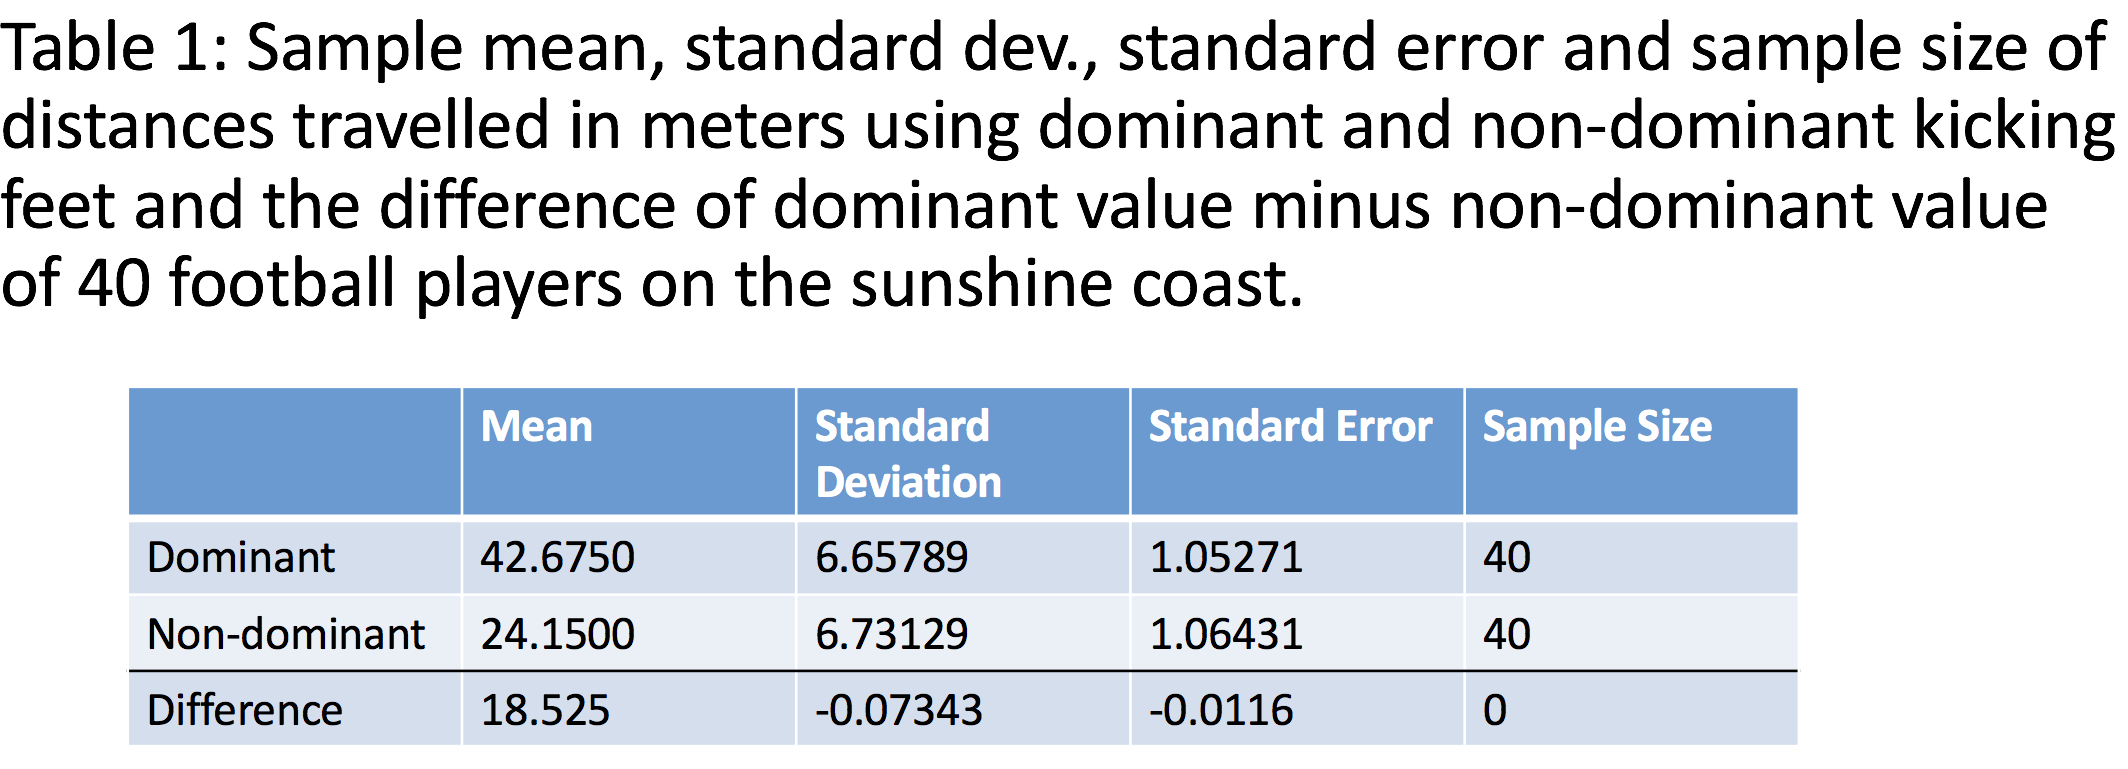
\includegraphics[width=0.7\linewidth]{ProjectImages/StudentResults1} 

}

\caption{A numerical summary from a student Project.}\label{fig:StudentsNumSumA}
\end{figure}

\begin{enumerate}
\def\labelenumi{\arabic{enumi}.}
\setcounter{enumi}{1}
\item
  Critique the numerical summary in Fig.~\ref{fig:StudentsNumSumChiA}, a screenshot from a student Project Report.
  Identify ways to improve the numerical summary.

  The RQ is `\emph{Is there a difference between the proportions of drink orders that are for coffee (rather than non-coffee) comparing the morning and the afternoon?}'
\end{enumerate}

\begin{figure}[hbtp]

{\centering 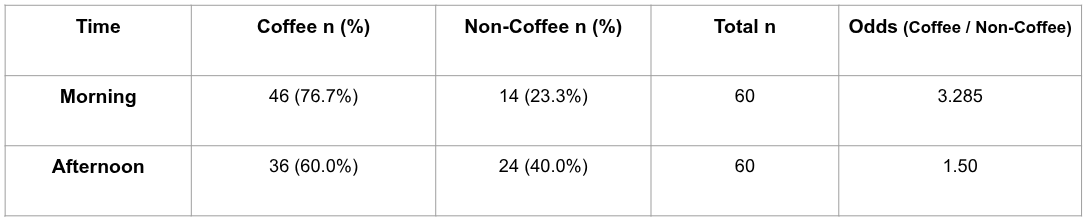
\includegraphics[width=1\linewidth]{ProjectImages/NumericalSummaryChi2} 

}

\caption{A numerical summary from a student Project.}\label{fig:StudentsNumSumChiA}
\end{figure}

Make some notes about important things you learnt from this activity, to remember when creating your numerical summaries for Task~2B.
\answerbox{3}

\section{Critiquing students' graphs}\label{CritiqueStudentGraphs1}

In this activity, you get to critique actual SCI110 Project submissions, so you can critique your own \emph{before} submission.

\begin{enumerate}
\def\labelenumi{\arabic{enumi}.}
\tightlist
\item
  Critique the graph in Fig.~\ref{fig:StudentsGraphsA}, a screenshot from a student Project Report comparing the average burn time between two brands of sparklers.
  \answerbox{4}
\end{enumerate}

\begin{figure}[hbtp]

{\centering 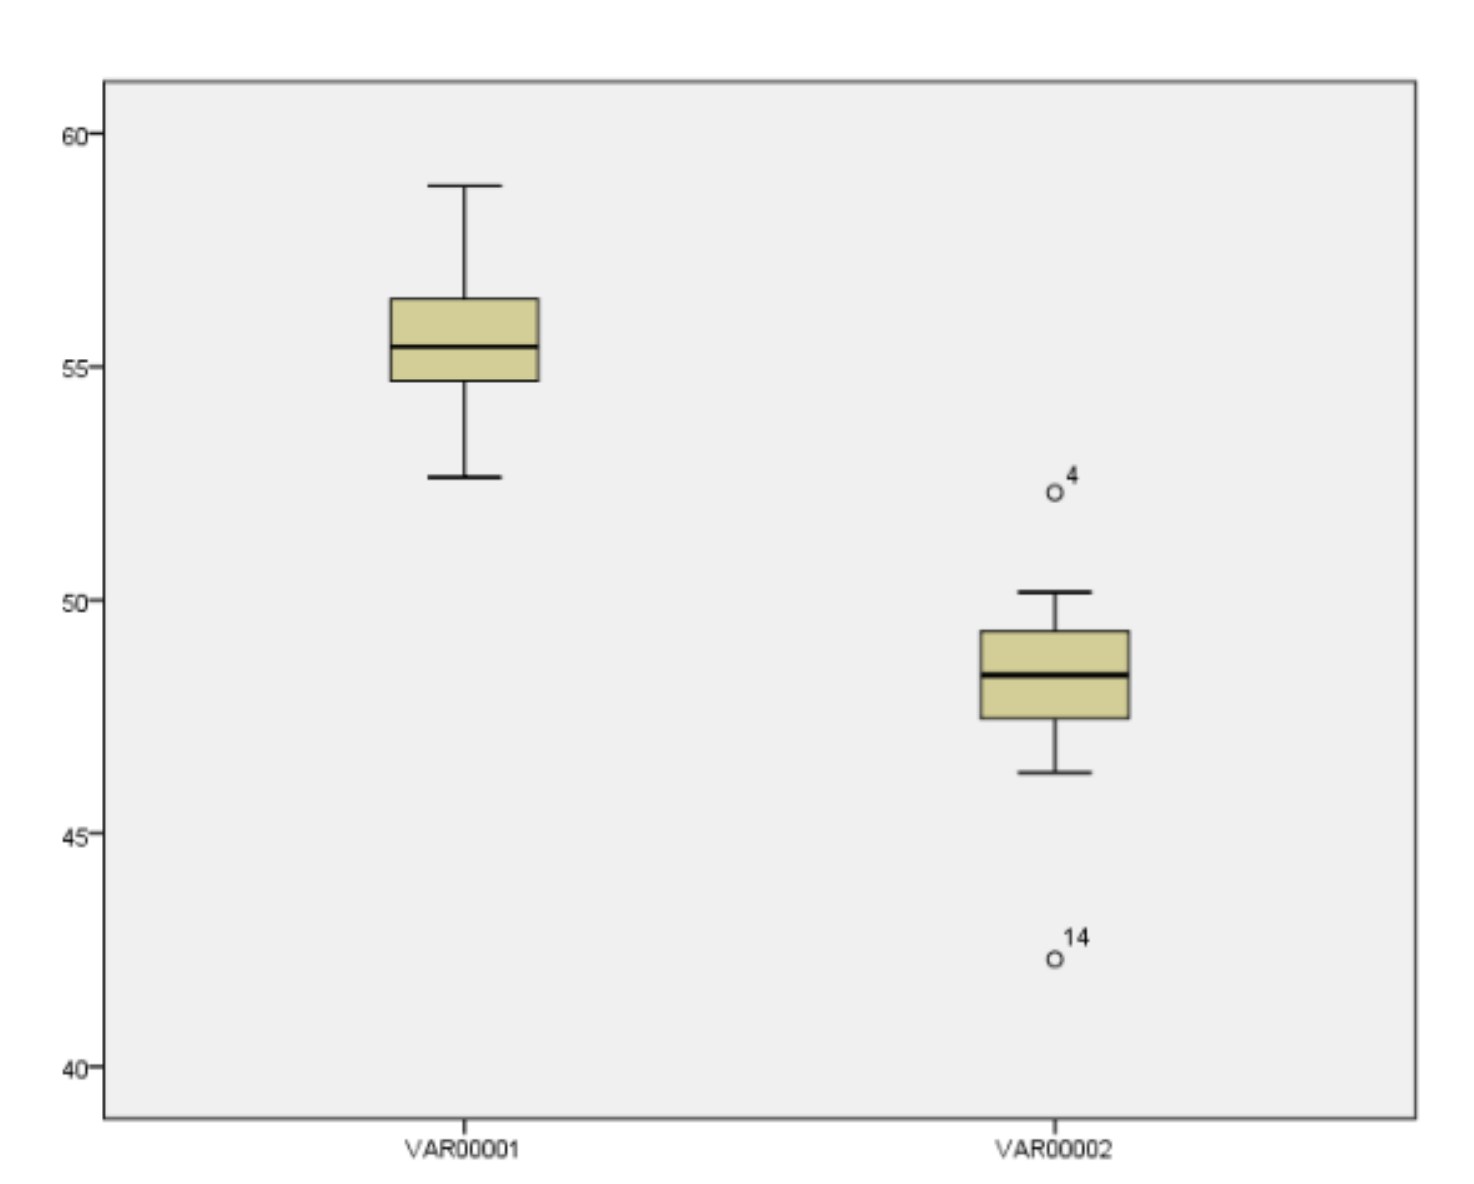
\includegraphics[width=0.7\linewidth]{ProjectImages/BareBoxplot} 

}

\caption{A graph from a student Project.}\label{fig:StudentsGraphsA}
\end{figure}

\begin{enumerate}
\def\labelenumi{\arabic{enumi}.}
\setcounter{enumi}{1}
\tightlist
\item
  Critique the graph in Fig.~\ref{fig:StudentsGraphsChiB}, a screenshot from a student Project Report comparing the percentage of students at UniSC wearing grey-scale clothing between females and males.
  \answerbox{4}
\end{enumerate}

\begin{figure}[hbtp]

{\centering 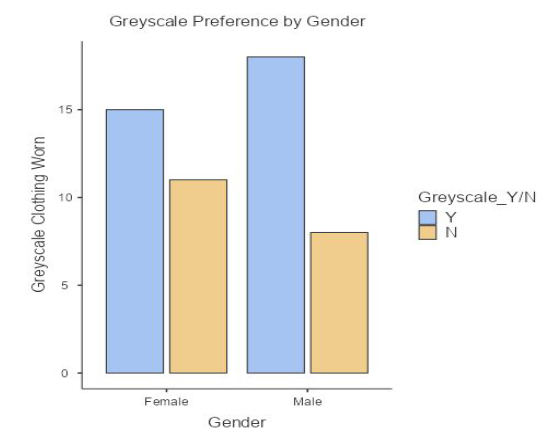
\includegraphics[width=0.65\linewidth]{ProjectImages/GraphicalSummaryChi2} 

}

\caption{A graph from a student Project.}\label{fig:StudentsGraphsChiB}
\end{figure}

\begin{enumerate}
\def\labelenumi{\arabic{enumi}.}
\setcounter{enumi}{2}
\tightlist
\item
  Critique the graph in Fig.~\ref{fig:StudentsGraphsC}, a screenshot from a student Project Report comparing the `mean dissolve' time (they probably meant `mean \emph{dissolving} time') of Panadol in room temperature and cold water.
  Identify ways to improve the graph.
  \answerbox{4}
\end{enumerate}

\begin{figure}[hbtp]

{\centering 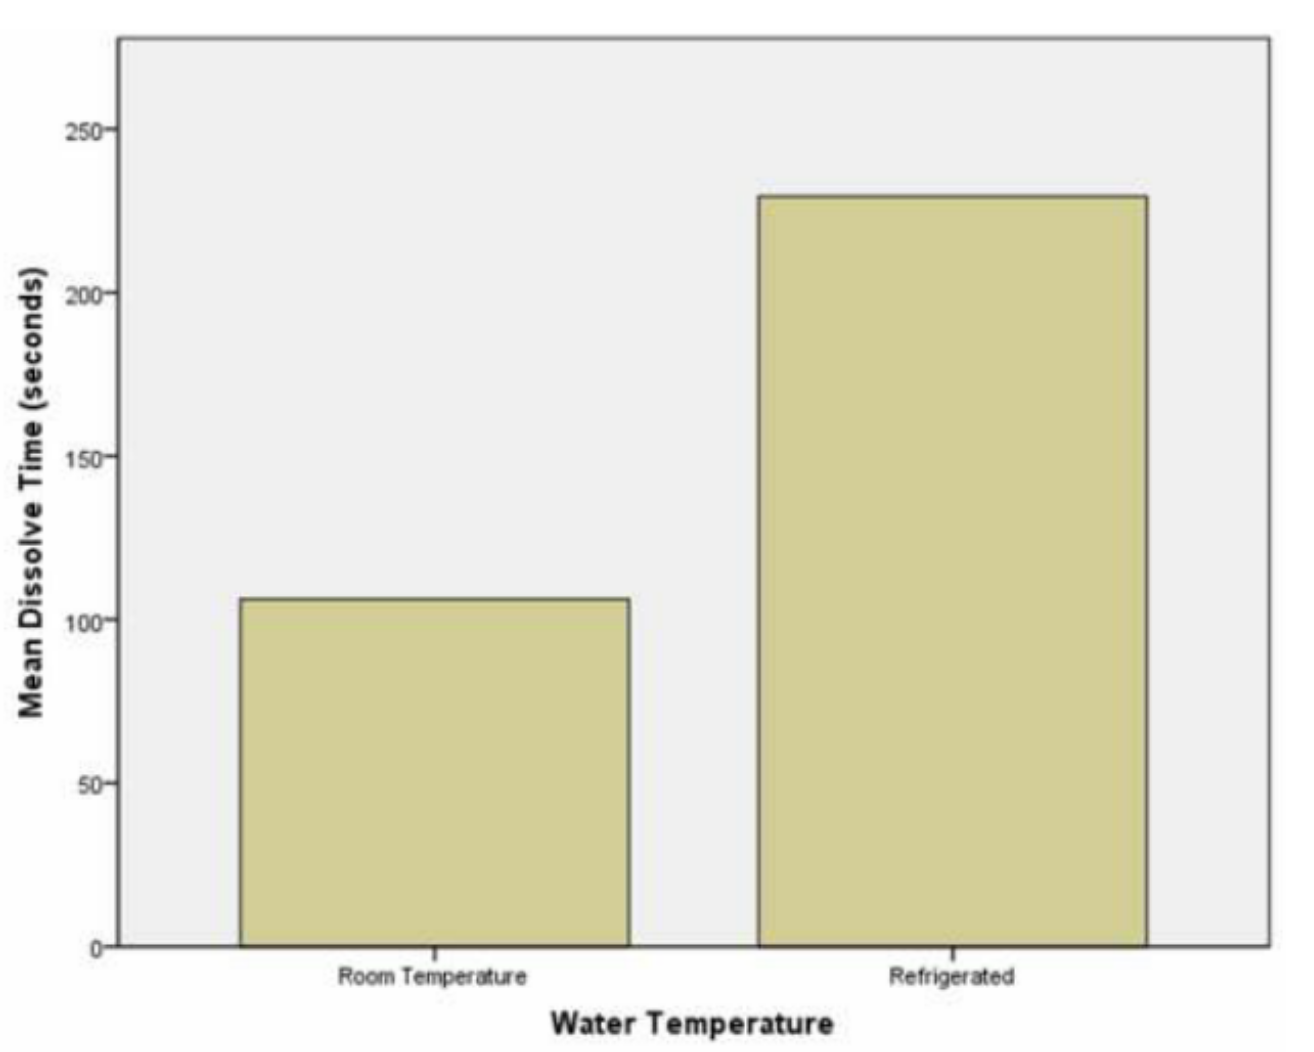
\includegraphics[width=0.7\linewidth]{ProjectImages/WrongBar} 

}

\caption{A graph from a student Project.}\label{fig:StudentsGraphsC}
\end{figure}

Make some notes about important things you learnt from this activity, to remember when creating your graphs for Task~2B.
\answerbox{4}

\section{Understanding correlations}\label{UnderstandCorrelations}

Answer the following questions, referring to Fig.~\ref{fig:GuessesCorr}.
The four correlation coefficients \(r\) are:

\begin{table}
\centering\begingroup\fontsize{10}{12}\selectfont

\begin{tabular}{cccc}
\toprule
\textbf{A}: $r = -0.95$\qquad\qquad & \textbf{B}: $r = 0.12$\qquad\qquad & \textbf{C}: $r = 0.75$\qquad\qquad & \textbf{D}: $r = 0.94$\\
\bottomrule
\end{tabular}
\endgroup{}
\end{table}

\begin{enumerate}
\def\labelenumi{\arabic{enumi}.}
\tightlist
\item
  For two plots, a correlation is not suitable.
  Which two?
  Explain your answer.
  \answerbox{2}
\item
  Determine which plot corresponds to which correlation coefficient.
  \answerbox{3}
\item
  Think of an example of two quantitative variables that might produce a plot with a \emph{direction} similar to \textbf{Plot 1}.
  \answerbox{3}
\item
  Think of an example of two quantitative variables that might produce a plot with a \emph{direction} similar to \textbf{Plot 2}.
  \answerbox{3}
\item
  Compute the values of \(R^2\) for each plot identified in \textbf{Part~1} of this question.
  \answerbox{4}
\end{enumerate}

\begin{figure}[hbtp]

{\centering 
\includegraphics[width=0.85\linewidth]{05-TW5-Tutorial_files/figure-latex/GuessesCorr-1} 

}

\caption{Six different scatterplots.}\label{fig:GuessesCorr}
\end{figure}

\section{Numerical summary for ruler-drop data}\label{PlanStudy4}

Your tutor will have information.

\section{Which summary measures to use}\label{WhichSummaryToUse}

A study of different orthoses (orthotic devices) in children with cerebral palsy (\citeproc{ref-data:Swinnen2017:orthoses}{Swinnen et al. 2017}) produced the demographic data of the participants.
\href{https://en.wikipedia.org/wiki/Gross_Motor_Function_Classification_System}{GMFCS} is the
`Gross Motor Function Classification System', which is a five-level classification system describing the gross motor function of people with cerebral palsy, based on self-initiated movement abilities.
(Higher classification numbers refer to less motor function.)

The data are shown in Fig.~\ref{fig:Orthoses}.

\begin{figure}[hbtp]

{\centering 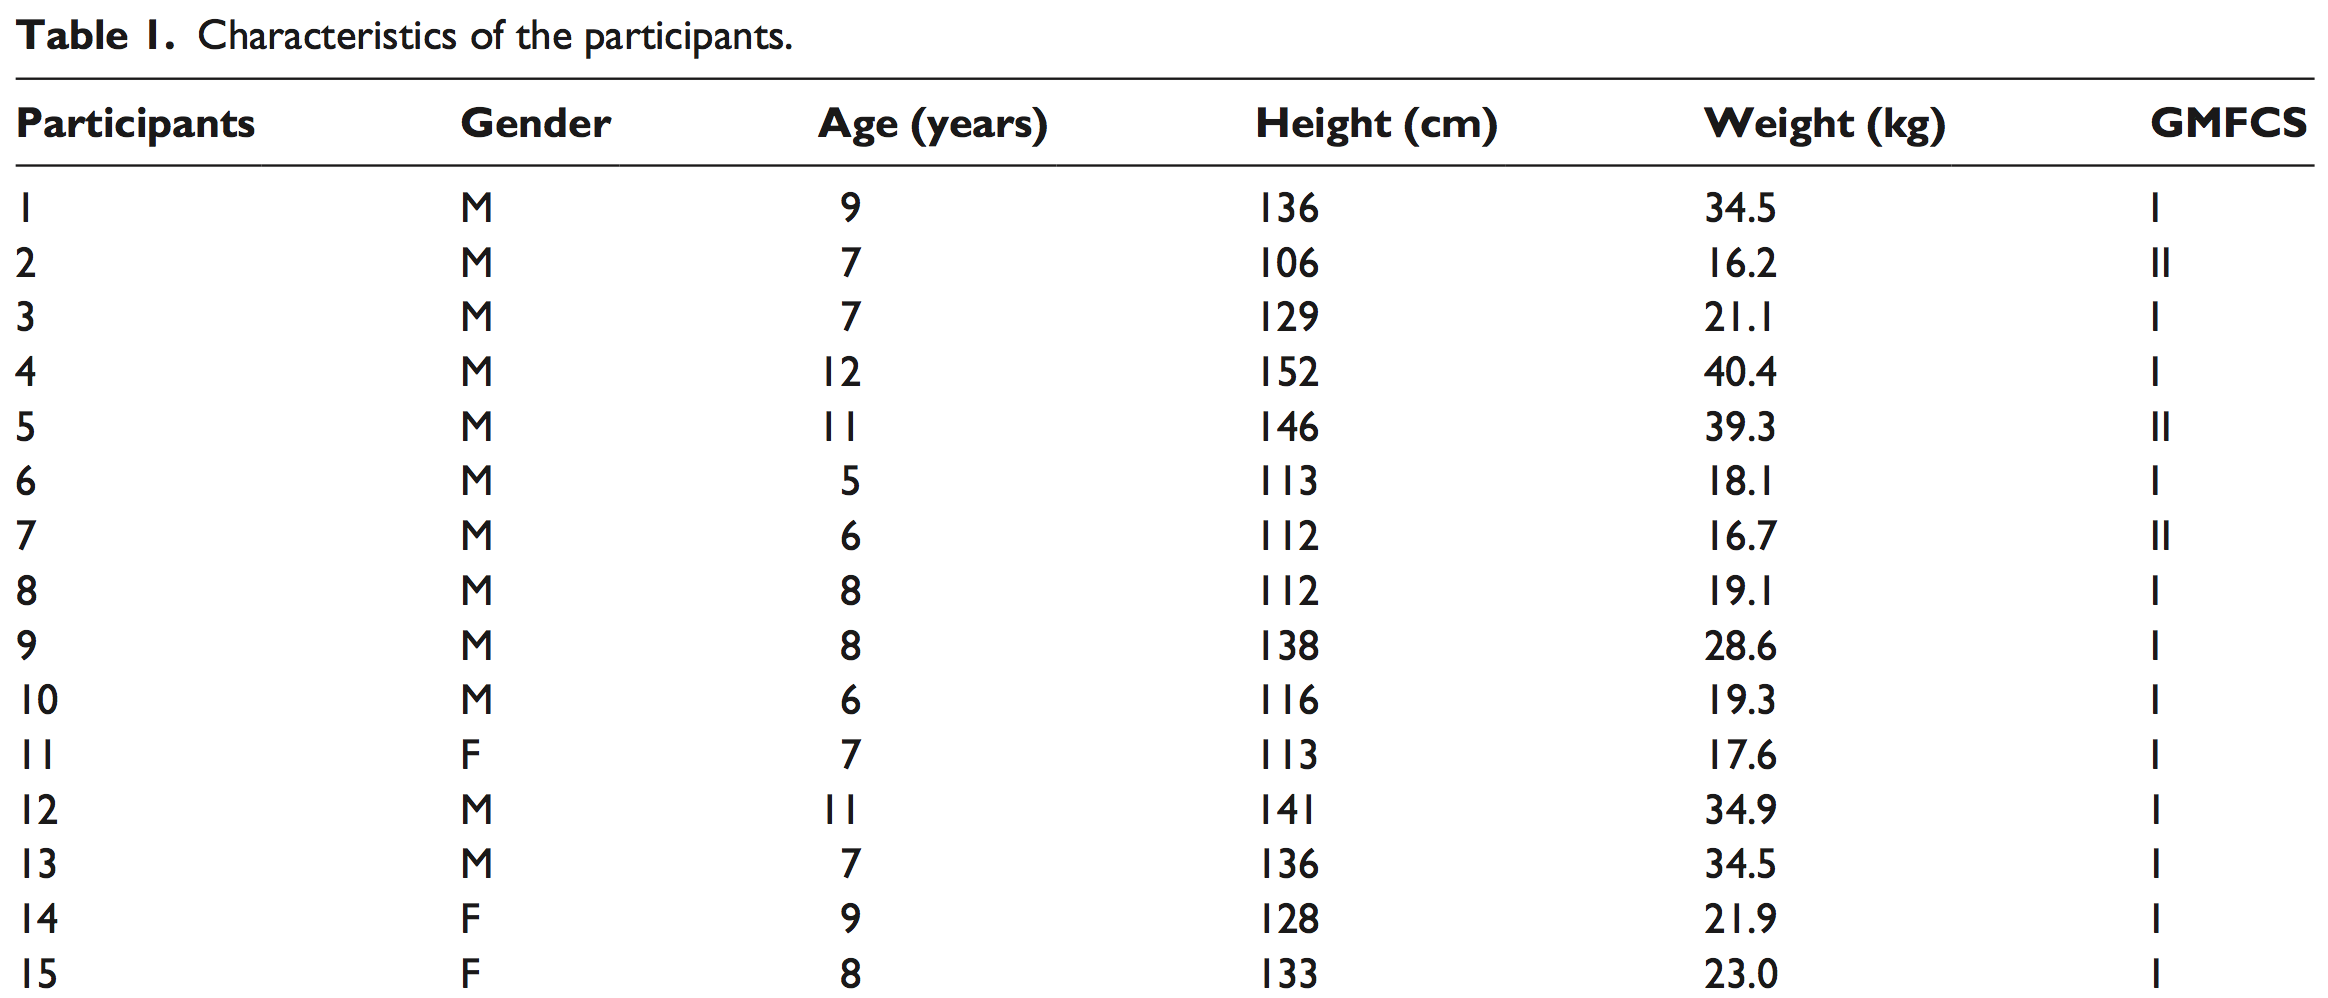
\includegraphics[width=0.95\linewidth]{ArticleImages/Swinnen-Table1-Cropped} 

}

\caption{The data collected from a study of orthoses (GMFCS: Gross Motor Function Classification System).}\label{fig:Orthoses}
\end{figure}

\begin{enumerate}
\def\labelenumi{\arabic{enumi}.}
\tightlist
\item
  How many quantitative \emph{continuous} variable(s) appear in the data set?
  Which are they?
  \answerbox{2}
\item
  How many qualitative \emph{ordinal} variable(s) appear in the data set?
  Which are they?
  \answerbox{2}
\item
  How many qualitative \emph{nominal} variable(s) appear in the data set?
  Which are they?
  \answerbox{2}
\end{enumerate}

\pagebreak

\begin{enumerate}
\def\labelenumi{\arabic{enumi}.}
\setcounter{enumi}{3}
\tightlist
\item
  What statistics could be used to \emph{numerically} summarise the variable \textbf{Age}?

  \begin{enumerate}
  \def\labelenumii{\alph{enumii}.}
  \tightlist
  \item
    Odds.
  \item
    Standard deviation.
  \item
    Percentage.
  \item
    Mean.
  \end{enumerate}
\item
  What statistics could be used to \emph{numerically} summarise the variable \textbf{Gender}?

  \begin{enumerate}
  \def\labelenumii{\alph{enumii}.}
  \tightlist
  \item
    Odds.
  \item
    Standard deviation.
  \item
    Percentage.
  \item
    Mean.
  \end{enumerate}
\item
  What statistics could be used to \emph{numerically} summarise the variable \textbf{GMFCS}?

  \begin{enumerate}
  \def\labelenumii{\alph{enumii}.}
  \tightlist
  \item
    Odds.
  \item
    Standard deviation.
  \item
    Percentage.
  \item
    Mean.
  \end{enumerate}
\item
  What graph could be used to \emph{graphically} summarise the variable \textbf{Age}?

  \begin{enumerate}
  \def\labelenumii{\alph{enumii}.}
  \tightlist
  \item
    Pie chart.
  \item
    Stem-and-leaf plot.
  \item
    Scatterplot.
  \item
    Boxplot.
  \item
    Bar chart.
  \item
    Histogram.
  \end{enumerate}
\item
  What graph could be used to \emph{graphically} summarise the variable \textbf{GMFCS}?

  \begin{enumerate}
  \def\labelenumii{\alph{enumii}.}
  \tightlist
  \item
    Pie chart.
  \item
    Stem-and-leaf plot.
  \item
    Scatterplot.
  \item
    Boxplot.
  \item
    Bar chart.
  \item
    Histogram.
  \end{enumerate}
\item
  What graph could be used to \emph{graphically} summarise the relationship between \textbf{Gender} and \textbf{Height}?

  \begin{enumerate}
  \def\labelenumii{\alph{enumii}.}
  \tightlist
  \item
    Pie chart.
  \item
    Side-by-side bar chart.
  \item
    Scatterplot.
  \item
    Boxplot.
  \item
    Bar chart.
  \item
    Histogram.
  \end{enumerate}
\item
  What graph could be used to \emph{graphically} summarise the relationship between \textbf{Gender} and \textbf{GMFCS}?

  \begin{enumerate}
  \def\labelenumii{\alph{enumii}.}
  \tightlist
  \item
    Pie chart.
  \item
    Side-by-side bar chart.
  \item
    Scatterplot.
  \item
    Boxplot.
  \item
    Bar chart.
  \item
    Histogram.
  \end{enumerate}
\end{enumerate}

\chapter{Teaching Week 6 tutorial}\label{Lecture6}

\begin{objectivesBox}{iconmonstr-target-4-240.png}

You will learn to:

\begin{itemize}
\tightlist
\item
  identify different methods for computing probabilities.
\item
  compute probabilities in simple situations.
\item
  understand the role of probability models for describing sampling variation.
\item
  describe sampling variation, and understand the role played by the sample size.
\item
  find the probability associated with a value on a normal distribution.
\item
  find the value associated with a probability in a normal distribution.
\end{itemize}

\end{objectivesBox}

\begin{assessmentBox}{iconmonstr-text-check-list-lined-240.png}

The Week~6 content is essential for:

\begin{itemize}
\tightlist
\item
  understanding the content that follows, \emph{all} of which relies on probability, understanding sampling variation, and using normal distributions;
\item
  \textbf{Quiz~3}, which includes questions about \emph{probability, sampling variation, and normal distributions}; and
\item
  the \textbf{Exam}, which will contain questions about \emph{probability, sampling variation, and normal distributions}.
\end{itemize}

\end{assessmentBox}

\begin{readBox}{iconmonstr-school-15-240.png}

You will learn and practice the content associated with these chapters of the \href{https://peterkdunn.github.io/SRM-Textbook/}{textbook}:

\begin{itemize}
\tightlist
\item
  \href{https://peterkdunn.github.io/SRM-Textbook/Probability.html}{Chapter~18 (Probability)}.
\item
  \href{https://peterkdunn.github.io/SRM-Textbook/SamplingVariation.html}{Chapter~19 (Sampling variation)}.
\item
  \href{https://peterkdunn.github.io/SRM-Textbook/SamplingDistributions.html}{Chapter~20 (Models and normal distributions)}.
\end{itemize}

\end{readBox}

\begin{tipBox}{iconmonstr-info-6-240.png}
You will need to access the normal distribution tables for this tutorial.
These Tables can be found in the textbook appendices, and in this document in
Appendices~\ref{ZTablesNEG} and~\ref{ZTablesPOS}.

\end{tipBox}

\pagebreak

\section{Quick revision}\label{QuickRevision-Tutorial6}

A new method for evaluating bridge loads (\citeproc{ref-obrien2018probabilistic}{O'Brien et al. 2018}) used a simulation to compare the new method to an existing method.
For the simulation, they modelled the gross vehicle mass (GVM) of trucks as having a normal distribution, with a mean of \(13\)~tonnes and a standard deviation of \(1.3\)~tonnes.

The
Isuzu F-Series trucks
are rated as having a GVM between \(10.7\) and \(26.0\)~tonnes (depending on the configuration; in 2024).

\begin{enumerate}
\def\labelenumi{\arabic{enumi}.}
\tightlist
\item
  What is the \(z\)-score for the lightest truck of \(10.7\)~tonnes? \tightlist
  \answerbox{2}
\item
  What is the \(z\)-score for the heaviest truck of \(26.0\)~tonnes?
  \answerbox{2}
\item
  What does a \emph{negative} \(z\)-score mean in this context?
  \answerbox{2}
\item
  \textbf{True} or \textbf{false}:
  A standard error measures the size of the difference between the \textbf{sample} proportion and the \textbf{population} proportion.
  Explain.
  \answerbox{2}
\end{enumerate}

\section{Class discussion}\label{TW6-Class-Discussion}

\begin{discussBox}{iconmonstr-speech-bubble-26-240.png}
\textbf{Discuss}: Outliers should \textbf{always} be removed from a dataset before analysis.

\end{discussBox}

\section{Normal distributions and IQs}\label{NormalIQs}

Standard IQs in current use (despite their flaws) are designed so that the IQ scores of the \emph{population} have a normal distribution with a mean of~\(100\), and a standard deviation of~\(15\).

\begin{enumerate}
\def\labelenumi{\arabic{enumi}.}
\tightlist
\item
  Draw a labelled picture of the normal distribution of the IQ scores in the \emph{population}.
  \answerbox{6}
\item
  For a person with an IQ of~\(130\), how many IQ points are they from the mean?
  \answerbox{2}
\item
  For a person with an IQ of~\(130\), how many \emph{standard deviations} is their IQ from the mean?
  \answerbox{2}
\item
  Draw a labelled picture of the normal distribution of the IQ scores, showing the proportion of the population with IQ scores of \(85\) and greater.
  \answerbox{5}
\item
  For a person with an IQ of~\(85\), how many IQ points are they from the mean?
  \answerbox{2}
\item
  For a person with an IQ of~\(85\), how many \emph{standard deviations} is their IQ from the mean?
  \answerbox{2}
\item
  Approximately, what proportion of the population has an IQ greater than~\(85\)?
  (Use the \(68\)--\(95\)--\(99.7\) rule.)
  \answerbox{2}
\end{enumerate}

\section{Normal distributions and heights}\label{NormalHeights}

In the \textit{National Nutrition Survey} (NNS) (conducted with the 1995~\emph{National Health Survey} (NHS)), trained nutritionists measured the heights of the respondents (\citeproc{ref-data:ABS1995:MeasureUp}{Australian Bureau of Statistics 1995}).

The values quoted are the population means~\(\mu\) and standard deviations~\(\sigma\) of the models used for heights.

\begin{enumerate}
\def\labelenumi{\arabic{enumi}.}
\tightlist
\item
  Take a wild guess: What percentage of your peers (people your age and gender) do you think would be \emph{shorter} than you?
  \_\_\_\_\_\_\_\_\%.
\item
  Write down your own height:
  \_\_\_\_\_\_\_\_cm.
\item
  From Fig.~\ref{fig:Ht}, write down the mean and standard deviation for people in your \emph{age group} and \emph{gender}.
  Using this information, compute the \(z\)-score for your height, relative to people in your age group and gender.
  Explain what this means.
  \answerbox{4}
\end{enumerate}

\begin{figure}[hbtp]

{\centering 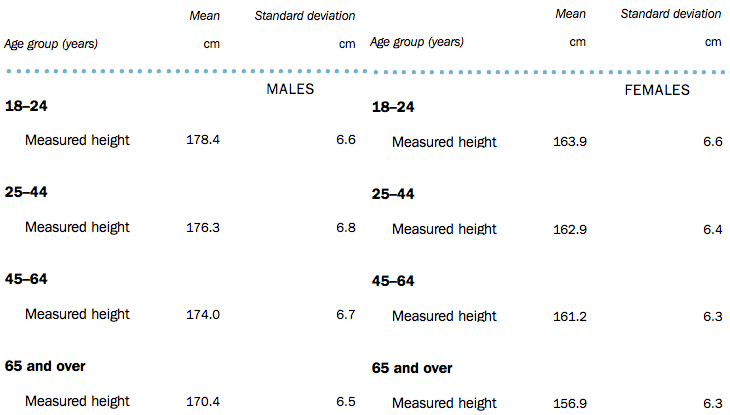
\includegraphics[width=0.85\linewidth]{ArticleImages/AustHtsSubWide-Measured-TOP} 

}

\caption{Part of the ABS report on heights of Australians.}\label{fig:Ht}
\end{figure}

\pagebreak

\begin{enumerate}
\def\labelenumi{\arabic{enumi}.}
\setcounter{enumi}{3}
\tightlist
\item
  Heights have an approximate normal (bell-shape) distribution, so the \(68\)--\(95\)--\(99.7\) rule applies.\\
  \textbf{Using the \(68\)--\(95\)--\(99.7\) rule}, \emph{roughly} estimate the percentage of people of your age and gender that are \emph{shorter} than you.
  (Hint: Draw a picture!)
  \answerbox{4}
\item
  Using \textbf{the normal distribution tables} in the Appendix, together with the information from \textbf{Fig.~\ref{fig:Ht}}, compute the percentage of people of your age and gender that are \emph{shorter} than you.
  \answerbox{3}
\end{enumerate}

For the remaining parts of this question, use data for \emph{females 18~and over} (where the mean is \(\mu = 161.4\,\text{cm}\), and the standard deviation is \(\sigma = 6.7\,\text{cm}\), drawn from Fig.~\ref{fig:Ht}.)

\begin{enumerate}
\def\labelenumi{\arabic{enumi}.}
\setcounter{enumi}{5}
\item
  Using the \(68\)--\(95\)--\(99.7\) rule, the middle \(95\)\% of \emph{females 18~and over} are within what height range?
  \answerbox{4}
\item
  Answer the following questions.

  \begin{enumerate}
  \def\labelenumii{\alph{enumii}.}
  \tightlist
  \item
    Compute the \emph{percentage} of females \(18\)~and over that are \emph{shorter} than \(171\,\text{cm}\).
    \answerbox{2}
  \item
    What are the \emph{odds} that a female \(18\)~and over is \emph{shorter} than \(171\,\text{cm}\)?
    \answerbox{2}
  \item
    Compute the \emph{percentage} of females \(18\)~and over that are \emph{taller} than \(171\,\text{cm}\)?
    \answerbox{2}
  \item
    What are the \emph{odds} that a female \(18\)~and over is \emph{taller} than \(171\,\text{cm}\)?
    \answerbox{2}
  \item
    Compute the \emph{percentage} of females \(18\)~and over that are \emph{between} \(170\) and \(180\,\text{cm}\)?
    \answerbox{2}
  \item
    What are the \emph{odds} that a female \(18\)~and over is \emph{between} \(170\) and \(180\,\text{cm}\)?
    \answerbox{2}
  \end{enumerate}
\item
  Approximately \(20\)\% of females \(18\)~and over are shorter than what height?
  \answerbox{2}
\end{enumerate}

\section{Probability}\label{Probability2}

For the following, indicate \emph{how} you could estimate the probability (classical; relative frequency; subjective) in these situations.
(\textbf{Note:} You are not asked to \emph{compute} the probability.)

\begin{enumerate}
\def\labelenumi{\arabic{enumi}.}
\tightlist
\item
  The probability that a given UniSC student lives in Nambour.\tightlist  
  \null
  \answerbox{1}
\item
  The probability that a given Nambour resident is a UniSC student.
  \null
  \answerbox{1}
\item
  The probability that Labor wins the next federal election.
  \null
  \answerbox{1}
\item
  The probability that you will throw a dart and hit the bullseye.
  \null
  \answerbox{1}
\item
  The probability that a roulette wheel spins a \(33\).
  \null
  \answerbox{1}
\end{enumerate}

Explain the difference between the meaning of the \textbf{first two} statements.
\answerbox{2}

\section{Random coin tosses}\label{RandomCardDraws}

\begin{wrapfigure}[5]{R}{.25\textwidth} % The first optional input is the number of lines allowed for the image to be placed in
  \centering%
  \vspace{-30pt}% This removes some white space
  
\includegraphics[width=.24\textwidth]{QRcodes/RandomOrgCoinToss.png}%
\end{wrapfigure}

In this activity, we see an example of a sampling distribution that can be described by a normal distribution.

Use
the website \url{https://www.random.org/coins/} (you can use the QR code to get there quickly)
to flip \textbf{ten} Australian one-dollar coins at random (see Fig.~\ref{fig:CoinTosser}).
Click \emph{Games} from the top, then \emph{Coin flipper}, then select the options to toss \(10\) coins, and use an Australian \$1 coin.)

Repeat this process numerous times (if you are in a class, each student can repeat the process numerous times so you get a large number of tosses), and complete
Table~\ref{tab:CoinDataTable}.

\begin{figure}[hbtp]

{\centering 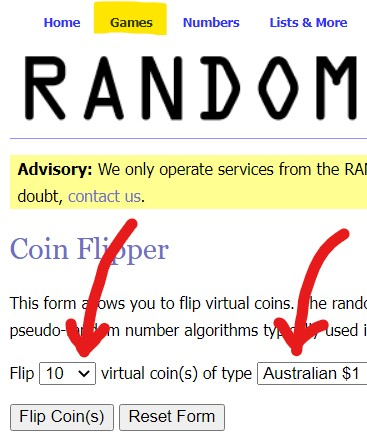
\includegraphics[width=0.35\linewidth]{images/CoinToss} 

}

\caption{Using the online random coin-tosser.}\label{fig:CoinTosser}
\end{figure}

\begin{table}
\centering
\caption{\label{tab:CoinDataTable}Tossing coins.}
\centering
\fontsize{10}{12}\selectfont
\begin{tabular}[t]{rr}
\toprule
\textbf{Proportion of heads in 10 tosses} & \textbf{How many times observed}\\
\midrule
0.0 (0 heads) & \\
\addlinespace\addlinespace\hline
0.1 (1 head)\phantom{0} & \\
\addlinespace\addlinespace\hline
0.2 (2 heads) & \\
\addlinespace\addlinespace\hline
0.3 (3 heads) & \\
\addlinespace\addlinespace\hline
0.4 (4 heads) & \\
\addlinespace\addlinespace\hline
0.5 (5 heads) & \\
\addlinespace\addlinespace\hline
0.6 (6 heads) & \\
\addlinespace\addlinespace\hline
0.7 (7 heads) & \\
\addlinespace\addlinespace\hline
0.8 (8 heads) & \\
\addlinespace\addlinespace\hline
0.9 (9 heads) & \\
\addlinespace\addlinespace\hline
1.0 (10 heads) & \\
\addlinespace\addlinespace\hline
\textbf{Number of tosses:} & \\
\bottomrule
\end{tabular}
\end{table}

\begin{enumerate}
\def\labelenumi{\arabic{enumi}.}
\tightlist
\item
  Use this data to create a histogram of the proportion of heads.
  Describe the histogram.
  \answerbox{4}
\item
  I also `tossed' \(10\)~coins, but repeated this random process \(400\)~times.
  My histogram is shown in Fig.~\ref{fig:HistCoinToss}.
  Describe the histogram.
  \answerbox{2}
\item
  Sketch the theoretical \emph{sampling distribution} of the sampling proportion.
  What does this sketch show you?
  \answerbox{4}
\item
  How would this \emph{sampling distribution} change if we looked the proportion of heads in \(50\)~tosses of a coin (rather than \(10\)~tosses)?
  \answerbox{2}
\end{enumerate}

\begin{figure}[hbtp]

{\centering 
\includegraphics[width=0.7\linewidth]{06-TW6-Tutorial_files/figure-latex/HistCoinToss-1} 

}

\caption{The histogram of the proportion of heads in $10$ tosses, for $400$ repetitions.}\label{fig:HistCoinToss}
\end{figure}

\section{\texorpdfstring{\textbf{Optional questions}}{Optional questions}}\label{OptionalTW6}

\begin{optionalBox}{iconmonstr-help-4-240.png}
These questions are \textbf{optional}; e.g., if you need more practice, or you are studying for the exam.
(Answers appear in Sect.~\ref{Lecture6Answers}.)

\end{optionalBox}

\subsection{\texorpdfstring{\textbf{(Optional)} Working with normal distributions}{(Optional) Working with normal distributions}}\label{NormalSOI}

\begin{videoSolutionBox}{iconmonstr-youtube-10-240.png}
This question has a video solution in the online book, so you can hear and see the solution.

\end{videoSolutionBox}

The Southern Oscillation Index (SOI) is a unitless\footnote{That is, it is not measured in kilograms or seconds etc. It is just a number; in fact, it is a bit like a \(z\)-score.} climatological measure that is easily computed, and has been shown to be related to the weather conditions in eastern Australia (\citeproc{ref-climate:stone:1992}{Stone and Auliciems 1992}; \citeproc{ref-mypapers:Dunn:bootstrap:2001}{Dunn 2001}).

The daily SOI has an approximate normal distribution, and is designed to have a mean of~\(0\) and a standard deviation of~\(10\).

\begin{enumerate}
\def\labelenumi{\arabic{enumi}.}
\tightlist
\item
  Draw a rough, labelled sketch of the theoretical distribution of the SOI values.
  \answerbox{4}
\item
  What is the probability that the daily SOI exceeds~\(20\)?
  \answerbox{2}
\item
  What are the \emph{odds} that the daily SOI exceeds~\(20\)?
  \answerbox{2}
\item
  What is the probability that the daily SOI is less than~\(-25\)?
  \answerbox{2}
\item
  What is the probability that the daily SOI is greater than~\(-12\)?
  \answerbox{2}
\item
  What is the probability that the daily SOI is between~\(-10\) and~\(20\)?
  \answerbox{2}
\item
  The SOI is \emph{less than} what value about~\(80\)\% of the time?
  \answerbox{2}
\item
  The SOI is \emph{greater} than what value about~\(35\)\% of the time?
  \answerbox{2}
\item
  What is the probability that the daily SOI exceeds~\(55\)?
  \answerbox{2}
\item
  The SOI is \emph{greater} than what value about~\(50\)\% of the time?
  \answerbox{2}
\end{enumerate}

\chapter{Teaching Week 7 tutorial}\label{Lecture7}

\begin{objectivesBox}{iconmonstr-target-4-240.png}

You will learn to:

\begin{itemize}
\tightlist
\item
  construct and understand confidence intervals for one proportion.
\item
  construct and understand confidence intervals for one mean.
\end{itemize}

\end{objectivesBox}

\begin{assessmentBox}{iconmonstr-text-check-list-lined-240.png}

The Week~7 content is essential for:

\begin{itemize}
\tightlist
\item
  \textbf{Task~2B}, which requires you to \emph{produce CIs for your data};
\item
  \textbf{Quiz~3}, which includes questions about \emph{understanding and producing CIs}; and
\item
  the \textbf{Exam}, which will contain questions about \emph{understanding and producing CIs}.
\end{itemize}

\end{assessmentBox}

\begin{readBox}{iconmonstr-school-15-240.png}

You will learn and practice the content associated with these chapters of the \href{https://peterkdunn.github.io/SRM-Textbook/}{textbook}:

\begin{itemize}
\tightlist
\item
  \href{https://peterkdunn.github.io/SRM-Textbook/IntroducingInference.html}{Chapter~21 (Introducing inference)}.
\item
  \href{https://peterkdunn.github.io/SRM-Textbook/CIOneProportion.html}{Chapter~22 (Confidence intervals: one proportions)}.
\item
  \href{https://peterkdunn.github.io/SRM-Textbook/OneMeanConfInterval.html}{Chapter~23 (Confidence intervals: one mean)}.
\item
  \href{https://peterkdunn.github.io/SRM-Textbook/AboutCIs.html}{Chapter~24 (More details about CIs)}.
\end{itemize}

\end{readBox}

\pagebreak

\section{Quick revision}\label{QuickRevision-Tutorial7}

\begin{enumerate}
\def\labelenumi{\arabic{enumi}.}
\tightlist
\item
  \textbf{True} or \textbf{false}: A \emph{confidence interval} is used to find an interval that probably (but not certainly) contains the \emph{sample} value. \tightlist
  \answerbox{1}
\item
  \textbf{True} or \textbf{false}: All \emph{confidence interval} are \(95\)\% confidence intervals.
  \answerbox{1}
\item
  \textbf{True} or \textbf{false}: A \emph{standard error} is calculated from population data, but a \emph{standard deviation} is calculated from sample data.
  \answerbox{1}
\item
  \textbf{True} or \textbf{false}: CIs answers estimation-type RQs.
  \answerbox{1}
\item
  \textbf{True} or \textbf{false}: A 95\% confidence interval will contain approximately 95\% of the observations.
  \answerbox{1}
\end{enumerate}

\section{Class discussion}\label{TW7-Class-Discussion}

\begin{discussBox}{iconmonstr-speech-bubble-26-240.png}
\textbf{Discuss}: If we have \emph{greater} confidence in our answer, we would expect to have a \emph{smaller} range of values to choose from (i.e., a narrower CI).

\end{discussBox}

\section{Concepts}\label{ConceptsMatches}

Claire and Jake were wondering about the mean number of matches in a box.
The boxes contain this statement:

\begin{quote}
An average of \(45\) matches per box.
\end{quote}

They purchased a carton containing \(25\)~boxes of matches, and Jake counted the number of matches in \emph{one} of those \(25\)~boxes.
There was \(44\)~matches.

``Oh wow. Just wow\ldots{}'' said Jake.
``They lie. There's only \(44\)~matches in this box.''

\begin{enumerate}
\def\labelenumi{\arabic{enumi}.}
\item
  Identify the two statistical concepts that Jake is confusing.
  How would you clarify the confusion?\tightlist
  \answerbox{2}
\item
  Then, Jake and Claire counted the number of matches in \emph{each} of the twenty-five boxes.
  Claire found that the mean number of matches per box was \(44.9\)~matches, and the standard deviation was \(0.124\).

  Jake says, ``A mean of \(44.9\)~matches per box?
  You can't have \(0.9\) of a match!
  That's dumb.''
  How would you respond?
  \answerbox{2}
\item
  ``The claim is \(45\)~matches per box on average, but the mean really is \(44.9\)!'' said Jake.
  ``They're liars! Liar, liar, pants on\ldots{}''

  Identify the two statistical concepts that Jake is confusing.
  How would you clarify the confusion?
  \answerbox{2}
\item
  What two broad reasons could explain why the sample mean is \emph{not} \(45\)?
  \answerbox{2}
\item
  Claire says, ``The mean won't be \emph{exactly} \(45\) in every sample of \(25\) boxes!
  Let's work out the confidence interval.''

  Why does Claire think a CI is needed?
  What will it tell them?
  \answerbox{2}
\item
  Would the standard deviation of the number of matches in a box be more likely to be \(0.04\)~matches, \(0.4\)~matches or \(4\)~matches?
  Explain.
  \answerbox{2}
\item
  Compute an approximate \(95\)\% confidence interval for the mean for Claire's sample.
  \answerbox{2}
\item
  ``Aha---I told you so!
  They \emph{are} absolutely lying!
  Your confidence interval doesn't even include their mean of \(45\)!'' said Jake.
  ``The manufacturer \emph{must} be lying!
  I'm calling my lawyer!''

  Is Jake correct that the manufacturer \emph{must} be lying?
  Why or why not?
  What does the CI \emph{mean}?
  \answerbox{2}
\item
  In this scenario, what does~\(\bar{x}\) represent?
  What is the \emph{value} of~\(\bar{x}\)?
  \answerbox{2}
\item
  In this scenario, what does~\(\mu\) represent?
  What is the \emph{value} of~\(\mu\)?
  \answerbox{2}
\end{enumerate}

\section{Standard error formulas}\label{SEproportions}

Two formulas for the \textbf{standard error} are:\\
\[
  \text{s.e.}(\hat{p}) = \sqrt{\frac{\hat{p} \times (1 - \hat{p})}{n}}
  \qquad
  \text{and}
  \qquad
  \text{s.e.}(\bar{x}) = \frac{s}{\sqrt{n}}.
\]

\begin{enumerate}
\def\labelenumi{\arabic{enumi}.}
\tightlist
\item
  When should each formula be used?
  \answerbox{1}
\item
  What does~\(\hat{p}\) represent?
  \answerbox{1}
\item
  What does~\(n\) represent?
  \answerbox{1}
\item
  What does~\(s\) represent?
  \answerbox{1}
\item
  What does ``\(\text{s.e.}\)'' represent?
  \answerbox{1}
\end{enumerate}

\section{CIs for one proportion}\label{CIPropBVM}

Endotracheal intubation (ETI) is a method for maintaining an open airway or as a method for administering certain drugs for ill patients.
ETI is widely used for airway management of children in the out-of-hospital setting, but for many years little evidence was available on the effect of using ETI.
The BVM (`ball valve mask') method is also used.

Gausche et al. (\citeproc{ref-data:Gausche200:Endotracheal}{2000}) examined the use of ETI for airway management of children in the out-of-hospital setting.

\begin{figure}[hbtp]

{\centering 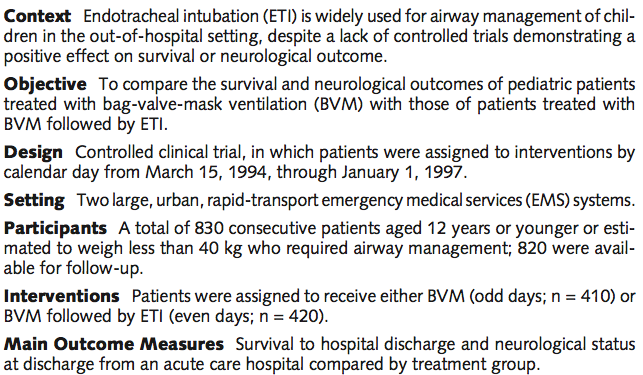
\includegraphics[width=0.7\linewidth]{ArticleImages/Gausche2000-PartialAbstract} 

}

\caption{Part of the Abstract from Gausche et al. (2000).}\label{fig:Gausche2000Abstract}
\end{figure}

\begin{enumerate}
\def\labelenumi{\arabic{enumi}.}
\tightlist
\item
  For the \textbf{BVM sample}, \(123\) out of the \(404\)~patients survived.
  For those receiving BVM, compute the sample \emph{odds} of a patient who survived.
  \answerbox{2}
\item
  For the \textbf{BVM sample}, \(123\) out of the \(404\)~patients survived.
  For those receiving BVM, compute an estimate of the population \emph{proportion} of patients who survive.
  \answerbox{2}
\item
  Explain the difference between the meaning of the two above calculations.
  \answerbox{2}
\item
  In another sample of \(404\)~patients who received the BVM treatment, would we expect to find \emph{exactly} \(123\) surviving?
  Why or why not?
  \answerbox{2}
\item
  Compute the \emph{standard error} of~\(\hat{p}\), which indicates the sampling variability in the estimate of~\(p\).
  Explain what is meant by the term `sampling variation' in this context.
  \answerbox{2}
\item
  Every time a new sample is chosen, the sample will likely yield a different value for~\(\hat{p}\).
  Sketch the distribution that shows how much the value of~\(\hat{p}\) is likely to change from one sample to the next.
  \answerbox{4}
\item
  Compute an approximate \(95\)\% confidence interval for the population proportion based on the sample proportion.
  \answerbox{4}
\item
  Write a sentence communicating this confidence interval.
  \answerbox{3}
\item
  If the researchers wished to estimate the true survival proportion to within give-or-take \(0.01\) with \(95\)\% confidence, would the sample size need to be \emph{larger} or \emph{smaller}?
  \answerbox{2}
\item
  Confirm that the conditions necessary for this calculation to be statistically valid are met.
  \answerbox{2}
\end{enumerate}

\section{CIs for one mean}\label{CIPizzas}

In 2011, \emph{Eagle Boys Pizza} ran a campaign that claimed (among many other claims) that Eagle Boys pizzas were `Real size \(12\)-inch large pizzas' in an effort to out-market \emph{Dominos Pizza}.

Eagle Boy's made the data behind the campaign publicly available (\citeproc{ref-mypapers:Dunn:PizzaSize}{Dunn 2012}).
A summary of the diameters of a sample of \(125\) of Eagle Boys' large pizzas is shown in Fig.~\ref{fig:PizzaCIjamovi}.

\begin{figure}[hbtp]

{\centering 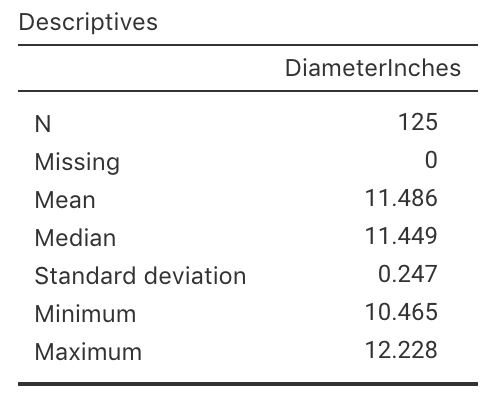
\includegraphics[width=0.42\linewidth]{SoftwareImages/PizzaDiameters-jamovi} 

}

\caption{Summary statistics for the diameter of Eagle Boys' large pizzas.}\label{fig:PizzaCIjamovi}
\end{figure}

\begin{enumerate}
\def\labelenumi{\arabic{enumi}.}
\item
  What do~\(\mu\) and~\(\bar{x}\) represent in this context? \tightlist 
  \answerbox{2}
\item
  Write down the \emph{values} of~\(\mu\) and~\(\bar{x}\).
  \answerbox{2}
\item
  Write down the \emph{values} of~\(\sigma\) and~\(s\).
  \answerbox{2}
\item
  Compute the value of the standard error of the mean.
  \answerbox{2}
\item
  Explain the difference in \emph{meaning} between \(s\) and \(\text{s.e.}(\bar{x})\) here.
  \answerbox{2}
\item
  If someone else takes a sample of \(125\)~Eagle Boys pizzas, will the sample mean be \(11.486\)~inches again (as it is in this sample)?
  Why or why not?
  \answerbox{2}
\item
  Draw a picture of the approximate sampling distribution for~\(\bar{x}\).
  \answerbox{4}
\item
  Compute an approximate \(95\)\% confidence interval for the mean pizza diameter.
  \answerbox{4}
\item
  Write a statement that communicates your \(95\)\%~CI for the mean pizza diameter.
  \answerbox{4}
\item
  What are the \textbf{statistical} validity conditions?
  \answerbox{2}
\item
  Which of these conditions must we \textbf{assume} are true for this CI to be \textbf{statistically} valid?
  How does Fig.~\ref{fig:PizzaHistoCI} help, if at all?
  Explain.

  \begin{itemize}
  \tightlist
  \item
    The sample size is greater than about~\(25\).
  \item
    The population has a normal distribution.
  \item
    The population standard deviation is known.
  \item
    The sample has a normal distribution.
  \end{itemize}
\end{enumerate}

\answerbox{2}

\begin{figure}[hbtp]

{\centering 
\includegraphics[width=0.65\linewidth]{07-TW7-Tutorial_files/figure-latex/PizzaHistoCI-1} 

}

\caption{Histogram for the diameter of Eagle Boys' large pizzas. The cross is the claimed diameter of 12 inches.}\label{fig:PizzaHistoCI}
\end{figure}

\begin{enumerate}
\def\labelenumi{\arabic{enumi}.}
\setcounter{enumi}{11}
\tightlist
\item
  Do you think that, on average, the pizzas do have a mean diameter of \(12\)~inches in the population, as Eagle Boy's claim?
  Explain.
  \answerbox{2}
\end{enumerate}

\section{\texorpdfstring{\textbf{Optional drills}: Computational exercises}{Optional drills: Computational exercises}}\label{Chapter6Drills}

\emph{(Answers appear in Sect. \ref{Lecture6Answers})}

\begin{drillBox}{iconmonstr-pencil-9-240.png}
These \emph{optional} \textbf{Drill} exercises (repeated practice) give you practice at getting computations correct, and using your calculator.
These drill questions are more about practising the underlying \emph{mathematics} rather than the \emph{statistics}.
If you need help, please \textbf{ask}.

\end{drillBox}

The \emph{standard error} for a sample proportion is calculated as\\
\[
   \text{s.e.}(\hat{p}) = \sqrt{\frac{\hat{p} \times (1 - \hat{p})}{n}}.
\]
The standard error quantifies how much the sample proportion is likely to vary from sample to sample.

Compute the standard error in these situations:

\begin{enumerate}
\def\labelenumi{\arabic{enumi}.}
\tightlist
\item
  When \(n = 25\) and \(\hat{p} = 0.70\).
  \answerbox{3}
\item
  When \(n = 100\) and \(\hat{p} = 0.25\).
  \answerbox{3}
\item
  When \(n = 32\) and \(\hat{p} = 0.42\).
  \answerbox{3}
\item
  When \(n = 53\) and \(\hat{p} = 0.814\).
  \answerbox{3}
\end{enumerate}

Will the CIs be statistically valid in the above situations?
\answerbox{3}

\chapter{Teaching Week 8 tutorial}\label{Lecture8}

\begin{objectivesBox}{iconmonstr-target-4-240.png}

You will learn to:

\begin{itemize}
\tightlist
\item
  explain and use the decision-making process.
\item
  conduct and understand hypothesis tests for one proportion.
\item
  conduct and understand hypothesis tests for one mean.
\item
  explain and understand \(P\)-values.
\end{itemize}

\end{objectivesBox}

\begin{assessmentBox}{iconmonstr-text-check-list-lined-240.png}

The Week~8 content is essential for:

\begin{itemize}
\tightlist
\item
  \textbf{Task~2B}, which requires you to \emph{conduct a hypothesis test for your data};
\item
  \textbf{Quiz~3}, which includes questions about \emph{understanding and conducting hypothesis tests}; and
\item
  the \textbf{Exam}, which will contain questions about \emph{understanding and conducting hypothesis tests}.
\end{itemize}

\end{assessmentBox}

\begin{readBox}{iconmonstr-school-15-240.png}

You will learn and practice the content associated with these chapters of the \href{https://peterkdunn.github.io/SRM-Textbook/}{textbook}:

\begin{itemize}
\tightlist
\item
  \href{https://peterkdunn.github.io/SRM-Textbook/MakingDecisions.html}{Chapter~25 (Making decisions)}.
\item
  \href{https://peterkdunn.github.io/SRM-Textbook/TestOneProportion.html}{Chapter~26 (Hypothesis tests: one proportion)}.
\item
  \href{https://peterkdunn.github.io/SRM-Textbook/TestOneMean.html}{Chapter~27 (Hypothesis tests: one mean)}.
\item
  \href{https://peterkdunn.github.io/SRM-Textbook/MoreAboutTests.html}{Chapter~28 (More details about hypothesis testing)}.
\end{itemize}

\end{readBox}

\pagebreak

\section{Quick revision}\label{QuickRevision-Tutorial8}

\begin{enumerate}
\def\labelenumi{\arabic{enumi}.}
\tightlist
\item
  \textbf{True} or \textbf{false}: Hypothesis tests are used to \emph{prove} or \emph{disprove} the null hypothesis. \tightlist
  \answerbox{1}
\item
  \textbf{True} or \textbf{false}: Hypotheses are \emph{always} written in terms of population parameters.
  \answerbox{1}
\item
  \textbf{True} or \textbf{false}: Alternative hypotheses may be one- or two-tailed, depending on the \textbf{data}.
  \answerbox{1}
\item
  \textbf{True} or \textbf{false}: Hypotheses should be constructed without any knowledge of the data.
  \answerbox{1}
\item
  \textbf{True} or \textbf{false}:
  The sampling distribution shows how the values of the sample statistic are likely to vary from sample to sample (when the null hypothesis is true).
  \answerbox{1}
\end{enumerate}

\section{Class discussion}\label{TW8-Class-Discussion}

\begin{discussBox}{iconmonstr-speech-bubble-26-240.png}
\textbf{Discuss}: Confidence intervals are more informative than \(P\)-values.

\end{discussBox}

\section{The decision-making process: dice}\label{DecisionMakingProcessDice}

Fill in the blanks in this piece of text,
using words and phrases from Table~\ref{tab:Words3Table}.

\begin{quote}
\begin{itemize}
\tightlist
\item
  Suppose I wish to see if a six-sided die is fair.\\
\item
  I could assess this in many ways.
  For example, my \_\_\_\_\_\_\_\_\_\_ could be that the proportion of odd numbers is \(0.5\).
  This value is a \_\_\_\_\_\_\_\_\_\_.\\
\item
  The \_\_\_\_\_\_\_\_\_\_ would be ``the proportion of odd numbers in the sample''.\\
\item
  We would \_\_\_\_\_\_\_\_\_\_ that the value of the statistic would be near \(0.5\) (but maybe not exactly \(0.5\)).\\
\item
  If I roll the die \(100\) times and observe \textbf{53} odd numbers, this seems \_\_\_\_\_\_\_\_\_\_ with what I would expect if the assumption was true.\\
\item
  If I roll the die \(100\) times and observe \textbf{zero} odd numbers, this seems \_\_\_\_\_\_\_\_\_\_ with what I would expect if the assumption was true.
\end{itemize}
\end{quote}

\begin{table}
\centering
\caption{\label{tab:Words3Table}Words and phrases to insert.}
\centering
\fontsize{10}{12}\selectfont
\begin{tabular}[t]{ccc}
\toprule
assumption & consistent & inconsistent\\
statistic & expect & parameter\\
\bottomrule
\end{tabular}
\end{table}

\section{Test for one proportion}\label{HTOneProportionA}

According to
Statistica.com,
\(30\)\% of individuals in Sweden wore contact lenses in 2020 (the highest percentage in Europe).

Suppose a group of \(35\)~Swedish computer programmers at a large company includes \(12\)~that wear contact lenses.
Is there evidence in this sample that a \emph{greater} proportion of Swedish programmers wear contact lenses at this company, compared to the general Swedish population?

\begin{enumerate}
\def\labelenumi{\arabic{enumi}.}
\tightlist
\item
  Write the hypotheses for conducting the appropriate hypothesis test.
  \answerbox{2}
\item
  Compute the value of the appropriate sample statistic.
  \answerbox{2}
\item
  Compute the value of the appropriate standard error of the statistic.
  What does this value \emph{mean}?
  \answerbox{2}
\item
  Compute the value of the appropriate test statistic.
  \answerbox{3}
\item
  Write a conclusion (including a CI).
  \answerbox{5}
\item
  What assumptions are needed for this test to be statistically valid, and externally valid?
  \answerbox{2}
\end{enumerate}

\section{Tests for one mean}\label{HTOneMean-A}

In 2011, \emph{Eagle Boys Pizza} ran a campaign that claimed that Eagle Boys' pizzas were `Real size \(12\)-inch large pizzas' (\citeproc{ref-mypapers:Dunn:PizzaSize}{Dunn 2012}).
Eagle Boys made the data from the campaign publicly available.

A summary of the diameters of a sample of \(125\) of their large pizzas is shown in Fig.~\ref{fig:PizzaSoftwareHTjamovi}.
We would like to test the company's claim, and ask the RQ:

\begin{quote}
For Eagle Boys' pizzas, is mean diameter actually \(12\) inches, or not?
\end{quote}

\begin{figure}[hbtp]

{\centering 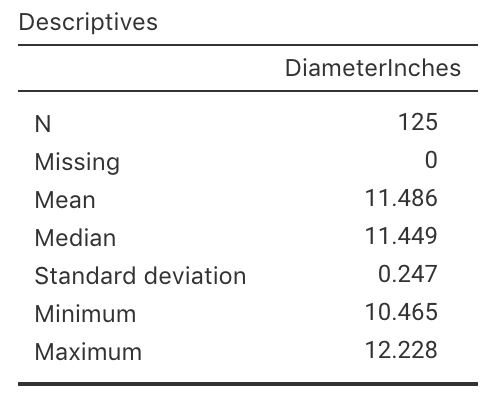
\includegraphics[width=0.4\linewidth]{SoftwareImages/PizzaDiameters-jamovi} 

}

\caption{Summary statistics for the diameter of Eagle Boys' large pizzas.}\label{fig:PizzaSoftwareHTjamovi}
\end{figure}

\begin{enumerate}
\def\labelenumi{\arabic{enumi}.}
\tightlist
\item
  What is the \textbf{parameter} of interest?
  \answerbox{1}
\item
  Write down the values of~\(\bar{x}\) and~\(s\).
  \answerbox{2}
\item
  Determine the value of the standard error of the mean.
  \answerbox{1}
\item
  Explain the difference in meaning between~\(s\) and \(\text{s.e.}(\bar{x})\) in this context.
  \answerbox{2}
\item
  Write the hypotheses to test if the mean pizza diameter is \(12\)~inches.
  \answerbox{2}
\item
  Is the alternative hypothesis one- or two-tailed? Why?
  \answerbox{2}
\item
  Draw the normal distribution that shows how the \emph{sample mean pizza diameter} would vary by chance, \emph{even if} the population mean diameter was \(12\)~inches.
  \answerbox{4}
\item
  Compute the \(t\)-score for testing the hypotheses.
  \answerbox{2}
\item
  What is the approximate \(P\)-value using the \(68\)--\(95\)--\(99.7\) rule?
  \answerbox{2}
\item
  Write a conclusion.
  (The CI was found in the \hyperref[CIPizzas]{Teaching Week~7 tutorial}.)
  \answerbox{3}
\item
  Is it reasonable to assume the \emph{statistical} validity conditions are satisfied?
  How does Fig. \ref{fig:PizzaHistoHT} help, if at all?
  \answerbox{2}
\item
  Do you think that the pizzas do have a mean diameter of \(12\)~inches in the population, as Eagle Boys' claim?
  Explain.
  \answerbox{2}
\end{enumerate}

\begin{figure}[hbtp]

{\centering 
\includegraphics[width=0.7\linewidth]{08-TW8-Tutorial_files/figure-latex/PizzaHistoHT-1} 

}

\caption{Histogram for the diameter of Eagle Boys' large pizzas. The cross represents the claimed diameter of $12$ inches.}\label{fig:PizzaHistoHT}
\end{figure}

\section{\texorpdfstring{Approximate \(P\)-values}{Approximate P-values}}\label{PValues}

Assuming the tests are statistically valid, what is the approximate \(P\)-value for a \emph{two}-tailed \(t\)-test if:

\begin{cols}

\begin{col}{0.2\textwidth}

\begin{enumerate}
\def\labelenumi{\arabic{enumi}.}
\tightlist
\item
  \(t = -2.14\).
\item
  \(t = 1.90\).
\item
  \(t = 3.15\).
\end{enumerate}

\end{col}

\begin{col}{0.05\textwidth}
~


\end{col}

\begin{col}{0.2\textwidth}

\begin{enumerate}
\def\labelenumi{\arabic{enumi}.}
\setcounter{enumi}{3}
\tightlist
\item
  \(t = -1.20\).
\item
  \(t = -1.59\).
\item
  \(t = 6.71\).
\end{enumerate}

\end{col}

\end{cols}

(\textbf{Hint}: Use the \(68\)--\(95\)--\(99.7\) rule.)
\answerbox{5}

How would your answers change if these \(t\)-scores came from a \emph{one-tailed} test?
\answerbox{2}

\section{Writing conclusions}\label{HtestWritingConclusions}

University~A advertises that \(40\)\% of its students are using AI daily.
To assess the claim, the student union takes a sample of \(78\)~students, and finds~\(29\) are using AI daily.
Using software, the \(z\)-score was \(z = -0.515\).

\begin{enumerate}
\def\labelenumi{\arabic{enumi}.}
\item
  Each of these alternative hypotheses is \textbf{incorrect}.
  Explain the main reason why.
  Then, write the \textbf{correct} alternative hypothesis.

  \begin{enumerate}
  \def\labelenumii{\alph{enumii}.}
  \tightlist
  \item
    \(H_1\): The proportion of students using AI daily is significantly lower than~\(0.40\).
  \item
    \(H_1 \ne 0.40\).
  \item
    \(H_1\): \(p < 0.40\), where~\(p\) is the population proportion of students using AI daily.
  \item
    \(H_1\): The number of students using AI daily is not equal to the university's claim.
    \answerbox{3}
  \end{enumerate}
\item
  Estimate the \(P\)-value.
  \answerbox{2}
\end{enumerate}

\pagebreak

\begin{enumerate}
\def\labelenumi{\arabic{enumi}.}
\setcounter{enumi}{2}
\item
  Each of these conclusions are \textbf{incorrect}.
  Explain the main reason why.
  Then, write the \textbf{correct} conclusion.

  \begin{enumerate}
  \def\labelenumii{\alph{enumii}.}
  \tightlist
  \item
    There is strong evidence that the proportion of students using AI daily is~\(0.40\).
  \item
    There is no evidence of a large difference between the population proportion of students using AI daily and the claimed proportion.
  \item
    The sample proportion is~\(0.40\).
    \answerbox{3}
  \end{enumerate}
\end{enumerate}

University~B makes the same claim.
To assess the claim, the student union takes a sample of \(66\)~students and finds~\(35\) are using AI daily.
Using software, the \(z\)-score was \(z = 2.12\).

\begin{enumerate}
\def\labelenumi{\arabic{enumi}.}
\setcounter{enumi}{3}
\item
  Estimate the \(P\)-value.
  \answerbox{2}
\item
  Each of these conclusions are \textbf{incorrect}.
  Explain the main reason why.
  Then, write the \textbf{correct} conclusion.

  \begin{enumerate}
  \def\labelenumii{\alph{enumii}.}
  \tightlist
  \item
    There is evidence of a significant difference between the population proportion of students using AI daily and the claim.
  \item
    There is no evidence that the claimed proportion is~\(0.40\).
  \item
    The claimed proportion is not~\(0.40\).
    \answerbox{3}
  \end{enumerate}
\end{enumerate}

\section{\texorpdfstring{\textbf{Optional questions}}{Optional questions}}\label{OptionalTW8}

\begin{optionalBox}{iconmonstr-help-4-240.png}
These questions are \textbf{optional}; e.g., if you need more practice, or you are studying for the exam.
(Answers appear in Sect.~\ref{Lecture6Answers}.)

\end{optionalBox}

\subsection{\texorpdfstring{\textbf{(Optional)} The decision-making process}{(Optional) The decision-making process}}\label{DecisionMakingProcess}

Fill in the blanks in this piece of text, using words and phrases from Table~\ref{tab:Words1Table}.

\begin{quote}
\begin{itemize}
\tightlist
\item
  The decision-making process begins with making an assumption about the population \_\_\_\_\_\_\_\_\_\_.\\
\item
  This means we know what to \_\_\_\_\_\_\_\_\_\_ from the sample \_\_\_\_\_\_\_\_\_\_.\\
\item
  We never know exactly what value of the statistic we will see in the sample, because of \_\_\_\_\_\_\_\_\_\_.\\
\item
  But we can have some of idea of what values are reasonable to expect.\\
\item
  Then we take the \_\_\_\_\_\_\_\_\_\_ (that is, we make the observations).\\
\item
  Then we \_\_\_\_\_\_\_\_\_\_ what the sample statistic that we observed\ldots{} to the sample statistic we expected.\\
\item
  If what we observe is inconsistent with what was expected, then the the assumption is \_\_\_\_\_\_\_\_\_\_ true.\\
\item
  However, if what we observe is \_\_\_\_\_\_\_\_\_\_ with what was expected, then the the assumption is \_\_\_\_\_\_\_\_\_\_ true.
\end{itemize}
\end{quote}

\begin{table}
\centering
\caption{\label{tab:Words1Table}Words and phrases to insert.}
\centering
\fontsize{10}{12}\selectfont
\begin{tabular}[t]{ccccc}
\toprule
compare & probably & expect & sampling variation & consistent\\
unlikely to be & sample & parameter & statistic & \\
\bottomrule
\end{tabular}
\end{table}

\chapter{Teaching Week 9 tutorial}\label{Lecture9}

\begin{objectivesBox}{iconmonstr-target-4-240.png}

You will learn to:

\begin{itemize}
\tightlist
\item
  construct CIs and conduct hypothesis tests for the mean difference in paired situations.
\item
  construct CIs and conduct hypothesis tests for comparing two independent means.
\end{itemize}

\end{objectivesBox}

\begin{assessmentBox}{iconmonstr-text-check-list-lined-240.png}

The Week~9 content is essential for:

\begin{itemize}
\tightlist
\item
  \textbf{Task~2B}, which requires you to \emph{produce CIs and conduct a hypothesis test for your data};
\item
  \textbf{Quiz~4}, which includes questions about \emph{understanding and producing CIs, and understanding and conducting hypothesis tests}; and
\item
  the \textbf{Exam}, which will contain questions about \emph{understanding and producing CIs, and understanding and conducting hypothesis tests}.
\end{itemize}

\end{assessmentBox}

\begin{readBox}{iconmonstr-school-15-240.png}

You will learn and practice the content associated with these chapters of the \href{https://peterkdunn.github.io/SRM-Textbook/}{textbook}:

\begin{itemize}
\tightlist
\item
  \href{https://peterkdunn.github.io/SRM-Textbook/AnalysisPaired.html}{Chapter~29 (CIs and tests: mean differences (paired data))}.
\item
  \href{https://peterkdunn.github.io/SRM-Textbook/AnalysisTwoMeans.html}{Chapter~30 (CIs and tests: comparing two means)}
\end{itemize}

\end{readBox}

\pagebreak

\section{Quick revision}\label{QuickRevision-Tutorial9}

Some of the summary information regarding the number of decayed, missing and filled teeth (DMFT) is shown below.
The researchers wanted to compare the mean DMFT for coeliacs and non-coeliacs.

\begin{table}
\centering
\caption{\label{tab:Coeliac}Coeliacs and dental cavities.}
\centering
\fontsize{10}{12}\selectfont
\begin{tabular}[t]{>{}lcccc}
\toprule
\textbf{ } & \textbf{Sample size} & \textbf{Mean} & \textbf{Standard deviation} & \textbf{Standard error}\\
\midrule
\textbf{Coeliac (C)} & 23 & 8.39 & 4.4 & 0.92\\
\textbf{Non-coeliac (NC)} & 23 & 8.17 & 4.1 & 0.86\\
\midrule
\textbf{Difference} &  & 0.22 &  & 1.3\\
\bottomrule
\end{tabular}
\end{table}

An \emph{exact} \(95\)\%~CI is given for the difference: \(-2.32\) to \(2.76\).

\begin{enumerate}
\def\labelenumi{\arabic{enumi}.}
\tightlist
\item
  Using the \(68\)--\(95\)--\(99.7\) rule gives a slightly different CI.
  Why?
  \answerbox{2}
\item
  \textbf{True} or \textbf{false}: \tightlist 
  The difference is computed as the number of DMFT for coeliacs minus non-coeliacs.
  \answerbox{1}
\item
  \textbf{True} or \textbf{false}:
  One of the values for the CI is a negative value, which must be an error, since a negative number of DMFT is impossible.
  \answerbox{1}
\item
  We are \(95\)\% confident that the difference between the population means is:
  \answerbox{2}
\item
  \textbf{True} or \textbf{false}:
  The \emph{null} hypothesis is \(H_0\): \(\mu_{C} - \mu_{NC} = 0\).
  \answerbox{1}
\item
  \textbf{True} or \textbf{false}:
  The \emph{alternative} hypothesis is \(H_0\): \(\mu_{C} - \mu_{NC} > 0\).
  \answerbox{1}
\item
  \textbf{True} or \textbf{false}:
  Since the two sample means are different, we reject the null hypothesis.
  \answerbox{1}
\item
  Suppose the difference between the means was computed as \(\mu_C - \mu_{NC}\).
  What does this \emph{measure}?
  \answerbox{2}
\item
  Both samples sizes are less than \(25\).
  What does this mean for the statistical validity of the CI?
  \answerbox{2}
\end{enumerate}

\section{Class discussion}\label{TW9-Class-Discussion}

\begin{discussBox}{iconmonstr-speech-bubble-26-240.png}
\textbf{Discuss}: If the mean of Group~A is \(\bar{x}_1 = 12.0\,\text{cm}\) and the mean of Group~B is \(\bar{x}_2 = 14.2\,\text{cm}\), then the two means are clearly different.

\end{discussBox}

\section{Matching RQs and hypotheses}\label{MatchRQHypothesis}

In Table~\ref{tab:SubwayHyp}, match the RQs with the appropriate \emph{null hypothesis}.
In this question, \(p\) represents the proportion of subs shorter than \(12\)-inches (or longer than \(12\)-inches, as appropriate), and~\(\mu\) represents the mean length of a sub.

Then, match the RQs with the appropriate \emph{alternative hypothesis}.

\begin{table}
\centering
\caption{\label{tab:SubwayHyp}Match RQs with the null (and then the alternative) hypotheses.}
\centering
\fontsize{10}{12}\selectfont
\begin{tabular}[t]{>{\raggedright\arraybackslash}p{0.68\textwidth}>{\raggedright\arraybackslash}p{0.3\textwidth}}
\toprule
\textbf{Research question} & \textbf{Hypothesis}\\
\midrule
1. At Subway, is the mean length of a 12-inch sub really 12 inches? & A. $p_\textrm{white} - p_\textrm{wholemeal} = 0$\\
\addlinespace
2. At Subway, is the mean length of a 12-inch sub \emph{different} for white & B. $\mu_\textrm{white} - \mu_\textrm{wholemeal} = 0$\\
\addlinespace
~ ~  and wholemeal subs? & C. $\mu_\textrm{white} = \mu_\textrm{wholemeal} = 12$\\
\addlinespace
3. At Subway, is the proportion of 12-inch subs that are shorter than & D. $\bar{x}_\textrm{white} - \bar{x}_\textrm{wholemeal} = 0$\\
\addlinespace
~ ~ 12 inches \emph{different} for white and wholemeal subs? & E. $\bar{x}_\textrm{white} = \bar{x}_\textrm{wholemeal} = 12$\\
\addlinespace
4. At Subway, is the mean length of a 12-inch sub \emph{longer} for white & F. $\mu = 12$\\
\addlinespace
~ ~ and wholemeal subs? & G. $\mu_\textrm{white} - \mu_\textrm{wholmeal} \ne 0$\\
\addlinespace
 & H. $p_\textrm{white} = p_\textrm{wholemeal} < 12$\\
\addlinespace
 & I. $\mu \ne 12$\\
\addlinespace
 & J. $\bar{x} \ne 12$\\
\addlinespace
 & K. $p_\textrm{white} - p_\textrm{wholemeal} \ne 0$\\
\addlinespace
 & L. $\mu_{\text{white}} - \mu_{\text{wholemeal}} > 0$\\
\bottomrule
\end{tabular}
\end{table}

\section{Interpreting jamovi output}\label{LimeTreesjamovi}

The diameter of lime trees (in cms; called DBH (diameter at breast height)), some trees planted and some trees natural, were compared (\citeproc{ref-data:LimeTrees}{Schepaschenko et al. 2017}).
Part of the jamovi output is shown in Fig.~\ref{fig:LimeTreesSummmary}.

\begin{figure}[hbtp]

{\centering 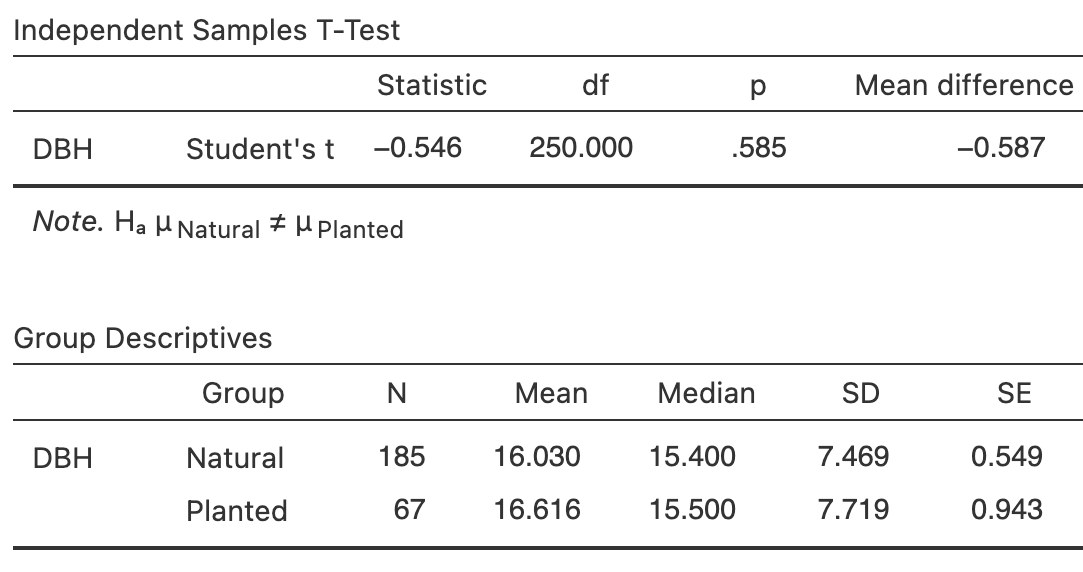
\includegraphics[width=0.75\linewidth]{SoftwareImages/LimeTreesSummary} 

}

\caption{jamovi output for comparing DBH (in cm) for two groups of lime trees,}\label{fig:LimeTreesSummmary}
\end{figure}

\begin{enumerate}
\def\labelenumi{\arabic{enumi}.}
\tightlist
\item
  \emph{How} is the difference between the two groups defined, according to the output?
  \answerbox{2}
\item
  What is the \emph{parameter} according to the output?
  What does this parameter \emph{mean}?
  \answerbox{2}
\item
  \emph{Suppose} the \(95\)\% CI for the difference was computed as~\(-2.7\) to~\(1.5\): very carefully interpret what this would mean in context.
  \answerbox{2}
\item
  \emph{Suppose} the \(95\)\% CI for the difference was computed as~\(0.6\) to~\(4.0\): very carefully interpret what this would mean in context.
  \answerbox{2}
\item
  \emph{Suppose} the \(95\)\% CI for the difference was computed as~\(-4.5\) to~\(-1.6\): very carefully interpret what this would mean in context.
  \answerbox{2}
\end{enumerate}

\section{CIs and tests for mean differences (paired data)}\label{CIImplant}

Guirao et al. (\citeproc{ref-data:Guirao2017:amputees}{2017}) examined the difference between \(2\)-minute walk test score (2MWT) for \(10\)~patients before \emph{and} after receiving a prosthetic implant.
(The 2MWT measures how far participants can walk in two minutes, in metres.)

The 2MWT for ten amputees \emph{with} and \emph{without} an implant are shown in Fig.~\ref{fig:Guirao2MWT}.
The researchers asked:

\begin{quote}
For this type of amputee, is the mean 2MWT \textbf{improved} (i.e., longer distances walked) after using the implant?
\end{quote}

\begin{figure}[hbtp]

{\centering 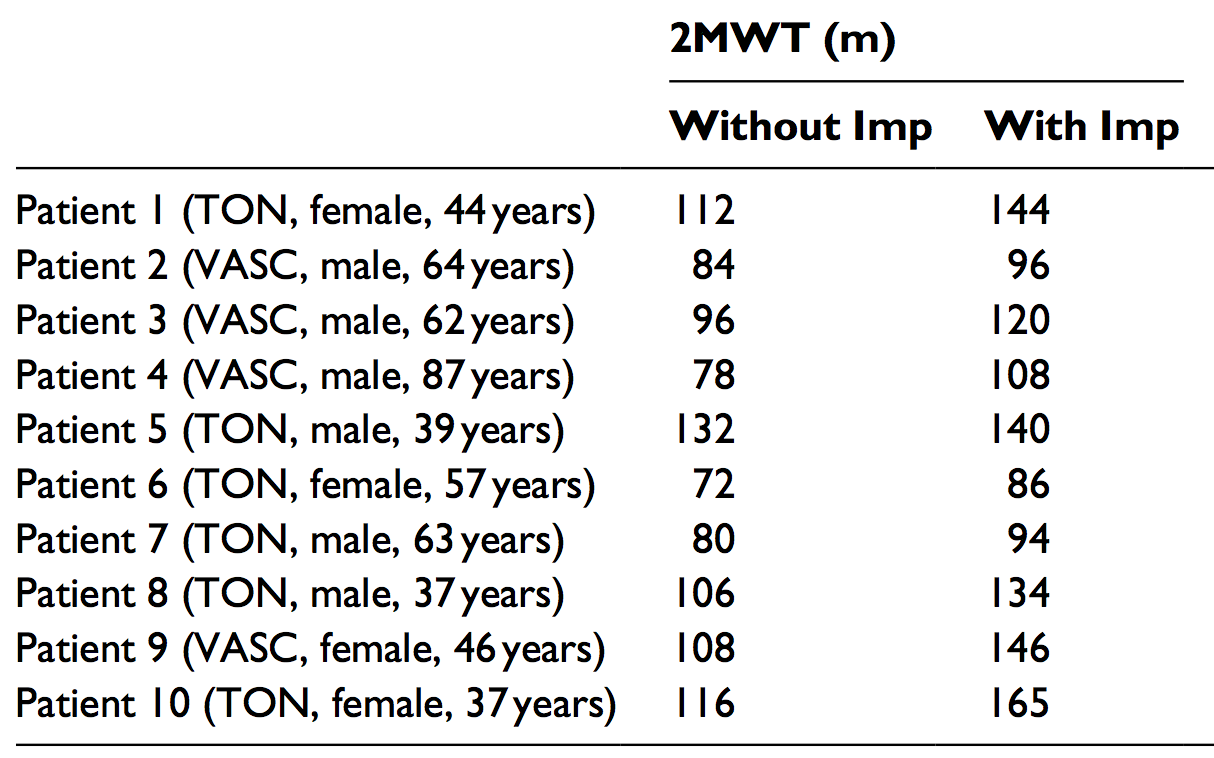
\includegraphics[width=0.7\linewidth]{ArticleImages/Guirao2017-Table2} 

}

\caption{Two-minute Walk Times (2MWT) for $10$ patients with implants (With Imp) and without implants (Without Imp), in metres.}\label{fig:Guirao2MWT}
\end{figure}

\begin{enumerate}
\def\labelenumi{\arabic{enumi}.}
\tightlist
\item
  Suppose the difference were computed as \textbf{With Imp} values \emph{minus} the \textbf{Without Imp} values, what would this measure?
  \answerbox{2}
\item
  Given the software output in Fig.~\ref{fig:2MWTjamovi}, how is the difference defined in jamovi?
  \answerbox{2}
\end{enumerate}

\begin{figure}[hbtp]

{\centering 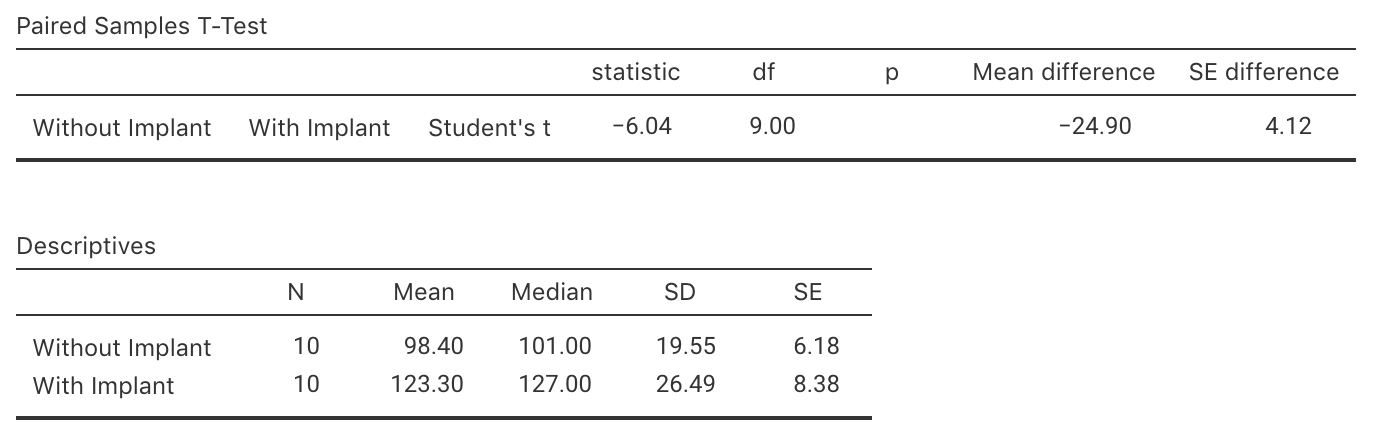
\includegraphics[width=1\linewidth]{ArticleImages/TwoMinuteWalk-edit} 

}

\caption{Output from jamovi for the 2MWT example, partially edited.}\label{fig:2MWTjamovi}
\end{figure}

\begin{enumerate}
\def\labelenumi{\arabic{enumi}.}
\setcounter{enumi}{2}
\tightlist
\item
  What type of RQ is implied: descriptive, relational, repeated-measures or correlational?
  \answerbox{1}
\item
  What do~\(\mu_d\) and~\(\bar{d}\) represent in this context?
  \answerbox{2}
\item
  Explain why these data should be analysed as \emph{paired} data.
  \answerbox{2}
\item
  Compute the \emph{changes} in 2MWT for each patient (write them to the right of the table in Fig.~\ref{fig:Guirao2MWT}).
\item
  Although it doesn't really matter, \emph{why} does it probably makes more sense to compute the \textbf{With Imp} values minus the \textbf{Without Imp} values?
  \answerbox{2}
\item
  Using the statistics mode on your calculator, compute the sample mean difference~\(\bar{d}\) and the sample standard deviation of the differences~\(s_d\).
  \answerbox{2}
\item
  Compute the standard error of the mean difference \(\text{s.e.}(\bar{d})\).
  \answerbox{2}
\item
  Explain the \emph{meaning} of the standard error of the mean difference in this context.
  \answerbox{2}
\item
  If another sample of ten subjects were studied, would the same sample mean difference~\(\bar{d}\) be computed?
  How much variation would be expected in the sample mean differences found from different samples?
  \answerbox{2}
\item
  Draw the approximate sampling distribution of~\(\bar{d}\) that shows how the value of~\(\bar{d}\) varies.
  \answerbox{4}
\item
  Compute an approximate \(95\)\% confidence interval for the population mean difference in 2MWT.
  \answerbox{4}
\item
  Do you think the population 2MWT changes because of the prosthetic, on average?
  \answerbox{3}
\item
  Which of the following is the correct null hypothesis? \tightlist
  \textbf{Why} are the others incorrect?
  Is the test one- or two-tailed?
  What is the alternative hypothesis that is \textbf{consistent with the jamovi output}?
\end{enumerate}

\begin{cols}

\begin{col}{0.4\textwidth}

\begin{itemize}
\tightlist
\item
  \(\mu_{\text{Without Implant}} - \mu_{\text{With implant}} = 0\)
\item
  \(\mu_{\text{Difference}} = 0\)
\item
  \(\mu_{\text{Difference}} > 0\)
\item
  \(\mu_{\text{Without Implant}} = 0\)
\item
  \(\mu_{\text{With implant}} = 0\)
\end{itemize}

\end{col}

\begin{col}{0.05\textwidth}
~


\end{col}

\begin{col}{0.4\textwidth}

\begin{itemize}
\tightlist
\item
  \(\mu_{\text{Without Implant}} - \mu_{\text{With implant}} < 0\)
\item
  \(\mu_{\text{Difference}} < 0\)
\item
  \(\mu_{\text{Without Implant}} < 0\)
\item
  \(\mu_{\text{With implant}} > 0\)
\end{itemize}

\end{col}

\end{cols}

\begin{enumerate}
\def\labelenumi{\arabic{enumi}.}
\setcounter{enumi}{15}
\tightlist
\item
  Write down the value of the \(t\)-statistic, then estimate the \(P\)-value for testing the hypotheses (using Fig.~\ref{fig:2MWTjamovi}).
  \answerbox{3}
\item
  Explain why the \(t\)-score from jamovi is a \emph{negative} value (Fig.~\ref{fig:2MWTjamovi}), but the \(t\)-score from SPSS (Fig.~\ref{fig:2MWTSPSS}) is a \emph{positive} value.
  \answerbox{2}
\item
  Write a statement that communicates the result of the test.
  \answerbox{2}
\item
  What conditions must be met for this test to be valid?
  \answerbox{2}
\item
  Is it reasonable to assume the assumptions are satisfied?
  How does Fig.~\ref{fig:2MWTHisto} help, if at all?
  \answerbox{2}
\end{enumerate}

\begin{figure}[hbtp]

{\centering 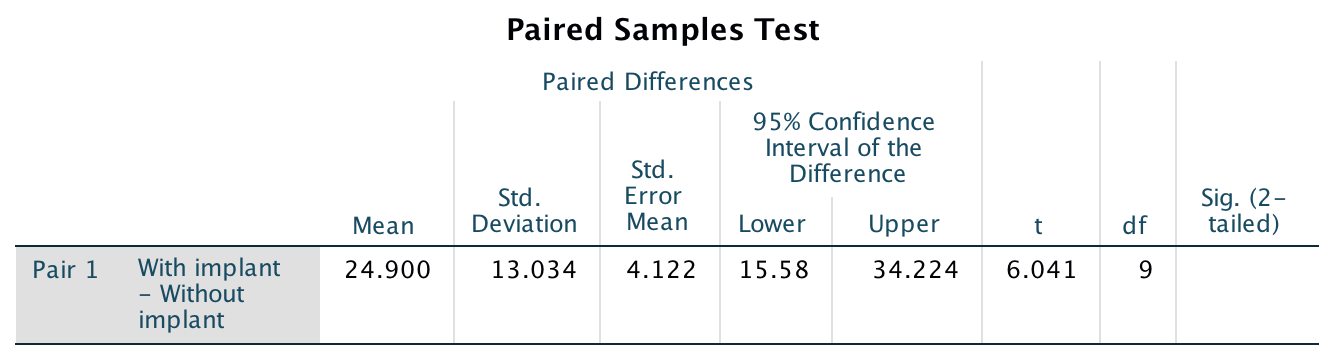
\includegraphics[width=0.95\linewidth]{ArticleImages/Guirao2017-SPSSoutput-blind} 

}

\caption{Output from SPSS for the 2MWT example, partially edited.}\label{fig:2MWTSPSS}
\end{figure}

\begin{figure}[hbtp]

{\centering 
\includegraphics{09-TW9-Tutorial_files/figure-latex/2MWTHisto-1} 

}

\caption{Histogram of differences for the increases in 2MWT with implant.}\label{fig:2MWTHisto}
\end{figure}

\section{CI and test for the ruler-drop}\label{PlanStudy7}

Your tutor \emph{may} decide to do this activity.

\section{CIs and test for difference between two sample means}\label{CIRatLifetimes}

Researchers were interested in the impact of diet on the lifetime of rats:

\begin{quote}
For rats, is the mean lifetime \emph{shorter} for rats on a \emph{free-choice} diet compared to rats on a \emph{healthy, restricted} diet?
\end{quote}

Berger et al. (\citeproc{ref-data:Berger1988:RatsData}{1988}) compared the lifetime of rats on a healthy, restricted diet (\(106\)~rats) and on a free-eating diet (\(89\)~rats).
The data set is large, so only an extract of the data is shown (Fig.~\ref{fig:RatLifetimesDatajamovi}).

\begin{enumerate}
\def\labelenumi{\arabic{enumi}.}
\item
  Explain why this study compares two \emph{independent} groups. \tightlist
  \answerbox{2}
\item
  Carefully define \textbf{parameter} of interest, including the \emph{direction}.
  What does this definition of the difference measure?
  \answerbox{2}
\item
  Use the jamovi output (Fig.~\ref{fig:Berger1988SummaryHTjamovi1}) to prepare a numerical summary table.
  \answerbox{4}
\item
  Use the jamovi output to write down the appropriate \(95\)\%~CI, to estimate the \emph{difference} between the population means.
  \answerbox{4}
\item
  Which of these short statements best communicates this CI?
  \textbf{Why} are the other statements incorrect?

  \begin{enumerate}
  \def\labelenumii{\alph{enumii}.}
  \tightlist
  \item
    The sample mean lifetime is between \(223.34\) and \(346.13\)~days.
  \item
    The difference between the population mean lifetimes is between \(223.34\) and \(346.13\)~days.
  \item
    We are \(95\)\% sure that the difference between the sample mean lifetimes is between \(223.34\) and \(346.13\)~days.
  \item
    We are \(95\)\% sure that the difference between the population mean lifetimes is between \(223.34\) and \(346.13\)~days.
  \item
    If we repeated everything many times, \(95\)\% of the CIs constructed would contain the difference between the population means.
  \end{enumerate}
\item
  The best statement above for communicating the CI is missing an important piece of information.
  Write an improved statement communicating the CI.
  \answerbox{2}
\item
  Explain the difference between the \emph{meaning} of what is displayed in the two graphs in Fig.~\ref{fig:RatsBoxErrorbar}.
  \answerbox{2}
\item
  Write down the hypotheses being tested.
  Is this a one- or a two-tailed test? Explain.
  \answerbox{2}
\item
  What are \emph{two} possible reasons why the sample mean lifetimes of rats on the two diets are different?
  \answerbox{2}
\item
  Write down the \(t\)-score and the appropriate \(P\)-value, using the output in Fig.~\ref{fig:Berger1988SummaryHTjamovi1} .
  \answerbox{3}
\item
  Calculate the \(t\)-score (using the standard error as given in the output), and show it is the same value as given in the output.
  \answerbox{3}
\item
  Make a conclusion, in context.
  \answerbox{2}
\item
  What conditions are necessary for the CI and test to be statistically valid?
  \answerbox{2}
\item
  Is it reasonable to assume these conditions are satisfied?
  How does Fig.~\ref{fig:RatsBoxErrorbar}. help, if at all?
  \answerbox{2}
\item
  What if all these rats only came from only \(20\) litters?
  \answerbox{2}
\end{enumerate}

\begin{figure}[hbtp]

{\centering 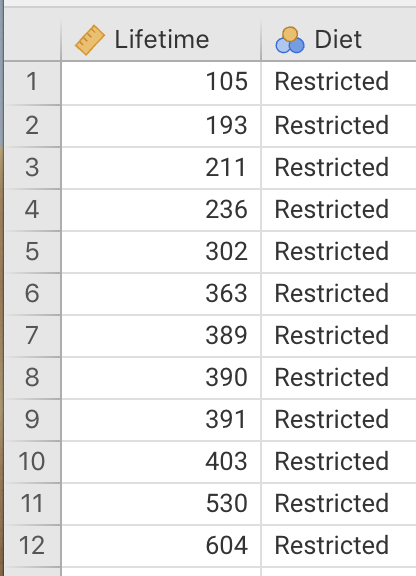
\includegraphics[width=0.27\linewidth]{SoftwareImages/RatLivesData-jamovi} 
\includegraphics[width=0.1\linewidth]{images/SPACER} 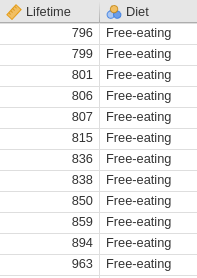
\includegraphics[width=0.26\linewidth]{SoftwareImages/RatLivesData-jamovi2} 

}

\caption{Part of the data for the rat lifetime example (left: the start of the data; right: the end of the data).}\label{fig:RatLifetimesDatajamovi}
\end{figure}

\begin{figure}[hbtp]

{\centering 
\includegraphics[width=0.8\linewidth]{09-TW9-Tutorial_files/figure-latex/RatsBoxErrorbar-1} 

}

\caption{Boxplot (left panel) and error-bar chart (right panel) for the rat lifetime data.}\label{fig:RatsBoxErrorbar}
\end{figure}

\begin{figure}[hbtp]

{\centering 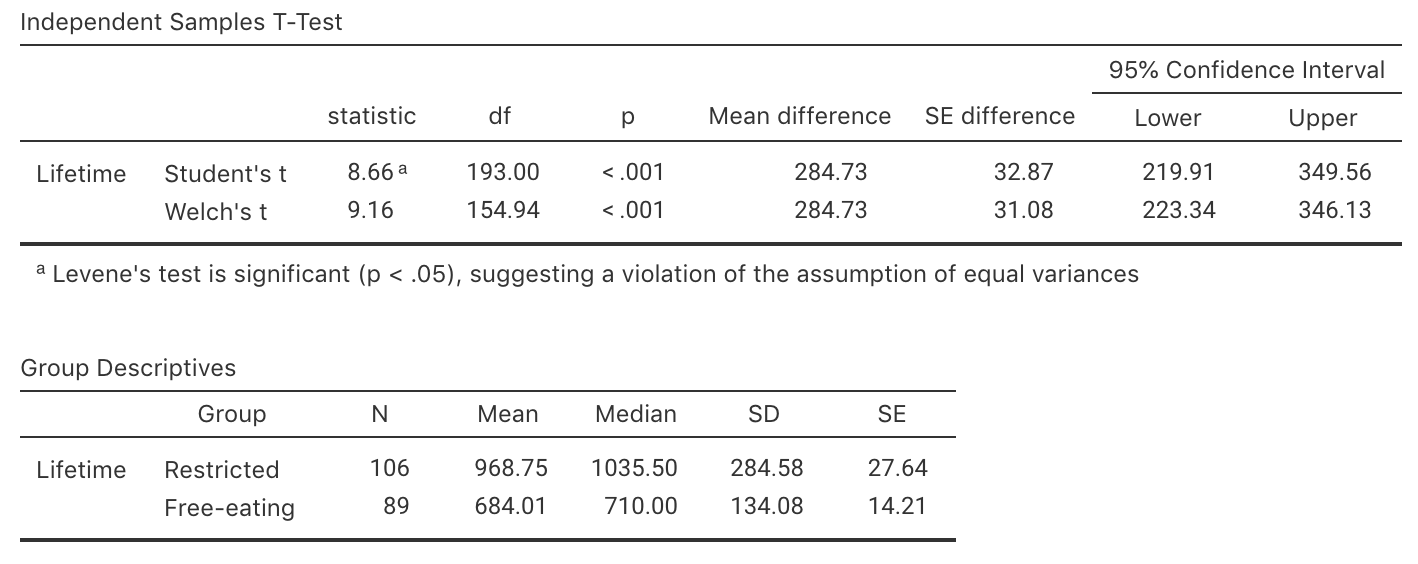
\includegraphics[width=1\linewidth]{SoftwareImages/RatLivesOutput-jamovi} 

}

\caption{The jamovi output summarising the rat lifetimes data.}\label{fig:Berger1988SummaryHTjamovi1}
\end{figure}

\section{\texorpdfstring{\textbf{Optional questions}}{Optional questions}}\label{OptionalTW9}

\begin{optionalBox}{iconmonstr-help-4-240.png}
These questions are \textbf{optional}; e.g., if you need more practice, or you are studying for the exam.
(Answers appear in Sect.~\ref{Lecture9Answers}.)

\end{optionalBox}

\subsection{\texorpdfstring{\textbf{(Optional)} Paired \(t\)-test}{(Optional) Paired t-test}}\label{JumpingInference}

Hébert-Losier et al. (\citeproc{ref-hebert2023effect}{2023}) recorded double-legged jumping distance for~\(80\) healthy people, when they wore shoes and were barefoot.
The data are too large to show here, but use the jamovi output (Fig.~\ref{fig:JumpingDatajamovi}) to answer the following questions.

\begin{enumerate}
\def\labelenumi{\arabic{enumi}.}
\tightlist
\item
  What do the differences \emph{mean} (as given in the output)?
\item
  Create a numerical summary table for the data.
\item
  Determine \(95\)\%~CI for the difference in height of the two jumps.
\item
  Conduct a hypothesis test to determine if a mean difference exists in the population.
\end{enumerate}

\begin{figure}[hbtp]

{\centering 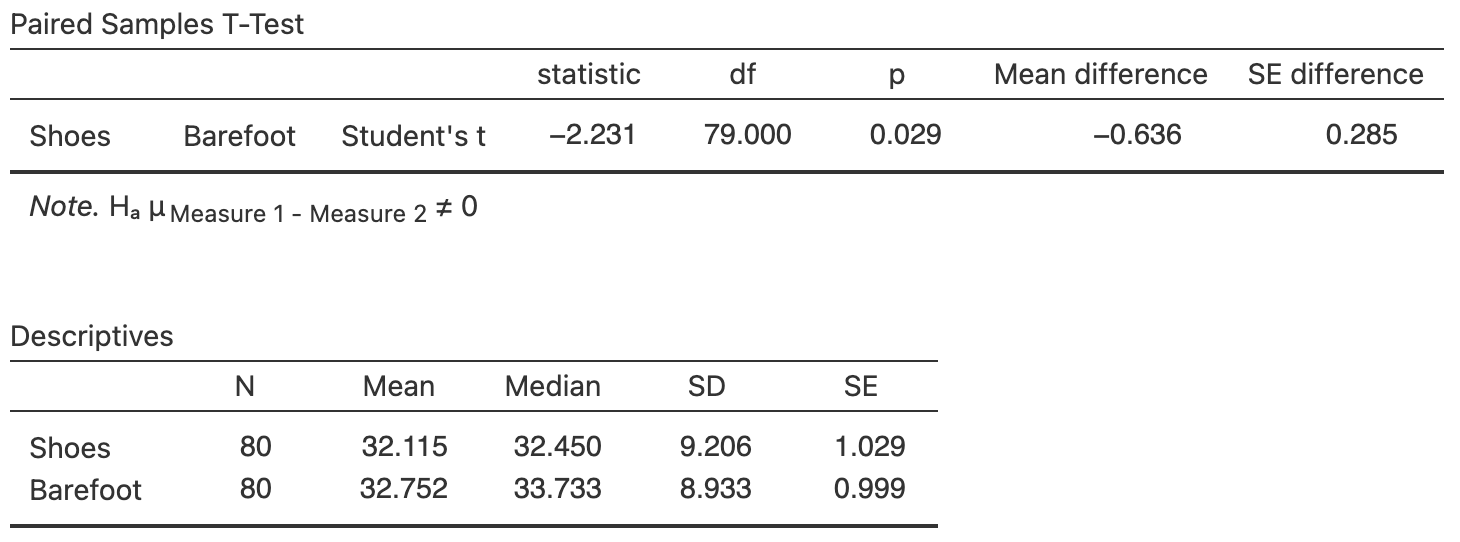
\includegraphics[width=1\linewidth]{SoftwareImages/JumpingOutput} 

}

\caption{The jamovi output summarising the jumping data.}\label{fig:JumpingDatajamovi}
\end{figure}

\subsection{\texorpdfstring{\textbf{(Optional)} Two-sample \(t\)-test}{(Optional) Two-sample t-test}}\label{ReactionTimeInference}

Strayer and Johnston (\citeproc{ref-data:Strayer2001:phones}{2001}) examined the reaction times, while driving, for students from the University of Utah (\citeproc{ref-agresti2007statistics}{Agresti and Franklin 2007}).
In one study, students were randomly allocated to one of two groups:

\begin{itemize}
\tightlist
\item
  one group \emph{used} a mobile phone while driving in a driving simulator; and
\item
  one group \emph{did not use} a mobile phone while driving in a driving simulator.
\end{itemize}

The reaction time for each student was measured.
The data are shown below.
Use the information in Table~\ref{tab:PhoneSummary} to answer this RQ:

\begin{quote}
For students, is there a difference between the mean reaction time while driving when using a mobile phone and when \emph{not} using a mobile phone?
\end{quote}

Be sure to include an approximate \(95\)\%~CI as well as the hypothesis test results.

\begin{table} \centering \centering\caption{\label{tab:PhoneDataTable}Reaction times (in milliseconds) for students using, and not using, mobile phones while driving.}

\fontsize{10}{12}\selectfont
\begin{tabular}[t]{ccccccc}
\toprule
\multicolumn{7}{c}{\textbf{Reaction time: using phone}} \\
\cmidrule(l{3pt}r{3pt}){1-7}
$636$ & $600$ & $609$ & $554$ & $578$ & $688$ & $527$\\
$623$ & $542$ & $559$ & $626$ & $560$ & $679$ & $536$\\
$615$ & $554$ & $595$ & $501$ & $525$ & $960$ & \\
$672$ & $543$ & $565$ & $574$ & $647$ & $558$ & \\
$601$ & $520$ & $573$ & $468$ & $456$ & $482$ & \\
\bottomrule
\end{tabular} \quad\quad 
\begin{tabular}[t]{ccccccc}
\toprule
\multicolumn{7}{c}{\textbf{Reaction time: not using phone}} \\
\cmidrule(l{3pt}r{3pt}){1-7}
$557$ & $506$ & $626$ & $436$ & $617$ & $539$ & $512$\\
$572$ & $648$ & $626$ & $642$ & $528$ & $523$ & $449$\\
$457$ & $485$ & $426$ & $476$ & $578$ & $479$ & \\
$489$ & $610$ & $585$ & $586$ & $472$ & $535$ & \\
$532$ & $444$ & $487$ & $565$ & $485$ & $603$ & \\
\bottomrule
\end{tabular}
\end{table}

\begin{table}

\caption{\label{tab:PhoneSummary}Summary information for the reaction-time data.}
\centering
\begin{tabular}[t]{lcccc}
\toprule
\textbf{ } & \textbf{Mean} & \textbf{Sample size} & \textbf{Std dev.} & \textbf{Std error}\\
\midrule
Using phone & $533.59$ & $32$ & $65.36$ & $11.554$\\
Not using phone & $585.19$ & $32$ & $89.65$ & $15.847$\\
\midrule
Differences & $\phantom{0}51.59$ &  &  & $19.612$\\
\bottomrule
\end{tabular}
\end{table}

\chapter{Teaching Week 10 tutorial}\label{Lecture10}

\begin{objectivesBox}{iconmonstr-target-4-240.png}

You will learn to:

\begin{itemize}
\tightlist
\item
  construct CIs and conduct hypothesis tests for ORs.
\item
  construct CIs and conduct hypothesis tests for the difference between two proportions.
\item
  estimate sample sizes for finding CIs.
\item
  selecting an appropriate analysis for a given situation.
\end{itemize}

\end{objectivesBox}

\begin{assessmentBox}{iconmonstr-text-check-list-lined-240.png}

The Week~10 content is essential for:

\begin{itemize}
\tightlist
\item
  \textbf{Task~2B}, which requires you to \emph{produce CIs and conduct a hypothesis test for your data};
\item
  \textbf{Quiz~4}, which includes questions about \emph{understanding and producing CIs, understanding and conducting hypothesis tests, and estimating sample sizes}; and
\item
  the \textbf{Exam}, which will contain questions about \emph{understanding and producing CIs, understanding and conducting hypothesis tests, and estimating sample sizes}.
\end{itemize}

\end{assessmentBox}

\begin{readBox}{iconmonstr-school-15-240.png}
You will learn and practice the content associated with these chapters of the \href{https://peterkdunn.github.io/SRM-Textbook/}{textbook}:

\begin{itemize}
\tightlist
\item
  \href{https://peterkdunn.github.io/SRM-Textbook/AnalysisOddsRatio.html}{Chapter~31 (CIs and tests: comparing two odds or proportions)}
\item
  \href{https://peterkdunn.github.io/SRM-Textbook/EstimatingSampleSize.html}{Chapter~32 (Finding sample sizes for CIs)}
\item
  \href{https://peterkdunn.github.io/SRM-Textbook/SelectTest.html}{Chapter~34 (Selecting an analysis)}
\end{itemize}

Take careful note of which chapters are covered in this tutorial!

\end{readBox}

\pagebreak

\section{Quick revision}\label{QuickRevision-Tutorial10}

An ecologist is studying two different grasses to help combat soil salinity, by comparing to a new grass (Grass~A) to a native grass (Grass~B).
She uses \(50\)~different sites, allocating the two grasses at random to the sites (\(25\)~sites for each grass).

After \(12\)~months, the ecologist records whether the soil salinity at each site has changed, and hence computes the \emph{odds} that each grass will change the salinity.
She finds a statistically significant difference between the odds in the two groups.

Which of these statements is \emph{consistent} with this conclusion?

\begin{enumerate}
\def\labelenumi{\arabic{enumi}.}
\tightlist
\item
  The \(\text{OR} = 4.1\) and \(P = 0.36\). \tightlist 
\item
  The \(\text{OR} = 4.1\) and \(P = 0.0001\).
\item
  The \(\text{OR} = 0.91\) and \(P = 0.36\).
\item
  The \(\text{OR} = 0.91\) and \(P = 0.0001\).
\end{enumerate}

How would the other statements be interpreted then?
\answerbox{3}

\section{Class discussion}\label{TW10-Class-Discussion}

\begin{discussBox}{iconmonstr-speech-bubble-26-240.png}
\textbf{Discuss}: When comparing two groups, is it better to focus on differences in \emph{proportions}, \emph{odds}, \emph{odds ratios}, or \emph{percentages}?

\end{discussBox}

\section{Consistency and reading output}\label{Consistency}

\begin{importantBox}{iconmonstr-warning-8-240.png}
Consistency between the RQ, hypotheses, the CI, the hypothesis test, and the results is important.
For example: if the RQ is written in terms of \emph{proportions}, then the hypotheses, CI and so forth should also be written in terms of \emph{proportions}.\medskip

In addition: explaining exactly what the statistic and the CI are estimating (the \textbf{parameter}) is \textbf{very} important.

\end{importantBox}

Suppose a researcher asked the RQ:

\begin{quote}
For Australians, are the \emph{odds} of people with mosquito bites the same for people sitting near a citronella candle as for people sitting near an ordinary wax candle?
\end{quote}

\begin{enumerate}
\def\labelenumi{\arabic{enumi}.}
\item
  Which would be the appropriate null hypothesis? \tightlist
  \null

  \begin{enumerate}
  \def\labelenumii{\alph{enumii}.}
  \tightlist
  \item
    The odds of a person being bitten by a mosquito is the same for people near citronella candles and wax candles.
  \item
    The proportion of people being bitten by a mosquito is the same for people near citronella candles and wax candles.
  \item
    Either of the above.
  \end{enumerate}
\item
  Which would be the appropriate CI to produce?
  \null

  \begin{enumerate}
  \def\labelenumii{\alph{enumii}.}
  \tightlist
  \item
    A CI for the odds ratio.
  \item
    A CI for the difference in proportions.
  \item
    Either of the above.
  \end{enumerate}
\item
  Which would be the appropriate hypothesis test?
  \null

  \begin{enumerate}
  \def\labelenumii{\alph{enumii}.}
  \tightlist
  \item
    A hypothesis tests for the difference between proportions.
  \item
    A hypothesis tests for the odds ratio.
  \item
    Either of the above.
  \end{enumerate}
\end{enumerate}

The jamovi output is shown in Fig.~\ref{fig:MosquitoBitesjamovi}.

\begin{figure}[hbtp]

{\centering 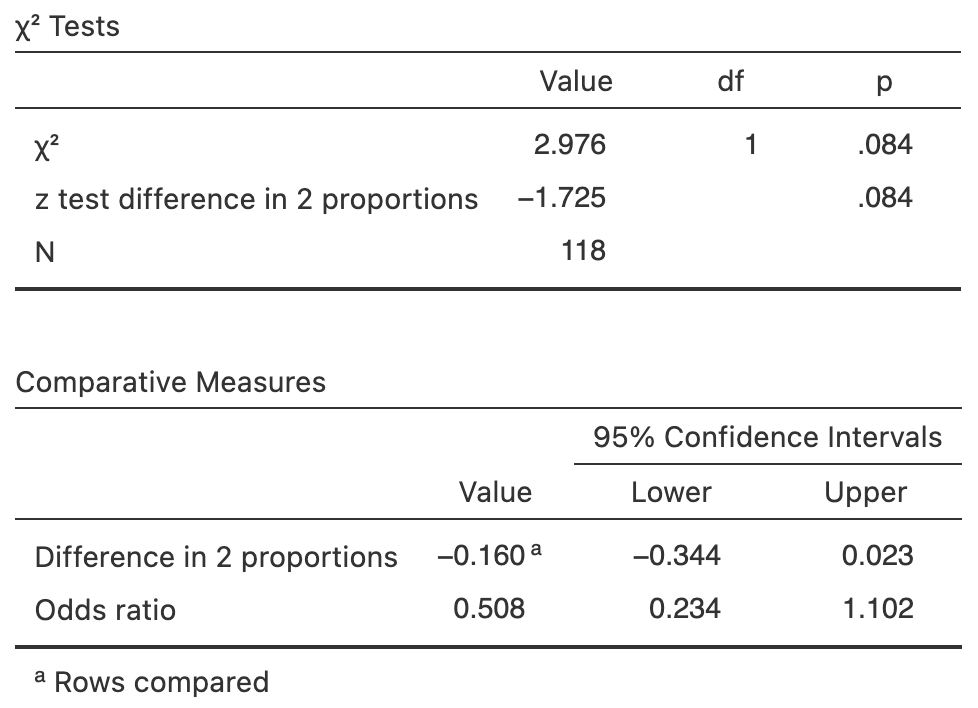
\includegraphics[width=0.65\linewidth]{SoftwareImages/MosquitoBites} 

}

\caption{Mosquito bites when near different types of candles.}\label{fig:MosquitoBitesjamovi}
\end{figure}

\begin{enumerate}
\def\labelenumi{\arabic{enumi}.}
\setcounter{enumi}{3}
\tightlist
\item
  What is the odds ratio? \tightlist
  \answerbox{1}
\item
  Very carefully, explain what this odds ratio \textbf{means} in context.
  \answerbox{2}
\item
  The output also shows the difference between proportions.
  Very carefully, explain what this difference \textbf{means} in context.
  \answerbox{2}
\item
  In the study, the odds that someone received a mosquito bite when a \emph{wax} candle was being used was~\(2.167\).
  What are the odds that someone in the study received a mosquito bite when a \emph{citronella} candle was used?
  \answerbox{2}
\item
  The \(95\)\% CI for the odds ratio is from~\(0.234\) to~\(1.102\).
  Very carefully interpret what this means in context.
  \answerbox{2}
\item
  \emph{Suppose} the \(95\)\% CI for the odds ratio was from~\(0.11\) to~\(0.94\).
  Very carefully interpret what this would mean in context.
  \answerbox{2}
\item
  \emph{Suppose} the \(95\)\% CI for the odds ratio was from~\(1.28\) to~\(4.13\).
  Very carefully interpret what this would mean in context.
  \answerbox{2}
\item
  Check that the CIs are statistically valid.
  \answerbox{2}
\end{enumerate}

\section{CI and test for odds ratios}\label{OddsSoftware}

The timing of pubertal maturation can vary, which can have impacts upon behaviour.
Duncan et al. (\citeproc{ref-data:duncan:maturity}{1985}) studied `the relationships between maturational timing and body image, school behavior, and deviance.'
Sample data were collected from

\begin{quote}
\ldots children and youth of the entire United States drawn by the National Center for Health Statistics\ldots{} known as the National Health Examination Survey (1966--1970).
Data were collected on\ldots{} adolescents' physical and psychological status\ldots{}
\end{quote}

The researchers asked the RQ;

\begin{quote}
For US children, is the odds of a boy maturing late the \emph{same} as the odds of a girl maturing late?
\end{quote}

Part of the data are shown entered into jamovi (Fig.~\ref{fig:MaturationData-jamova-SPSS})

\begin{figure}[hbtp]

{\centering 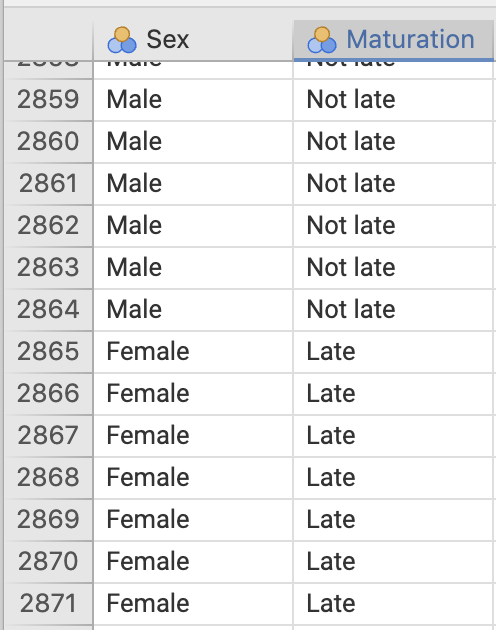
\includegraphics[width=0.33\linewidth]{SoftwareImages/BoysMatureData-jamovi} 

}

\caption{Some of the maturation-data entered into jamovi.}\label{fig:MaturationData-jamova-SPSS}
\end{figure}

\begin{enumerate}
\def\labelenumi{\arabic{enumi}.}
\tightlist
\item
  For the \(2\,864\) males in the sample, \(352\) were classified as maturing late.
  For the girls, \(336\) of the \(2\,664\) matured late.
  Use this information to construct a two-way table of sex against maturation time (Table~\ref{tab:MaturationData}).
\end{enumerate}

\begin{table}
\centering
\caption{\label{tab:MaturationData}Maturation and gender.}
\centering
\fontsize{10}{12}\selectfont
\begin{tabular}[t]{>{}lrrr}
\toprule
\textbf{ } & \textbf{Matured late} & \textbf{Did not mature late} & \textbf{Total}\\
\midrule
\textbf{Males} &  &  & \\
\textbf{Females} &  &  & \\
\midrule\\
\textbf{\textbf{Total}} & \textbf{} & \textbf{} & \textbf{5528}\\
\bottomrule
\end{tabular}
\end{table}

\begin{enumerate}
\def\labelenumi{\arabic{enumi}.}
\setcounter{enumi}{1}
\tightlist
\item
  What graphical summary could be used to display the information?
  Sketch this display.
  \answerbox{4}
\item
  Among the boys, compute the \emph{odds} of maturing late.
  Interpret this value.
  \answerbox{2}
\item
  Among the girls, compute the \emph{odds} of maturing late.
  Interpret this value.
  \answerbox{2}
\item
  From the table, compute the odds ratio of a boy maturing late compared to a girl maturing late.
  Interpret this value, using the software output (Fig.~\ref{fig:BoysMaturejamovi}).
  \answerbox{2}
\item
  What is the \textbf{parameter} of interest (make sure you specify the direction)?
  \answerbox{2}
\item
  Write down the OR and the \(95\)\%~CI for the OR from the jamovi output.
  What does it mean?
  \answerbox{2}
\item
  Compile the numerical summary table for these data (Table~\ref{tab:MaturationSummary}).
\item
  Are boys generally more likely to mature later than girls?
  Perform a hypothesis test.
  \answerbox{4}
\end{enumerate}

\begin{figure}[hbtp]

{\centering 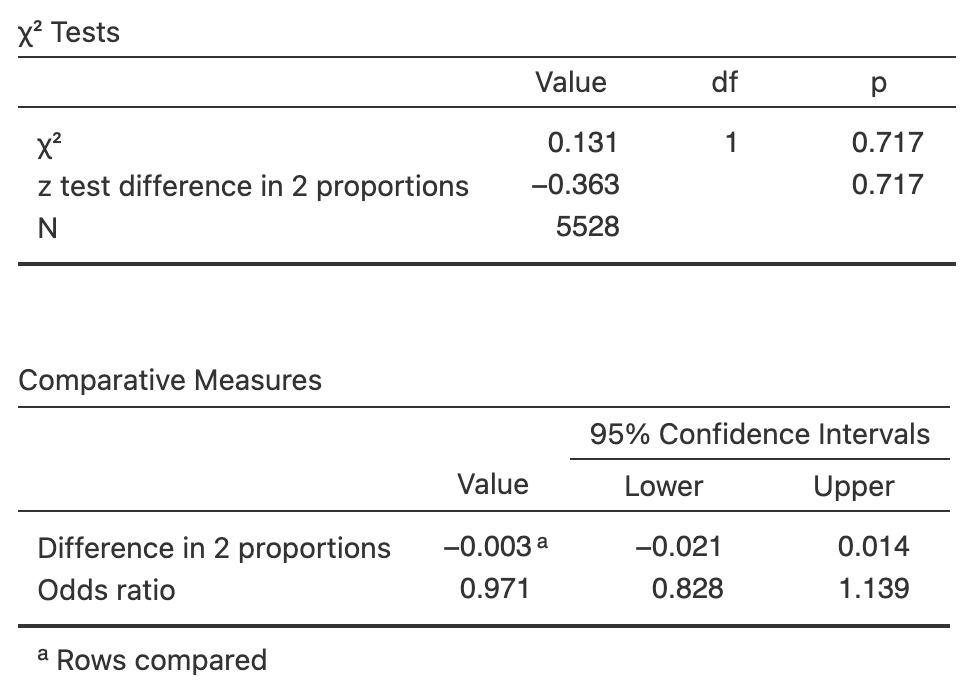
\includegraphics[width=0.55\linewidth]{SoftwareImages/BoysMatureTestsCI-jamovi} 

}

\caption{The jamovi output from the maturation study}\label{fig:BoysMaturejamovi}
\end{figure}



\begin{table}
\centering
\caption{\label{tab:MaturationSummary}Maturation and gender: numerical summary}
\centering
\fontsize{10}{12}\selectfont
\begin{tabular}[t]{>{}llll}
\toprule
\textbf{ } & \textbf{Proportion maturing late} & \textbf{Odds  maturing late} & \textbf{Sample size}\\
\midrule
\textbf{Males} &  &  & \\
\textbf{Females} &  &  & \\
\midrule
\textbf{} & Diff.: & Odds ratio: & \\
\bottomrule
\end{tabular}
\end{table}

\section{CIs and tests for ORs}\label{TestsForORs}

Singh and Prasad (\citeproc{ref-data:Singh:lowerlimb}{2016}) examined the mortality rates of lower-limb amputation, and factors that may be associated with mortality.
As part of the study, the researchers recorded the five-year mortality rate (the number of amputees who died within five years of amputation) and whether or not the person used an artificial limb.

The RQ was:

\begin{quote}
For this type of amputees, is the odds of being alive after five years the same for those who used an artificial limb, and those who did not?
\end{quote}

A total of \(105\) subjects were used: \(35\) died within five years, and \(70\) were still alive after five years.
In addition, \(65\) subjects used an artificial limb, and \(40\) did not.

\begin{enumerate}
\def\labelenumi{\arabic{enumi}.}
\tightlist
\item
  After five years, \(49\) people using an artificial limb were alive.
  Construct the \(2\times 2\) table (Table~\ref{tab:ArtLimbMortality}) displaying the number of people alive or dead after five years (in columns, say) and whether or not they used an artificial limb or not (in rows).
\end{enumerate}

\begin{table}
\centering
\caption{\label{tab:ArtLimbMortality}Five-year mortality for artifical limb users.}
\centering
\fontsize{10}{12}\selectfont
\begin{tabular}[t]{>{}lrrr}
\toprule
\textbf{ } & \textbf{Alive} & \textbf{Dead} & \textbf{Total}\\
\midrule
\textbf{Used artificial limb} &  &  & \\
\addlinespace
\textbf{Did not use artificial limb} &  &  & \\
\midrule
\addlinespace
\textbf{\textbf{Total}} & \textbf{} & \textbf{} & \textbf{105}\\
\bottomrule
\end{tabular}
\end{table}

\begin{enumerate}
\def\labelenumi{\arabic{enumi}.}
\setcounter{enumi}{1}
\item
  In Table~\ref{tab:ArtLimbMortality}, \emph{why} is the use (or not) of artificial limbs listed in the \emph{rows} (rather than the \emph{columns})?
  \answerbox{2}
\item
  For a person using an artificial limb, compute the odds of being alive after five years.
  For a person \emph{not} using an artificial limb, compute the odds of being alive after five years.
  Then compute the odds ratio, complete Table~\ref{tab:ArtLimbSummary}, and carefully explain what the OR means.
  \answerbox{4}
\item
  Write down the \(95\)\%~CI for the population OR using the software output (Fig.~\ref{fig:limbsOutputjamovi}).
  \answerbox{2}
\item
  Perform a hypothesis test to compare the odds of being alive after five years for both groups (Fig.~\ref{fig:limbsOutputjamovi}):

  \begin{enumerate}
  \def\labelenumii{\alph{enumii}.}
  \tightlist
  \item
    Write the hypotheses.
    \answerbox{2}
  \item
    Write down the value of~\(\chi^2\).
    \answerbox{2}
  \item
    What \(z\)-score is this equivalent to?
    \answerbox{2}
  \item
    What is the approximate \(P\)-value using the \(68\)--\(95\)--\(99.7\) rule?
    \answerbox{2}
  \item
    What is the exact \(P\)-value as reported by software?
    \answerbox{2}
  \item
    Write a conclusion.
    \answerbox{2}
  \end{enumerate}
\end{enumerate}

\begin{table}
\centering
\caption{\label{tab:ArtLimbSummary}Five-year mortality and use of an artificial limb: numerical summary.}
\centering
\fontsize{10}{12}\selectfont
\begin{tabular}[t]{>{}llll}
\toprule
\multicolumn{1}{r}{\textbf{ }} & \multicolumn{1}{r}{\textbf{Proportion alive}} & \multicolumn{1}{r}{\textbf{Odds of being alive}} & \multicolumn{1}{r}{\textbf{Sample}} \\
\textbf{ } & \textbf{after 5 years} & \textbf{after 5 years} & \textbf{size}\\
\midrule
\textbf{Use artificial limb} &  &  & \\
\addlinespace
\textbf{Did not use artifical limb} &  &  & \\
\midrule\\
\addlinespace
\textbf{} & Diff.: & Odds ratio: & \\
\bottomrule
\end{tabular}
\end{table}

\begin{figure}[hbtp]

{\centering 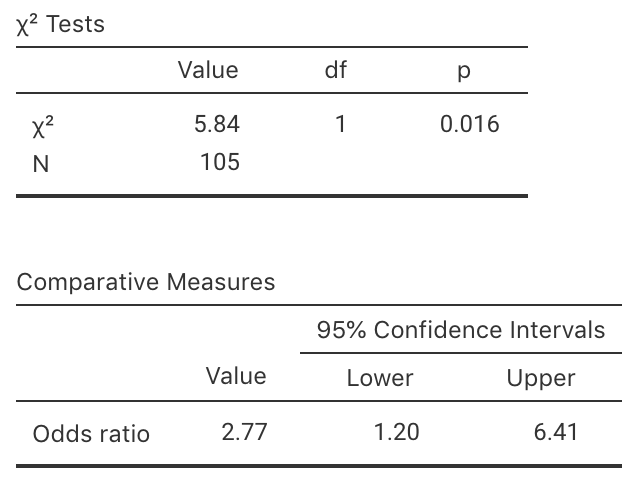
\includegraphics[width=0.5\linewidth]{SoftwareImages/Singh2016-ChiSq-jamovi} 

}

\caption{The jamovi output for the question on lower-limb amputees.}\label{fig:limbsOutputjamovi}
\end{figure}

\section{Identify the correct analysis}\label{IdentifyCorrectAnalyses}

For each of the following scenarios:

\begin{enumerate}
\def\labelenumi{\alph{enumi}.}
\item
  determine the appropriate method of analysis (if none are appropriate, say so then identify the correct analysis):

  \begin{enumerate}
  \def\labelenumii{\roman{enumii}.}
  \tightlist
  \item
    A \(\chi^2\) test;
  \item
    A \(z\)-test for comparing two proportions;
  \item
    A paired \(t\)-test for the mean difference;
  \item
    A two-sample \(t\)-test
  \item
    None of the above.
  \end{enumerate}
\item
  carefully define the \textbf{parameter} of interest.
\end{enumerate}

\begin{enumerate}
\def\labelenumi{\arabic{enumi}.}
\tightlist
\item
  Populations of the scaled quail have been decreasing.
  An observational research study (\citeproc{ref-data:pleasant:quail}{Pleasant et al. 2006}) examined the nests of scaled quails to determine some of the reasons for this decline.
\end{enumerate}

In each nest, the researchers recorded the maximum temperature during the first \(21\)~days posthatch.
Two groups of nests were compared: when the hen was present at \(21\)~days posthatch (\(n = 17\) nests), and when the hen was absent at \(21\)~days posthatch (\(n = 37\) nests).
The aim was to see if the \emph{mean} maximum temperature was different for both groups (hen present; hen absent).

What is the appropriate method of analysis?
Carefully define the parameter of interest.
\answerbox{2}

\begin{enumerate}
\def\labelenumi{\arabic{enumi}.}
\setcounter{enumi}{1}
\item
  Many studies have observed an association between the presence of airborne allergens and people reporting asthma (e.g., Targonski et al., 1995). To better understand the risks of airborne allergens, a study examined the records for numerous people who died of asthma.

  For each person, they recorded the sex of the person (female or male) who died of asthma, and whether they died in pollen season or non-pollen season.

  The aim was to see if the \textbf{odds} of dying of of asthma in pollen season was the same for females and males.

  What is the appropriate method of analysis?
  Carefully define the parameter of interest.
  \answerbox{2}
\item
  An experimental study (\citeproc{ref-data:VanLeit2002:ChildrenWithDisabilities}{VanLeit and Crowe 2002}) ``evaluated the impact of an 8-week psychosocial occupational therapy intervention program for mothers who have children with disabilities'' (p.~402).

  Each mother was evaluated on their satisfaction in how they are spending their time, using the (quantitative) TUA scale.
  Mothers have their TUA score measured \emph{before} and \emph{after} the intervention to see if the intervention made a difference to TUA scores (on average).

  What is the appropriate method of analysis?
  Carefully define the parameter of interest.
  \answerbox{2}
\item
  A experimental study (\citeproc{ref-data:Ingenbleek2012:Vegetarianism}{Ingenbleek and McCully 2012}) compared vegetarians to non-vegetarians on many criteria.

  In one example, each person in the study was described as vegetarian or not, and each person's serum lipids concentration (in mmol/L) was assessed.

  What is the appropriate method of analysis?
  Carefully define the parameter of interest.
  \answerbox{2}
\item
  A study compared the proportion of females in retail working overtime, to the proportion of males on retail working overtime.

  What is the appropriate method of analysis?
  Carefully define the parameter of interest.
  \answerbox{2}
\item
  A study compared the relationship between the VO2 max (a measure of an individual of an individual physical fitness) and \(3\)~km running velocity, for a set of male long-distance runners.

  What is the appropriate method of analysis?
  Carefully define the parameter of interest.
  \answerbox{2}
\end{enumerate}

\section{Sample size calculations}\label{RoomWidthCISampleSize}

\begin{videoSolutionBox}{iconmonstr-youtube-10-240.png}
This question has a video solution in the online book, so you can hear and see the solution.

\end{videoSolutionBox}

Shortly after metric units were introduced to Australia in 1977, a lecturer wondered how accurately students could estimate lengths using the metric measurements (\citeproc{ref-data:hand:handbook}{Hand et al. 1996}).

The aim of the study was to determine if, on average, students could correctly guess the width of the hall (which was \(13.1\,\text{m}\)).

The \(44\) individual students' guesses had a standard deviation of \(7.145\,\text{m}\).
Suppose the Professor wanted to try the study again with another groups of students, and wanted to estimate the population mean to within \(0.5\,\text{m}\).

What size sample would Prof.~Lewis need?
\answerbox{4}

\chapter{Teaching Week 11 tutorial}\label{Lecture11}

\begin{objectivesBox}{iconmonstr-target-4-240.png}

You will learn to:

\begin{itemize}
\tightlist
\item
  read and understand research.
\item
  write about research.
\end{itemize}

\end{objectivesBox}

\begin{assessmentBox}{iconmonstr-text-check-list-lined-240.png}

The Week~11 content is essential for:

\begin{itemize}
\tightlist
\item
  \textbf{Task~2B}, which requires you to \emph{write about your own research};
\item
  \textbf{Quiz~4}, which includes questions about \emph{understanding the language of research, and understanding extracts from published research}; and
\item
  the \textbf{Exam}, which will contain questions about \emph{understanding the language of research, and understanding extracts from published research}.
\end{itemize}

\end{assessmentBox}

\begin{readBox}{iconmonstr-school-15-240.png}

You will learn and practice the content associated with these chapters of the \href{https://peterkdunn.github.io/SRM-Textbook/}{textbook}:

\begin{itemize}
\tightlist
\item
  \href{https://peterkdunn.github.io/SRM-Textbook/WritingResearch.html}{Chapter~35 (Reporting and writing research)}.
\item
  \href{https://peterkdunn.github.io/SRM-Textbook/Reading.html}{Chapter~36 (Reading and critiquing research)}.
\end{itemize}

\end{readBox}

\pagebreak

\section{Quick revision}\label{QuickRevision-Tutorial11}

In a study of high strength--high ductile concrete, Ranade et al. (\citeproc{ref-data:Ranada2015:Concrete}{2015}) measured (among other things) the load required to create the first visible cracks in concrete samples under various strains rates.

Under a strain rate of \(10\,\text{s}^{-1}\), the \(n = 6\) concrete samples produced a \textbf{mean} first-crack strength of \(12.4\,\text{MPa}\) with a \textbf{standard deviation} of \(2.8\,\text{MPa}\).

One student computes the approximate \(95\)\%~CI for the mean first-crack strength as \(12.4\pm 2.8\,\text{MPa}\).
Another student computes the approximate \(95\)\%~CI for the mean first-crack strength as \(12.4\pm (2\times 2.8)\), or from~\(6.8\) to~\(18.0\,\text{MPa}\).

\emph{Both} students are incorrect.

\begin{enumerate}
\def\labelenumi{\arabic{enumi}.}
\tightlist
\item
  Explain \emph{why} Student~1 is incorrect, and explain what the student actually calculated.
  \answerbox{4}
\item
  Explain \emph{why} Student~2 is incorrect, and explain what the student actually calculated.
  \answerbox{4}
\item
  Compute the correct (approximate) \(95\)\%~CI.
  \answerbox{4}
\end{enumerate}

\section{Class discussion}\label{TW11-Class-Discussion}

\begin{discussBox}{iconmonstr-speech-bubble-26-240.png}
\textbf{Discuss}: A `statistically significant' result means a real discrepancy or effect.

\end{discussBox}

\section{Critiquing past students' reports 1}\label{CritiqueReports1}

The extracts below are from an actual student Project Report.
Critique these extracts, and suggest better ways of communicating the information.

From a study comparing the mean distance an iron golf club and a wooden golf club can hit the ball:

\begin{itemize}
\tightlist
\item
  \textbf{Research question}:
  For casual golfers, will using a metal club rather than a wooden club result in the ball travelling a further distance?
  \answerbox{4}
\item
  \textbf{Summaries}:
  The paired means are different with the iron golf club being moderately higher than the wooden club
  \answerbox{4}
\item
  \textbf{Results (1)}:
  The \(95\)\%~CI for the difference in distance in metres (wooden verse iron) differs from \(34.74\) -- \(43.25\) further for shots with the Iron
  \answerbox{4}
\item
  \textbf{Results (2)}:
  Very strong evidence exists in the paired sample (paired \(t = 18.406\); \(n = 50\); two tailed; \(P = 0.000\)) of a population mean difference between the wooden and iron golf clubs\ldots{}
  \answerbox{4}
\end{itemize}

\section{Critiquing past students' reports 2}\label{CritiqueReports2}

The extracts below are from an actual student Project Report.
Critique these extracts, and suggest better ways of communicating the information.

From a study comparing resting heart rates between male and female SCI110 students:

\begin{itemize}
\tightlist
\item
  \textbf{Null hypothesis}:
  Among current UniSC students studying SCI110, male and female resting heart rates are the same.
  \answerbox{4}
\item
  \textbf{Results}:
  The sample presents evidence (\(\chi^2 = 30.0\); two tailed \(P = 0.517\)) that the mean resting heart rate does not have a significant difference between males and females (males mean: \(72.6\)~bpm; females mean: \(77.2\)~bpm).
  \answerbox{4}
\end{itemize}

\section{Tests for ORs}\label{ORAirways}

\begin{videoSolutionBox}{iconmonstr-youtube-10-240.png}
This question has a video solution in the online book, so you can hear and see the solution.

\end{videoSolutionBox}

A study (\citeproc{ref-data:Tanagawa:AirwayDevices}{Tanagawa and Shigematsu 1998}) examined the choice of airway devices used for nontraumatic, out-of-hospital cardiac arrest patients, to evaluate the success and failure of insertion for various devices.

The data for success and failure at insertion is given in Table \ref{tab:AirwayTab}, taken from available patient documentation.

\begin{table}
\centering
\caption{\label{tab:AirwayTab}Data from the airways study.}
\centering
\fontsize{10}{12}\selectfont
\begin{tabular}[t]{>{}lrr}
\toprule
\textbf{ } & \textbf{Succeed} & \textbf{Fail}\\
\midrule
\textbf{Esophageal gastric tube airway (EGTA)} & 545 & 49\\
\textbf{Laryngeal mask (LM)} & 2701 & 315\\
\bottomrule
\end{tabular}
\end{table}

\begin{enumerate}
\def\labelenumi{\arabic{enumi}.}
\tightlist
\item
  Define~\(p\) as the population proportion of successful attempts at insertion. \tightlist
  Write the hypotheses to be tested.
  \answerbox{4}
\item
  Use the software output in Fig.~\ref{fig:Tanagawa1998jamoviCrossTabs} to test the hypotheses.
  Write a proper conclusion to communicate the results.
  \answerbox{4}
\item
  Are the results likely to be statistically valid?
  Explain.
  \answerbox{2}
\item
  The study was designed to enable medics to choose the best airway device.
  Would you recommend EGTA or LM?
  Why?
  Would you like any more information before making your choice?
  Explain.
  \answerbox{4}
\end{enumerate}

\begin{figure}[hbtp]

{\centering 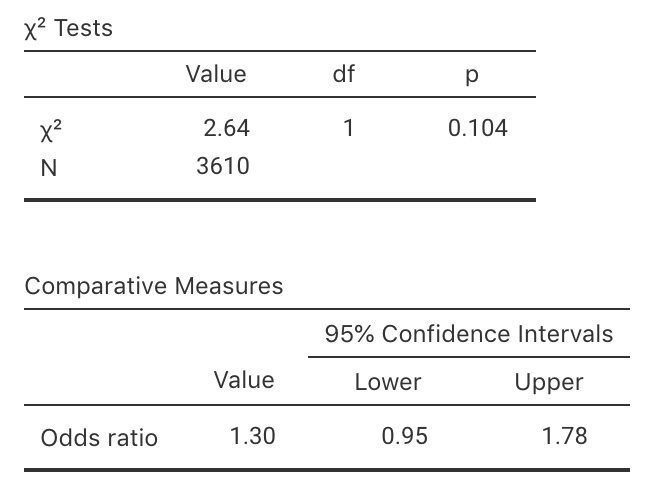
\includegraphics[width=0.55\linewidth]{SoftwareImages/Tanagawa1998jamoviCrossTabs} 

}

\caption{The jamovi output for the table from Tanagawa and Shigematsu (1998).}\label{fig:Tanagawa1998jamoviCrossTabs}
\end{figure}

\section{Critiquing past students' reports 3}\label{CritiqueReports3}

The extracts below are from an actual student Project Report.
Critique these extracts, and suggest better ways of communicating the information.

From a study comparing the size of lilly pilly leaves on different sides of the tree:

\begin{itemize}
\tightlist
\item
  \textbf{Research question}:
  Among Weeping Lily Pily trees located at the University of the Sunshine Coast, do leaves that grow on the sunrise (east) side become longer than those growing on the sunset (west) side of the tree?
  \answerbox{4}
\item
  \textbf{Null hypothesis}:
  The leaves on the east and west sides of Weeping Lily Pily trees are same, therefore no relationship exists between the sunset (east) and sunrise (west) side of the tree and leaf length.
  \answerbox{4}
\item
  \textbf{Results}: The table of results in Fig.~\ref{fig:BreeTable}.
  \answerbox{4}
\item
  \textbf{Methods}:
  Chose the \(5\)~trees at the university that receive both easterly and westerly sunlight conditions
  The \(4\)th leaf on the branch will be chosen \(5\)~times on each side of the tree
  \answerbox{4}
\end{itemize}

\begin{figure}[hbtp]

{\centering 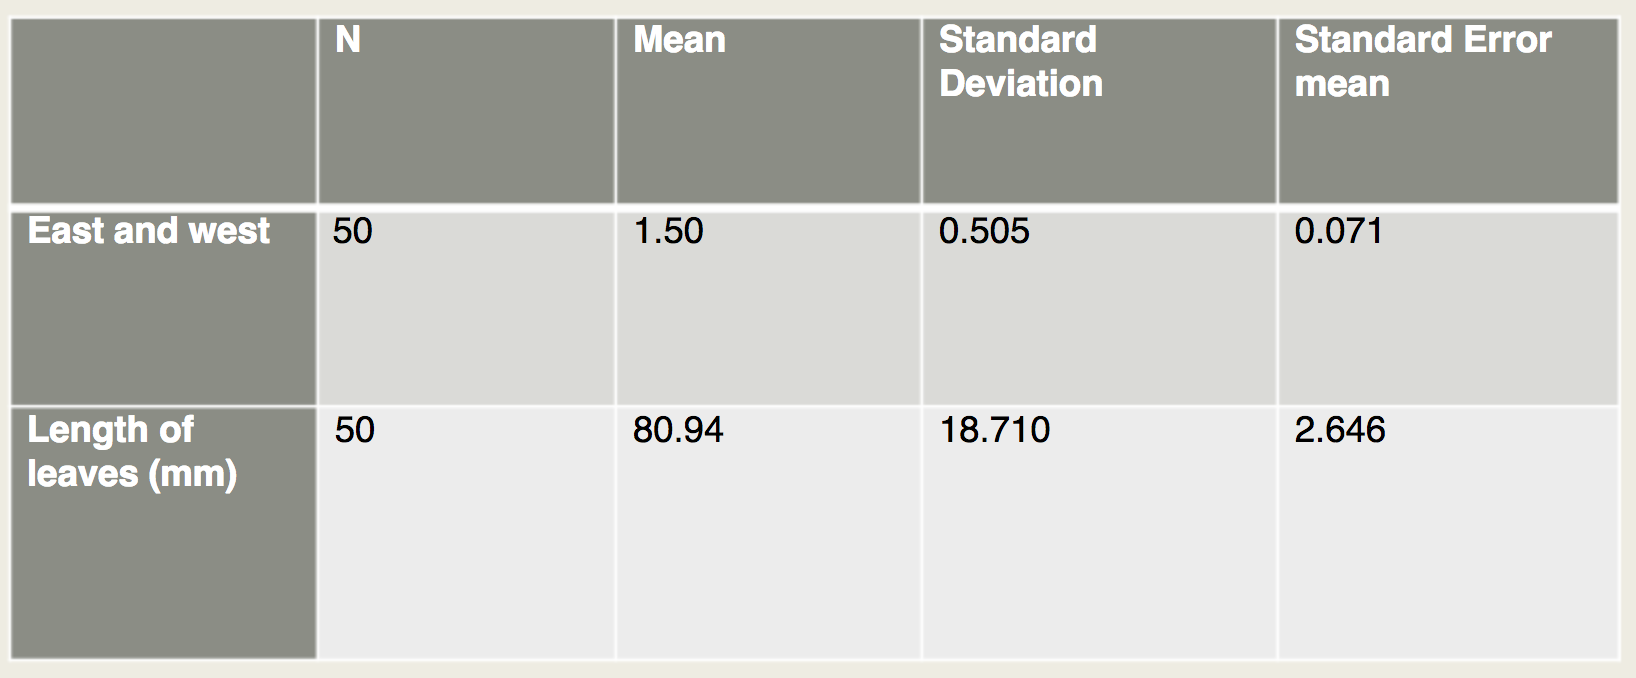
\includegraphics[width=0.7\linewidth]{ProjectImages/BreeTable} 

}

\caption{A table from a student project.}\label{fig:BreeTable}
\end{figure}

\section{Critiquing past students' reports 4}\label{CritiqueReports4}

The extracts below (including typos) are from an actual student Project Report.
Critique these extracts, and suggest better ways of communicating the information.

From a study comparing how well sports-playing students can estimate distance compared to non-sports-playing students:

\begin{itemize}
\item
  \textbf{Research question}:
  Among UniSC Sippy Downs students, are individuals who regularly play sports have closer estimations to the actual measurement when identifying the width of a regular path compared to individuals who don't play sports regularly?
  \answerbox{4}
\item
  \textbf{Null hypothesis}:
  The Null Hypophysis for our research question is that students who play sports regularly at the UniSC Sippy down campus have an increased level of perception when it comes to estimating distances.
  \answerbox{4}
\item
  \textbf{Results}:
  This sample presents strong evidence in support of the Null Hypothesis that sport status has an affect on distance estimation (regular played sport: mean \(176.36\) and non regular played sport: mean \(172.34\)).
  \answerbox{4}
\item
  \textbf{Discussion}:
  From our original research question we have concluded that it supports the Null Hypothesis as it has a large \(P\)-value (\(0.36\): one-tailed). Therefore we have proven that playing sports regularly has an effect on the accuracy of distance estimation.
  \answerbox{4}
\end{itemize}

\chapter{Teaching Week 12 tutorial}\label{Lecture12}

\begin{objectivesBox}{iconmonstr-target-4-240.png}

You will learn to:

\begin{itemize}
\tightlist
\item
  construct CIs and conduct hypothesis tests for correlation coefficients.
\item
  understand linear equations.
\item
  estimate the parameters in simple linear regression models.
\item
  find the parameters in simple linear regression models from software.
\item
  construct CIs and conduct hypothesis tests for regression coefficients.
\end{itemize}

\end{objectivesBox}

\begin{assessmentBox}{iconmonstr-text-check-list-lined-240.png}

The Week~12 content is essential for:

\begin{itemize}
\tightlist
\item
  the \textbf{Exam}, which will contain \emph{many} questions about \emph{understanding correlation and regression}.
\end{itemize}

\end{assessmentBox}

\begin{readBox}{iconmonstr-school-15-240.png}

You will learn and practice the content associated with these chapters of the \href{https://peterkdunn.github.io/SRM-Textbook/}{textbook}:

\begin{itemize}
\tightlist
\item
  \href{https://peterkdunn.github.io/SRM-Textbook/CorrelationRegression.html}{Chapter~33 (Correlation and regression)}
\end{itemize}

\end{readBox}

\pagebreak

\section{Quick revision}\label{QuickRevision-Tutorial12}

A study of how weeds spread (\citeproc{ref-khan2018alien}{Khan et al. 2018}) studied various factors about vehicles that might carry seeds.
The researchers found a correlation between the number of grams of mud on a vehicle and the number of seeds carried by the vehicle.

In autumn, the correlation coefficient was given as \(r = 0.931\).

\begin{enumerate}
\def\labelenumi{\arabic{enumi}.}
\tightlist
\item
  In this study, what variable would be the \(x\)-variable? \tightlist  
  \answerbox{1}
\item
  In this study, what variable would be the \(y\)-variable?
  \answerbox{1}
\item
  What is the value of \(R^2\)?
  \answerbox{1}
\item
  The regression equation is given as \(\hat{y} = 137.4 + 0.3459x\).
  If \(700\,\text{g}\) of mud is found on the car, how many seeds are predicted to be carried by the vehicle?
  \answerbox{2}
\item
  In this regression equation, the slope means:
  \answerbox{2}
\item
  The \(P\)-value for the regression slope was \(0.002\).
  What does this mean?
  \answerbox{2}
\end{enumerate}

\section{Class discussion}\label{TW12-Class-Discussion}

\begin{discussBox}{iconmonstr-speech-bubble-26-240.png}
\textbf{Discuss}: The values of \(y\) (the data) and \(\hat{y}\) (the model predictions) should be as close as possible.

\end{discussBox}

\section{Understanding correlations and regression}\label{UnderstandCorrelationsRegressions}

On \emph{each} scatterplot in Fig.~\ref{fig:Guesses} for which a linear relationship is appropriate (there are \emph{four}!):

\begin{enumerate}
\def\labelenumi{\arabic{enumi}.}
\tightlist
\item
  Draw or estimate the `best' straight regression line (where appropriate).
\item
  From the line in \textbf{Part~1.} above, estimate the \textbf{slope} for each line.
  \answerbox{4}
\item
  From the line in \textbf{Part~1.} above, estimate the \textbf{intercept} for each line.
  \answerbox{4}
\item
  Then write down an estimate of the regression line equation.
  \answerbox{4}
\end{enumerate}

\begin{figure}[hbtp]

{\centering 
\includegraphics[width=0.85\linewidth]{12-TW12-Tutorial_files/figure-latex/Guesses-1} 

}

\caption{Six different scatterplots.}\label{fig:Guesses}
\end{figure}

\section{Interpreting regressions}\label{InterpretRegressions}

I was wondering about how the age of second-hand cars impact their price.
On 25~June, 2014, I searched
Gum Tree,
for \texttt{Toyota\ Corolla} in the `Cars, Vans \& Utes' category.
The age and the price of each (second-hand) car was recorded from the first two pages of results that were returned.

I then restricted the data to cars \(15\) years old or younger
(and removed one \(13\)-year-old Corolla advertised for sale for \$390,000, assuming this was an error).
I then produced the scatterplot in Fig.~\ref{fig:CorollasPriceAge}.

\begin{figure}[hbtp]

{\centering 
\includegraphics[width=0.6\linewidth]{12-TW12-Tutorial_files/figure-latex/CorollasPriceAge-1} 

}

\caption{The price of second-hand Toyota Corollas as advertised on Gum Tree on 25 June 2014 plotted against age ($n = 38$).}\label{fig:CorollasPriceAge}
\end{figure}

\begin{enumerate}
\def\labelenumi{\arabic{enumi}.}
\item
  Describe the relationship displayed in the graph in words. \tightlist
  \answerbox{2}
\item
  What else could influence the price of a second-hand Corollas?
  \answerbox{3}
\item
  With a ruler or another straight edge (such as a book), draw an estimate of the regression line on the scatterplot.
\item
  On the scatterplot, locate a seven-year-old Corolla selling for \$15,000.
  Would this be cheap or expensive?
  \answerbox{2}
\item
  As stated, I removed one observation: a \(13\)-year-old Corolla for sale at \$390,000.
  What do you think the price was meant to be listed as, by looking at the scatterplot?
  Explain.
  \answerbox{2}
\item
  \emph{Estimate} the value of~\(b_0\) (the intercept) from the line you drew.
  What does this mean?
  Do you think this value is meaningful?
  \answerbox{3}
\item
  \emph{Estimate} the value of~\(b_1\) (the slope) from the line you drew.
  What does this mean?
  Do you think this value is meaningful?
  \answerbox{3}
\item
  From the line you drew above, write down an \emph{estimate} of the regression equation.
  \answerbox{3}
\item
  Use the software output (Fig.~\ref{fig:CorollasPriceAgeCorrelationjamovi} and Fig.~\ref{fig:CorollasPriceAgeRegressionjamovi} (jamovi)) relating the price (in thousands of dollars) to age to write down the regression equation.
  \answerbox{2}
\item
  Using the software output, write down the value of~\(r\).
  Using this value of~\(r\), compute the value of~\(R^2\).
  What does this mean?
  \answerbox{3}
\item
  Use the regression equation from the software output to estimate the sale price of a Corolla that is \(20\)~years old, and explain your answer. \tightlist
  \answerbox{3}
\item
  Using the software output, perform a suitable hypothesis test to determine if there is evidence that lower prices are associated with older Corollas.
  \answerbox{4}
\item
  Compute an approximate \(95\)\% confidence interval for the population slope (use the software output in \textbf{Fig.~\ref{fig:CorollasPriceAgeRegressionjamovi}}).
  \answerbox{4}
\item
  I could have drawn a scatterplot with Price on the vertical (up-and-down) axis and Year of manufacture on the horizontal (left-to-right) axis (\textbf{Fig. \ref{fig:CorollasPriceYear}}).
  For this graph:

  \begin{enumerate}
  \def\labelenumii{\alph{enumii}.}
  \tightlist
  \item
    What is the value of the correlation coefficient?
    \answerbox{2}
  \item
    How would the value of~\(R^2\) change?
    \answerbox{2}
  \item
    How would the value of the slope change?
    \answerbox{2}
  \item
    How would the value of the intercept change?
    \answerbox{2}
  \end{enumerate}
\end{enumerate}

\begin{figure}[hbtp]

{\centering 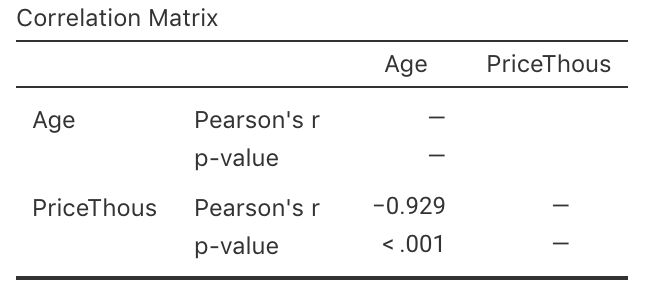
\includegraphics[width=0.57\linewidth]{SoftwareImages/Corollas-Correlation-jamovi} 

}

\caption{The jamovi correlation output, analysing the Corolla data.}\label{fig:CorollasPriceAgeCorrelationjamovi}
\end{figure}
\begin{figure}[hbtp]

{\centering 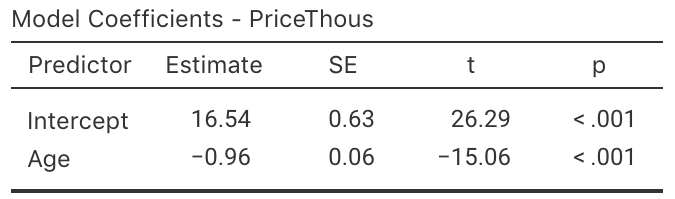
\includegraphics[width=0.6\linewidth]{SoftwareImages/Corollas-Regression-jamovi} 

}

\caption{The jamovi regression output, analysing the Corolla data.}\label{fig:CorollasPriceAgeRegressionjamovi}
\end{figure}

\begin{figure}[hbtp]

{\centering 
\includegraphics[width=0.6\linewidth]{12-TW12-Tutorial_files/figure-latex/CorollasPriceYear-1} 

}

\caption{The price of second-hand Toyota Corollas as advertised on Gum Tree on 25 June 2014 plotted against the year of manufacture ($n = 38$).}\label{fig:CorollasPriceYear}
\end{figure}

\section{Regression and correlation}\label{RegressionCorrelation}

Draw the regression line corresponding to \(\hat{y} = 5 + 2x\) for values of \(x\) between~\(0\) and~\(10\).

\begin{enumerate}
\def\labelenumi{\arabic{enumi}.}
\tightlist
\item
  Add some points to the scatterplot such that the correlation is approximately \(r = 0.9\).
  \answerbox{5}
\item
  Add some more points to the scatterplot such that the correlation is approximately \(r = 0.3\).
  \answerbox{5}
\end{enumerate}

\appendix \addcontentsline{toc}{chapter}{\appendixname}


\chapter{Answers for exercises}\label{OptionalAnswers}

This Appendix contains answers to \emph{most} (not all) exercises.
Some are fully worked, and some are only brief solutions.

\begin{itemize}
\tightlist
\item
  Answers for Tutorial~\ref{Lecture1} (Teaching Week~1): Sect.~\ref{Lecture1Answers}.
\item
  Answers for Tutorial~\ref{Lecture2} (Teaching Week~2): Sect.~\ref{Lecture2Answers}.
\item
  Answers for Tutorial~\ref{Lecture3} (Teaching Week~3): Sect.~\ref{Lecture3Answers}.
\item
  Answers for Tutorial~\ref{Lecture4} (Teaching Week~4): Sect.~\ref{Lecture4Answers}.
\item
  Answers for Tutorial~\ref{Lecture5} (Teaching Week~5): Sect.~\ref{Lecture5Answers}.
\item
  Answers for Tutorial~\ref{Lecture6} (Teaching Week~6): Sect.~\ref{Lecture6Answers}.
\item
  Answers for Tutorial~\ref{Lecture7} (Teaching Week~7): Sect.~\ref{Lecture7Answers}.
\item
  Answers for Tutorial~\ref{Lecture8} (Teaching Week~8): Sect.~\ref{Lecture8Answers}.
\item
  Answers for Tutorial~\ref{Lecture9} (Teaching Week~9): Sect.~\ref{Lecture9Answers}.
\item
  Answers for Tutorial~\ref{Lecture10} (Teaching Week~10): Sect.~\ref{Lecture10Answers}.
\item
  Answers for Tutorial~\ref{Lecture11} (Teaching Week~11): Sect.~\ref{Lecture11Answers}.
\item
  Answers for Tutorial~\ref{Lecture12} (Teaching Week~12): Sect.~\ref{Lecture12Answers}.
\end{itemize}

\begin{footnotesize}

\section{Answers for TW 1 tutorial}\label{Lecture1Answers}

\subsection*{Answers for Sect.~\ref{ResearchProcess}}\label{answers-for-sect.-refresearchprocess}

\textbf{Ask} the question.
\textbf{Design} the study.
\textbf{Collect} the data.
\textbf{Classify} and \textbf{summarize} the data.
\textbf{Analyse} the data.
\textbf{Report} the results.

\subsection*{Answers for Sect.~\ref{FormingRQs}}\label{answers-for-sect.-refformingrqs}

\begin{enumerate}
\def\labelenumi{\arabic{enumi}.}
\tightlist
\item
  \emph{Neither RQ is actually helping answer the issue of the café owner!}
  For example, I may be able to tell the difference between diet and regular cola\ldots{} but I may like them both equally (i.e., the taste rating is the same).
\item
  One option: For my customers, what proportion can distinguish diet and regular colas?
  P: The customers.
  O: The proportion that can distinguish regular ad diet colas.
  C: None.
  I: NO.
\item
  Many options: give a randomly-select cola (some regular; some diet), and record if customers can correctly identify it.
\end{enumerate}

\subsection*{Answers for Sect.~\ref{UnderstandingTerminology1}}\label{answers-for-sect.-refunderstandingterminology1}

You can use the \textbf{Glossary} in the textbook.

\subsection*{Answers for Sect.~\ref{UnderstandingTerminology2}}\label{answers-for-sect.-refunderstandingterminology2}

Answers implied by H5P.

\textbf{P}: People at an American college.
\textbf{O}: The \emph{average} time taken to walk \(50\)~m.
\textbf{C}: Between the way subjects were using their phone.
\textbf{I}: None: an observational study.

\textbf{Explanatory variable}: The way the phone is being used.
\textbf{Response variable}: The time taken to walk \(50\)~m.

\textbf{Unit of observation}: \emph{Individual} subjects.
\textbf{Unit of analysis}: \emph{Individual} subjects.

The purpose of taking data from every fifth individual: systematic sampling (on top of convenience sampling).
The purpose of taking data from individuals: people in groups often behave differently to individuals, and similarly to each other (for example: if one is talking to the others, the others are more likely to not be on their phone either).

\subsection*{Answers for Sect.~\ref{CreateRQs}}\label{answers-for-sect.-refcreaterqs}

\begin{enumerate}
\def\labelenumi{\arabic{enumi}.}
\item
  Many populations possible. The ``best'' population: the easiest, or cheapest to get?
  All of the options are possibilities.
\item
  ``Relaxing'': Many options possible for quantifying this (heart rate? breathing rate? survey? \emph{change} in heart rate before and after drinking the tea?).
\item
  Again, many options possible. Some options for comparing to Earl Grey tea: coffee; hot water; black tea; nothing at all; anything else but Early Grey; etc.
\item
  ``Between before and after drinking Earl Grey tea'' is \emph{not} a between-individuals comparison because everyone in the population (sample) is treated the same way: there are not two groups in the population being compared.
\item
  An example RQ might be:

  ``Among UniSC students (P), is the average heart rate \(30\)~mins after drinking (O) different between those who drink a cup of Earl Grey tea and those who drinking a cup of hot coffee (C) when the drink is provided to them (I)?''

  I'm not saying this is the best; it is just an example.
\item
  Get volunteers; place into one of the groups (Earl Grey and coffee); give the beverage; measure heart rate after \(30\)~mins.
  Note that many design issues are not covered until the next lecture.
\item
  An example RQ might be:

  ``Among UniSC students (P), is the average heart rate \(30\,\text{mins}\) after drinking (O) is different between those who drink a cup of Earl Grey tea and those who drinking a cup of hot coffee (C)?''
  I'm not saying this is the best; it is just an example.
\item
  Based on the above RQ: Find UniSC students who drink Earl Grey tea, and others who drink coffee, and measure their heart rate \(30\)~mins after they drink.

  It would have a lot of confounding effects to account for.
\item
  For my RQ above: The volume of tea or coffee; brand of tea or coffee; how made; when beverage taken; how long steeped for; how heart rate is measured; student (full-time only?); etc.
  You don't need to \emph{define} these, but if you have time you can have a go at one or two definitions.
\item
  Many options, but for the RQ above: type of beverage; heart rate after \(30\)~mins (or better, the \emph{change} in heart rate).
\end{enumerate}

\subsection*{Answers for Sect.~\ref{Units}}\label{answers-for-sect.-refunits}

\begin{enumerate}
\def\labelenumi{\arabic{enumi}.}
\tightlist
\item
  The unit of analysis is the \emph{floorboard}: because one board is compared to another; because the hardness is a feature of each board, not each test; because the two measurements on each board are not independent of each other (from the same board).
\item
  There are \(5\)~units of analysis.
\item
  There are \(10\)~units of observation.
\item
  Now, only one unit of analysis.
\item
  \emph{Within} boards, the variation is small, apart from Board~1.
  \emph{Between} boards it is larger.
\end{enumerate}

\subsection*{Answers for Sect.~\ref{TerminologyLect1}}\label{answers-for-sect.-refterminologylect1}

The answers, in alphabetical order, are: ask; analysis; analyse; collect; data; definitions; design; dingo; emu; estimation; evidence; joey; lurking; opal; POCI; qualitative; quantitative; relational; TAS; units.

\subsection*{Answers for Sect.~\ref{TypesOfStudies}}\label{answers-for-sect.-reftypesofstudies}

Answers implied by H5P.
Observational.
Quasi-experimental (the classes are determined by the \emph{students}, but the lecturer decides which class gets which treatment).

\section{Answers for TW 2 tutorial}\label{Lecture2Answers}

\subsection*{Answers for Sect.~\ref{StudyDesign}}\label{answers-for-sect.-refstudydesign}

\begin{enumerate}
\def\labelenumi{\arabic{enumi}.}
\tightlist
\item
  Read the \emph{Guidelines} carefully to find out!
\item
  The study is \emph{observational}, but because the researchers cannot determine the C (whether the person is a smoker or not).
  The critical element here is C, \emph{not} O.
\item
  This is a mix of both C (`smokers and non-smokers') and O (`the median serum cholesterol').
\item
  \emph{External validity} only refers to whether the \emph{sample} represents the given target \emph{population}, which is \emph{Australians}.
  Whether the results apply for the entire world is irrelevant.
\item
  ``Serum cholesterol'' is not a variable; nothing here is varying. ``Serum cholesterol'' is just a type of cholesterol.\\
  What actually varies--and so is the variable--is ``the serum cholesterol concentration'', or the ``value of serum cholesterol''.
\item
  This is \emph{not an experiment}, since the individuals cannot be directed into the comparison groups (between smokers and non-smokers) by the researchers.
\item
  In the data file, each row is a unit of analysis and each column is a variable.
  So there will be two variables but not those listed: one column will record the smoking status (Yes/No) and one column will record the serum cholesterol concentration.
\item
  A confounding variable has to be related to \emph{both} the response and explanatory variables.
\item
  The \emph{observer effect} is about how the \emph{researchers} might respond, \emph{not} the individuals under study.
\end{enumerate}

\subsection*{Answers for Sect.~\ref{LanguageReport}}\label{answers-for-sect.-reflanguagereport}

The answers are, in alphabetical order:
ACT; beach; blind; control; ethical; experimental; fire; gum; Hawthorne; help; MCG; nominal; randomly; relational; sample; three; treatment; Uluru.

\subsection*{Answers for Sect.~\ref{AssessReport}}\label{answers-for-sect.-refassessreport}

\begin{enumerate}
\def\labelenumi{\arabic{enumi}.}
\tightlist
\item
  \emph{Outcome}: average lifespan? Not sure how one measures `ageing well'. \tightlist
  \emph{Response variable}: lifespan?
\item
  \emph{Comparison}: Between eating and not eating aged cheese.
  \emph{Explanatory variable}: Whether someone eats aged cheese (or a certain amount of aged cheese) or not.
\item
  Observational; but a guess.
\item
  \emph{Outcome}: average lifespan; \emph{response}: lifespan.
\item
  \emph{Comparison}: Between mice drinking and not drinking spermidine; \emph{explanatory}: the type of water the mice drank.
\item
  Experimental; researchers treated the water.
\item
  Possibly; `aging well' is not the same as having an increased lifespan.
  Study is for \emph{mice}, not \emph{people} anyway.
\item
  To act as the control group, to measure the effect of the spermidine.
\item
  \emph{Outcome}: average blood pressure; \emph{response}: blood pressure.
\item
  Probably correlational, but possibly relational.
\item
  Observational.
\item
  Some answers are debatable.

  \begin{enumerate}
  \def\labelenumii{\alph{enumii}.}
  \tightlist
  \item
    Probably confounding (often is).
  \item
    Probably neither.
  \item
    Probably neither.
  \item
    Probably confounding.
  \item
    Probably extraneous.
  \end{enumerate}
\item
  Not really; but `ageing well' is very vague.
\item
  No; spermidine may have an effect, but probably not due to aged cheese intake.
\item
  No; observational.
\end{enumerate}

\subsection*{Answers for Sect.~\ref{StudyFeatures}}\label{answers-for-sect.-refstudyfeatures}

\begin{enumerate}
\def\labelenumi{\arabic{enumi}.}
\tightlist
\item
  Yes: `They were randomly allocated to take palmolein (``B9'') or canola (``T4'') crisps for the first 3 weeks, then (without a washout period) changed over to the other type, canola or palmolein for another 2 weeks'.
\item
  It has: `the type of oil was known only by the food scientist\ldots{}'
\item
  `the type of oil was known only by the food scientist\ldots{}'
\item
  Probably.
\item
  Subjects and researchers blinded.
\end{enumerate}

\section{Answers for TW 3 tutorial}\label{Lecture3Answers}

\subsection*{Answers for Sect.~\ref{StatsMode}}\label{answers-for-sect.-refstatsmode}

\begin{enumerate}
\def\labelenumi{\arabic{enumi}.}
\tightlist
\item
  Some of the significant figures look ridiculous.
  Mean: \(990.0791\), or \(990.1\)~tonnes.
  Standard deviation: \(1588.514579\), or \(1588.5\)~tonnes.
  (Specifically, \textbf{not} \(1485.919327\).)
\item
  Median: \(180.5\)~tonnes.
\item
  Splitting the data into two parts of four observations each:
  \(Q_1\) is half-way between \(8.0001\) and \(29.4\) tonnes: \(Q_1 = 18.7005\).
  \(Q_3\) is half-way between \(676.2\) and \(2547.3\) tonnes: \(Q_1 = 1611.75\).
  The IQR is \(1611.75 - 18.7005 = 1593.05\), or about \(1593\) tonnes.
\end{enumerate}

\subsection*{Answers for Sect.~\ref{UnderstandingVariation}}\label{answers-for-sect.-refunderstandingvariation}

Answers implied by H5P.
Median largest: \textbf{Class~D}.
Median smallest: \textbf{Class~C}.
Standard deviation largest: \textbf{Class~A}.
Standard deviation smallest: \textbf{Class~D}.

\subsection*{Answers for Sect.~\ref{UnderstandingHistograms}}\label{answers-for-sect.-refunderstandinghistograms}

Answers implied by H5P.

\begin{enumerate}
\def\labelenumi{\arabic{enumi}.}
\tightlist
\item
  Volume of drinks in \(375\,\text{mL}\): \textbf{Graph~D}.
  (Students sometimes say Graph~A, thinking that most cans have very similar amounts.)
\item
  Time in exam for \textbf{short} or \textbf{easy} exam: \textbf{Graph~C}.
\item
  Time in exam for \textbf{long} or \textbf{hard} exam: \textbf{Graph~B}.
\item
  The heights of females UniSC students: \textbf{Graph~D}.
\item
  The \emph{starting} salaries: \textbf{Graph~C}.
  (Students sometimes say Graph~B, thinking that salaries rise over time.)
\end{enumerate}

\subsection*{Answers for Sect.~\ref{InterpretingGraphs}}\label{answers-for-sect.-refinterpretinggraphs}

\begin{enumerate}
\def\labelenumi{\arabic{enumi}.}
\tightlist
\item
  Female Weddell: about \(260\)--\(270\,\text{cm}\) long, vary from about \(200\) to \(310\,\text{cm}\).
  Slight negative skewness; possible small outlier at about \(170\)--\(180\,\text{cm}\).
\item
  Dotchart.
  (Too much data for a useful stem-and-leaf plot probably.)
\item
  Better with a title; some more labelled tick marks would be better.
\item
  Part of this discussion can be about what information is needed on a publicity brochure.
\end{enumerate}

\subsection*{Answers for Sect.~\ref{Chapter3Drills}}\label{answers-for-sect.-refchapter3drills}

\begin{enumerate}
\def\labelenumi{\arabic{enumi}.}
\tightlist
\item
  Mean: \(168.5714\), or \(168.57\,\text{m}\).
  Standard deviation: \(6.966279\), or \(6.97\,\text{m}\).
  (Specifically, \textbf{not} \(6.44952\).)
  Median: \(167.9\,\text{m}\).
  IQR: \(175.0 - 162.5 = 12.5\,\text{m}\) (software may give a different value).
\item
  Descriptive.
  \(\bar{x} = 102.62\,\text{MPa}\); \(s = 5.356\,\text{MPa}\).
  The median is \(101.1\,\text{MPa}\).
\item
  Mean: \(13.88778\), or \(13.888\)\%.
  Standard deviation: \(2.617402\), or \(2.617\)\%.
  Median: \(13.35\)\%.
  IQR: \(16.115 - 11.66 = 4.455\)\% (software may give a different value).
\end{enumerate}

\subsection*{Answers for Sect.~\ref{CalculatorBatteries}}\label{answers-for-sect.-refcalculatorbatteries}

\begin{enumerate}
\def\labelenumi{\arabic{enumi}.}
\tightlist
\item
  Observational: the `treatment' (brand of battery) is not assigned; we simply take measurements from the batteries that exist.
\item
  Units of observation and units of analysis: The individual batteries.
\item
  \emph{Energizer}: mean: \(7.36\,\text{h}\); std dev: \(0.289\,\text{h}\).
  \emph{Ultracell}: mean: \(7.41\,\text{h}\); std dev: \(0.172\,\text{h}\).
\item
  Ultracell batteries are \emph{slightly} better (last longer) on average, and more consistent performers.
\item
  \emph{Energizer}: median: \(7.46\,\text{h}\).
  \emph{Ultracell}: median: \(7.48\,\text{h}\).
  So Ultracell batteries are \emph{slightly} better (last longer) on average.
\item
  Probably median (outliers?), but mean and median are similar in any case.
\item
  Values are close.\\
  Energizer batteries take, on average, \emph{less} time to reach \(1.0\) volts, so are `worse' in this regard.
  They also have a lot more variation.
  (Based on means, the difference is \(0.05\,\text{h}\), or \(3\,\text{mins}\) in over \(7\,\text{h}\) use!
  Based on medians, the difference is \(0.02\,\text{h}\), or \(1.2\,\text{mins}\)!)
  \textbf{The \emph{practical} difference is negligible.}
\item
  At the time of the study, the Ultracell batteries were substantially cheaper, and hence much better value.
\end{enumerate}

\section{Answers for TW 4 tutorial}\label{Lecture4Answers}

\subsection*{Answers for Sect.~\ref{PercentOddsStroke}}\label{answers-for-sect.-refpercentoddsstroke}

\begin{enumerate}
\def\labelenumi{\arabic{enumi}.}
\tightlist
\item
  Because the gender of the person is the explanatory variable.
\item
  (No answer.)
\item
  \(43\div (43 + 67) \times 100 = 39.1\)\%.
\item
  \(39\div (97 + 39) \times 100 = 28.7\)\%.
\item
  \(43\div 67 = 0.642\).
\item
  \(39\div 97 = 0.402\).
\item
  \(0.642 \div 0.402 = 1.6\).
\item
  (No answer; see online.)
\end{enumerate}

\subsection*{Answers for Sect.~\ref{TwoWayTables}}\label{answers-for-sect.-reftwowaytables}

\begin{enumerate}
\def\labelenumi{\arabic{enumi}.}
\tightlist
\item
  Because `Number of concussions' is the response variable.
\item
  Type of student:nominal (with three levels).
  Number of concussions: \emph{ordinal} (with three levels).
\item
  \(45\div 240 = 18.75\)\% of all college students in the sample have received one concussion.
\item
  We cannot calculate this as we \textbf{do not} have a population; we only have a sample.
\item
  Not sure which is best; they do different things.
  I'd probably prefer~(c) (bottom left graph).
\item
  Odds (non-athlete receiving 2+ concussions) is \(21\div(81 - 21) = 21\div 60 = 0.35\).
  Non-athletes are \(0.35\) times as likely to receive two or more concussions than fewer than two.
  Or: For every \(100\) students with fewer than two concussions, there are \(35\) with two or more.
\item
  Odds (soccer player receiving 2+ concussions) is \(13\div(63 - 13) = 13\div 50 = 0.26\).
  Soccer players are \(0.26\) times more likely to receive two or more concussions than fewer than two concussions.
\item
  OR: \(0.35 \div 0.26\), or about \(1.35\).
  The odds of a non-athlete receiving two or more concussions is about \(1.35\) times the odds of a soccer player receiving two or more concussions (that is, smaller odds for soccer players).
\item
  Not given.
\item
  Not given.
\item
  The better table is probably row percentages: the percentages of each type of students with given number of concussions.
\end{enumerate}

\subsection*{Answers for Sect.~\ref{WorkingWithOdds}}\label{answers-for-sect.-refworkingwithodds}

\begin{enumerate}
\def\labelenumi{\arabic{enumi}.}
\tightlist
\item
  The \emph{percentage} of bridges collapsing due to deterioration is \emph{36} divided by \emph{433}, or \(8.3\)\%.
\item
  The \emph{odds} of a bridge collapsing due to deterioration is \emph{36} divided by \emph{397}, or \(0.091\).
\item
  The odds of a bridge collapsing due to deterioration is \(0.091\); this means: \emph{b. For every \(100\) bridges that do not collapse due to deterioration, about \(9.1\) bridges do collapse}.
\item
  The percentage of bridges \emph{not} collapsing due to deterioration is \emph{397} divided by \emph{433}, or \(91.7\)\%.
\item
  The odds of a bridge \emph{not} collapsing due to deterioration is \emph{397} divided by \emph{36}, or \(11.0\).
\item
  The percentage of bridge collapses due to collisions is \emph{82} divided by \emph{433}, or \(18.9\)\%.
\item
  The odds of a bridge collapsing due to collisions is \emph{82} divided by \emph{351}, or \(0.234\).
\item
  The odds of an event cannot be larger than one: \emph{FALSE}.
\item
  The odds of an event cannot be smaller than one. \emph{FALSE}.
\item
  The following statement is true: \emph{c.~Odds cannot be negative}
\end{enumerate}

\subsection*{Answers for Sect.~\ref{Chapter4Drills}}\label{answers-for-sect.-refchapter4drills}

\begin{enumerate}
\def\labelenumi{\arabic{enumi}.}
\tightlist
\item
  \begin{enumerate}
  \def\labelenumii{\alph{enumii}.}
  \tightlist
  \item
    \((381 + 345)/1347 = 0.53898\), or about \(53.9\)\%.
  \item
    \((381 + 345)/(295 + 326) = 1.1691\), or about \(1.17\).
  \item
    \(345/326 = 1.05828\), or about \(1.06\).
  \item
    \(381/295 = 1.29153\), or about \(1.29\).
  \item
    \(1.05828 / 1.29153 = 0.81940\), or about \(0.819\).
  \end{enumerate}
\item
  \begin{enumerate}
  \def\labelenumii{\alph{enumii}.}
  \tightlist
  \item
    \((240 + 138)/960 = 0.39375\), or \(39.4\)\%.
  \item
    \((240 + 342)/960 = 0.60625\), or \(60.6\)\%.
  \item
    \((240 + 240)/960 = 0.5000\), or \(50\)\%.
  \item
    \((240 + 138)/(240 + 342) = 0.64948\), or about \(0.649\).
  \item
    \(240/240 = 1.000\).
  \item
    \(138/342 = 0.40351\) or about \(0.404\).
  \item
    \(0.40351/ 1.000 = 0.40351\) (i.e., the answer to f divided by the answer to e).
  \end{enumerate}
\end{enumerate}

\subsection*{Answers for Sect.~\ref{OddsRatioSMND}}\label{answers-for-sect.-refoddsratiosmnd}

\begin{enumerate}
\def\labelenumi{\arabic{enumi}.}
\tightlist
\item
  Backwards.
\item
  See Table~\ref{tab:SMNDAnswerTable}.
\item
  \(60/320 = 0.1875\).
  A worker with SMND is \(0.1875\) times as likely to have worked with metal than not.
\item
  \(33/344 = 0.096\).\\
  A worker without SMND is \(0.096\) times as likely to worked with metals than to have not worked with metals.
\end{enumerate}

\begin{table}
\centering
\caption{\label{tab:SMNDAnswerTable}SMND cases, and whether they had worked with metals.}
\centering
\fontsize{8}{10}\selectfont
\begin{tabular}[t]{lrrr}
\toprule
\textbf{ } & \textbf{Worked with metals} & \textbf{Did not work with metals} & \textbf{Total}\\
\midrule
SMND cases & 60 & 320 & 380\\
Controls & 33 & 344 & 377\\
Total & 93 & 664 & 757\\
\bottomrule
\end{tabular}
\end{table}

\section{Answers for TW 5 tutorial}\label{Lecture5Answers}

\subsection*{Answers for Sect.~\ref{CritiqueStudentSummaries}}\label{answers-for-sect.-refcritiquestudentsummaries}

\begin{enumerate}
\def\labelenumi{\arabic{enumi}.}
\tightlist
\item
  A few issues:
  Five decimal places is to the nearest \(0.01\) of a mm!
  The standard deviation of the difference is \emph{not} the difference between the individual standard deviations.
  A standard deviation cannot be negative. (Same applies to standard errors, but we aren't there yet.)
  Note that there is a sample size of~\(0\) for the difference!
\item
  The RQ is about a \emph{discrepancy} in proportions, or \emph{odds}, but these are not present in the table.
\end{enumerate}

\subsection*{Answers for Sect.~\ref{CritiqueStudentGraphs1}}\label{answers-for-sect.-refcritiquestudentgraphs1}

\begin{enumerate}
\def\labelenumi{\arabic{enumi}.}
\tightlist
\item
  A few issues: vertical axis is not labelled (presumably burn time in seconds); horizontal axis is not labelled (we have no way of knowing what is happening there.)
  \textless!--
\item
  A few issues: this is not a \emph{summary}: this shows the burn-time of every individual candle, and makes it hard to compare \emph{means} (which is the RQ); why is every bar labelled, which just adds unnecessary clutter; fonts are hard too read (small); a boxplot (or dotchart) would be the appropriate graph.
  In addition: the largest value is over \(70\,\text{mins}\)! Do a \emph{quick} project!
  --\textgreater{}
\item
  Reasonably good!
  The label on the vertical axis is a bit misleading: it is the \emph{number} of students; some wear grey-scale clothing and some do not.
\item
  A few issues: Compares just two numbers (means) using lots of ink; no indication of \emph{variation} in the data; a boxplot (or dotchart) would be appropriate.
\end{enumerate}

\subsection*{Answers for Sect.~\ref{UnderstandCorrelations}}\label{answers-for-sect.-refunderstandcorrelations}

\begin{enumerate}
\def\labelenumi{\arabic{enumi}.}
\tightlist
\item
  Correlation is inappropriate for \textbf{Plot~4} (non-linear) and \textbf{Plot~5} (non-linear).
\item
  \textbf{Plot~1}: \(0.94\) (correlation~\textbf{D});
  \textbf{Plot~2}: \(-0.95\) (correlation~\textbf{A});
  \textbf{Plot~3}: \(0.12\) (correlation~\textbf{B});
  \textbf{Plot~6}: \(0.75\) (correlation~\textbf{C}).
\item
  Examples of the direction in \textbf{Plot~1}: any two variables moderately positively correlated, such as height and weight, distance lived from university and travel time, etc.
\item
  Examples of direction in \textbf{Plot~2}: any two variables moderately negatively correlated, such as hours of weekly exercise and body weight, number of SCI110 tutorial missed and final mark, etc.
\item
  \textbf{Plot~1}: \(88.4\)\%;
  \textbf{Plot~2}: \(90.3\)\%;
  \textbf{Plot~3}: \(1.4\)\%;
  \textbf{Plot~6}: \(56.3\)\%.
\end{enumerate}

\subsection*{Answers for Sect.~\ref{WhichSummaryToUse}}\label{answers-for-sect.-refwhichsummarytouse}

Answers implied by H5P.

\begin{enumerate}
\def\labelenumi{\arabic{enumi}.}
\tightlist
\item
  Five variables. (`Participants' would not be summarised, it is technically an \emph{identifier} and \emph{not} a \emph{variable}, as each person has a unique value).
\item
  Age; Height; Weight and quantitative \textbf{continuous}.
\item
  Gender (\textbf{nominal}; two levels); GMFCS (\textbf{ordinal}; three levels)
\item
  As follows:

  \begin{itemize}
  \tightlist
  \item
    `Gender': Percentages (or number) F and M
  \item
    `Age': Mean/median; standard deviation/IQR
  \item
    `Height': Mean/median; standard deviation/IQR
  \item
    `Weight': Mean/median; standard deviation/IQR
  \item
    `GMFCS': Percentages (or numbers) in each group
  \end{itemize}
\item
  As follows:

  \begin{itemize}
  \tightlist
  \item
    `Gender': Barchart (not really needed)
  \item
    `Age': Histogram/stemplot
  \item
    `Height': Histogram/stemplot
  \item
    `Weight': Histogram/stemplot
  \item
    `GMFCS': Barchart/piechart
  \end{itemize}
\item
  As follows:

  \begin{itemize}
  \tightlist
  \item
    Between Gender and Height: Boxplot
  \item
    Between Gender and GMFCS: Side-by-side or stacked bar chart.
  \end{itemize}
\end{enumerate}

\section{Answers for TW 6 tutorial}\label{Lecture6Answers}

\subsection*{Answers for Sect.~\ref{NormalIQs}}\label{answers-for-sect.-refnormaliqs}

\begin{enumerate}
\def\labelenumi{\arabic{enumi}.}
\tightlist
\item
  (No picture).
\item
  \(130 - 100 = 30\) points above the mean.
\item
  Two standard deviations above the mean.
\item
  (No picture.)
\item
  \(-15\); that is, \(15\) IQ points \emph{below} the mean.
\item
  \(z = -1\); that is, one standard deviation \emph{below} the mean.
\item
  About \(84\)\%.
\end{enumerate}

\subsection*{Answers for Sect.~\ref{NormalHeights}}\label{answers-for-sect.-refnormalheights}

\begin{enumerate}
\def\labelenumi{\arabic{enumi}.}
\tightlist
\item
  Answers vary.
\item
  Answers vary.
\item
  Answers vary.
\item
  Answers vary.
  You probably cannot be very accurate using the \(68\)--\(95\)--\(99.7\) rule.
\item
  Answers vary.
\item
  Two standard deviations from the mean is \(2\times 6.7 = 13.4\), so \(95\)\% of females aged \(18\) and over have a measured height
  between \(161.4 \pm13.4\) approximately, or from \(148.0\)cm to \(174.8\)cm.
\item
  As follows:

  \begin{itemize}
  \tightlist
  \item
    \(z = (171 - 161.4)/6.7 = 1.43\), so the probability is \(0.9236\) or about \(92\)\%.
  \item
    So the odds are \(92.36/(100 - 92.36) = 12.1\).
  \item
    The answer is just \(1 - 0.9236 = 0.0764\) or about \(7.6\)\%.
  \item
    The probability of \textbf{over 171cm} is \(7.64\)\%.
  \item
    So the odds are \(7.64/(100 - 7.64)= 0.083\).
  \item
    \(z\)-scores are \(1.28\) and \(2.78\), so the answer is \(0.9973 - 0.8997 = 0.0976\), or about \(9.8\)\%.
  \item
    So the odds are \(9.8/(100 - 9.8) = 0.11\).
  \end{itemize}
\item
  Use the Tables: \(z = -0.84\); then using unstandardising formula, the height is \(x = \mu + (z\times\sigma) = 161.4 + (-0.84\times6.7) = 155.772\), or about \(156\,\text{cm}\).
\end{enumerate}

\subsection*{Answers for Sect.~\ref{Probability2}}\label{answers-for-sect.-refprobability2}

Answers embedded:
relative frequency;
relative frequency;
subjective;
relative frequency;
classical.

\subsection*{Answers for Sect.~\ref{RandomCardDraws}}\label{answers-for-sect.-refrandomcarddraws}

\begin{enumerate}
\def\labelenumi{\arabic{enumi}.}
\tightlist
\item
  Depends on data.
\item
  Looking close to normal, centred around \(0.5\)-ish.
\item
  We'd have an approximate normal distribution with mean \(\mu_{\hat{p}} = 0.5\) and standard deviation \(\text{s.e.}(\hat{p}) = \sqrt{0.5 \times (1 - 0.5)/10} \approx 0.158\).
\item
  Still normal; same mean; but standard deviation would be smaller: \(\text{s.e.}(\hat{p}) = \sqrt{0.5 \times (1 - 0.5)/50} \approx 0.071\).
\end{enumerate}

\subsection*{Answers for Sect.~\ref{NormalSOI}}\label{answers-for-sect.-refnormalsoi}

\begin{enumerate}
\def\labelenumi{\arabic{enumi}.}
\setcounter{enumi}{1}
\tightlist
\item
  \(z = (20 - 0)/10 = 2\).
  The area or probability to the \emph{right} is \(0.0228\), or about \(2.3\)\%.
\item
  The probability the SOI exceeds \(20\): \(2.3\)\%.
  So odds: \(2.3\div(100 - 2.3)\), or about \(0.024\).
\item
  \(z = (-25 - 0)/10 = -2.5\).
  The area to the \emph{left} is \(0.0062\), or about \(0.6\)\%.
\item
  \(z = (-12 - 0)/10 = -1.2\).
  The area to the \emph{right} is \(0.8849\), or about \(88.5\)\%.
\item
  The two \(z\)-scores: \((-10 - 0)/10 = -1\) and \((20 - 0)/10 = 2\).
  The area \emph{between} these is \(0.9772 - 0.1587 = 0.8185\), or about \(81.9\)\%.
\item
  The \(z\) score corresponds to an area of \(0.80\) to the \emph{left}; from the tables, about \(z = 0.84\).
  This corresponds to an SOI of \(0 + (0.84\times 10)\), or an SOI of about \(8.4\).
\item
  The \(z\)-score is \(0.385\) from Appendix~3 in the textbook, remembering that the area to the \emph{left} would be \(0.650\) (draw a diagram!).
  So, the \(z\)-score is \(0.385\), so that the SOI values is \(x = \mu + (z\times\sigma) = 0 + (0.385\times 10) = 3.85\).
\item
  \(z = -4.5\); from a picture of the normal distribution, the probability that \(z\) is greater than \(-4.5\) is practically (but not exactly) \(100\)\%: the SOI is practically \emph{always} larger than~\(55\).
\item
  Draw a picture of a normal distribution: half the SOI values are bigger than~\(0\), and half are smaller than~\(0\).
\end{enumerate}

\section{Answers for TW 7 tutorial}\label{Lecture7Answers}

\subsection*{Answers for Sect.~\ref{ConceptsMatches}}\label{answers-for-sect.-refconceptsmatches}

\begin{enumerate}
\def\labelenumi{\arabic{enumi}.}
\item
  This is just one box of matches (one \emph{observation}), but the claim is about the \emph{population mean}.
  Some boxes will have more than \(45\), and some fewer.
\item
  Jake is correct in one sense: You can't have \(0.9\) of a match.
  But the value is the \emph{mean} number, and that \emph{can} be a decimal.
  Suppose \(10\) boxes had \(49\) matches, and \(10\) boxes had \(50\) matches\ldots{} is the mean \(49\), or is it \(50\)?
  Neither are correct; the mean is \(49.5\).
\item
  Jake is confusing the \emph{sample} and \emph{population} mean.
  The claim is that the \emph{population} mean is \(45\).
  The sample produced a mean of \(44.9\).

  Why should the mean of two different things be the same?
  It's like expecting your height and your Mum's height to be the same:
  they are both heights, but of different things.
  Why should they be the same?

  Of course, every sample will produce a different sample mean.
  This sample may just have an unusually low number of matches.
\item
  Either (1)~The manufacturer is lying; or (2)~the manufacturer is \emph{not} lying, and this sample just happens to have a smaller number of matches: (bad) luck.
\item
  A CI gives some indication of the variation implied by the sample.
\item
  Probably around \(0.4\)~matches.
  (Three standard deviations either side of the mean would be about \(0.4 \times 3 = 1.2\) ~matches either side of the \(45\)~target, much more reasonable than any other option.)
\item
  The standard error for the mean is \(0.124\div\sqrt{25} = 0.0248\).
  So the approximate \(95\)\%~CI is: \(44.9 \pm (2\times 0.0248)\), or \(44.9\pm 0.0496\), or from \(44.85\) to \(44.95\).
\item
  No.~A \(95\)\% CI may or may not contain the population mean.
  Of course, the manufacturer \emph{may} indeed be lying\ldots{}
  but we'd need to be cautious about making such a bold claim on just this evidence.
  Ideally, we would repeat this study a few times or take a larger sample.
  But it \emph{is} looking suspicious\ldots{}

  If we had many, many sets of \(25\)~matches boxes,
  \(95\)\% of these sets of~\(25\) would have a mean between \(44.85\) and \(44.95\).
\item
  \(\bar{x}\) is the mean of the sample, so \(\bar{x} = 44.9\).
\item
  \(\mu\) is the mean of the population; the true mean if you like.
  \(\mu\) is \emph{claimed} to be \(45\), but the the value of \(\bar{x}\) will, of course, vary.
\end{enumerate}

\subsection*{Answers for Sect.~\ref{SEproportions}}\label{answers-for-sect.-refseproportions}

Answers implied by H5P.

\(\displaystyle \text{s.e.}(\hat{p}) = \sqrt{ \big(\hat{p}\times(1 - \hat{p}) \big)/n}\), where \(\hat{p}\) is the \emph{sample proportion}; \(n\) the \emph{sample size}; ``s.e.'' the ``standard error''.

\subsection*{Answers for Sect.~\ref{CIPropBVM}}\label{answers-for-sect.-refcipropbvm}

\begin{enumerate}
\def\labelenumi{\arabic{enumi}.}
\tightlist
\item
  \(123/(404 - 123) = 123/281 = 0.44\).\tightlist
\item
  \(\hat{p} = 123/404 = 0.304455\).
\item
  The \textbf{odds}: The likelihood of surviving is about \(0.44\) times the probability of dying (i.e., it is lower).
  Or: For every \(100\) that die, about \(44\) survive.
  The \textbf{proportion}: About~\(30.4\) of every~\(100\) patients survive.
\item
  No: sampling variation!
\item
  \(\text{s.e.}(\hat{p}) = \sqrt{0.304455 \times (1 - 0.304455)/404} = \sqrt{0.00052416} = 0.022894\), or about \(0.023\).\\
  A definition can be found in the textbook \emph{Glossary}.
  Essentially, each sample is likely to produce a different value for the sample proportion, \(\hat{p}\) (the estimate of the population proportion, \(p\)), and that is what we mean by ``sampling variation''.
\item
  (Not provided.)
\item
  The values of \(\hat{p}\) will have an approximate normal distribution, with a standard deviation equal to standard error (\(0.023\)) and centred around the true proportion \(p\).
  A \(95\)\% CI: \(0.304455 \pm (2\times0.022894)\), or \(0.30446\pm0.04579\), or \(0.26\) to \(0.35\).
\item
  One way of writing communicating: ``The population proportion of patients surviving after BVM treatment has a \(95\)\% chance of lying between \(26\)\% and \(35\)\%.''
  This is not strictly correct, but acceptable and very, very commonly used (as explained in the textbook.
\item
  Larger, to get a tighter (more precise) CI than the one calculated.
\item
  The number of surviving and non surviving both exceed \(5\).
\end{enumerate}

\subsection*{Answers for Sect.~\ref{CIPizzas}}\label{answers-for-sect.-refcipizzas}

\begin{enumerate}
\def\labelenumi{\arabic{enumi}.}
\tightlist
\item
  \(\mu\) is the population mean diameter size of \emph{all} EB pizzas;
  \(\bar{x}\) is the mean diameter of the pizzas in the sample.
\item
  \(\bar{x} = 11.486\) inches; it's not sensible to quote the diameter to \(0.001\) of an inch; what \emph{would} be is sensible?
  We don't know the value of \(\mu\), and we never will.
  Our best \emph{estimate} is the value of \(\bar{x}\).
\item
  \(s = 0.24658\) inches.
  It's not sensible to quote the diameter to \(0.001\) of a cm though.
  \(\sigma\) is the standard deviation of the population.
  We don't know the value of \(\sigma\), and we never will.
\item
  \(\displaystyle\text{s.e.}(\bar{x}) = s/\sqrt{n} = 0.24658/\sqrt{125} = 0.02205\).
\item
  The first measures the variation in the diameters of individual pizzas; the second measures the precision of the sample mean when used to estimate the population mean.
\item
  Almost certainly not the same.
  Probably close to \(\bar{x} = 11.486\) inches.
  More precisely, probably within three standard errors (\(3\times 0.022\)) of \(\bar{x}\).
\item
  Normal; mean \(\mu\); std. dev is the standard error of \(0.02205\).
\item
  The approximate \(95\)\% CI is \(11.486\pm (2\times 0.02205)\) or \(11.486\pm0.044\), which is from \(11.44\) to \(11.53\) inches.
\item
  Based on the sample, a \(95\)\% confidence interval for the population mean for the pizza diameter is between \(11.44\) and \(11.53\) inches.
\item
  \(n > 25\) \textbf{or} \(n\le 25\) and population has normal distribution.
\item
  We do not need to \textbf{assume} that \(n > 25\) because we know that it is.
  We do \emph{not} require that the sample or the population has a normal distribution.
  We require that the \emph{sample means} have an approximate normal distribution, which they will if \(n > 25\).
  So the CI is statistically valid, and the histogram is not needed.
\item
  Population mean diameter probably not \(12\) inches based on the CI.
\end{enumerate}

\subsection*{Answers for Sect.~\ref{Chapter6Drills}}\label{answers-for-sect.-refchapter6drills}

\begin{enumerate}
\def\labelenumi{\arabic{enumi}.}
\tightlist
\item
  \(\sqrt{0.70\times(1 - 0.70)/25} = \sqrt{0.0084} = 0.09165151\), or about \(0.09165\).
\item
  \(\sqrt{0.25\times(1 - 0.25)/100} = \sqrt{0.001875} = 0.04330127\), or about \(0.04330\).
\item
  \(0.08724964\), or about \(0.08725\).
\item
  \(0.0534479\), or about \(0.05345\).
\end{enumerate}

All statistically valid.

\textbf{Note}: Students commonly forget to take the square root.

\textbf{Note}: If you calculator gives an answer something like \texttt{1.875\ E-03} or similar, it is using \textbf{scientific notation}.
It means \(1.875\times 10^{-3}\), or \(0.001875\).

\section{Answers for TW 8 tutorial}\label{Lecture8Answers}

\subsection*{Answers for Sect.~\ref{HTOneProportionA}}\label{answers-for-sect.-refhtoneproportiona}

\begin{enumerate}
\def\labelenumi{\arabic{enumi}.}
\tightlist
\item
  \(H_0\): \(p = 0.3\) and \(H_1\): \(p > 0.3\).
\item
  \(\hat{p} = 12/35 = 0.3428571\).
\item
  \(\text{s.e.}(\hat{p})
  = \sqrt{0.3 \times 0.7/35} = 0.07745967\).
  (Make sure to use \(p\) not \(\hat{p}\) in the standard error calculation for the test!)
\item
  \(z = (0.3428571 - 0.3)/0.07745967 = 0.553\).
\item
  The \(z\)-value is very small---less than one standard deviation from the mean---so the \(P\)-value will be quite large:
  `The data present no evidence (\(z = 0.55\); \(P > 0.05\)) that computer programmers are more likely to wear contact lenses (\(\hat{p} = 0.342\); approx. \(95\)\% CI from \(0.182\) to \(0.503\)).'
  (For the CI, remember to use \(\hat{p}\) in the standard error calculation: \(\text{s.e.}(\hat{p}) = 0.0802329\).)
\item
  For \emph{statistical validity}, we require that the number of people \emph{with} and \emph{without} contact lenses to be at least~\(5\), which is true (\(12\) and \(23\) respectively).
  For \emph{external validity}, the sample must be a random sample of Swedish programmers.
\end{enumerate}

\subsection*{Answers for Sect.~\ref{HTOneMean-A}}\label{answers-for-sect.-refhtonemean-a}

\begin{enumerate}
\def\labelenumi{\arabic{enumi}.}
\item
  The \textbf{parameter} of interest is the \emph{population mean pizza diameter}, say \(\mu\).\tightlist
\item
  From the output: \(\bar{x} = 11.486\)~inches and \(s = 0.247\)~inches.
\item
  Use \(\text{s.e.}(\bar{x}) = s/\sqrt{n} = 0.247/\sqrt{125} = 0.02205479\)~inches.
\item
  \(s\) tells us the variation in diameter from pizza to pizza.
  \(\text{s.e.}(\bar{x})\) tells us how much the sample mean is likely to vary from sample to sample, in sample of size~\(125\).
\item
  The hypotheses are:

  \(H_0\): The mean diameter is \(12\) inches; or \(\mu = 12\).\\
  \(H_1\): The mean diameter is not \(12\) inches; or \(\mu \ne 12\)
\item
  Two-tailed, because the RQ asks if the diameter is \(12\) inches, or not.
\item
  The normal distribution has a mean of \(12\), and a standard deviation of \(\text{s.e.}(\bar{x}) = 0.022092\).
\item
  \(t = (11.486-12)/0.022092 = -23.3\).
\item
  The \(t\)-score is \emph{huge} (and negative), so the \(P\)-value is \emph{very} small.
  (Two-tailed \(P<0.001\) from the table or from software.)
\item
  Very strong evidence exists in the sample (\(t = -23.3\)\$; two-tailed \(P\) less than \(0.001\)) that the population mean pizza diameter of pizzas from Eagle Boys' is less than \(12\) inches (sample mean diameter: \(11.49\) inches; std. dev.: \(0.246\);
  \(95\)\% CI from \(11.44\) to \(11.53\) inches; approximate 95\% CI is \(11.486\pm 0.0441\)).
\item
  Since \(n\) is much larger than \(25\), we do not require that the population has a normal distribution, just that the population is not grossly non-normal; the sample means will still have an approximate normal distribution.
\item
  \emph{Very} unlikely!
\end{enumerate}

\subsection*{Answers for Sect.~\ref{PValues}}\label{answers-for-sect.-refpvalues}

Use the \(68\)--\(95\)--\(99.7\) rule to \emph{approximate} the \(P\)-values:
\emph{Less than} \(0.05\); Greater than \(0.05\);
\emph{Less than} \(0.003\);
Greater than \(0.05\);
Greater than \(0.05\);
Very small.

\subsection*{Answers for Sect.~\ref{HtestWritingConclusions}}\label{answers-for-sect.-refhtestwritingconclusions}

\begin{enumerate}
\def\labelenumi{\arabic{enumi}.}
\tightlist
\item
  \emph{Correct}: \(H_1\): \(p \ne 0.40\) (i.e., the population proportion of students using AI daily is \textbf{not}~\(0.40\), the claim).

  \begin{enumerate}
  \def\labelenumii{\alph{enumii}.}
  \tightlist
  \item
    `Significant' is not appropriate in the hypothesis.
  \item
    No parameter is given; the hypothesis should include (and define!) the parameter~\(p\), the proportion of students using AI daily.
  \item
    The alternative is \emph{not equal to} \(0.40\).
  \item
    The hypothesis are \textbf{not} about the \emph{numbers}; they are about \emph{proportions}.
  \end{enumerate}
\item
  \(P\) is big much larger than \(0.05\).
\item
  \emph{Correct}: There is no evidence that the population proportion of students using AI daily is not~\(0.40\), as claimed.

  \begin{enumerate}
  \def\labelenumii{\alph{enumii}.}
  \tightlist
  \item
    `No \textbf{strong}' evidence' is wrong: there is `no evidence'.
  \item
    `No evidence of a \textbf{large} difference' is wrong: there is no evidence of a difference.
  \item
    The sample proportion is \(\hat{p} = 29/78 = 0.372\), so this is clearly \textbf{wrong}!
  \end{enumerate}
\item
  \(P\) is a bit smaller than \(0.05\).
\item
  \emph{Correct}: There is evidence that the population proportion of students using AI daily is not~\(0.40\)\%.

  \begin{enumerate}
  \def\labelenumii{\alph{enumii}.}
  \tightlist
  \item
    `There is evidence of a \textbf{significant} difference': the use of `significant' here is incorrect.
  \item
    This is not true: we start by assuming the claim is true; we don't need the evidence to support it.
    There is evidence, however, to support the alternative hypothesis.
  \item
    The claimed proportion is stated as being \(0.40\), so this is clearly \textbf{wrong}!
  \end{enumerate}
\end{enumerate}

\subsection*{Answers for Sect.~\ref{DecisionMakingProcess}}\label{answers-for-sect.-refdecisionmakingprocess}

Answers implied by H5P.

\begin{enumerate}
\def\labelenumi{\arabic{enumi}.}
\tightlist
\item
  The decision-making process begins with making an assumption about the population \textbf{parameter}.
  This means we know what to \textbf{expect} from the sample \textbf{statistic}. We never know exactly what value of the statistic we will see in the sample, because of \textbf{sampling variation}.
  But we can have some of idea of what values are reasonable to expect.
  Then we take the \textbf{sample} (that is, we make the observations).
  Then we \textbf{compare} the sample statistic that we observed\ldots{} to the sample statistic we expected.
  If what we observe is inconsistent with what was expected, then the the assumption is \textbf{unlikely to be} true.
  However, if what we observe is \textbf{consistent} with what was expected, then the the assumption is \textbf{probably} true.
\end{enumerate}

\section{Answers for TW 9 tutorial}\label{Lecture9Answers}

\subsection*{Answers for Sect.~\ref{MatchRQHypothesis}}\label{answers-for-sect.-refmatchrqhypothesis}

Answers implied by H5P.

\emph{Null} hypotheses:

\begin{enumerate}
\def\labelenumi{\arabic{enumi}.}
\tightlist
\item
  Is the mean length of a \(12\)-inch sub really \(12\) inches?
  \textbf{F}: \(\mu = 12\).
\item
  Is the mean length of a \(12\)-inch sub different for white and wholemeal subs?
  \textbf{B}: \(\mu_{\text{white}} - \mu_{\text{wholemeal}} = 0\).
\item
  Is the proportion of \(12\)-inch subs shorter than \(12\) inches different for white, wholemeal subs?
  \textbf{A}: \(p_{\text{white}} - p_{\text{wholemeal}} = 0\).
\item
  Is the mean length of a \(12\)-inch sub longer for white (compared to wholemeal) subs?
  \textbf{B}: \(\mu_{\text{white}} - \mu_{\text{wholemeal}} = 0\).
\end{enumerate}

\emph{Alternative} hypotheses:

\begin{enumerate}
\def\labelenumi{\arabic{enumi}.}
\tightlist
\item
  Is the mean length of a \(12\)-inch sub really \(12\) inches?
  \textbf{I}: \(\mu \ne 12\).
\item
  Is the mean length of a \(12\)-inch sub different for white and wholemeal subs?
  \textbf{G}: \(\mu_{\text{white}} - \mu_{\text{wholemeal}} \ne  0\).
\item
  Is the proportion of \(12\)-inch subs shorter than \(12\) inches different for white, wholemeal subs?
  \textbf{K}: \(p_{\text{white}} - p_{\text{wholemeal}}\ne 0\).
\item
  Is the mean length of a \(12\)-inch sub longer for white (compared to wholemeal) subs?
  \textbf{L}: \(\mu_{\text{white}} - \mu_{\text{wholemeal}} > 0\).
\end{enumerate}

\subsection*{Answers for Sect.~\ref{LimeTreesjamovi}}\label{answers-for-sect.-reflimetreesjamovi}

\begin{enumerate}
\def\labelenumi{\arabic{enumi}.}
\tightlist
\item
  Mean for natural trees (\(\mu_N\)), minus the mean for planted trees (\(\mu_P\)).
\item
  \(\mu_N - \mu_P\).
\item
  The difference between the population means could be between \(2.7\,\text{cm}\) larger for planted trees, to \(1.5\,\text{cm}\) larger for natural trees.
\item
  The difference between the population means could be between \(0.6\,\text{cm}\) and \(4.0\,\text{cm}\) larger for natural trees.
\item
  The difference between the population means could be between \(1.6\,\text{cm}\) and \(4.5\,\text{cm}\) larger for planted trees.
\end{enumerate}

\subsection*{Answers for Sect.~\ref{CIImplant}}\label{answers-for-sect.-refciimplant}

\begin{enumerate}
\def\labelenumi{\arabic{enumi}.}
\tightlist
\item
  How much further patients walk \emph{with} the implant.
\item
  Without minus With (i.e., How much further patients walk \emph{with} the implant).
\item
  \textbf{Repeated-measures}:
  Every subject has two TWMT recorded.
\item
  \(\mu_d\) is the mean difference in the target population; \(\bar{d}\) is the mean difference in this sample.
\item
  Each measurement is measured after and before on the same subject.
\item
  \(32\); \(12\); \(24\); \(30\); \(8\); \(14\); \(14\); \(28\); \(38\); \(49\).
  (Differences in the other direction are also acceptable; it just changes the signs of these differences and so on.
  \textbf{Importantly, the direction should be stated somewhere.})
\item
  It makes more sense to define directions this way, so that the difference is the \emph{increase} in 2MWT.
\item
  \(\bar{d} = 24.9\); \(s_d=13.03372\,\text{m}\).
\item
  \(\text{s.e.}(\bar{d}) = s_d/\sqrt{n} = 13.03372/\sqrt{10} = 4.121623\,\text{m}\).
\item
  This is the standard deviation of the sample mean difference, a measurement of how precisely the sample mean difference measures the population mean difference.
\item
  Almost impossible.
  Sample means vary every time we take a sample around the true mean difference, with a normal distribution with standard error \(4.12\).
  Since we don't know \(\mu\), the best we can say is that the sample mean will vary about our best guess of the population mean; in other words, the sample means vary around \(24.9\) with a standard deviation of about \(4.12\).
\item
  Normal; mean \(\mu_d\), std deviation is the standard error of \(4.121\).
\item
  \(24.9\pm (2\times 4.121623)\), or \(24.9\pm 8.243246\), or from \(16.65675\) to \(33.143245\,\text{m}\).
\item
  Only \emph{one sample of people} have been studied, so it is (as always) hard to be sure.
\item
  \(H_0\): \(\mu_d = 0\), differences defined as `with' minus `without'.
  \(H_1\): \(\mu_d > 0\) the way I defined differences.\\
\item
  \(t = 6.041\) and since \(t\) is very large, expect \(P\) to be very small.
\item
  The differences have just been defined in the opposite directions.
  (Notice the \(P\)-values are the same.)
\item
  Very strong evidence exists in the sample (paired \(t = 6.041\); one-tailed \(P\) less than \(0.0005\)) that the population mean 2MWT are higher after receiving the implant compared to without the implant (mean difference: \(24.9\,\text{m}\) higher after receiving the implant; standard deviation: \(13.034\,\text{m}\); \(95\)\%~CI from \(16.66\) to \(33.14\,\text{m}\)).
\item
  The population of differences has a normal distribution, and/or \(n > 25\) or so.
\item
  Since \(n < 25\), must assume the population of differences has a normal distribution.
  The histogram suggests this is not unreasonable.
\end{enumerate}

\subsection*{Answers for Sect.~\ref{CIRatLifetimes}}\label{answers-for-sect.-refciratlifetimes}

\begin{enumerate}
\def\labelenumi{\arabic{enumi}.}
\item
  The two groups are different rats. \tightlist
\item
  The \textbf{parameter} of interest is the \emph{difference between the population mean lifetimes}, say \(\mu_R - \mu_F\).
  Measure how much longer the lifetimes are for rats on a restricted diet.
\item
  Table not shown.
\item
  The \(95\)\%~CI is the \emph{bottom} one: from \(223.34\) to~\(346.13\)~days.
\item
  The best of these is Option~(e)\ldots{} but in practice, we usually think about CIs in terms of Option~(d) so Option~(d) is fine.
\item
  The CI explanation can be improved by (i)~indicating \emph{which} diet leads to larger average lifetimes; and (ii)~providing sample summary info. Here is a better answer:

  ``The \(95\)\% confidence interval for the difference between the populations mean lifetimes of rats on the restricted diet (sample mean: \(968.8\) days; std dev: \(284.6\) days) and on the free-eating diet (\(684.0\) days; std dev: \(134.1\) days) is that rats on a restricted diet live between \(223.34\) and \(346.13\) days longer.''
\item
  Boxplots: shows the variation in the lifetimes of individual rats.
  Error bar chart: displays the variation that the sample means would be expected to show from sample to sample.
\item
  The null hypothesis is that there is no difference in the mean lifetimes of the two groups of rats.
  In symbols (where \(\mu\) represents the mean lifetime in the population):

  \(H_0\): \(\mu_R = \mu_{FE}\); and \(H_1\): \(\mu_R > \mu_{FE}\); \textbf{one}-tailed, because of the RQ.
\item
  Either sampling variation explain the difference, or the diets really are different.
\item
  Use the not-equal variance (Welch's test) row: \(t = 9.161\); one-tailed \(P < 0.0005\) (test is one-tailed).
\item
  \(t = (284.73 - 0)/31.08 = 9.16\), as per output.
\item
  The evidence contradicts \(H_0\).
  Very strong evidence exists in the sample (\(t = 9.161\) for two independent samples; \(\text{df} = 154.94\); one-tailed \(P < 0.0005\)) that the population mean lifetime of rats on a restricted diet (mean lifetime: \(968.75\)~days; std. dev.: \(284.6\)~days) is greater than rats on a free-eating diet (\(684.01\)~days; \(134.1\)) (\(95\)\%~CI for the difference from \(223.3\) to~\(346.1\)~days).
\item
  The \emph{sample means} have a normal distribution.
  Since both sample sizes are greater than~\(25\), this is true.
  The figure suggests not very severe non-normality.
\item
  Rats from the same litter are likely to be similar to each other.
  The litter would probably be the unit of analysis then, not the individual rat.
\end{enumerate}

\subsection*{Answers for Sect.~\ref{JumpingInference}}\label{answers-for-sect.-refjumpinginference}

\(H_0\): \(\mu_d = 0\) and \(H_1\): \(\mu_d\ne 0\), where \(\mu_d\) is the mean difference (shoes minus barefoot, from the second table).
\(t = -2.231\); \(P = 0.029\).
Moderate evidence of a mean difference (approx. \(95\)\%~CI: \(0.066\) to~\(1.206\,\text{cm}\) greater barefoot).

\subsection*{Answers for Sect.~\ref{ReactionTimeInference}}\label{answers-for-sect.-refreactiontimeinference}

\(H_0\): \(\mu_P = \mu_N\) and \(H_1\): \(\mu_P\ne \mu_N\), where \(\mu_P\) is the mean reaction time \emph{with} a phone and \(\mu_N\) is the mean reaction time \emph{with no phone}.
Using summary table: \(t = (51.59 - 0)/19.612 = 2.63\), so \(P\)-value will be smaller than \(0.05\) (based on \(68\)--\(95\)--\(99.7\) rule).
Strong evidence of a difference between the mean reaction times; approx. \(95\)\%~CI: \(12.37\) to~\(90.81\,\text{s}\) slower (i.e., greater) with phone.

\section{Answers for TW 10 tutorial}\label{Lecture10Answers}

\subsection*{Answers for Sect.~\ref{Consistency}}\label{answers-for-sect.-refconsistency}

If the RQ is about odds (and hence odds ratios), then the hypothesis, CI and hypothesis tests should also be about odds.
(Similarly, if the RQ is about proportions, then the hypothesis, CI and hypothesis tests should also be about proportions.)

\begin{enumerate}
\def\labelenumi{\arabic{enumi}.}
\setcounter{enumi}{3}
\tightlist
\item
  From the output, the OR is \(0.508\).
\item
  The \emph{odds ratio} here means, from the RQ
  \[
    \text{OR} = \frac{\text{Odds of bites, using citronella candle}}{\text{Odds of bites, using wax candle}}.
  \]
\item
  The odds of someone receiving mosquito bites when sitting near a citronella candle is \(0.51\) times the odds for those sitting near a wax candle (i.e., is lower).
\item
  The difference between proportions is \(p_C- p_W\).
  In the population, the proportion of people bitten by mosquitoes is between \(0.344\) higher near a \textbf{wax} candle to \(0.024\) higher near a \textbf{citronella} candle.
\item
  \(0.51\times 2.167 = 1.1\).
\item
  In the population, the odds of someone receiving mosquito bites when sitting near a citronella candle is between \(0.234\) times (i.e., lower) and \(1.102\) times (i.e., higher) than the odds for those sitting near a wax candle.
\item
  In the population, the odds of someone receiving mosquito bites when sitting near a citronella candle is between \(0.11\) and \(0.94\) times the odds for those sitting near a wax candle (i.e., is lower).
  10.In the population, the odds of someone receiving mosquito bites when sitting near a citronella candle is between \(1.28\) and \(4.13\) times the odds for those sitting near a wax candle (i.e., is higher).
\item
  The smallest expected count will be \(42\times 44/118 = 15.7\), which comfortably exceeds five: the CIs are statistically valid.
\end{enumerate}

\subsection*{Answers for Sect.~\ref{OddsSoftware}}\label{answers-for-sect.-refoddssoftware}

\begin{enumerate}
\def\labelenumi{\arabic{enumi}.}
\tightlist
\item
  See Table~\ref{tab:MatTable}.
\item
  Side-by-side or stacked bar chart.
\item
  \(352/2512 = 0.1401\).
\item
  \(336/2328 = 0.1443\).
\item
  \(0.1401/0.1443 = 0.971\).
\item
  The odds ratio, of a boy maturing late compared to a girl maturing late.
\item
  OR: \(0.971\), with \(95\)\% CI from \(0.828\) to \(1.139\).
\item
  See Table~\ref{tab:MatNumSummary}.
\item
  \(P = 0.717\); no evidence of a difference between boys and girls.
\end{enumerate}

\begin{table}
\centering
\caption{\label{tab:MatTable}Maturation data table.}
\centering
\fontsize{8}{10}\selectfont
\begin{tabular}[t]{lrrr}
\toprule
\textbf{ } & \textbf{Late} & \textbf{Not late} & \textbf{Total}\\
\midrule
Males & 352 & 2512 & 2864\\
Females & 336 & 2328 & 2664\\
Total & 688 & 4840 & 5528\\
\bottomrule
\end{tabular}
\end{table}

\begin{table}
\centering
\caption{\label{tab:MatNumSummary}Numerical summary table for maturation data.}
\centering
\fontsize{8}{10}\selectfont
\begin{tabular}[t]{lrrr}
\toprule
\textbf{ } & \textbf{Prop late} & \textbf{Odds late} & \textbf{Sample size}\\
\midrule
Males & 0.123 & 0.1401 & 2864\\
Females & 0.126 & 0.1443 & 2664\\
\midrule\\
 & Diff: -0.003 & OR: 0.971 & \\
\bottomrule
\end{tabular}
\end{table}

\subsection*{Answers for Sect.~\ref{TestsForORs}}\label{answers-for-sect.-reftestsforors}

Some answers embedded.

\begin{enumerate}
\def\labelenumi{\arabic{enumi}.}
\item
  See Table~\ref{tab:ArtLimbMortalityANS}. \tightlist
\item
  Use of artificial limb is the explanatory variable.
\item
  Using artificial limb: \(49/16 = 3.0625\).
  Not using artificial limb: \(21/19 = 1.105263\).
  The OR is \(3.0625/1.105263 = 2.771\); that is, the odds of being alive after five years is almost three times higher for those using an artificial limb compared to those who do not.
  See Table~\ref{tab:ArtLimbSummaryANS}.
\item
  The CI for the OR is from \(1.20\) to \(6.41\).
\item
  Chi-squared: \(5.84\); like \(z = \sqrt{5.84} = 2.42\): large; \(P\) about~\(0.016\).

  The \emph{sample} provides evidence to suggest that the odds of dying within five years is not the same between having a wearing an artificial limb and the five-year mortality rate \emph{in the population} (\(\text{chi-square} = 5.84\); \(P = 0.016\); OR: \(2.77\) and \(95\)\% CI from \(1.20\) to~\(6.41\)).
\end{enumerate}

\begin{table}
\centering
\caption{\label{tab:ArtLimbMortalityANS}Five-year mortality for artifical limb users.}
\centering
\fontsize{8}{10}\selectfont
\begin{tabular}[t]{lrrr}
\toprule
\textbf{ } & \textbf{Alive} & \textbf{Dead} & \textbf{Total}\\
\midrule
Used art. limb & 49 & 16 & 65\\
Did not use art. limb & 21 & 19 & 40\\
\midrule\\
Total & 70 & 35 & 105\\
\bottomrule
\end{tabular}
\end{table}

\begin{table}
\centering
\caption{\label{tab:ArtLimbSummaryANS}Five-year mortality and use of an artificial limb: Numerical summary.}
\centering
\fontsize{8}{10}\selectfont
\begin{tabular}[t]{lrrr}
\toprule
\textbf{ } & \textbf{Proportion alive after 5 years} & \textbf{Odds alive after 5 years} & \textbf{Sample size}\\
\midrule
Use artificial limb & 0.754 & 3.06 & 65\\
Did not use artifical limb & 0.525 & 1.11 & 40\\
\midrule\\
 & Diff in percentages: 22.9 & OR: 2.771 & 626\\
\bottomrule
\end{tabular}
\end{table}

\subsection*{Answers for Sect.~\ref{IdentifyCorrectAnalyses}}\label{answers-for-sect.-refidentifycorrectanalyses}

\textbf{1.} Two-sample \(t\)-test.
\textbf{2.} A \(\chi^2\) test.
\textbf{3.} A paired \(t\)-test.
\textbf{4.} A two-sample \(t\)-test.
\textbf{5.} A \(z\)-test comparing two proportions.
\textbf{6.} None of the other options are correct: requires regression or correlation.

\subsection*{Answers for Sect.~\ref{RoomWidthCISampleSize}}\label{answers-for-sect.-refroomwidthcisamplesize}

\(n = (2\times 7.145\div 0.5)^2 = 816.8\), so use guesses from \(817\)~students.

\section{Answers for TW 11 tutorial}\label{Lecture11Answers}

\subsection*{Answers for Sect.~\ref{CritiqueReports1}}\label{answers-for-sect.-refcritiquereports1}

\begin{itemize}
\tightlist
\item
  \textbf{Research question:} use \emph{mean} distance.
  So more directly:
\end{itemize}

\begin{quote}
For casual golfers, is the \emph{mean} distance travelled by a golf ball the same when hit by a wooden or metal club?
\end{quote}

\begin{itemize}
\tightlist
\item
  \textbf{Summaries:}
  There is no mention of the distance travelled by the ball.
  It really doesn't make sense to say `the iron golf club' is `moderately higher than the wooden golf club'.
  That sounds like the height of the clubs are different!
\item
  \textbf{Results (1):}
  Spelling/grammar errors (`verse'; `differes').
  Is two decimal places suitable? Certainly no more.
  The CI is for the difference between the \emph{means} of hitting distances.
\item
  \textbf{Results (2):}
  The results just say there is a difference between metal and wooden clubs (of course!); there is no mention of hitting distance.
\end{itemize}

\subsection*{Answers for Sect.~\ref{CritiqueReports2}}\label{answers-for-sect.-refcritiquereports2}

\textbf{Null hypothesis:} The \emph{mean} heart rates.
\textbf{Results:} A \(\chi^2\) test is inappropriate for comparing means.

\subsection*{Answers for Sect.~\ref{ORAirways}}\label{answers-for-sect.-reforairways}

\begin{enumerate}
\def\labelenumi{\arabic{enumi}.}
\tightlist
\item
  The null hypothesis is that the proportion (or the odds) of successful attempts is the same using EGTA and~LM, in the two populations.
\item
  Using symbols, based on using proportions: \(H_0\): \(p_{\text{EGTA}} = p_{\text{LM}}\); \(H_1\): \(p_{\text{EGTA}} \ne p_{\text{LM}}\) (two-tailed).
\item
  The sample presents insufficient evidence (\(\text{chi-square}=2.63\); \(\text{df}=1\); \(P=0.104\)) that the success rates between EGTA and LM are different in the population.
\item
  Yes: All expected counts are greater than~\(5\) (using the textbook criteria (smallest row total, times smallest column total, divided by grand total).
\item
  No evidence of a difference, so perhaps consider other issues such as cost, longevity, pain associated with insertion etc.
\end{enumerate}

\subsection*{Answers for Sect.~\ref{CritiqueReports3}}\label{answers-for-sect.-refcritiquereports3}

\begin{itemize}
\item
  \textbf{Research question}: Spelling error (`lily pily'); \emph{mean} size.
  It sounds odd, too, to ask if they `become' longer.
  We are just comparing the mean length of leaves of eastern and western sides.
\item
  \textbf{Null hypothesis}: Spelling again; and the hypothesis should be explicitly comparing the \emph{means}:
  ``For weeping lilly pilly trees at UniSC, is the mean leaf length the same for leaves on the western and eastern sides of the tree?''
\item
  \textbf{Results}: Cannot find the mean of a qualitative variable (`Side of tree'); the table should give the mean, standard deviation and standard error for leaves taken from the west side (one row) and the east side (second row), plus information about the \emph{difference}.
\item
  \textbf{Methods}: There are only five units of analysis.
  Leaves taken from the same tree are likely to share a lot in common: genetics; sunlight, watering regime, soil condition, etc.
  The students should have used \(50\)~trees.

  Alternatively, I suppose they could have used one tree (so the RQ was about what happens on one tree only), and compared~\(50\) leaves on either side.
  While this is kinda OK, I do \textbf{not} recommend it.
\end{itemize}

\subsection*{Answers for Sect.~\ref{CritiqueReports4}}\label{answers-for-sect.-refcritiquereports4}

\begin{itemize}
\tightlist
\item
  \textbf{Research question}: Cumbersome wording\ldots; \emph{mean} estimates.
\item
  \textbf{Null hypothesis}: Spelling/grammar errors; \emph{mean} again; where does `increased level of perception' come from?
  We are just comparing estimation distances; perception is much more than just that.
\item
  \textbf{Results}: this doesn't answer the question.
  This is comparing the estimates from both groups---and yes, there may be a difference.
  But the RQ was about which group could estimate closer (on average) to the actual true width of the path.
  We still don't know: the RQ was not answered.
\item
  \textbf{Discussion}: you don't \emph{prove} anything like this\ldots{}
  Again, what was tested doesn't help answer the RQ.
\end{itemize}

\section{Answers for TW 12 tutorial}\label{Lecture12Answers}

\subsection*{Answers for Sect.~\ref{UnderstandCorrelationsRegressions}}\label{answers-for-sect.-refunderstandcorrelationsregressions}

\begin{enumerate}
\def\labelenumi{\arabic{enumi}.}
\tightlist
\item
  No answer.
  But a line is fine for \textbf{Plots~1, 2, 6} and~\textbf{3} (but very weak!), but not for \textbf{Plots~4 and~5}.
\item
  My \textbf{very rough} slope estimates are:\\
  \textbf{Plot~1}: \((50-10)/10 \approx 4\); \textbf{Plot~2}: \((20 - 50)/15 \approx -2\);
  \textbf{Plot~3}: \(0\); \textbf{Plot~6}: \((55 - 35)/5 = 4\).
\item
  My \textbf{very rough} intercept estimates are:
  \textbf{Plot~1}: \(8\); \textbf{Plot~2}: \(40\);
  \textbf{Plot~3}: \(32\); \textbf{Plot~6}: \(10\).
\item
  My very rough estimates are:
  \textbf{Plot~1}; \(\hat{y} = 8 + 4x\); \textbf{Plot~2}: \(\hat{y} = 40 - 2x\);
  \textbf{Plot~3}: \(\hat{y} = 32\); \textbf{Plot~6}: \(\hat{y} = 10 + 4x\).
\end{enumerate}

\subsection*{Answers for Sect.~\ref{InterpretRegressions}}\label{answers-for-sect.-refinterpretregressions}

\begin{enumerate}
\def\labelenumi{\arabic{enumi}.}
\tightlist
\item
  Approximately linear, negative, reasonably strong.
\item
  Condition, extras (air con, etc.), sedan/hatch, colour, when rego due, new/old tyres, location, etc.
\item
  No answer.
\item
  Looks to be expensive, as \$15,000 would be above the line (at least for the line I'd draw).
\item
  Probably \$3900.
\item
  My guess is about \(b_0\approx 17\) or~\$17,000.
  This would mean the average price of a 2014 second-hand Corolla can be expected to be about \$17,000.
\item
  \(b_1 = (1 - 17)/(16 - 0)\approx -1\).
  That is, the price reduces by about~\$1000 each year older the Corolla gets.
\item
  Using the above, we have \(\hat{y} = 17 - x\) approximately.
  Guessing the regression line won't, of course, produce this level of precision, so anything close-ish to this is fine.
\item
  \(\hat{y} = 16.54 - 0.96x\) (jamovi) or \(\hat{y} = 16.536 - 0.963x\) (SPSS), where \(y\) is the price in thousands of dollars, and \(x\) is the age in years.
\item
  \(r = -0.929\), and so \(R^2 = (-0.929)^2 = 0.863\), or about \(86\)\%, so about \(86\)\% of the variation in prices can be explained by age alone.
  The rest can be explained by the car's condition, odometer reading, accessories, service history, etc.
\item
  jamovi: \(\hat{y} = 16.54 - (0.96\times 20) = -2.66\), or -\$2660.\\
  SPSS: \(\hat{y} = 16.536 - (0.963\times 20) = -2.72\), or -\$2720.\\
  This is clearly silly, as we are extrapolating.
\item
  Hardly need a test\ldots{} \(H_0\): \(\beta_1 = 0\) vs \(H_1\): \(\beta_1 < 0\).
  From output, \(t = -15.059\), and \(P = 0.000/2 = 0.000\), so \(P < 0.0001\): very strong evidence that older cars fetch lower second-hand prices, on average.
\item
  \(-0.963 \pm (2\times 0.064)\), or \(-0.963\pm 0.128\), or from \(-1.091\) to \(-0.835\).
\item
  Looks the same really, just reflected left-to-right.

  \begin{itemize}
  \tightlist
  \item
    \emph{Size} of \(r\) won't change, sign from negative to positive; i.e., \(r = 0.93\).
  \item
    Value of \(R^2\) will be the same.

    \begin{itemize}
    \tightlist
    \item
      Slope will be the same except sign will change (in both cases, the values on the horizontal axis are one year apart).
    \end{itemize}
  \item
    Intercept will change a lot\ldots{} it is the predicted value of the price if the line is extended to year~\(0\) (which is, of course, meaningless).
  \end{itemize}
\end{enumerate}

\subsection*{Answers for Sect.~\ref{RegressionCorrelation}}\label{answers-for-sect.-refregressioncorrelation}

\begin{figure}[hbtp]

{\centering 
\includegraphics[width=1\linewidth]{20-Answers_files/figure-latex/unnamed-chunk-7-1} 

}

\caption{Plots giving different correlations.}\label{fig:unnamed-chunk-7}
\end{figure}

\end{footnotesize}

\chapter{Appendix: Tables}\label{appendix-tables}

This Appendix contains tables that may be useful:

\begin{itemize}
\item
  \(z\)-tables: Find the area associated with a normal distribution \emph{given} the \(z\)-score
  (Appendices \ref{ZTablesNEG} and~\ref{ZTablesPOS}).
\item
  Random numbers (Appendix \ref{AppendixRandomNumbers}).
\end{itemize}

The \(z\)-score tables provide the area \emph{to the left} of a given \(z\)-score associated with a normal distribution.

\subsection*{\texorpdfstring{Using the \(z\)-score tables}{Using the z-score tables}}\label{using-the-z-score-tables}

Details for using these tables are provided in Sect.~20.6 of the \textbf{textbook}.
Here we give a short summary.

To find the probability that~\(z\) is less than \(-2.43\), follow these steps:

\begin{enumerate}
\def\labelenumi{\arabic{enumi}.}
\tightlist
\item
  Use Appendix~\ref{ZTablesNEG} to find \(-2.4\) in the \emph{left} margin of the table (see image below).
\item
  Then, find the second decimal place (in this case, \(3\)) in the \emph{top} margin of the table.
\item
  Where these intersect is the area (or probability) \emph{less than} the \(z\)-score of \(-2.43\).
\end{enumerate}

The probability of finding a \(z\)-score less than \(z = -2.43\) is \(0.0075\), or about \(0.75\)\%.

\begin{center}
\includegraphics[width=0.5\linewidth]{TablesExampleLaTeX4} \end{center}

\pagebreak

\section{\texorpdfstring{Normal distribution: negative \(z\)-values probabilities}{Normal distribution: negative z-values probabilities}}\label{ZTablesNEG}

\begin{multicols}{2}


\begin{center}\includegraphics[width=1\linewidth]{21-Tables_files/figure-latex/unnamed-chunk-15-1} \end{center}

\columnbreak

\begin{normalsize}\raggedright
The table gives the probability (area) that a $z$-score is \emph{less} than a given value.
For example: the area \emph{less than} $z = -1.38$ is $0.0838$, or $8.38$\%.
\end{normalsize}

\end{multicols}

\begin{table}
\centering\begingroup\fontsize{9}{11}\selectfont

\begin{tabular}{lrrrrrrrrrr}
\toprule
  & $ 0.00 $ & $ 0.01 $ & $ 0.02 $ & $ 0.03 $ & $ 0.04 $ & $ 0.05 $ & $ 0.06 $ & $ 0.07 $ & $ 0.08 $ & $ 0.09 $\\
\midrule
$ -3.5 $ & $0.0002$ & $0.0002$ & $0.0002$ & $0.0002$ & $0.0002$ & $0.0002$ & $0.0002$ & $0.0002$ & $0.0002$ & $0.0002$\\
$ -3.4 $ & $0.0003$ & $0.0003$ & $0.0003$ & $0.0003$ & $0.0003$ & $0.0003$ & $0.0003$ & $0.0003$ & $0.0003$ & $0.0002$\\
$ -3.3 $ & $0.0005$ & $0.0005$ & $0.0005$ & $0.0004$ & $0.0004$ & $0.0004$ & $0.0004$ & $0.0004$ & $0.0004$ & $0.0003$\\
$ -3.2 $ & $0.0007$ & $0.0007$ & $0.0006$ & $0.0006$ & $0.0006$ & $0.0006$ & $0.0006$ & $0.0005$ & $0.0005$ & $0.0005$\\
$ -3.1 $ & $0.0010$ & $0.0009$ & $0.0009$ & $0.0009$ & $0.0008$ & $0.0008$ & $0.0008$ & $0.0008$ & $0.0007$ & $0.0007$\\
\vspace{3pt}
$ -3.0 $ & $0.0013$ & $0.0013$ & $0.0013$ & $0.0012$ & $0.0012$ & $0.0011$ & $0.0011$ & $0.0011$ & $0.0010$ & $0.0010$\\
$ -2.9 $ & $0.0019$ & $0.0018$ & $0.0018$ & $0.0017$ & $0.0016$ & $0.0016$ & $0.0015$ & $0.0015$ & $0.0014$ & $0.0014$\\
$ -2.8 $ & $0.0026$ & $0.0025$ & $0.0024$ & $0.0023$ & $0.0023$ & $0.0022$ & $0.0021$ & $0.0021$ & $0.0020$ & $0.0019$\\
$ -2.7 $ & $0.0035$ & $0.0034$ & $0.0033$ & $0.0032$ & $0.0031$ & $0.0030$ & $0.0029$ & $0.0028$ & $0.0027$ & $0.0026$\\
$ -2.6 $ & $0.0047$ & $0.0045$ & $0.0044$ & $0.0043$ & $0.0041$ & $0.0040$ & $0.0039$ & $0.0038$ & $0.0037$ & $0.0036$\\
\vspace{3pt}
$ -2.5 $ & $0.0062$ & $0.0060$ & $0.0059$ & $0.0057$ & $0.0055$ & $0.0054$ & $0.0052$ & $0.0051$ & $0.0049$ & $0.0048$\\
$ -2.4 $ & $0.0082$ & $0.0080$ & $0.0078$ & $0.0075$ & $0.0073$ & $0.0071$ & $0.0069$ & $0.0068$ & $0.0066$ & $0.0064$\\
$ -2.3 $ & $0.0107$ & $0.0104$ & $0.0102$ & $0.0099$ & $0.0096$ & $0.0094$ & $0.0091$ & $0.0089$ & $0.0087$ & $0.0084$\\
$ -2.2 $ & $0.0139$ & $0.0136$ & $0.0132$ & $0.0129$ & $0.0125$ & $0.0122$ & $0.0119$ & $0.0116$ & $0.0113$ & $0.0110$\\
$ -2.1 $ & $0.0179$ & $0.0174$ & $0.0170$ & $0.0166$ & $0.0162$ & $0.0158$ & $0.0154$ & $0.0150$ & $0.0146$ & $0.0143$\\
\vspace{3pt}
$ -2.0 $ & $0.0228$ & $0.0222$ & $0.0217$ & $0.0212$ & $0.0207$ & $0.0202$ & $0.0197$ & $0.0192$ & $0.0188$ & $0.0183$\\
$ -1.9 $ & $0.0287$ & $0.0281$ & $0.0274$ & $0.0268$ & $0.0262$ & $0.0256$ & $0.0250$ & $0.0244$ & $0.0239$ & $0.0233$\\
$ -1.8 $ & $0.0359$ & $0.0351$ & $0.0344$ & $0.0336$ & $0.0329$ & $0.0322$ & $0.0314$ & $0.0307$ & $0.0301$ & $0.0294$\\
$ -1.7 $ & $0.0446$ & $0.0436$ & $0.0427$ & $0.0418$ & $0.0409$ & $0.0401$ & $0.0392$ & $0.0384$ & $0.0375$ & $0.0367$\\
$ -1.6 $ & $0.0548$ & $0.0537$ & $0.0526$ & $0.0516$ & $0.0505$ & $0.0495$ & $0.0485$ & $0.0475$ & $0.0465$ & $0.0455$\\
\vspace{3pt}
$ -1.5 $ & $0.0668$ & $0.0655$ & $0.0643$ & $0.0630$ & $0.0618$ & $0.0606$ & $0.0594$ & $0.0582$ & $0.0571$ & $0.0559$\\
$ -1.4 $ & $0.0808$ & $0.0793$ & $0.0778$ & $0.0764$ & $0.0749$ & $0.0735$ & $0.0721$ & $0.0708$ & $0.0694$ & $0.0681$\\
$ -1.3 $ & $0.0968$ & $0.0951$ & $0.0934$ & $0.0918$ & $0.0901$ & $0.0885$ & $0.0869$ & $0.0853$ & $0.0838$ & $0.0823$\\
$ -1.2 $ & $0.1151$ & $0.1131$ & $0.1112$ & $0.1093$ & $0.1075$ & $0.1056$ & $0.1038$ & $0.1020$ & $0.1003$ & $0.0985$\\
$ -1.1 $ & $0.1357$ & $0.1335$ & $0.1314$ & $0.1292$ & $0.1271$ & $0.1251$ & $0.1230$ & $0.1210$ & $0.1190$ & $0.1170$\\
\vspace{3pt}
$ -1.0 $ & $0.1587$ & $0.1562$ & $0.1539$ & $0.1515$ & $0.1492$ & $0.1469$ & $0.1446$ & $0.1423$ & $0.1401$ & $0.1379$\\
$ -0.9 $ & $0.1841$ & $0.1814$ & $0.1788$ & $0.1762$ & $0.1736$ & $0.1711$ & $0.1685$ & $0.1660$ & $0.1635$ & $0.1611$\\
$ -0.8 $ & $0.2119$ & $0.2090$ & $0.2061$ & $0.2033$ & $0.2005$ & $0.1977$ & $0.1949$ & $0.1922$ & $0.1894$ & $0.1867$\\
$ -0.7 $ & $0.2420$ & $0.2389$ & $0.2358$ & $0.2327$ & $0.2296$ & $0.2266$ & $0.2236$ & $0.2206$ & $0.2177$ & $0.2148$\\
$ -0.6 $ & $0.2743$ & $0.2709$ & $0.2676$ & $0.2643$ & $0.2611$ & $0.2578$ & $0.2546$ & $0.2514$ & $0.2483$ & $0.2451$\\
\vspace{3pt}
$ -0.5 $ & $0.3085$ & $0.3050$ & $0.3015$ & $0.2981$ & $0.2946$ & $0.2912$ & $0.2877$ & $0.2843$ & $0.2810$ & $0.2776$\\
$ -0.4 $ & $0.3446$ & $0.3409$ & $0.3372$ & $0.3336$ & $0.3300$ & $0.3264$ & $0.3228$ & $0.3192$ & $0.3156$ & $0.3121$\\
$ -0.3 $ & $0.3821$ & $0.3783$ & $0.3745$ & $0.3707$ & $0.3669$ & $0.3632$ & $0.3594$ & $0.3557$ & $0.3520$ & $0.3483$\\
$ -0.2 $ & $0.4207$ & $0.4168$ & $0.4129$ & $0.4090$ & $0.4052$ & $0.4013$ & $0.3974$ & $0.3936$ & $0.3897$ & $0.3859$\\
$ -0.1 $ & $0.4602$ & $0.4562$ & $0.4522$ & $0.4483$ & $0.4443$ & $0.4404$ & $0.4364$ & $0.4325$ & $0.4286$ & $0.4247$\\
\vspace{3pt}
$-0.0$ & $0.5000$ & $0.4960$ & $0.4920$ & $0.4880$ & $0.4840$ & $0.4801$ & $0.4761$ & $0.4721$ & $0.4681$ & $0.4641$\\
\bottomrule
\end{tabular}
\endgroup{}
\end{table}

\begin{normalsize}
For $z = -4$, the probability is $0.00003$. For $z = -5$, the probability is $0.0000003$.
\end{normalsize}

\pagebreak

\section{\texorpdfstring{Normal distribution: positive \(z\)-values probabilities}{Normal distribution: positive z-values probabilities}}\label{ZTablesPOS}

\begin{multicols}{2}


\begin{center}\includegraphics[width=1\linewidth]{21-Tables_files/figure-latex/unnamed-chunk-17-1} \end{center}

\columnbreak

\begin{normalsize}\raggedright
The table gives the probability (area) that a $z$-score is \emph{less} than a given value.
For example: the area \textit{less than} $z = 1.87$ is $0.9693$, or $96.93$\%.
\end{normalsize}

\end{multicols}

\begin{table}
\centering\begingroup\fontsize{9}{11}\selectfont

\begin{tabular}{lrrrrrrrrrr}
\toprule
  & $ 0.00 $ & $ 0.01 $ & $ 0.02 $ & $ 0.03 $ & $ 0.04 $ & $ 0.05 $ & $ 0.06 $ & $ 0.07 $ & $ 0.08 $ & $ 0.09 $\\
\midrule
$0.0$ & $0.5000$ & $0.5040$ & $0.5080$ & $0.5120$ & $0.5160$ & $0.5199$ & $0.5239$ & $0.5279$ & $0.5319$ & $0.5359$\\
$ 0.1 $ & $0.5398$ & $0.5438$ & $0.5478$ & $0.5517$ & $0.5557$ & $0.5596$ & $0.5636$ & $0.5675$ & $0.5714$ & $0.5753$\\
$ 0.2 $ & $0.5793$ & $0.5832$ & $0.5871$ & $0.5910$ & $0.5948$ & $0.5987$ & $0.6026$ & $0.6064$ & $0.6103$ & $0.6141$\\
$ 0.3 $ & $0.6179$ & $0.6217$ & $0.6255$ & $0.6293$ & $0.6331$ & $0.6368$ & $0.6406$ & $0.6443$ & $0.6480$ & $0.6517$\\
$ 0.4 $ & $0.6554$ & $0.6591$ & $0.6628$ & $0.6664$ & $0.6700$ & $0.6736$ & $0.6772$ & $0.6808$ & $0.6844$ & $0.6879$\\
\vspace{3pt}
$ 0.5 $ & $0.6915$ & $0.6950$ & $0.6985$ & $0.7019$ & $0.7054$ & $0.7088$ & $0.7123$ & $0.7157$ & $0.7190$ & $0.7224$\\
$ 0.6 $ & $0.7257$ & $0.7291$ & $0.7324$ & $0.7357$ & $0.7389$ & $0.7422$ & $0.7454$ & $0.7486$ & $0.7517$ & $0.7549$\\
$ 0.7 $ & $0.7580$ & $0.7611$ & $0.7642$ & $0.7673$ & $0.7704$ & $0.7734$ & $0.7764$ & $0.7794$ & $0.7823$ & $0.7852$\\
$ 0.8 $ & $0.7881$ & $0.7910$ & $0.7939$ & $0.7967$ & $0.7995$ & $0.8023$ & $0.8051$ & $0.8078$ & $0.8106$ & $0.8133$\\
$ 0.9 $ & $0.8159$ & $0.8186$ & $0.8212$ & $0.8238$ & $0.8264$ & $0.8289$ & $0.8315$ & $0.8340$ & $0.8365$ & $0.8389$\\
\vspace{3pt}
$ 1.0 $ & $0.8413$ & $0.8438$ & $0.8461$ & $0.8485$ & $0.8508$ & $0.8531$ & $0.8554$ & $0.8577$ & $0.8599$ & $0.8621$\\
$ 1.1 $ & $0.8643$ & $0.8665$ & $0.8686$ & $0.8708$ & $0.8729$ & $0.8749$ & $0.8770$ & $0.8790$ & $0.8810$ & $0.8830$\\
$ 1.2 $ & $0.8849$ & $0.8869$ & $0.8888$ & $0.8907$ & $0.8925$ & $0.8944$ & $0.8962$ & $0.8980$ & $0.8997$ & $0.9015$\\
$ 1.3 $ & $0.9032$ & $0.9049$ & $0.9066$ & $0.9082$ & $0.9099$ & $0.9115$ & $0.9131$ & $0.9147$ & $0.9162$ & $0.9177$\\
$ 1.4 $ & $0.9192$ & $0.9207$ & $0.9222$ & $0.9236$ & $0.9251$ & $0.9265$ & $0.9279$ & $0.9292$ & $0.9306$ & $0.9319$\\
\vspace{3pt}
$ 1.5 $ & $0.9332$ & $0.9345$ & $0.9357$ & $0.9370$ & $0.9382$ & $0.9394$ & $0.9406$ & $0.9418$ & $0.9429$ & $0.9441$\\
$ 1.6 $ & $0.9452$ & $0.9463$ & $0.9474$ & $0.9484$ & $0.9495$ & $0.9505$ & $0.9515$ & $0.9525$ & $0.9535$ & $0.9545$\\
$ 1.7 $ & $0.9554$ & $0.9564$ & $0.9573$ & $0.9582$ & $0.9591$ & $0.9599$ & $0.9608$ & $0.9616$ & $0.9625$ & $0.9633$\\
$ 1.8 $ & $0.9641$ & $0.9649$ & $0.9656$ & $0.9664$ & $0.9671$ & $0.9678$ & $0.9686$ & $0.9693$ & $0.9699$ & $0.9706$\\
$ 1.9 $ & $0.9713$ & $0.9719$ & $0.9726$ & $0.9732$ & $0.9738$ & $0.9744$ & $0.9750$ & $0.9756$ & $0.9761$ & $0.9767$\\
\vspace{3pt}
$ 2.0 $ & $0.9772$ & $0.9778$ & $0.9783$ & $0.9788$ & $0.9793$ & $0.9798$ & $0.9803$ & $0.9808$ & $0.9812$ & $0.9817$\\
$ 2.1 $ & $0.9821$ & $0.9826$ & $0.9830$ & $0.9834$ & $0.9838$ & $0.9842$ & $0.9846$ & $0.9850$ & $0.9854$ & $0.9857$\\
$ 2.2 $ & $0.9861$ & $0.9864$ & $0.9868$ & $0.9871$ & $0.9875$ & $0.9878$ & $0.9881$ & $0.9884$ & $0.9887$ & $0.9890$\\
$ 2.3 $ & $0.9893$ & $0.9896$ & $0.9898$ & $0.9901$ & $0.9904$ & $0.9906$ & $0.9909$ & $0.9911$ & $0.9913$ & $0.9916$\\
$ 2.4 $ & $0.9918$ & $0.9920$ & $0.9922$ & $0.9925$ & $0.9927$ & $0.9929$ & $0.9931$ & $0.9932$ & $0.9934$ & $0.9936$\\
\vspace{3pt}
$ 2.5 $ & $0.9938$ & $0.9940$ & $0.9941$ & $0.9943$ & $0.9945$ & $0.9946$ & $0.9948$ & $0.9949$ & $0.9951$ & $0.9952$\\
$ 2.6 $ & $0.9953$ & $0.9955$ & $0.9956$ & $0.9957$ & $0.9959$ & $0.9960$ & $0.9961$ & $0.9962$ & $0.9963$ & $0.9964$\\
$ 2.7 $ & $0.9965$ & $0.9966$ & $0.9967$ & $0.9968$ & $0.9969$ & $0.9970$ & $0.9971$ & $0.9972$ & $0.9973$ & $0.9974$\\
$ 2.8 $ & $0.9974$ & $0.9975$ & $0.9976$ & $0.9977$ & $0.9977$ & $0.9978$ & $0.9979$ & $0.9979$ & $0.9980$ & $0.9981$\\
$ 2.9 $ & $0.9981$ & $0.9982$ & $0.9982$ & $0.9983$ & $0.9984$ & $0.9984$ & $0.9985$ & $0.9985$ & $0.9986$ & $0.9986$\\
\vspace{3pt}
$ 3.0 $ & $0.9987$ & $0.9987$ & $0.9987$ & $0.9988$ & $0.9988$ & $0.9989$ & $0.9989$ & $0.9989$ & $0.9990$ & $0.9990$\\
$ 3.1 $ & $0.9990$ & $0.9991$ & $0.9991$ & $0.9991$ & $0.9992$ & $0.9992$ & $0.9992$ & $0.9992$ & $0.9993$ & $0.9993$\\
$ 3.2 $ & $0.9993$ & $0.9993$ & $0.9994$ & $0.9994$ & $0.9994$ & $0.9994$ & $0.9994$ & $0.9995$ & $0.9995$ & $0.9995$\\
$ 3.3 $ & $0.9995$ & $0.9995$ & $0.9995$ & $0.9996$ & $0.9996$ & $0.9996$ & $0.9996$ & $0.9996$ & $0.9996$ & $0.9997$\\
$ 3.4 $ & $0.9997$ & $0.9997$ & $0.9997$ & $0.9997$ & $0.9997$ & $0.9997$ & $0.9997$ & $0.9997$ & $0.9997$ & $0.9998$\\
\vspace{3pt}
$ 3.5 $ & $0.9998$ & $0.9998$ & $0.9998$ & $0.9998$ & $0.9998$ & $0.9998$ & $0.9998$ & $0.9998$ & $0.9998$ & $0.9998$\\
\bottomrule
\end{tabular}
\endgroup{}
\end{table}

\begin{normalsize}
For $z = 4$, the probability is $0.99997$. 
For $z = 5$, the probability is $0.9999997$.
\end{normalsize}

\pagebreak

\section{Random numbers}\label{AppendixRandomNumbers}

\begin{table}
\centering
\caption{\label{tab:unnamed-chunk-7}Some random numbers}
\centering
\fontsize{9}{11}\selectfont
\begin{tabular}[t]{llllll}
\toprule
\textbf{ } & \textbf{Column I} & \textbf{Column II} & \textbf{Column III} & \textbf{Column IV} & \textbf{Column V}\\
\midrule
Row A & 9 7 5 2 9 & 4 5 1 3 5 & 0 0 4 1 0 & 3 7 6 0 0 & 4 6 2 6 6\\
Row B & 6 6 1 6 7 & 5 0 5 6 4 & 5 3 0 1 0 & 5 4 7 1 8 & 1 7 1 8 2\\
Row C & 0 8 0 4 8 & 0 8 7 3 6 & 9 8 3 5 7 & 3 6 9 3 2 & 6 2 0 9 7\\
Row D & 0 8 7 4 7 & 6 5 0 6 9 & 2 5 1 4 2 & 4 2 5 0 7 & 8 7 9 3 7\\
Row E & 8 3 9 2 1 & 4 7 8 5 6 & 8 7 1 6 3 & 8 4 3 7 0 & 1 1 8 3 7\\
\addlinespace
Row F & 2 5 5 3 9 & 6 9 6 1 0 & 2 1 2 2 7 & 0 4 9 1 9 & 5 9 6 3 9\\
Row G & 1 4 4 1 4 & 5 8 9 7 4 & 9 1 8 7 5 & 7 7 9 0 0 & 3 4 1 1 8\\
Row H & 8 7 9 3 9 & 8 1 2 5 8 & 7 2 4 5 8 & 1 5 1 4 8 & 4 8 9 1 8\\
Row I & 4 6 2 9 2 & 8 2 7 3 8 & 8 5 7 4 4 & 3 8 2 1 3 & 6 2 0 7 9\\
Row J & 5 3 2 8 8 & 2 5 8 3 1 & 2 6 4 5 1 & 2 9 7 6 4 & 4 3 5 6 1\\
\addlinespace
Row K & 0 5 0 4 8 & 4 6 5 3 3 & 6 6 7 5 0 & 1 2 1 7 2 & 0 6 1 0 5\\
Row L & 2 9 4 2 3 & 4 6 4 2 2 & 6 4 3 6 7 & 6 2 6 9 0 & 1 7 3 8 3\\
Row M & 4 4 2 7 4 & 4 8 4 1 2 & 0 8 7 7 0 & 0 9 5 9 1 & 7 9 0 9 1\\
Row N & 9 6 0 4 3 & 0 8 6 5 4 & 7 5 5 8 5 & 7 8 8 1 0 & 5 2 4 8 1\\
Row O & 4 0 6 9 0 & 2 6 9 4 4 & 6 2 1 6 4 & 4 1 4 5 3 & 1 1 5 1 9\\
\addlinespace
Row P & 0 2 7 0 6 & 4 6 1 1 4 & 6 5 3 8 4 & 6 9 1 2 7 & 0 4 8 0 3\\
Row Q & 3 3 8 3 2 & 6 6 1 3 3 & 0 8 6 3 4 & 1 2 9 8 1 & 9 2 7 6 2\\
Row R & 0 1 2 5 5 & 8 0 2 1 1 & 0 4 9 1 9 & 2 8 8 2 2 & 7 6 4 7 0\\
Row S & 8 3 7 6 7 & 8 3 1 0 3 & 8 8 1 7 5 & 6 2 8 3 1 & 0 1 0 4 5\\
Row T & 3 8 5 0 9 & 6 7 1 4 9 & 2 2 6 7 6 & 0 0 5 9 0 & 1 9 2 1 6\\
\addlinespace
Row U & 2 4 9 6 4 & 1 5 2 8 2 & 9 7 0 1 4 & 0 9 6 7 7 & 2 6 6 6 8\\
Row V & 8 0 4 3 1 & 8 6 4 6 4 & 1 6 2 8 1 & 7 4 2 3 0 & 5 6 1 7 0\\
Row W & 7 1 8 8 9 & 5 3 8 9 9 & 4 8 1 6 6 & 9 6 4 7 4 & 2 8 3 1 3\\
Row X & 4 8 9 1 0 & 7 6 3 3 8 & 2 7 4 1 9 & 2 7 6 5 4 & 5 4 3 9 5\\
Row Y & 6 6 4 3 4 & 7 4 6 1 3 & 3 1 3 4 7 & 7 5 1 8 8 & 8 1 8 4 5\\
\addlinespace
Row Z & 7 9 6 6 4 & 0 6 5 0 8 & 4 8 9 2 4 & 7 0 1 0 0 & 3 5 9 8 1\\
\bottomrule
\end{tabular}
\end{table}

\chapter{Symbols, formulas, statistics and parameters}\label{StatisticsAndParameters}

\section{Symbols and standard errors}\label{Symbols}

\begin{itemize}
\item
  The following table lists the statistics used to estimate unknown population parameters. \tightlist
\item
  When the sampling distribution is approximately normally distributed, under appropriate statistical validity conditions, this is indicated by~\ding{52}.
\item
  The value of the mean of the sampling distribution (the \emph{sampling mean}) is:

  \begin{itemize}
  \tightlist
  \item
    unknown, for \emph{confidence intervals}.
  \item
    assumed to be the value given in the null hypothesis, for \emph{hypothesis tests}.
  \end{itemize}
\end{itemize}



























\begin{table}
\centering
\caption{\label{tab:ParametersStatistics2}Sample statistics used to estimate population parameters. Some statistics have appproximately normally-distributed sampling distributions under appropriate (statistical validity) conditions, as indicated using a \ding{52}.}
\centering
\fontsize{8}{10}\selectfont
\begin{tabular}[t]{>{\raggedright\arraybackslash}p{21mm}ccc>{\centering\arraybackslash}p{33mm}l}
\toprule
\multicolumn{2}{c}{\textbf{ }} & \multicolumn{3}{c}{\textbf{Sampling distribution}} & \multicolumn{1}{c}{\textbf{ }} \\
\cmidrule(l{3pt}r{3pt}){3-5}
\multicolumn{2}{c}{\textbf{ }} & \multicolumn{1}{c}{\textbf{Parameter, and}} & \multicolumn{1}{c}{\textbf{Normal}} & \multicolumn{1}{c}{\textbf{Standard}} & \multicolumn{1}{c}{\textbf{ }} \\
\textbf{ } & \textbf{Statistic} & \textbf{sampling mean} & \textbf{distn?} & \textbf{error} & \textbf{Ref.}\\
\midrule
 &  &  &  & CI: $\displaystyle \sqrt{\frac{ \hat{p} \times (1 - \hat{p})}{n}}$ & Ch.~22\\
\cmidrule{5-6}
\multirow{-2}{21mm}[0.5\dimexpr\aboverulesep+\belowrulesep+\cmidrulewidth]{\raggedright\arraybackslash Proportion} & \multirow{-2}{*}[0.5\dimexpr\aboverulesep+\belowrulesep+\cmidrulewidth]{\centering\arraybackslash $\hat{p}$} & \multirow{-2}{*}[0.5\dimexpr\aboverulesep+\belowrulesep+\cmidrulewidth]{\centering\arraybackslash $p$} & \multirow{-2}{*}[0.5\dimexpr\aboverulesep+\belowrulesep+\cmidrulewidth]{\centering\arraybackslash \ding{52}} & HT: $\displaystyle \sqrt{\frac{ p \times (1 - p)}{n}}$ & Ch.~26\\
\cmidrule{1-6}
Mean & $\bar{x}$ & $\mu$ & \ding{52} & $\displaystyle \frac{s}{\sqrt{n}}$ & Chs.~23, 27\\
\cmidrule{1-6}
Mean difference & $\bar{d}$ & $\mu_d$ & \ding{52} & $\displaystyle \frac{s_d}{\sqrt{n}}$ & Ch.~29\\
\cmidrule{1-6}
Difference between means & $\bar{x}_1 - \bar{x}_2$ & $\mu_1 - \mu_2$ & \ding{52} & $\displaystyle \sqrt{\text{s.e.}(\bar{x}_1)^2 + \text{s.e.}(\bar{x}_2)^2}$ & Ch.~30\\
\cmidrule{1-6}
 &  &  &  & CI: $\displaystyle \sqrt{\text{s.e.}(\hat{p}_1)^2 + \text{s.e.}(\hat{p}_2)^2}$ & \\
\cmidrule{5-5}
\multirow{-2}{21mm}[0.5\dimexpr\aboverulesep+\belowrulesep+\cmidrulewidth]{\raggedright\arraybackslash Difference between proportions} & \multirow{-2}{*}[0.5\dimexpr\aboverulesep+\belowrulesep+\cmidrulewidth]{\centering\arraybackslash $\hat{p}_1 - \hat{p}_2$} & \multirow{-2}{*}[0.5\dimexpr\aboverulesep+\belowrulesep+\cmidrulewidth]{\centering\arraybackslash $p_1 - p_2$} & \multirow{-2}{*}[0.5\dimexpr\aboverulesep+\belowrulesep+\cmidrulewidth]{\centering\arraybackslash \ding{52}} & \stackunder{HT: $\displaystyle \sqrt{\text{s.e.}(\hat{p}_1)^2 + \text{s.e.}(\hat{p}_2)^2}$}{using \emph{common} proportion $\hat{p}$} & \multirow{-2}{*}{\raggedright\arraybackslash Ch.~31}\\
\cmidrule{1-6}
Odds ratio (OR) & Sample OR & Pop. OR & \ding{55} & (Not given) & Ch.~31\\
\cmidrule{1-6}
Correlation & $r$ & $\rho$ & \ding{55} & (Not given) & Ch.~33\\
\cmidrule{1-6}
Regression: slope & $b_1$ & $\beta_1$ & \ding{52} & $\text{s.e.}(b_1)$ (value from software) & Ch.~33\\
\cmidrule{1-6}
Regression: intercept & $b_0$ & $\beta_0$ & \ding{52} & $\text{s.e.}(b_0)$ (value from software) & Ch.~33\\
\bottomrule
\end{tabular}
\end{table}

\section{Confidence intervals}\label{FormulasCI}

For statistics whose sampling distribution has an approximate normal distribution, \emph{confidence intervals (CIs)} have the form
\[ 
    \text{statistic} \pm \big( \text{multiplier} \times \text{s.e.}(\text{statistic})\big).
\]

\textbf{Notes:}

\begin{itemize}
\tightlist
\item
  The multiplier is \emph{approximately}~\(2\) to create an \emph{approximate} \(95\)\%~CI (based on the \(68\)--\(95\)--\(99.7\) rule).
\item
  The quantity `\(\text{multiplier} \times \text{s.e.}(\text{statistic})\)' is called the \emph{margin of error}.
\item
  Software uses \emph{exact} multipliers to form \emph{exact} confidence intervals.
\item
  When the sampling distribution for the statistic does \emph{not} have an approximate normal distribution (e.g., for ORs and correlation coefficients), \emph{this formula does not apply} and the CIs are taken directly from software output when available.
\end{itemize}

\section{Hypothesis testing}\label{FormulasTest}

For statistics whose sampling distribution has an approximate normal distribution, the \emph{test statistic} has the form:
\[
  \text{test statistic} = \frac{\text{statistic} - \text{parameter}}{\text{s.e.}(\text{statistic})},
\]
where \(\text{s.e.}(\text{statistic})\) is the standard error of the statistic.
The test-statistic is a \(t\)-score for most hypothesis tests in this book when the sampling distribution is described by a normal distribution, but is a \(z\)-score for a hypothesis test involving one or two \emph{proportions}.

\textbf{Notes:}

\begin{itemize}
\tightlist
\item
  If the test-statistic is a \(z\)-score, the \(P\)-value can be found using tables
  (Appendices~\ref{ZTablesNEG} and~\ref{ZTablesPOS}),
  or \emph{approximated} using the \(68\)--\(95\)--\(99.7\) rule.
\item
  If the test-statistic is a \(t\)-score, the \(P\)-value can be \emph{approximated} using tables
  (Appendices~\ref{ZTablesNEG} and~\ref{ZTablesPOS}),
  or \emph{approximated} using the \(68\)--\(95\)--\(99.7\) rule (since \(t\)-scores are similar to \(z\)-scores; Sect.~28.4.
\item
  When the sampling distribution for the statistic does not have an approximate normal distribution (e.g., for ORs and correlation coefficients), \emph{this formula does not apply} and \(P\)-values are taken from software when available.
\item
  A hypothesis test about ORs uses a \(\chi^2\) test statistic.
  For \(2\times 2\) tables only, the \(\chi^2\)-value is equivalent to a \(z\)-score with a value of \(\sqrt{\chi^2}\).
\end{itemize}

\pagebreak

\section{Sample size estimation}\label{FormulasSampleSize}

The following formulas compute the \emph{approximate} minimum (i.e., conservative) sample size needed to produce a \(95\)\% CI with a specified margin of error (i.e., the `give-or-take' amount).

\begin{itemize}
\item
  To estimate the sample size needed for \emph{estimating a proportion} (Sect.~32.3), use:\\
  \[
   n = \frac{1}{(\text{Margin of error})^2}.
  \]
\item
  To estimate the sample size needed for \emph{estimating a mean} (Sect.~32.4) use:\\
  \[
   n = \left( \frac{2\times s}{\text{Margin of error}}\right)^2
  \]
  for some estimate~\(s\) of the standard deviation of the data.
\item
  To estimate the sample size needed for \emph{estimating a mean difference} (Sect.~32.5) use:\\
  \[
   n = \left( \frac{2 \times s_d}{\text{Margin of error}}\right)^2
  \]
  for some estimate~\(s_d\) of the standard deviation of the differences.
\item
  To estimate the sample size needed for \emph{estimating the difference between two means} (Sect.~32.6) use:\\
  \[
   n = 2\times \left( \frac{2 \times s}{\text{Margin of error}}\right)^2
  \]
  for \emph{each} group being compared, where \(s\) is an estimate of the common standard deviation in the population for both groups.
  This formula assumes:

  \begin{itemize}
  \tightlist
  \item
    the sample size for each group will be the same; and
  \item
    the standard deviation in each group is the same.
  \end{itemize}
\item
  To estimate the sample size needed for \emph{estimating the difference between two proportions} (Sect.~32.7) use:\\
  \[
   n = \frac{2}{(\text{Margin of error})^2}
  \]
  for \emph{each} group being compared.
  This formula assumes the sample size in each group will be the same.
\end{itemize}

\textbf{Notes:}

\begin{itemize}
\tightlist
\item
  In \emph{sample size} calculations, \emph{round up} the sample size found from the above formulas.
\end{itemize}

\pagebreak

\section{Other formulas}\label{FormulasOther}

\begin{itemize}
\tightlist
\item
  To \emph{calculate \(z\)-scores} (Sect.~20.4), use\\
  \[
   z = \frac{\text{value of variable} - \text{mean of the distribution of the variable}}{\text{standard deviation of the distribution of the variable}}.
  \]
  \(t\)-scores are like \(z\)-scores.
  When the `variable' is a sample estimate (such as \(\bar{x}\)), the `standard deviation of the distribution' is a standard error (such as \(\text{s.e.}(\bar{x})\)).
\item
  The \emph{unstandardising formula} (Sect.~20.8) is \(x = \mu + (z\times \sigma)\).
\item
  The \emph{interquartile range} (IQR) is \(Q_3 - Q_1\), where \(Q_1\) and \(Q_3\) are the first and third quartiles respectively (or, equivalently, the \(25\)th and \(75\)th percentiles).
\item
  The smallest expected value (for assessing statistical validity when forming CIs and conducting hypothesis tests with proportions or ORs) is\\
  \[
  \frac{(\text{Smallest row total})\times(\text{Smallest column total})}{\text{Overall total}}.
  \]
\item
  The \emph{regression equation} in the \emph{sample} is \(\hat{y} = b_0 + b_1 x\), where \(b_0\) is the sample intercept and \(b_1\) is the sample slope.
\end{itemize}

\section{Other symbols and abbreviations used}\label{OtherSymbols}



















\begin{table}
\centering\begingroup\fontsize{9}{11}\selectfont

\begin{tabular}{>{\centering\arraybackslash}p{25mm}lc}
\toprule
\multicolumn{1}{c}{\textbf{Symbol or}} & \multicolumn{1}{c}{\textbf{ }} & \multicolumn{1}{c}{\textbf{Textbook}} \\
\textbf{abbreviation} & \textbf{Meaning} & \textbf{reference}\\
\midrule
RQ & Research question & Chap.~2\\
\addlinespace
$s$ & Sample standard deviation & Sect.~11.7.2\\
$\sigma$ & Population standard deviation & Sect.~11.7.2\\
\addlinespace
$s_d$ & Sample standard deviation of differences & Sect.~11.7.2\\
$\sigma_d$ & Population standard deviation of differences & Sect.~11.7.2\\
\addlinespace
$R^2$ & R-squared & Sect.~16.4.2\\
\addlinespace
$H_0$ & Null hypothesis & Sect.~28.2\\
$H_1$ & Alternative hypothesis & Sect.~28.2\\
\addlinespace
CI & Confidence interval & Chap.~24\\
s.e. & Standard error & Def.~19.4\\
$n$ & Sample size & Def.~2.21\\
\addlinespace
$\chi^2$ & The chi-squared test statistic & Sect.~31.6.3\\
$\pm$ & Plus-or-minus (give-or-take) & Sect.~22.3\\
\bottomrule
\end{tabular}
\endgroup{}
\end{table}

\begin{footnotesize}

\chapter*{References}\label{references}


\protect\phantomsection\label{refs}
\begin{CSLReferences}{1}{0}
\bibitem[\citeproctext]{ref-agresti2007statistics}
Agresti A, Franklin CA. Statistics: {T}he art and science of learning from data. Third. Pearson Education Limited; 2007.

\bibitem[\citeproctext]{ref-data:ABS1995:MeasureUp}
Australian Bureau of Statistics. How {A}ustralians measure up {[}Internet{]}. {A}ustralian {B}ureau of {S}tatistics; 1995. Report No.: 4359.0. Available from: \href{http://www.ausstats.abs.gov.au/}{http://www.ausstats.abs.gov.au/.}

\bibitem[\citeproctext]{ref-data:Barkley2016:Phones}
Barkley JE, Lepp A. Cellular telephone use during free-living walking significantly reduces average walking speed. {BMC} Research Notes. 2016;9(195):1--5.

\bibitem[\citeproctext]{ref-package:webex}
Barr D, DeBruine L. Webexercises: Create interactive web exercises in '{R Markdown}' (formerly 'webex') {[}Internet{]}. 2021. Available from: \href{https://github.com/psyteachr/webexercises}{https://github.com/psyteachr/webexercises.}

\bibitem[\citeproctext]{ref-bartlett1935contingency}
Bartlett MS. Contingency table interactions. Supplement to the Journal of the Royal Statistical Society. JSTOR; 1935;2(2):248--52.

\bibitem[\citeproctext]{ref-data:Berger1988:RatsData}
Berger RL, Boos DD, Guess FM. Tests and confidence sets for comparing two mean residual life functions. Biometrics. 1988;44(1):103--15.

\bibitem[\citeproctext]{ref-data:Berry:AgedCheese}
Berry S. Aged cheese could help you age well {[}Internet{]}. The Sydney Morning Herald. 2016. Available from: \href{https://www.smh.com.au/lifestyle/health-and-wellness/aged-cheese-could-help-you-age-well-20161114-gsp5m0.html}{https://www.smh.com.au/lifestyle/health-and-wellness/aged-cheese-could-help-you-age-well-20161114-gsp5m0.html.}

\bibitem[\citeproctext]{ref-data:Bryden1984:WeddellSeals}
Bryden MM, Smith MSR, Tedman RA, Featherston DW. Growth of the {W}eddell seal, {\emph{Leptonychotes weddelli}} ({P}innipedia). {A}ustralian Journal of Zoology. 1984;32:33--41.

\bibitem[\citeproctext]{ref-carvalho2020stop}
{de Carvalho AA, Amorim FF, Santana LA, de Almeida KJQ, Santana ANC, Neves F de AR}. {STOP}-{B}ang questionnaire should be used in all adults with {D}own {S}yndrome to screen for moderate to severe obstructive sleep apnea. {PloS} {ONE}. 2020;15(5):e0232596.

\bibitem[\citeproctext]{ref-data:duncan:maturity}
Duncan PD, Ritter PL, Dornbusch SM, Gross RT, Carlsmith JM. The effects of pubertal timing on body image, school behavior, and deviance. Journal of Youth and Adolescence. 1985;14(3):227--35.

\bibitem[\citeproctext]{ref-mypapers:Dunn:bootstrap:2001}
Dunn PK. Bootstrap confidence intervals for predicted rainfall quantiles. International Journal of Climatology. 2001;21(1):89--94.

\bibitem[\citeproctext]{ref-mypapers:Dunn:PizzaSize}
Dunn PK. Assessing claims made by a pizza chain. Journal of Statistical Education {[}Internet{]}. 2012;20(1). Available from: \href{https://www.tandfonline.com/doi/abs/10.1080/10691898.2012.11889637}{https://www.tandfonline.com/doi/abs/10.1080/10691898.2012.11889637.}

\bibitem[\citeproctext]{ref-eisenberg2016cardioprotection}
{Eisenberg T, Abdellatif M, Schroeder S, Primessnig U, Stekovic S, Pendl T, et al.} Cardioprotection and lifespan extension by the natural polyamine spermidine. Nature Medicine. Nature Publishing Group US New York; 2016;22(12):1428--38.

\bibitem[\citeproctext]{ref-package:viridis}
Garnier S, Ross N, Rudis R, Camargo AP, Sciaini M, Scherer C. {viridis(Lite)} - colorblind-friendly color maps for {R} {[}Internet{]}. 2024. Available from: \href{https://sjmgarnier.github.io/viridis/}{https://sjmgarnier.github.io/viridis/.}

\bibitem[\citeproctext]{ref-data:Gausche200:Endotracheal}
Gausche M, Lewis RJ, Stratton SJ, Haynes BE, Gunter CS, Goodrich SM, et al. Effect of out-of-hospital pediatric endotracheal intubation on survival and neurological outcome: A controlled clinical trial. Journal of the {A}merican Medical Association. 2000;283(6):783--90.

\bibitem[\citeproctext]{ref-data:Gerber:BambooFlooring}
Gerber S. Material properties of bamboo flooring. {I}ndooroopilly, {Q}ueensland: {Q}ueensland Department of Primary Industries, for {B}amboo {F}looring {Pty} {Ltd}; 2004. Report No.: 2-04.

\bibitem[\citeproctext]{ref-gilchrist2000regression}
Gilchrist R. Regression models for data with a non-zero probability of a zero response. Communications in Statistics-Theory and Methods. Taylor \& Francis; 2000;29(9-10):1987--2003.

\bibitem[\citeproctext]{ref-data:Guirao2017:amputees}
Guirao L, Samitier CB, Costea M, Camos JM, Majo M, Pleguezuelos E. Improvement in walking abilities in transfemoral amputees with a distal weight bearing implant. Prosthetics and Orthotics International. 2017;4(26--32).

\bibitem[\citeproctext]{ref-data:hand:handbook}
Hand DJ, Daly F, Lunn AD, McConway KY, Ostrowski E. A handbook of small data sets. London: Chapman; Hall; 1996.

\bibitem[\citeproctext]{ref-hebert2023effect}
Hébert-Losier K, Boswell-Smith C, Hanzlı́ková I. Effect of footwear versus barefoot on double-leg jump-landing and jump height measures: A randomized cross-over study. International Journal of Sports Physical Therapy. 2023;18(4):845.

\bibitem[\citeproctext]{ref-data:Ingenbleek2012:Vegetarianism}
Ingenbleek Y, McCully KS. Vegetarianism produces subclinical malnutrition, hyperhomocysteinemia and atherogenesis. Nutrition. 2012;28:148--53.

\bibitem[\citeproctext]{ref-data:jaworowska2012:determination}
Jaworowska A, Blackham T, Stevenson L, Davies IG. Determination of salt content in hot takeaway meals in the {U}nited {K}ingdom. Appetite. 2012;59(2):517--22.

\bibitem[\citeproctext]{ref-khan2018alien}
Khan I, Navie S, George D, O'Donnell C, Adkins SW. Alien and native plant seed dispersal by vehicles. Austral Ecology. Wiley Online Library; 2018;43(1):76--88.

\bibitem[\citeproctext]{ref-kirkendall2001heading}
Kirkendall DT, Jordan SE, Garrett WE. Heading and head injuries in soccer. Sports Medicine. Springer; 2001;31(5):369--86.

\bibitem[\citeproctext]{ref-data:ALDIBatteryTesting}
Lindström P. Test report for primary battery testing for {ALDI} {S}tores {A}ustralia. Intertek; 2011.

\bibitem[\citeproctext]{ref-data:Lo2010:RobotAssistance}
Lo AC, Guarino PD, Richards LG, Haselkorn JK, Wittenberg GF, Federman DG, et al. Robot-assisted therapy for long-term upper-limb impairment after stroke. The {N}ew {E}ngland Journal of Medicine. 2010;362(19):1772--83.

\bibitem[\citeproctext]{ref-others:lunn:cida}
Lunn AD, McNeil DR. Computer-intensive data analysis. Chichester: John Wiley; Sons; 1991.

\bibitem[\citeproctext]{ref-data:mcevoy2006:phoneuse}
McEvoy SP, Stevenson MR, Woodward M. Phone use and crashes while driving: A representative survey of drivers in two {A}ustralian states. Medical Journal of {A}ustralia. 2006;185(11--12):630--4.

\bibitem[\citeproctext]{ref-data:montalvo2020:retrospective}
Montalvo C, Cook W, Keeney T. Retrospective analysis of hydraulic bridge collapse. Journal of Performance of Constructed Facilities. American Society of Civil Engineers; 2020;34(1):1--8.

\bibitem[\citeproctext]{ref-obrien2018probabilistic}
O'Brien EJ, Zhang L, Zhao H, Hajializadeh D. Probabilistic bridge weigh-in-motion. {C}anadian Journal of Civil Engineering. NRC Research Press; 2018;45(8):667--75.

\bibitem[\citeproctext]{ref-oostema2018emergency}
Oostema JA, Chassee T, Reeves M. Emergency dispatcher stroke recognition: Associations with downstream care. Prehospital Emergency Care. 2018;22(4):466--71.

\bibitem[\citeproctext]{ref-data:Pamphlett:toxins}
Pamphlett R. Exposure to environmental toxins and the risk of sporadic motor neuron disease: An expanded {A}ustralian case--control study. {E}uropean Journal of Neurology. 2012;19:1343--8.

\bibitem[\citeproctext]{ref-data:pleasant:quail}
Pleasant GD, Dabbert CB, Mitchell RB. Nesting ecology and survival of scaled quail in the southern high plains of {T}exas. The Journal of Wildlife Managament. 2006;70(3):632--40.

\bibitem[\citeproctext]{ref-Software:Rsoftware}
R Core Team. {R}: A language and environment for statistical computing {[}Internet{]}. Vienna, Austria: R Foundation for Statistical Computing; 2018. Available from: \href{https://www.R-project.org/}{https://www.R-project.org/.}

\bibitem[\citeproctext]{ref-data:Ranada2015:Concrete}
Ranade R, Li VC, Heard WF. Tensile rate effects in high strength-high ductility concrete. Cement and Concrete Research. 2015;68:94--104.

\bibitem[\citeproctext]{ref-data:LimeTrees}
Schepaschenko D, Shvidenko A, Usoltsev VA, Lakyda P, Luo Y, Vasylyshyn R, et al. Biomass tree data base. Doi:10.1594/PANGAEA.871491, in supplement to: Schepaschenko, d et al. (2017): A dataset of forest biomass structure for eurasia. Scientific data. 2017;4. Available from: \href{https://doi.pangaea.de/10.1594/PANGAEA.871491}{https://doi.pangaea.de/10.1594/PANGAEA.871491.}

\bibitem[\citeproctext]{ref-data:Singh:lowerlimb}
Singh RK, Prasad G. Long-term mortality after lower-limb amputation. Prosthetics and Orthotics International. 2016;40(5).

\bibitem[\citeproctext]{ref-Rpackage:diagram}
Soetaert K. Diagram: Functions for visualising simple graphs (networks), plotting flow diagrams {[}Internet{]}. 2017. Available from: \href{https://CRAN.R-project.org/package=diagram}{https://CRAN.R-project.org/package=diagram.}

\bibitem[\citeproctext]{ref-climate:stone:1992}
Stone RC, Auliciems A. {\textsc{soi}} phase relationships with rainfall in eastern {A}ustralia. International Journal of Climatology. 1992;12:625--36.

\bibitem[\citeproctext]{ref-data:Strayer2001:phones}
Strayer DL, Johnston WA. Driven to distraction: {d}ual-task studies of simulated driving and conversing on a cellular telephone. Psychological Science. 2001;12(6):462--6.

\bibitem[\citeproctext]{ref-data:Swinnen2017:orthoses}
Swinnen E, Baeyens J-P, Mulders B Van, Verspecht J, Degelaen M. The influence of the use of ankle-foot orthoses on thorax, spine, and pelvis kinematics during walking in children with cerebral palsy. Prosthetics and Orthotics International. 2017;2017.

\bibitem[\citeproctext]{ref-data:Tanagawa:AirwayDevices}
Tanagawa K, Shigematsu A. Choice of airway devices for 12,020 cases of nontraumatic cardiac arrest in {J}apan. Prehospital Emergency Care. 1998;2:96--100.

\bibitem[\citeproctext]{ref-telford1991sex}
Telford RD, Cunningham RB. Sex, sport, and body-size dependency of hematology in highly trained athletes. Medicine and Science in Sports and Exercise. 1991;23(7):788--94.

\bibitem[\citeproctext]{ref-Software:jamovi}
The jamovi Project. {jamovi} (version 1.0) {[}computer software{]} {[}Internet{]}. Available from: \href{https://www.jamovi.org}{https://www.jamovi.org.}

\bibitem[\citeproctext]{ref-data:Truswell1992:crisps}
Truswell AS, Choudhury N, Roberts DCK. Double blind comparison of plasma lipids in healthy subjects eating potato crisps fried in palmolein or canola oil. Nutrition Research. 1992;12:S43--52.

\bibitem[\citeproctext]{ref-data:VanLeit2002:ChildrenWithDisabilities}
VanLeit B, Crowe TK. Outcomes of an occupational therapy program for mothers of children with disabilities: Impact on satisfaction with time use and occupational performance. The {A}merican of Occupational Therapy. 2002;56(4):402--10.

\bibitem[\citeproctext]{ref-walters2018factors}
Walters JP, Kaminsky J, Huepe C. Factors influencing household solar adoption in {S}antiago, {C}hile. Journal of Construction Engineering and Management. American Society of Civil Engineers; 2018;144(6):05018004.

\bibitem[\citeproctext]{ref-package:knitr}
Xie Y. Dynamic documents with {R} and knitr {[}Internet{]}. 2nd ed. Boca Raton, Florida: Chapman; Hall/CRC; 2015. Available from: \href{https://yihui.name/knitr/}{https://yihui.name/knitr/.}

\bibitem[\citeproctext]{ref-Software:Rbookdown}
Xie Y. Bookdown: Authoring books and technical documents with {R} markdown {[}Internet{]}. Boca Raton, Florida: Chapman; Hall/CRC; 2016. Available from: \href{https://github.com/rstudio/bookdown}{https://github.com/rstudio/bookdown.}

\bibitem[\citeproctext]{ref-package:DT}
Xie Y, Cheng J, Tan X. {DT}: A wrapper of the JavaScript library 'DataTables' {[}Internet{]}. 2018. Available from: \href{https://CRAN.R-project.org/package=DT}{https://CRAN.R-project.org/package=DT.}

\bibitem[\citeproctext]{ref-package:kableExtra}
Zhu H. {kableExtra}: Construct complex table with 'kable' and pipe syntax {[}Internet{]}. 2018. Available from: \href{https://CRAN.R-project.org/package=kableExtra}{https://CRAN.R-project.org/package=kableExtra.}

\end{CSLReferences}

\backmatter
{\small\printindex}


\end{footnotesize} % Closing the \begin{footnotesize} in 24-References.Rmd

\end{document}
